% =====================================================================
%  Fondamenti di Unreal Engine, lezione 5 — Spawn, trace e proiettili:
%  la torretta che spara.
%  Quinta lezione del corso breve di introduzione a Unreal Engine (focus
%  sui Blueprint), online su Zoom, dalle 16 circa alle 19. Docente
%  titolare (come nella quarta lezione, nella trascrizione non viene mai
%  chiamato per nome).
%  Contenuti, nell'ordine della lezione: l'attesa (i materiali spariti,
%  il salvataggio dall'indicatore in basso a destra, Lerp e Multiply per
%  una torretta "interista"); le sperimentazioni degli studenti; la
%  teoria dello spawn (Minecraft, il falò di Dark Souls, i bullet hell,
%  la memoria, il pooling, Destroy e il garbage collector); i nodi Spawn
%  Actor from Class e Destroy Actor; i cicli e il For Loop; il fix della
%  torretta con Find Relative Look at Rotation e Get World Delta Seconds;
%  i trace (line trace e sphere trace); l'evento Shoot, il punto
%  TraceSpawn, il forward vector, la moltiplicazione e la somma dei
%  vettori, Draw Debug Type; i trace channel, il canale DetectionTurret e
%  le risposte Ignore, Overlap e Block; il Return Value e Print String;
%  il proiettile (BP_Projectile, Static Mesh, Projectile Movement,
%  Initial e Max Speed, gravità a zero, Velocity); il proiettile che si
%  distrugge (Sphere Trace sull'Event Tick, Branch, Destroy Actor); i
%  canali Visibility e Camera e il canale ProjectileTrace; la pausa e i
%  problemi (il Tick che non parte, i breakpoint con F9, il pivot da
%  raddrizzare con la modalità Modeling); le due bocche del cannone, Get
%  World Transform, Select e Random Bool; il fire rate con Do Once,
%  Sequence e Delay; Sphere Trace e Multi Sphere Trace; On Component End
%  Overlap e la variabile svuotata; l'esercizio della matrice di cubi
%  (For Loop, Make Vector, Line Trace by Channel, Get Up Vector); la
%  torretta che mira ai piedi; la chiusura.
%  Fonte: trascrizione automatica della quinta lezione (UE5), circa tre
%  ore. Integrazioni dai libri "Blueprints Visual Scripting for Unreal
%  Engine 5" (Romero, Sewell; capitoli 3, 6, 13, 14, 15 e 19) e
%  "Blueprints Visual Scripting for Unreal Engine", seconda edizione
%  (stessi autori, Unreal Engine 4), e nozioni tecniche generali su
%  Unreal Engine 5, sempre segnalate come approfondimenti.
%
%  Pacchetti richiesti nel preambolo del libro (già presenti nel
%  main.tex): \usepackage{booktabs}, \usepackage{amsmath},
%  \usepackage{amssymb} (per \checkmark), \usepackage{tikz} con
%    \usetikzlibrary{shapes.geometric,shapes.symbols,shapes.misc,
%      arrows.meta,positioning,calc,fit}
%  (le librerie vanno caricate nel preambolo, non nel capitolo).
%  Consigliati, come per gli altri capitoli: \usepackage[italian]{babel}
%  e \usepackage[T1]{fontenc} (il capitolo compila anche senza).
%
%  Collocazione nel libro: parte "Fondamenti di Unreal Engine", quinto
%  capitolo (numerazione propria 1.5). Nel file principale del libro,
%  subito dopo la riga della quarta lezione:
%
%    % =====================================================================
%  Fondamenti di Unreal Engine, lezione 5 — Spawn, trace e proiettili:
%  la torretta che spara.
%  Quinta lezione del corso breve di introduzione a Unreal Engine (focus
%  sui Blueprint), online su Zoom, dalle 16 circa alle 19. Docente
%  titolare (come nella quarta lezione, nella trascrizione non viene mai
%  chiamato per nome).
%  Contenuti, nell'ordine della lezione: l'attesa (i materiali spariti,
%  il salvataggio dall'indicatore in basso a destra, Lerp e Multiply per
%  una torretta "interista"); le sperimentazioni degli studenti; la
%  teoria dello spawn (Minecraft, il falò di Dark Souls, i bullet hell,
%  la memoria, il pooling, Destroy e il garbage collector); i nodi Spawn
%  Actor from Class e Destroy Actor; i cicli e il For Loop; il fix della
%  torretta con Find Relative Look at Rotation e Get World Delta Seconds;
%  i trace (line trace e sphere trace); l'evento Shoot, il punto
%  TraceSpawn, il forward vector, la moltiplicazione e la somma dei
%  vettori, Draw Debug Type; i trace channel, il canale DetectionTurret e
%  le risposte Ignore, Overlap e Block; il Return Value e Print String;
%  il proiettile (BP_Projectile, Static Mesh, Projectile Movement,
%  Initial e Max Speed, gravità a zero, Velocity); il proiettile che si
%  distrugge (Sphere Trace sull'Event Tick, Branch, Destroy Actor); i
%  canali Visibility e Camera e il canale ProjectileTrace; la pausa e i
%  problemi (il Tick che non parte, i breakpoint con F9, il pivot da
%  raddrizzare con la modalità Modeling); le due bocche del cannone, Get
%  World Transform, Select e Random Bool; il fire rate con Do Once,
%  Sequence e Delay; Sphere Trace e Multi Sphere Trace; On Component End
%  Overlap e la variabile svuotata; l'esercizio della matrice di cubi
%  (For Loop, Make Vector, Line Trace by Channel, Get Up Vector); la
%  torretta che mira ai piedi; la chiusura.
%  Fonte: trascrizione automatica della quinta lezione (UE5), circa tre
%  ore. Integrazioni dai libri "Blueprints Visual Scripting for Unreal
%  Engine 5" (Romero, Sewell; capitoli 3, 6, 13, 14, 15 e 19) e
%  "Blueprints Visual Scripting for Unreal Engine", seconda edizione
%  (stessi autori, Unreal Engine 4), e nozioni tecniche generali su
%  Unreal Engine 5, sempre segnalate come approfondimenti.
%
%  Pacchetti richiesti nel preambolo del libro (già presenti nel
%  main.tex): \usepackage{booktabs}, \usepackage{amsmath},
%  \usepackage{amssymb} (per \checkmark), \usepackage{tikz} con
%    \usetikzlibrary{shapes.geometric,shapes.symbols,shapes.misc,
%      arrows.meta,positioning,calc,fit}
%  (le librerie vanno caricate nel preambolo, non nel capitolo).
%  Consigliati, come per gli altri capitoli: \usepackage[italian]{babel}
%  e \usepackage[T1]{fontenc} (il capitolo compila anche senza).
%
%  Collocazione nel libro: parte "Fondamenti di Unreal Engine", quinto
%  capitolo (numerazione propria 1.5). Nel file principale del libro,
%  subito dopo la riga della quarta lezione:
%
%    % =====================================================================
%  Fondamenti di Unreal Engine, lezione 5 — Spawn, trace e proiettili:
%  la torretta che spara.
%  Quinta lezione del corso breve di introduzione a Unreal Engine (focus
%  sui Blueprint), online su Zoom, dalle 16 circa alle 19. Docente
%  titolare (come nella quarta lezione, nella trascrizione non viene mai
%  chiamato per nome).
%  Contenuti, nell'ordine della lezione: l'attesa (i materiali spariti,
%  il salvataggio dall'indicatore in basso a destra, Lerp e Multiply per
%  una torretta "interista"); le sperimentazioni degli studenti; la
%  teoria dello spawn (Minecraft, il falò di Dark Souls, i bullet hell,
%  la memoria, il pooling, Destroy e il garbage collector); i nodi Spawn
%  Actor from Class e Destroy Actor; i cicli e il For Loop; il fix della
%  torretta con Find Relative Look at Rotation e Get World Delta Seconds;
%  i trace (line trace e sphere trace); l'evento Shoot, il punto
%  TraceSpawn, il forward vector, la moltiplicazione e la somma dei
%  vettori, Draw Debug Type; i trace channel, il canale DetectionTurret e
%  le risposte Ignore, Overlap e Block; il Return Value e Print String;
%  il proiettile (BP_Projectile, Static Mesh, Projectile Movement,
%  Initial e Max Speed, gravità a zero, Velocity); il proiettile che si
%  distrugge (Sphere Trace sull'Event Tick, Branch, Destroy Actor); i
%  canali Visibility e Camera e il canale ProjectileTrace; la pausa e i
%  problemi (il Tick che non parte, i breakpoint con F9, il pivot da
%  raddrizzare con la modalità Modeling); le due bocche del cannone, Get
%  World Transform, Select e Random Bool; il fire rate con Do Once,
%  Sequence e Delay; Sphere Trace e Multi Sphere Trace; On Component End
%  Overlap e la variabile svuotata; l'esercizio della matrice di cubi
%  (For Loop, Make Vector, Line Trace by Channel, Get Up Vector); la
%  torretta che mira ai piedi; la chiusura.
%  Fonte: trascrizione automatica della quinta lezione (UE5), circa tre
%  ore. Integrazioni dai libri "Blueprints Visual Scripting for Unreal
%  Engine 5" (Romero, Sewell; capitoli 3, 6, 13, 14, 15 e 19) e
%  "Blueprints Visual Scripting for Unreal Engine", seconda edizione
%  (stessi autori, Unreal Engine 4), e nozioni tecniche generali su
%  Unreal Engine 5, sempre segnalate come approfondimenti.
%
%  Pacchetti richiesti nel preambolo del libro (già presenti nel
%  main.tex): \usepackage{booktabs}, \usepackage{amsmath},
%  \usepackage{amssymb} (per \checkmark), \usepackage{tikz} con
%    \usetikzlibrary{shapes.geometric,shapes.symbols,shapes.misc,
%      arrows.meta,positioning,calc,fit}
%  (le librerie vanno caricate nel preambolo, non nel capitolo).
%  Consigliati, come per gli altri capitoli: \usepackage[italian]{babel}
%  e \usepackage[T1]{fontenc} (il capitolo compila anche senza).
%
%  Collocazione nel libro: parte "Fondamenti di Unreal Engine", quinto
%  capitolo (numerazione propria 1.5). Nel file principale del libro,
%  subito dopo la riga della quarta lezione:
%
%    % =====================================================================
%  Fondamenti di Unreal Engine, lezione 5 — Spawn, trace e proiettili:
%  la torretta che spara.
%  Quinta lezione del corso breve di introduzione a Unreal Engine (focus
%  sui Blueprint), online su Zoom, dalle 16 circa alle 19. Docente
%  titolare (come nella quarta lezione, nella trascrizione non viene mai
%  chiamato per nome).
%  Contenuti, nell'ordine della lezione: l'attesa (i materiali spariti,
%  il salvataggio dall'indicatore in basso a destra, Lerp e Multiply per
%  una torretta "interista"); le sperimentazioni degli studenti; la
%  teoria dello spawn (Minecraft, il falò di Dark Souls, i bullet hell,
%  la memoria, il pooling, Destroy e il garbage collector); i nodi Spawn
%  Actor from Class e Destroy Actor; i cicli e il For Loop; il fix della
%  torretta con Find Relative Look at Rotation e Get World Delta Seconds;
%  i trace (line trace e sphere trace); l'evento Shoot, il punto
%  TraceSpawn, il forward vector, la moltiplicazione e la somma dei
%  vettori, Draw Debug Type; i trace channel, il canale DetectionTurret e
%  le risposte Ignore, Overlap e Block; il Return Value e Print String;
%  il proiettile (BP_Projectile, Static Mesh, Projectile Movement,
%  Initial e Max Speed, gravità a zero, Velocity); il proiettile che si
%  distrugge (Sphere Trace sull'Event Tick, Branch, Destroy Actor); i
%  canali Visibility e Camera e il canale ProjectileTrace; la pausa e i
%  problemi (il Tick che non parte, i breakpoint con F9, il pivot da
%  raddrizzare con la modalità Modeling); le due bocche del cannone, Get
%  World Transform, Select e Random Bool; il fire rate con Do Once,
%  Sequence e Delay; Sphere Trace e Multi Sphere Trace; On Component End
%  Overlap e la variabile svuotata; l'esercizio della matrice di cubi
%  (For Loop, Make Vector, Line Trace by Channel, Get Up Vector); la
%  torretta che mira ai piedi; la chiusura.
%  Fonte: trascrizione automatica della quinta lezione (UE5), circa tre
%  ore. Integrazioni dai libri "Blueprints Visual Scripting for Unreal
%  Engine 5" (Romero, Sewell; capitoli 3, 6, 13, 14, 15 e 19) e
%  "Blueprints Visual Scripting for Unreal Engine", seconda edizione
%  (stessi autori, Unreal Engine 4), e nozioni tecniche generali su
%  Unreal Engine 5, sempre segnalate come approfondimenti.
%
%  Pacchetti richiesti nel preambolo del libro (già presenti nel
%  main.tex): \usepackage{booktabs}, \usepackage{amsmath},
%  \usepackage{amssymb} (per \checkmark), \usepackage{tikz} con
%    \usetikzlibrary{shapes.geometric,shapes.symbols,shapes.misc,
%      arrows.meta,positioning,calc,fit}
%  (le librerie vanno caricate nel preambolo, non nel capitolo).
%  Consigliati, come per gli altri capitoli: \usepackage[italian]{babel}
%  e \usepackage[T1]{fontenc} (il capitolo compila anche senza).
%
%  Collocazione nel libro: parte "Fondamenti di Unreal Engine", quinto
%  capitolo (numerazione propria 1.5). Nel file principale del libro,
%  subito dopo la riga della quarta lezione:
%
%    \input{UE/UE5_spawn_trace_e_proiettili}
%
%  Tutte le etichette di questo capitolo hanno il prefisso "ue5:"
%  (ue5:cap:..., ue5:sec:..., ue5:fig:..., ue5:tab:...), e tutti gli
%  stili TikZ hanno il prefisso "ue5" (ue5node, ue5exec, ue5data, ...)
%  per non collidere con chiavi native di TikZ (come "step") né con
%  quelli delle lezioni precedenti. Il capitolo è autonomo: non contiene
%  \ref verso altri capitoli (i rimandi alle lezioni precedenti sono a
%  parole).
%  Le figure sono ricostruzioni schematiche di quanto mostrato e detto a
%  lezione, non copie delle slide o delle schermate del docente. Dove la
%  trascrizione è troppo rovinata per ricostruire un dettaglio, il
%  capitolo lo dice invece di inventarlo.
% =====================================================================

\chapter[Spawn, trace e proiettili]{Spawn, trace e proiettili: la torretta che spara}
\label{ue5:cap:spawn}

Questa è la \textbf{quinta lezione} del corso breve di \textbf{introduzione a Unreal
Engine}, e riprende esattamente da dove si era fermata la quarta: la
\textbf{torretta} in tre pezzi che, quando il giocatore entra nel suo raggio
d'azione, ``ci segue con lo sguardo''. Il docente lo dice con una domanda retorica:
``che cos'è una torretta che non difende? È una torretta che è inutile''. L'obiettivo
della giornata è quindi farla \textbf{sparare}: creare un \textbf{proiettile} con un
suo comportamento, farlo apparire nel mondo (lo \textbf{spawn}), farlo sparire quando
colpisce qualcosa (il \textbf{destroy}), e decidere \emph{quando} sparare con una
``linea immaginaria'' che cerca il giocatore, il \textbf{trace}.

La lezione ha due metà separate da una pausa. La prima metà parte dalla
\textbf{teoria}: che cosa vuol dire \emph{spawnare} (``sponare'', nel gergo della
classe) un oggetto, perché lo spawn costa memoria e va fatto ``con parsimonia'', che
cosa sono il \emph{pooling} e il \emph{garbage collector}, quali nodi lo fanno
(\textbf{Spawn Actor from Class} e \textbf{Destroy Actor}), e che cos'è un
\textbf{ciclo} (il \textbf{For Loop}). Poi un piccolo \emph{fix} della torretta, con
un nodo scoperto dal docente: \textbf{Find Relative Look at Rotation}. Quindi i
\textbf{trace}: l'evento \textbf{Shoot} lancia uno \textbf{Sphere Trace by Channel}
dalla bocca del cannone in avanti, costruito con il \textbf{forward vector}, una
moltiplicazione e una somma di vettori, e un \textbf{trace channel} creato apposta,
\textbf{DetectionTurret}, che vede solo il giocatore. Infine il proiettile,
\textbf{BP\_Projectile}: una sfera, un \textbf{Projectile Movement Component} e un
trace attorno a sé che, se tocca qualcosa, lo distrugge. La seconda metà monta i
pezzi: il proiettile esce a caso da una delle \textbf{due bocche} del cannone
(\textbf{Select} e \textbf{Random Bool}), con un \textbf{fire rate} regolato da
\textbf{Do Once}, \textbf{Sequence} e \textbf{Delay}; quando il giocatore esce dal
raggio, \textbf{On Component End Overlap} svuota il bersaglio e la torretta si ferma.
Negli ultimi venti minuti comincia un esercizio nuovo, da finire la volta dopo: una
\textbf{matrice di cubi} generata con un \textbf{For Loop}.

La lezione è \textbf{online}, su Zoom, come le precedenti; il docente è ``al momento
fuori'', in una stanza con ``splendide tende rosa'' (``la scelta stilistica non è mia''),
e lavora su due schermi. Una buona parte del tempo, come nella quarta lezione, va nella
risoluzione dei problemi degli studenti in condivisione dello schermo: prima
dell'inizio, durante tutta la pausa e dopo ogni passaggio. La pausa, proposta alle
17:28, salta per chi ha problemi; si riprende verso le 18 e un quarto, dopo un caffè
del docente, e si chiude verso le 19, ``siamo abbastanza cotti tutti quanti''.

Tre avvertenze di lettura, le stesse delle lezioni precedenti. La prima: la
trascrizione è automatica e storpia moltissimi nomi. Unreal è ``a Real'', ``Arreal'',
``Arrial'' e ``allengine''; lo \emph{spawn} è ``spon'', ``sponare'', ``sbonare'',
``spunare'', ``sfonare'' e perfino ``lo sfondo''; l'\textbf{Event Tick} è ``l'event
eek'', ``l'eventic'', ``il TIC'' e ``il kick''; il \textbf{trace} è ``tray'' e
``trace spawn'' diventa ``3-spawn'', ``tray spawn'' e ``respawn''; il \emph{trace
channel} è ``3 channel'' e ``tray channel''; lo \textbf{Sphere Trace by Channel} è
``Spear 3 Channel'' e ``spia trace''; \textbf{Get Actor Forward Vector} è
``getAct4Vector'', ``get after forward vector'' e ``getAttorFormulAVector'';
\textbf{Get World Location} è ``getWorldLocationResponse'' e ``get word location'';
\textbf{Find Look at Rotation} è ``find-on-cut rotation'' e ``findLookAddRotation'';
\textbf{RInterp To} è ``r inter 2''; \textbf{Get World Delta Seconds} è ``get word delta
seconds''; \textbf{Is Valid} è ``is va'' e ``unisvalid''; il \textbf{Delta Time} è
``delta time'' ma anche ``interfeed''; la \textbf{gun} del cannone è ancora ``GAN'' e
``ganno''; il \textbf{Pivot} è ``pivo'' e ``PIGO''; la \textbf{sphere} è ``sfiera'' e
``spiga''; \textbf{Do Once} è ``do1''; \emph{Third Person Character} è ``terzo
carattere''. Dove la ricostruzione è sicura il capitolo usa la forma corretta; dove non
lo è riporta la forma della trascrizione e lo dice. La seconda: all'inizio della
registrazione, durante la pausa e durante il caffè, il riconoscimento vocale produce
lunghi blocchi di testo senza senso e ripetuto (``qual è la risposta che ci può
essere?'', ``grazie a tutti per l'attenzione'', ``aiutarvi a aiutarvi'', ``la struttura
del giardino'', discorsi su un ``governo di Komen'', sul ``mercato del lavoro'' e su
``la migliore dal 2005'', una sfilza di ``Fine. Fine. Fine.''): sono artefatti, non
parole di nessuno, e il capitolo li ignora. La terza: gran parte della lezione è una
dimostrazione dal vivo nell'editor dei Blueprint, costruita a voce (``tirate fuori'',
``collegate'', ``splittate''). Il capitolo ricostruisce i grafi da ciò che il docente
dice mentre li costruisce, e li completa, dove serve, con i nomi esatti dei nodi e dei
pin di Unreal Engine 5; dove la trascrizione lascia un buco, lo dichiara.

\paragraph{Come leggere questo capitolo.} Il capitolo segue l'ordine della lezione. Le
figure ricostruiscono i nodi della slide sullo spawn, lo schema del \emph{pooling}, i
vettori del trace, i grafi della torretta (il \emph{fix}, l'evento Shoot, lo spawn dalle
due bocche con il \emph{fire rate}, l'uscita dal raggio), il proiettile e la riga di
trace dell'esercizio finale. Le tabelle riassumono le risposte di collisione, i canali
creati a lezione, le opzioni di debug, gli errori più comuni incontrati dagli studenti e
i nodi della giornata. Qua e là, dei paragrafi di \textbf{approfondimento} collegano la
lezione ai libri di Marcos Romero e Brenden Sewell (\emph{Blueprints Visual Scripting
for Unreal Engine 5} e la seconda edizione dello stesso testo, scritta per Unreal
Engine 4), i testi di riferimento per questa parte del libro, e a qualche nozione
tecnica generale su Unreal Engine 5; sono segnalati come tali e non fanno parte della
lezione.

Il percorso del capitolo:
\begin{enumerate}
  \item l'attesa: i \textbf{materiali spariti}, il salvataggio, un'idea per i colori
        della torretta; le sperimentazioni degli studenti (sezioni
        \ref{ue5:sec:attesa} e~\ref{ue5:sec:programma});
  \item la teoria: lo \textbf{spawn}, il \emph{pooling}, il \textbf{destroy}, i nodi
        \textbf{Spawn Actor from Class} e \textbf{Destroy Actor}, i \textbf{cicli}
        (sezioni da~\ref{ue5:sec:spawn} a~\ref{ue5:sec:cicli});
  \item il \emph{fix} della torretta: \textbf{Find Relative Look at Rotation} (sezione
        \ref{ue5:sec:relative});
  \item i \textbf{trace}: l'evento \textbf{Shoot}, i vettori, il canale
        \textbf{DetectionTurret} e le risposte di collisione (sezioni
        da~\ref{ue5:sec:trace} a~\ref{ue5:sec:canali});
  \item il \textbf{proiettile}: il Projectile Movement, la distruzione, il canale
        \textbf{ProjectileTrace} (sezioni da~\ref{ue5:sec:proiettile}
        a~\ref{ue5:sec:projtrace});
  \item la pausa e i problemi degli studenti (sezione \ref{ue5:sec:pausa});
  \item lo spawn dalle \textbf{due bocche} e il \textbf{fire rate} (sezioni
        \ref{ue5:sec:bocche} e~\ref{ue5:sec:firerate});
  \item gli errori della ripresa, \textbf{Multi Sphere Trace}, e la torretta che si
        ferma con l'\textbf{End Overlap} (sezioni \ref{ue5:sec:errori}
        e~\ref{ue5:sec:endoverlap});
  \item l'esercizio della \textbf{matrice di cubi} con il \textbf{For Loop}, la
        torretta che mira ai piedi e la chiusura (sezioni \ref{ue5:sec:matrice}
        e~\ref{ue5:sec:chiusura}).
\end{enumerate}

% ---------------------------------------------------------------------
\section{L'attesa: i materiali spariti e il salvataggio}
\label{ue5:sec:attesa}

La registrazione comincia, come sempre, con i ``soliti 5-10 minuti'' di attesa, e con
un problema portato da una studentessa: aprendo il progetto, il giorno prima, ``mi sono
spariti, mi sono cancellati i materiali che avevamo fatto per la torretta''. Unreal le
aveva mostrato un messaggio d'errore, ``dicendo che non era stato salvato'', anche se
lei era sicura di aver salvato. Risultato: ``ieri notte mi sono dovuta mettere a rifare
tutto quanto'', la \emph{static mesh} e il lavoro dell'ultima lezione. E i materiali
rimasti ``sono neri e basta'': la base, il cannone e il pivot.

\paragraph{Come si salva.} La studentessa salva ``quando apriamo il Blueprint'', poi
``sotto, dove c'è scritto non salvato'', e poi la mappa. Il docente ammette che ``questi
sono un po' gli arcani di Unreal'': può dipendere da come si è chiuso l'editor, da una
referenza rotta, da un file spostato. Il consiglio pratico è uno: usare
l'\textbf{indicatore in basso a destra} dell'editor, quello che dice quante modifiche
non sono salvate. ``Quello è tipo l'elenco di tutte le cose salvate. Quindi qualsiasi
cosa tocchi, vai là, salvi tutto da lì e non ci sono problemi.''

\paragraph{Perché i materiali sono neri.} ``Se il materiale è presente e sono neri, vuol
dire che non ha solamente la texture sopra'': il materiale esiste, ma la
\textbf{texture} a cui puntava non c'è più. La cura è aprire il materiale e
riassegnargli la texture; la studentessa, nel frattempo, aveva già reimportato le
texture \emph{Turret\_01} e \emph{Turret\_02}. L'editor, in condivisione, si blocca più
volte (``forse con la condivisione a volte un po' peggiora''), e il caso viene rimandato
``verso fine lezione''.

\paragraph{La torretta ``interista''.} La torretta rifatta in fretta ha colori nero e
blu (``una torretta molto interista, oserei dire''). Il docente coglie l'occasione per
un'idea: nel materiale c'è un blocco di colore costante (il ``blocco 000'', cioè un
colore nero, $(0,0,0)$); facendo doppio clic sul blocchetto nero appare la
\textbf{ruota dei colori}, e cambiando colore cambia la torretta. Ma attenzione a che
cosa fa il nodo che lo usa: ``questo non te lo \emph{blenda}, perché fa un
\textbf{Lerp}; dovrebbe fare un \textbf{Multiply}''. Il consiglio: duplicare il
materiale, assegnare la copia alla \emph{static mesh} della torretta nuova e poi vedere
insieme ``come moltiplicare due colori assieme, cioè la texture è un colore,
fondamentalmente''.

\paragraph{Approfondimento: Lerp e Multiply in un materiale.} Nel \emph{Material Editor}
di Unreal i due nodi fanno cose diverse. \textbf{Multiply} moltiplica canale per canale:
una texture moltiplicata per un colore costante viene ``tinta'' di quel colore (il
bianco diventa il colore, il nero resta nero), ed è il modo standard per colorare una
texture in scala di grigi. \textbf{Lerp} (\emph{Linear Interpolate}) invece
\emph{sceglie} tra due ingressi A e B in base a un terzo, Alpha: con Alpha 0 dà A, con
Alpha 1 dà B, in mezzo una miscela. Usato con una maschera come Alpha, serve a
``blendare due colori'' in zone diverse della \emph{mesh}; ma se l'Alpha è fisso, il
colore costante non tinge la texture, la sostituisce in parte. Da qui la differenza che
il docente fa notare.

% ---------------------------------------------------------------------
\section{Le sperimentazioni e il programma}
\label{ue5:sec:programma}

``Domanda: avete fatto qualche cosa? Avete sperimentato? Giocato?'' Uno studente ha
provato, oltre a far ruotare la torretta in orizzontale, a muovere la sola canna
(``la GAN'') \textbf{in verticale}, ``in modo che indichi il personaggio''. Funziona
verso l'alto; ``verso il basso mi mira un po' troppo in alto''. Il docente promette una
possibile soluzione, che arriva subito con il \emph{fix} di
sezione~\ref{ue5:sec:relative}; il problema tornerà, ribaltato (la torretta che mira ai
piedi), nel finale della lezione.

Il programma, annunciato prima della teoria: ``prima di addentrarci nello
\textbf{spawning} dei proiettili, che faremo oggi, andremo a fissare una piccola cosa'',
cioè il Find Look at Rotation della volta scorsa; poi lo spawn, il trace, il proiettile;
e un esercizio con il \textbf{For Loop}. In collegamento ci sono otto studenti (``siete
ocho''), e il docente, per chi seguirà la registrazione, ``lascia il messaggio ai
posteri''.

% ---------------------------------------------------------------------
\section{Che cos'è lo spawn}
\label{ue5:sec:spawn}

``Allora, ragazzi, domanda: prima di tutto, qualcuno di voi sa cosa si intende per
sponare un qualcosa all'interno di uno spazio di gioco?'' Le risposte della classe sono
tutte buone, e il docente le raccoglie una per una.
\begin{itemize}
  \item ``Non dovrebbe essere il punto dove si crea quella cosa effettiva?'' Più che un
        punto, ``è un'azione effettiva''.
  \item ``Forse perché noi su \textbf{Minecraft} usiamo lo \emph{spawn} come la zona
        dove spawniamo'': in Minecraft c'è proprio il \emph{punto di spawn}, e
        nell'editor si danno le coordinate X, Y, Z di dove far apparire qualcosa.
  \item ``Il \textbf{falò}'' di \emph{Dark Souls}: ``dove ti siedi, e poi tu appena
        muori ritorni lì, perché è il tuo punto di salvataggio''.
  \item ``Tutti i \textbf{bullet hell}: proprio lo spawn del \emph{bullet}''.
\end{itemize}

\paragraph{La definizione.} ``Lo spawning è tutto quello che avete detto.'' In termini
tecnici è ``l'azione dell'engine di \textbf{allocare in memoria} un elemento di gioco'',
cioè ``farlo apparire all'interno del nostro mondo di gioco''. Spesso allo spawn si
associa un \textbf{dove}: il falò è un punto nello spazio, e quando ci si siede il gioco
``salva le coordinate di quel falò'' e ne fa il nuovo punto di spawn: ``se muori,
ritornerai a quel punto prefissato nello spazio''. L'azione, vista dal programmatore, è
``prendo il player e ti rimetto là, in una coordinata precisa''; vista dall'hardware, è
``dare uno spazio alla memoria, allocato per quel player''.

\paragraph{Lo spawn costa.} Proprio perché ogni spawn occupa memoria, i \textbf{bullet
hell}, che ``si basano su spawnare un botto di cose'', sono l'esempio perfetto di ciò
che succede quando si esagera: ``se avete poca memoria, a un certo punto il gioco
comincia a \emph{laggare} perché ci sono troppi elementi a schermo'' e ``vedrete i
\emph{frame} calare piano piano''. Il docente cita un gioco (``tipo \emph{risk frame}'',
il titolo nella trascrizione è incerto) che ci gioca apposta: ``non ce la faccio più,
però mi sto divertendo, perché vedo questa massa informe di pixel davanti a me''. La
regola: ``sponare va fatto con \textbf{parsimonia}''.

\paragraph{Il pooling.} ``C'è anche un metodo per sponare in modo più giusto, che è il
metodo della \textbf{pool}'': ``creiamo una piscina di elementi sponabili che si
ripetono'', cioè sono sempre gli stessi; ``non sono tipo 100 e oltre, ma sono gli stessi
che girano tra quei 100. È un \textbf{riciclo}''. Lo si vedrà più avanti nel corso; oggi
si fanno ``cose più semplici'' (figura~\ref{ue5:fig:pool}).

\paragraph{Il destroy e il garbage collector.} Il contrario dello spawn è il
\textbf{destroy}, ``la distruzione di un oggetto'': quando il proiettile andrà a
sbattere contro un muro, ``andiamo a liberare lo spawn, andiamo ad aggiungerlo al
\textbf{garbage collector}''. ``Se lo sentirete mai, è il programma di Unreal che prende
proprio gli scarti, i \emph{garbage}, e li colleziona'', per rimaneggiare la memoria.

\begin{figure}[htbp]
\centering
\begin{tikzpicture}[font=\footnotesize,
  ue5box/.style={draw, thick, rounded corners=3pt, align=center, minimum height=0.8cm,
                 text width=2.3cm, fill=gray!8},
  ue5ball/.style={circle, draw, thick, fill=blue!25, minimum size=0.42cm, inner sep=0pt},
  ue5dead/.style={circle, draw, thick, dashed, fill=gray!15, minimum size=0.42cm,
                  inner sep=0pt},
  ue5arr/.style={-{Stealth[length=2.2mm]}, thick}]
  % --- sinistra: spawn e destroy
  \node[font=\small\bfseries] at (2.6,1.4) {Spawn e Destroy};
  \node[ue5box, fill=orange!15] (sp) at (0,0) {\textbf{Spawn}\\alloca memoria};
  \node[ue5ball] (b1) at (2.0,0.45) {};
  \node[ue5ball] (b2) at (2.6,0) {};
  \node[ue5ball] (b3) at (3.2,-0.45) {};
  \node[ue5box, fill=red!12] (de) at (5.2,0) {\textbf{Destroy}\\al \emph{garbage
    collector}};
  \draw[ue5arr] (sp) -- (b2);
  \draw[ue5arr] (b2) -- (de);
  \node[align=center, font=\scriptsize] at (2.6,-1.4) {ogni colpo: un oggetto nuovo,\\
    poi liberato; con molti colpi, \emph{lag}};
  % --- destra: pool
  \begin{scope}[xshift=8.3cm]
    \node[font=\small\bfseries] at (1.5,1.4) {Pool};
    \draw[thick, rounded corners=6pt, fill=blue!5] (-0.6,-0.9) rectangle (3.6,0.9);
    \node[ue5ball] (p1) at (0,0.35) {};
    \node[ue5ball] (p2) at (0.75,0.35) {};
    \node[ue5dead] (p3) at (1.5,0.35) {};
    \node[ue5dead] (p4) at (2.25,0.35) {};
    \node[ue5dead] (p5) at (3.0,0.35) {};
    \node[ue5dead] (p6) at (0,-0.35) {};
    \node[ue5ball] (p7) at (0.75,-0.35) {};
    \node[ue5dead] (p8) at (1.5,-0.35) {};
    \node[ue5dead] (p9) at (2.25,-0.35) {};
    \node[ue5dead] (p10) at (3.0,-0.35) {};
    \draw[ue5arr, bend left=40] (p3.north) to node[above, font=\scriptsize]
      {attiva} (p2.north);
    \draw[ue5arr, bend left=40] (p7.south) to node[below, font=\scriptsize]
      {disattiva} (p8.south);
    \node[align=center, font=\scriptsize] at (1.5,-1.4) {gli stessi oggetti, creati una
      volta,\\attivati e disattivati: un riciclo};
  \end{scope}
\end{tikzpicture}
\caption{Due modi di gestire i proiettili. A sinistra, quello della lezione: ogni colpo
è uno spawn (memoria allocata) e ogni impatto un destroy (memoria restituita al
\emph{garbage collector}). A destra il \emph{pooling} annunciato per le lezioni future:
una ``piscina'' di oggetti creati una sola volta, che vengono attivati (pieni) e
disattivati (tratteggiati) a turno. Schema ricostruito.}
\label{ue5:fig:pool}
\end{figure}

\paragraph{Approfondimento: perché il pooling conviene.} In Unreal lo spawn di un actor
non è solo un'allocazione: l'engine costruisce l'oggetto e tutti i suoi componenti, li
registra nel mondo, esegue il \emph{Construction Script} e il \emph{Begin Play}. Il
destroy, a sua volta, non libera subito la memoria: segna l'actor come ``in attesa di
distruzione'', e il \emph{garbage collector} lo raccoglie più tardi, a intervalli, con
un piccolo costo a ogni passata. Per una manciata di proiettili non conta nulla; per
centinaia al secondo sì. Il \emph{pooling} evita entrambi i costi: si spawna in anticipo
un certo numero di proiettili, li si nasconde e disattiva (visibilità, collisione,
movimento), e a ogni colpo se ne prende uno libero, lo si riposiziona e lo si
riattiva; all'impatto torna nella piscina invece di essere distrutto.

% ---------------------------------------------------------------------
\section{Spawn Actor from Class e Destroy Actor}
\label{ue5:sec:nodispawn}

Sulla slide ci sono i due nodi della giornata (figura~\ref{ue5:fig:spawnnodes}).

\paragraph{Spawn Actor from Class.} Il nodo ``ci chiederà una \textbf{classe}'', e ``la
classe che si intende è la tipologia di oggetto''. ``Vi ricordate, abbiamo visto il
discorso delle classi'': c'è la classe del Blueprint che abbiamo creato noi,
BP\_Turret, e allo stesso modo un BP\_Projectile ``sarà una classe''. Poi chiede uno
\textbf{Spawn Transform}, che ``ricordo è la formazione di \emph{location},
\emph{rotation} e \emph{scale}'': dove, con che orientamento e con che scala far
apparire l'oggetto. Infine il \textbf{Collision Handling Override}, per decidere come
gestire le collisioni al momento dello spawn: ``queste collisioni le vediamo un po' più
avanti, oggi non ci interessa''.

\paragraph{Il Return Value.} ``All'input noi gli diamo tutte queste cose; all'output il
nostro spawn ci ridà il \textbf{Return Value}, che sarà l'oggetto stesso.'' ``Ricordiamoci:
i pin \textbf{blu} sono dedicati agli actor'', cioè alle referenze a oggetti; è lo stesso
colore dell'Other Actor visto la volta scorsa con l'overlap.

\paragraph{Destroy Actor.} ``È semplicissimo: ci dice letteralmente distruggi
quell'attore.'' Ha un solo ingresso, il \textbf{Target}: l'actor da distruggere (di
default \emph{self}, l'actor che esegue il grafo).

\begin{figure}[htbp]
\centering
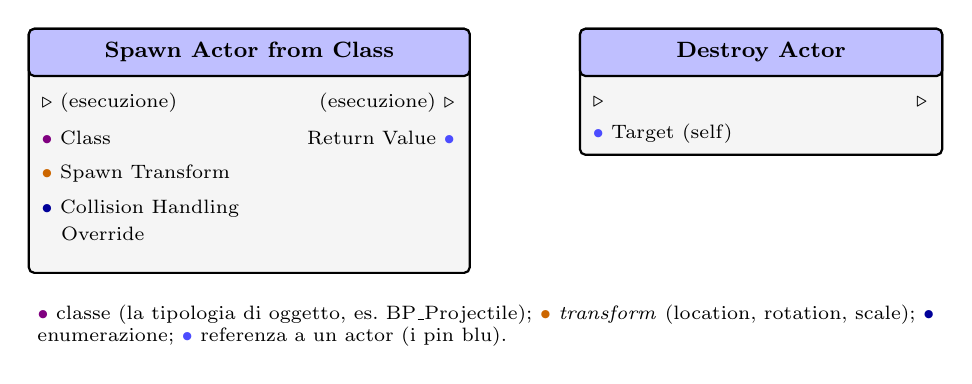
\begin{tikzpicture}[font=\footnotesize,
  ue5hdr/.style={draw, thick, fill=blue!25, minimum width=4.6cm, minimum height=0.6cm,
                 font=\footnotesize\bfseries, rounded corners=2pt},
  ue5bodyb/.style={draw, thick, fill=gray!8, minimum width=4.6cm, rounded corners=2pt},
  ue5pin/.style={font=\scriptsize, anchor=west},
  ue5pino/.style={font=\scriptsize, anchor=east}]
  % --- Spawn Actor from Class
  \node[ue5bodyb, minimum height=3.1cm, minimum width=5.6cm, anchor=north west] (sb)
    at (0,0) {};
  \node[ue5hdr, minimum width=5.6cm, anchor=north west] at (0,0) {Spawn Actor from
    Class};
  \node[ue5pin] at (0.05,-0.95) {$\triangleright$ (esecuzione)};
  \node[ue5pin] at (0.05,-1.4) {\textcolor{violet}{$\bullet$} Class};
  \node[ue5pin] at (0.05,-1.85) {\textcolor{orange!80!black}{$\bullet$} Spawn Transform};
  \node[ue5pin] at (0.05,-2.3) {\textcolor{blue!60!black}{$\bullet$} Collision Handling};
  \node[ue5pin] at (0.3,-2.62) {Override};
  \node[ue5pino] at (5.55,-0.95) {(esecuzione) $\triangleright$};
  \node[ue5pino] at (5.55,-1.4) {Return Value \textcolor{blue!70}{$\bullet$}};
  % --- Destroy Actor
  \node[ue5bodyb, minimum height=1.6cm, anchor=north west] at (7.0,0) {};
  \node[ue5hdr, anchor=north west] at (7.0,0) {Destroy Actor};
  \node[ue5pin] at (7.05,-0.95) {$\triangleright$};
  \node[ue5pin] at (7.05,-1.35) {\textcolor{blue!70}{$\bullet$} Target (self)};
  \node[ue5pino] at (11.55,-0.95) {$\triangleright$};
  % --- legenda
  \node[align=left, font=\scriptsize, anchor=north west, text width=11.4cm] at (0,-3.4)
    {\textcolor{violet}{$\bullet$} classe (la tipologia di oggetto, es.\ BP\_Projectile);
     \textcolor{orange!80!black}{$\bullet$} \emph{transform} (location, rotation,
     scale); \textcolor{blue!60!black}{$\bullet$} enumerazione;
     \textcolor{blue!70}{$\bullet$} referenza a un actor (i pin blu).};
\end{tikzpicture}
\caption{I due nodi della slide sullo spawn: in ingresso la classe da creare, il
\emph{transform} e il modo di gestire le collisioni; in uscita, la referenza all'actor
appena creato. Destroy Actor prende solo l'actor da distruggere. I colori dei pin
seguono le convenzioni dell'editor. Schema ricostruito.}
\label{ue5:fig:spawnnodes}
\end{figure}

\paragraph{Approfondimento: Collision Handling Override.} Il menù a tendina decide che
cosa fare se, nel punto di spawn, l'actor si troverebbe compenetrato con qualcos'altro.
Le opzioni sono: \emph{Default} (usa l'impostazione della classe), \emph{Always Spawn,
Ignore Collisions} (spawna comunque, anche dentro un muro), \emph{Try To Adjust
Location, But Always Spawn} (prova a spostarlo un poco, altrimenti spawna lì),
\emph{Try To Adjust Location, Don't Spawn If Still Colliding} (prova a spostarlo, e se
non trova posto non lo crea) e \emph{Do Not Spawn} (se c'è collisione, niente spawn).
Romero e Sewell (capitolo 3) suggeriscono anche di \textbf{promuovere a variabile} il
Return Value (tasto destro, \emph{Promote to Variable}) se l'oggetto creato servirà più
tardi, per esempio per distruggerlo; prima di usarla, la variabile va controllata con
un \textbf{Is Valid}, perché l'actor potrebbe essere già stato distrutto.

% ---------------------------------------------------------------------
\section{I cicli e il For Loop}
\label{ue5:sec:cicli}

``Anche un'altra cosa che andremo a vedere oggi sarà il \textbf{for loop}. Qualcuno ha
mai sentito parlare di \textbf{cicli} in programmazione?'' Uno studente che ha studiato
il C (``conosco \emph{while}, \emph{do while}, \emph{for}'') dà la definizione: ``è
ripetere un insieme di linee di codice finché una condizione è soddisfatta''. E fa un
esempio sulla torretta: ``finché il player sta in range della torretta, la torretta si
deve muovere; appena esce, quel codice non deve essere più ripetuto''. ``Sì,
assolutamente.''

Oggi, spiega il docente, si costruirà un actor che spawna dei cubetti ``in linea e in
colonne'': ``fondamentalmente andiamo a fare una \textbf{matrice}'', ``come in Excel,
ragazzi: le matrici per righe e colonne''. E lo si farà ``non uno per uno, ma tramite un
\textbf{indice}'': il For Loop è ``un modo iterativo di eseguire il codice fino a che
l'indice, quindi un numero che fa da dire OK, fatto il primo, OK, fatto il secondo, OK,
fatto il terzo\ldots{} Se arrivi a 10, smetti''. I cicli, infine, ``possono essere
innestati: cicli dentro altri cicli'', ed è esattamente ciò che servirà per righe e
colonne.

\paragraph{Approfondimento: i cicli dei Blueprint.} Nei Blueprint i cicli sono nodi di
\emph{flow control}. \textbf{For Loop} ha due ingressi interi, \textbf{First Index} e
\textbf{Last Index}, ed esegue il pin \textbf{Loop Body} una volta per ogni valore
dell'indice, dal primo all'ultimo \emph{compresi}, esponendo il valore corrente sul pin
\textbf{Index}; alla fine esegue \textbf{Completed}. \textbf{For Each Loop} fa lo stesso
scorrendo gli elementi di un array (Romero e Sewell, capitolo 13, lo usano per accendere
tutte le luci di una stanza). \textbf{While Loop} ripete finché una condizione booleana
è vera, come il \emph{while} del C. Una cosa importante, che distingue i cicli dei
Blueprint dal tempo del gioco: un For Loop si esegue \textbf{tutto nello stesso
\emph{frame}}, non ``piano piano nel tempo''. Non può contenere un Delay, e un ciclo
troppo lungo (o un While che non finisce mai) blocca il gioco; Unreal lo interrompe con
un errore di \emph{infinite loop} dopo un numero massimo di iterazioni. Per ripetere
qualcosa nel tempo si usano il Tick o i timer, come la torretta della quarta lezione.

% ---------------------------------------------------------------------
\section{Il fix della torretta: Find Relative Look at Rotation}
\label{ue5:sec:relative}

Prima dei proiettili, ``andremo a fissare una piccola cosa''. Il problema è quello visto
la volta scorsa: la torretta è fatta di tre \emph{static mesh}, e a ruotare è un solo
\emph{componente}, il Pivot, che ruota \textbf{rispetto al suo genitore}, la base. Find
Look at Rotation, invece, ``prenderà la rotazione in confronto a quella del
\textbf{mondo}, cioè di come è posizionato nel mondo''. Finché la torretta non è ruotata
nel livello le due cose coincidono; ma ``io giro la torretta a 90 gradi in engine, e poi
mi fa un offset di 90''.

\paragraph{La scoperta.} ``Ho scoperto, ed è una bellissima cosa, oserei dire, che Unreal
ci mette a disposizione il \textbf{Find Relative Look at Rotation} direttamente.'' Il
nodo ``prende il suo \emph{transform} e ci fa a quel punto un Find Look at Rotation in
relativa''. In pratica, in MoveTurret (il Custom Event chiamato dal timer):
\begin{itemize}
  \item si fa apparire \textbf{Find Relative Look at Rotation} al posto di Find Look at
        Rotation;
  \item al \textbf{Target} si collega quello che c'era già: la posizione del
        bersaglio, Get Actor Location di PlayerTarget;
  \item allo \textbf{Start Transform}, che chiede ``da che \emph{transform}
        partiamo'', si collega \textbf{Get Actor Transform} della torretta;
  \item l'uscita resta splittata, con la sola \textbf{Z} (lo \emph{yaw}) collegata al
        Target di \textbf{RInterp To}: ``questo non cambia assolutamente nulla''.
\end{itemize}
``Facendo ciò, da quel punto in poi la nostra torretta la possiamo ruotare come ci pare.
Tanto lui prenderà sempre a livello relativo.'' Il docente gira la torretta nel livello,
entra nel raggio: ``ecco che ci segue, senza cambiamenti, senza niente''
(figura~\ref{ue5:fig:relative}).

\paragraph{La velocità di interpolazione.} Il docente aveva trasformato l'Interp Speed in
una variabile e ``vi dico già che 0,01 era molto basso. Con questo find relative, ho
messo \textbf{2} e mi va più che bene. È anche più corretto''. A uno studente che non
sapeva come fosse nata la variabile: ``tira fuori dal pin, c'è scritto \emph{Promote to
Variable}''; poi si compila e, in basso a destra, nel \emph{Default Value}, si mette 2.
E, ``intanto'', il \textbf{Delta Time}: ``tira fuori dal Delta Time un pin e fai
\textbf{Get World Delta Seconds}''.

\begin{figure}[htbp]
\centering
\begin{tikzpicture}[font=\footnotesize,
  ue5node/.style={draw, thick, rounded corners=4pt, align=center, fill=gray!8,
                  minimum height=0.85cm, text width=2.4cm},
  ue5event/.style={ue5node, fill=red!12},
  ue5exec/.style={-{Stealth[length=2.5mm]}, very thick, black!80},
  ue5data/.style={-{Stealth[length=2mm]}, thick, blue!60!black},
  ue5trf/.style={-{Stealth[length=2mm]}, thick, orange!80!black},
  ue5flt/.style={-{Stealth[length=2mm]}, thick, green!50!black}]
  \node[ue5event] (mv) at (0,0) {\textbf{Custom Event}\\\textbf{MoveTurret}};
  \node[ue5node] (iv) at (3.1,0) {\textbf{Is Valid}\\PlayerTarget};
  \node[ue5node, text width=2.9cm] (srr) at (11.0,0) {\textbf{Set Relative
    Rotation}\\Target: Pivot};
  \draw[ue5exec] (mv) -- (iv);
  \draw[ue5exec] (iv) -- node[above, font=\scriptsize]{Is Valid} (srr);
  % dati
  \node[ue5node, fill=orange!12] (gat) at (0,-2.2) {\textbf{Get Actor
    Transform}\\(self)};
  \node[ue5node] (gal) at (0,-3.6) {\textbf{Get Actor Location}\\di PlayerTarget};
  \node[ue5node, text width=3.0cm, fill=yellow!20] (frl) at (3.6,-2.9)
    {\textbf{Find Relative Look at Rotation}\\Start Transform\\Target};
  \node[ue5node, text width=2.8cm] (ri) at (7.4,-2.9) {\textbf{RInterp To}\\
    Current: Get Relative Rotation (Pivot)\\Target: solo Z};
  \node[ue5node] (gwd) at (7.4,-5.0) {\textbf{Get World Delta Seconds}};
  \node[ue5node] (spd) at (4.1,-5.0) {\textbf{InterpSpeed}\\(variabile, 2)};
  \draw[ue5trf] (gat) -- (frl);
  \draw[ue5data] (gal) -- (frl);
  \draw[ue5flt] (frl) -- node[above, font=\scriptsize]{Z} (ri);
  \draw[ue5flt] (gwd) -- node[right, font=\scriptsize]{Delta Time} (ri);
  \draw[ue5flt] (spd) -- node[below, font=\scriptsize, pos=0.7]{Interp Speed} (ri);
  \draw[ue5flt] (ri.east) -| (srr.south);
\end{tikzpicture}
\caption{MoveTurret dopo il \emph{fix}. Il nodo nuovo (in giallo) calcola la rotazione
verso il bersaglio nello spazio della torretta, a partire dal suo \emph{transform}:
la torretta si può girare nel livello senza offset. Delta Time viene ora da Get World
Delta Seconds e l'Interp Speed, promosso a variabile, vale 2. Schema ricostruito.}
\label{ue5:fig:relative}
\end{figure}

\paragraph{Lo studente con la torretta che non gira.} Il primo caso in condivisione è
quello di uno studente che ha perso le lezioni precedenti per un problema al computer.
Il pivot non era stato reimportato a $-113$ (``non me l'ha fatto fare'', il re-import
non partiva). Lo si reimporta trascinando il file del materiale didattico nel
\emph{Content Browser} (attenzione a non lasciarlo cadere sopra altre cartelle); poi, in
scena, il pivot è ``storto'': lo si raddrizza con la modalità \textbf{Modeling}
(\textbf{Shift+5}), strumento \textbf{XForm}, \emph{Edit Pivot}. Nel Blueprint il pivot è
``un po' interrato'', e il cannone va staccato e riattaccato. Alla fine ruota, ``c'è un
piccolo offset, ma è importante che ruoti'', e punta ``dall'altra parte'': il caso è
rimandato alla pausa (sezione~\ref{ue5:sec:pausa}).

\paragraph{Approfondimento: perché il nodo nuovo risolve.} Find Relative Look at
Rotation (\emph{Start Transform}, \emph{Target Location}) trasforma prima il punto
bersaglio nello spazio locale del \emph{transform} di partenza, e poi calcola la
rotazione per guardarlo da lì. Il risultato è quindi già una rotazione
\textbf{relativa} all'actor, la stessa grandezza che Set Relative Rotation imposta sul
Pivot: i due spazi, che nel grafo della quarta lezione erano mescolati, ora coincidono.
Restano due avvertenze. Il punto di partenza è l'origine dell'actor, la base: va bene
per lo \emph{yaw}, ma per un \emph{pitch} preciso converrebbe partire dal
\emph{transform} del Pivot o del cannone (Get World Transform sul componente). E l'offset
dovuto alla \emph{mesh} reimportata a 113 gradi resta: il nodo presuppone che la
torretta, a rotazione zero, guardi lungo la propria X. Quanto alla velocità: con Delta
Time preso da Get World Delta Seconds e Interp Speed 2, il prodotto è circa 0,02 a 100
\emph{frame} al secondo, e la torretta insegue in modo morbido e uguale su ogni
macchina, come anticipato nella lezione precedente.

% ---------------------------------------------------------------------
\section{I trace: linee immaginarie}
\label{ue5:sec:trace}

``Abbiamo parlato di spawn, ma anche una cosa che andremo a vedere è chiamata
\textbf{line trace}.'' ``Oggi usiamo lo \textbf{sphere trace}, però in generale un trace
è una \textbf{linea immaginaria} che viene fatta dall'engine'' per scoprire che cosa c'è
lungo un percorso.

\paragraph{La dimostrazione.} Il docente lo mostra con la torretta che aveva già
preparato (``ecco qua, spawnano la marea di proiettili''). Entrando nel raggio, davanti
al cannone compare un \textbf{reticolo rosso}: ``una linea immaginaria, che non vedremo
se dovessimo avere un eseguibile''. Ma ``vedete che è rosso, rosso, rosso; se
\emph{overlappa}, diventa \textbf{verde}. Dice: ah, ho visto qualcosa! E quindi comincia
a sparare''. Poi, per confronto, trasforma al volo lo sphere trace in un \textbf{Line
Trace by Channel}: ``facciamo una linea''. All'inizio la linea non trova nulla, ``perché
è impostata male''; basta cambiarle il canale, e ``ecco che ci ha trovato'': ``fa rosso
il puntino e verde. Dice: ah, ok, ti ho beccato''.

\paragraph{A che cosa servono.} ``Sono delle linee immaginarie che servono a noi
\emph{developer} per dire: oh, c'è qualcosa che overlappa una linea invisibile?
Effettivamente sì, effettivamente no.'' Il docente racconta di averle usate per
un'intelligenza artificiale: ``tracciavo una linea tra me e il player; se c'era qualcosa
di mezzo, vuol dire che non lo vedeva; se invece non c'era niente, vuol dire che lo
vedeva''. È ``proprio una \textbf{linea di vista}''. E un avvertimento, ripetuto:
``non esagerate con il trace, perché anche esso è molto pesante'', tanto più se, come
oggi, lo si fa a ogni \emph{frame}.

\paragraph{Approfondimento: le famiglie di trace.} Romero e Sewell (capitolo 14)
definiscono i trace come test di collisione lungo un segmento. Ne esistono di due
tipi di ``filtro'': \textbf{by Channel}, che cercano gli oggetti che bloccano un
\emph{trace channel} (Visibility, Camera o un canale creato da noi), e \textbf{for
Objects}, che cercano gli oggetti di certi \emph{object type} (WorldStatic,
WorldDynamic, Pawn, PhysicsBody, Vehicle, Destructible). E di quattro forme: la
\textbf{linea}, la \textbf{sfera}, la \textbf{capsula} e il \textbf{box}, dove le forme
``spesse'' sono più costose della linea. Infine, ogni trace ha una versione singola,
che restituisce il primo oggetto colpito, e una \textbf{Multi}, che li restituisce
tutti (sezione~\ref{ue5:sec:errori}). Tutti hanno gli stessi ingressi principali:
\textbf{Start} ed \textbf{End}, il canale o i tipi, \textbf{Trace Complex} (testare
contro la \emph{mesh} vera o contro le forme di collisione semplificate), \textbf{Actors
to Ignore}, \textbf{Draw Debug Type} e \textbf{Ignore Self}. Le uscite sono un
\textbf{Out Hit} (una struttura \emph{Hit Result} con, tra l'altro, il punto d'impatto,
la normale della superficie e l'actor colpito, leggibili con \emph{Break Hit Result}) e
un \textbf{Return Value} booleano: vero se qualcosa ha bloccato il trace.

% ---------------------------------------------------------------------
\section{L'evento Shoot e i vettori del trace}
\label{ue5:sec:shoot}

``La prima cosa è che dobbiamo creare un evento \textbf{Shoot}'': un \textbf{Custom
Event} nel grafo di BP\_Turret.

\paragraph{Is Valid, per buona maniera.} ``Intanto la prima cosa che andiamo a fare è
vedere se esiste il target'': un \textbf{Is Valid} (``la macro con il punto
interrogativo'') su PlayerTarget. ``È buona maniera fare questa cosa, di vedere se
effettivamente esiste o non esiste, perché ci ottimizza i processi'': se non c'è un
bersaglio, non si esegue nulla. (Più avanti, nella sezione~\ref{ue5:sec:bocche}, questo
Is Valid verrà spostato fuori da Shoot.)

\paragraph{Lo Sphere Trace by Channel.} Poi lo \textbf{Sphere Trace by Channel}: ``una
linea immaginaria che andremo a creare in modo tale che, se il nostro character entra in
questa sfera, vuol dire che io lo sto vedendo ed è in puntamento''. Che cosa chiede?
``Un punto di \textbf{Start} e un punto di \textbf{End}'', con i pin
\textbf{gialli}. ``Chi si ricorda quali sono gli elementi gialli in Unreal?'' ``Un
vettore.'' ``Bravissimo, è un vettore. In questo caso, un vettore di locazione'': una X,
una Y e una Z.

\paragraph{Il punto di partenza: TraceSpawn.} Il trace deve partire ``più o meno dalla
canna, da questo punto qua in avanti''. Si potrebbe usare la posizione del Pivot, ``però
vi dico che è più corretto fare una cosa del genere: andiamo a creare proprio un
\textbf{punto vuoto}'' dedicato. Nei componenti si fa \emph{Add} e si scrive
\textbf{Scene}: un \emph{Scene Component}, ``solo un punto nello spazio'', senza
\emph{mesh} né collisioni. Lo si \textbf{attacca al cannone}, lo si posiziona ``in
mezzo alle due canne'', e lo si rinomina (``per rinominare le cose molto più
velocemente: cliccate sull'elemento, \textbf{F2}, e scrivete'') in
\textbf{TraceSpawn}. ``L'abbiamo attaccato al cannone perché il pivot fa ruotare il
cannone e il cannone farà ruotare il TraceSpawn: c'è questa \textbf{dipendenza a
cascata}.'' Dal componente TraceSpawn si prende \textbf{Get World Location}, ``dove è
posizionato nel mondo'', e la si collega allo \textbf{Start}.

\paragraph{Il punto d'arrivo: il forward vector.} ``Ci manca quello del punto di fine.
Dove deve arrivare?'' Qui torna la teoria dei vettori della quarta lezione. Ogni
\emph{mesh}, ogni componente, ogni actor ha dei vettori di direzione ``già prefatti'':
\begin{itemize}
  \item \textbf{Get Actor Forward Vector}, che ``punterà sempre in avanti'';
  \item \textbf{Get Actor Right Vector}, ``che punterà sempre a destra'';
  \item \textbf{Get Actor Up Vector}, ``che punterà sempre in alto'',
\end{itemize}
sempre relativi all'oggetto. ``Domanda: se io moltiplicassi per $-1$ il forward vector,
dove punterà rispetto alla mesh?'' ``Dietro.'' ``Bravissimo'': moltiplicare per $-1$
``inverte il risultato''; così si ottengono il \emph{back} vector, la sinistra e il
basso.

\paragraph{Lungo 1: moltiplicare.} Ma se si collega il forward vector così com'è ``non ci
darà assolutamente nulla, perché è molto piccolo'': ``il forward vector che ci dà Unreal
è di \textbf{lunghezza 1}'', un vettore normalizzato. ``Buona prassi è prenderlo e
moltiplicarlo, per esempio per \textbf{800}'': ``avremo un vettore 800 volte più
lungo''. (Uno studente non riesce a scrivere 800 nel Multiply: ``il pallino è giallo e
non verde''. ``Se moltiplicate un vettore, vi dà direttamente la moltiplicazione per un
altro vettore, ma potete cambiare il secondo fattore: tasto destro, \emph{To Float}.
Diventerà verde, e ci mettete 800.'')

\paragraph{Un punto non è una linea: sommare.} ``Magari vi verrebbe da dire: ok, ho
trovato il punto laggiù, lo vado a mettere nell'End. No, ancora no.'' Il forward vector
moltiplicato è ``un punto, non è una linea'': è uno spostamento di 800 in avanti,
calcolato come se si partisse dall'origine del mondo. ``Per farlo diventare una linea
dobbiamo letteralmente \textbf{sommare} due vettori'': la World Location di TraceSpawn
più il forward vector per 800. ``È un discorso che sembra strano, però effettivamente
quello che abbiamo qua è solo un punto nello spazio; con la somma ne traiamo un'effettiva
linea'' (figura~\ref{ue5:fig:vettori}).

\paragraph{Il forward vector giusto.} Alla prima prova il trace c'è, ma ``non segue il
pivot'': resta fermo mentre la torretta ruota. Il motivo: Get \emph{Actor} Forward
Vector è il vettore dell'actor intero, cioè della \textbf{base}, ``quindi sarà sempre lì.
Non girerà, perché deve girare insieme al cannone''. La correzione: ``invece di prendere
il Get Actor Forward Vector, prendiamo il \textbf{Get Forward Vector del TraceSpawn}''.
(``A me non fa collegare TraceSpawn e Get Forward Vector'': bisogna tirare il filo
\emph{dal} componente TraceSpawn e cercare \emph{Get Forward Vector}, la versione per i
componenti.)

\begin{figure}[htbp]
\centering
\begin{tikzpicture}[font=\footnotesize, >={Stealth[length=2.5mm]}]
  % assi del mondo
  \draw[->, thick, gray] (-0.3,0) -- (2.0,0) node[right]{X};
  \draw[->, thick, gray] (0,-0.3) -- (0,1.8) node[above]{Y};
  \node[below left, gray, font=\scriptsize] at (0,0) {origine del mondo};
  % torretta vista dall'alto
  \coordinate (C) at (6.0,0.4);
  \fill[gray!25, draw=black, thick] (C) circle (0.7);
  \node[font=\scriptsize, below] at ($(C)+(0,-0.7)$) {base};
  \begin{scope}[rotate around={35:(C)}]
    \fill[orange!25, draw=black, thick] ($(C)+(0,-0.2)$) rectangle ($(C)+(1.3,0.2)$);
  \end{scope}
  \coordinate (S) at ($(C)+(35:1.15)$);
  \fill[blue!60] (S) circle (0.07);
  \node[font=\scriptsize, align=center] at ($(S)+(-0.9,0.55)$) {TraceSpawn\\(Start)};
  % vettore posizione
  \draw[->, very thick, blue!60!black] (0,0) -- (S) node[pos=0.45, below, sloped,
    font=\scriptsize] {Get World Location};
  % forward unitario all'origine
  \draw[->, very thick, red!70!black] (0,0) -- (35:0.8);
  % forward x 800 all'origine (punto sbagliato)
  \draw[->, thick, red!70!black, dashed] (0,0) -- (35:3.6);
  \fill[red!70!black] (35:3.6) circle (0.06);
  \node[red!70!black, font=\scriptsize, align=left, anchor=south east] at (35:3.6)
    {Forward $\times$ 800\\(da solo: un punto\\vicino all'origine)};
  \node[red!70!black, font=\scriptsize, anchor=north west] at (0.15,-0.25)
    {Forward: lunghezza 1};
  % fine = start + forward x 800
  \coordinate (E) at ($(S)+(35:3.6)$);
  \draw[->, very thick, green!45!black] (S) -- (E);
  \fill[green!45!black] (E) circle (0.07);
  \node[right=3pt, green!45!black, align=left] at (E) {End =\\Start + Forward
    $\times$ 800};
  % sfera del trace
  \foreach \t in {0.2,0.45,0.7,0.95} {
    \draw[green!45!black, thin] ($(S)!\t!(E)$) circle (0.32);
  }
  \node[green!45!black, font=\scriptsize, anchor=west] at ($(S)!0.5!(E)+(0.45,-0.3)$)
    {Sphere Trace, Radius 80};
\end{tikzpicture}
\caption{I vettori del trace, visti dall'alto. Get World Location di TraceSpawn è un
vettore dall'origine del mondo al punto di partenza. Il Forward Vector è lungo 1;
moltiplicato per 800 diventa uno spostamento, che però, preso da solo, indica un punto
vicino all'origine (tratteggio). Sommato alla posizione di partenza, dà la fine giusta:
800 unità davanti alla canna. Lo sphere trace ``trascina'' una sfera di raggio 80 lungo
il segmento. Schema ricostruito, non in scala.}
\label{ue5:fig:vettori}
\end{figure}

\paragraph{Il raggio e il debug.} Due dettagli ancora. Il \textbf{Radius} dello sphere
trace parte da zero: ``il raggio della nostra bellissima sfera sarà zero, quindi non
esisterà''. Il docente mette \textbf{80}. E per vedere il trace in editor, ``lo vedremo
solo noi \emph{developer}'', c'è \textbf{Draw Debug Type}, da impostare su \textbf{For
One Frame}: ``perché se adesso la mettiamo \emph{For Duration}, ha una durata, sarà un
casino, perché lo fa ogni \emph{frame}'' (tabella~\ref{ue5:tab:debug}). Per provarlo,
Shoot viene chiamato dall'\textbf{Event Tick} (``prendete il Tick, scrivete Shoot,
come avete chiamato questo evento''): ``giusto per vedere effettivamente che
funzioni''.

\begin{table}[htbp]
\centering
\small
\begin{tabular}{@{}p{3.0cm}p{11.0cm}@{}}
\toprule
\textbf{Draw Debug Type} & \textbf{Che cosa disegna} \\
\midrule
None & niente: il trace c'è, ma non si vede (il valore di default) \\
For One Frame & il trace per un solo \emph{frame}: se il trace è chiamato a ogni
\emph{frame}, si vede ``in diretta''; è l'opzione usata a lezione \\
For Duration & il trace resta visibile per un certo tempo (Draw Time, nei dettagli del
nodo): chiamato a ogni \emph{frame}, accumula centinaia di disegni sovrapposti \\
Persistent & il trace resta disegnato per sempre: utile per un trace singolo, da
esaminare con calma \\
\bottomrule
\end{tabular}
\caption{Le opzioni di Draw Debug Type dei nodi di trace. I colori del disegno sono il
rosso per il tratto libero e il verde dal punto in cui il trace è stato bloccato (Trace
Color e Trace Hit Color, modificabili nel nodo).}
\label{ue5:tab:debug}
\end{table}

\paragraph{I problemi del momento.} Le condivisioni mostrano errori ricorrenti: lo
Start e l'End scambiati o collegati senza la somma (``Start è questo, solo questo; lo
attacchi così; il più va nell'End''); Draw Debug Type lasciato su \emph{None}; Shoot non
chiamato dal Tick (``l'hai messo sul Tick? Ah, no. Metti l'evento Shoot sul Tick''); e
la linea che compare ma non ruota con il cannone, per il motivo visto sopra.

% ---------------------------------------------------------------------
\section{I trace channel e le risposte di collisione}
\label{ue5:sec:canali}

Ora il trace c'è e ruota, ``ma come potete vedere non abbiamo il verdino, non ci dice
\emph{ho trovato}'': il player ci passa attraverso senza essere visto. Il motivo è il
\textbf{trace channel}. ``Di standard Unreal ci dà due canali, che sono
\textbf{Visibility} e \textbf{Camera}''; quello del docente (``questo qua al testo lo
vedete, l'ho creato io'') è un canale \textbf{custom}, che risponde ``in una certa
maniera, dipendentemente da certe opzioni''. Bisogna crearlo.

\paragraph{Creare il canale.} Dal menù \textbf{Edit}, \textbf{Project Settings}; si scende
``giù giù giù giù'' fino a \textbf{Collision} (nella sezione \emph{Engine}). Lì,
\textbf{New Trace Channel}: ``lo chiamate come volete, lo chiamiamo magari
\textbf{DetectionTurret}'', con \textbf{Default Response} su \textbf{Ignore}. Che cosa
vuol dire? ``Guarda questo trace: in risposta a tutti gli altri elementi in cui può
collidere, cosa fa di base? Ignora tutto, perché è meglio che ignori tutto, in modo tale
che tanto deve trovare solo il player.'' Se si mettesse \emph{Block}, ``ci bloccherebbe
tutto quanto'', e bisognerebbe togliere il blocco a tutti gli elementi statici e
dinamici. ``È più facile mettere ignora tutto, e poi mettiamo il \emph{tick} positivo al
nostro player.''

\paragraph{Il player risponde Block.} Si apre il \textbf{Third Person Character}, si
seleziona la \textbf{Mesh} e si cerca \emph{Collision} nei dettagli (``importante che, se
non avete compilato, compilate, perché se no non vi apparirà mai il nostro
DetectionTurret''). I \textbf{Collision Presets} sono grigi, perché è attivo un
\emph{preset}: si sceglie \textbf{Custom} dalla tendina, e nella riga di DetectionTurret
si mette la spunta su \textbf{Block}. ``In che modo reagisci al trace channel della
nostra torretta? Overlap, Block, Ignore. In questo caso andiamo a fare che blocca.''

\paragraph{Ignore, Overlap, Block.} Il docente ripassa le tre risposte con le mani:
``questa è la mia mano, l'oggetto 1, l'oggetto 2''. Con l'\textbf{Overlap}, ``se si
toccano non c'è una collisione fisica, quindi volendo si trapassano'', ma ``c'è una
\emph{detection}: l'engine dice, sono loro che collidono, quindi c'è un segnale''; è ciò
che si usa ``per i blocchi invisibili''. Il \textbf{Block}, invece, ``è proprio un
blocco fisico''. Il trace non ha un corpo, quindi per lui il Block è ``semplicemente
un'accortezza'': ``ehi, ho trovato il player, mi blocco''; ed è grazie al blocco che
appare la sfera ``parte verde, parte rossa'' (tabella~\ref{ue5:tab:risposte}).

\begin{table}[htbp]
\centering
\small
\begin{tabular}{@{}p{2.0cm}p{5.6cm}p{6.4cm}@{}}
\toprule
\textbf{Risposta} & \textbf{Tra due corpi} & \textbf{Per un trace} \\
\midrule
Ignore & si attraversano e nessuno se ne accorge & l'oggetto è invisibile per quel
trace \\
Overlap & si attraversano, ma scatta un evento di \emph{overlap} (i ``blocchi
invisibili'', la sfera della torretta) & il trace lo registra ma prosegue: lo vede solo
un trace Multi, e il Return Value resta falso \\
Block & si fermano l'uno contro l'altro: collisione fisica & il trace si ferma lì: è un
\emph{hit}, il disegno di debug diventa verde e il Return Value è vero \\
\bottomrule
\end{tabular}
\caption{Le tre risposte di collisione. Ogni componente dichiara una risposta per ogni
canale (Visibility, Camera, i canali custom) e per ogni \emph{object type}; quando due
oggetti si incontrano, vale la risposta più ``debole'' delle due.}
\label{ue5:tab:risposte}
\end{table}

\paragraph{Scegliere il canale nel trace.} Tornati in BP\_Turret, nello Sphere Trace by
Channel di Shoot si apre la tendina \textbf{Trace Channel}: ``c'è Visibility, Camera e
DetectionTurret''. Se compaiono solo Visibility e Camera, ``vai con \textbf{Compile},
qui in alto a sinistra''. In Play: ``vedete che è diventato verde. C'è il trace rosso,
viene bloccato, e da lì in poi c'è quello spazio verde'': ``è da lì in poi che il nostro
player è presente''. Avvicinandosi, il tratto verde si allunga.

\paragraph{Il Return Value.} Infine un \textbf{Print String} collegato al
\textbf{Return Value} del trace, ``che ci dice letteralmente: hai preso qualcosa? Sì,
no''. È un \textbf{booleano}: falso se non ha trovato niente, vero se ha trovato
qualcosa. In Play ``spunteranno un botto di true e false, ma è normale, sta sul Tick'':
``false, false, false\ldots{} true, true, true''.

\paragraph{Approfondimento: Mesh o Capsule?} A lezione la risposta Block al canale
DetectionTurret viene data alla \textbf{Mesh} del personaggio, e funziona. Nel Third
Person Character, però, il componente che rappresenta il corpo ai fini delle collisioni
è la \textbf{Capsule Component}, la radice; la Mesh scheletrica, di default, usa un
\emph{preset} (\emph{CharacterMesh}) pensato per non interferire con il movimento. Dare
il Block alla Mesh significa che il trace colpisce la forma del personaggio, con le sue
parti fisiche; darlo alla capsula significa colpire un cilindro più semplice. Entrambe
le scelte sono legittime; l'importante è sapere quale si è fatta, perché l'\emph{Hit
Actor} sarà lo stesso, ma l'\emph{Hit Component} e il punto d'impatto no.

% ---------------------------------------------------------------------
\section{Il proiettile: BP\_Projectile e il Projectile Movement}
\label{ue5:sec:proiettile}

``Abbiamo fatto la torretta che gira, abbiamo fatto la torretta che detecta: adesso
dobbiamo far sparare.'' Un Custom Event \textbf{SpawnProjectile}, ``ma che succede,
ragazzi? Non abbiamo un proiettile''. Lo si crea: tasto destro nel Content Browser,
\textbf{Blueprint Class}, \textbf{Actor}, e lo si chiama \textbf{BP\_Projectile}.

\paragraph{Due actor, due compiti.} Perché un Blueprint a parte, e non tutto dentro la
torretta? ``Due actor, uno che fa un compito e uno che fa un altro, è il miglior modo
per gestire i comportamenti.'' ``Perché a un certo punto magari vi arriva un
\emph{designer} e vi dice: ragazzi, non voglio che spawni più i proiettili, voglio che
spawni \textbf{banane}. Eh, se l'avete fatto dentro la torretta dovete fare un casino.
Invece, cambiare semplicemente il proiettile è molto più facile.''

\paragraph{La mesh.} Il proiettile è ``formato da due cose''. La prima è una \textbf{Static
Mesh}, rinominata \textbf{MeshProjectile}: una \textbf{sfera} di default (``se volete,
potete scaricare un modello, così ci mettete un proiettile al posto della palla'').
La si scala a \textbf{0,5}, poi a \textbf{0,3} (``mi sembra un po' grandicello''),
con il \textbf{lucchetto} della scala chiuso. ``Questo lucchetto l'abbiamo spiegato alla
prima lezione'': aperto, permette di modificare gli assi uno per uno; chiuso, ``se
modificate un singolo asse, vi scalerà anche le altre, in modo tale che rimangano
uniformi, perché sennò vengono forme stiracchiate''. Come materiale, \textbf{MI\_Solid\_Blue}
(``mi solid blue'').

\paragraph{Il Projectile Movement.} La seconda cosa è il movimento. ``Unreal ci arriva
con un regalo incredibile'': come la volta scorsa c'era il Rotating Movement per il
mulino, ``arriva la possibilità di avere un \textbf{Projectile Movement}, per quanti
giochi ormai hanno dei proiettili''. Si aggiunge il componente, e nei dettagli ci sono
``un sacco di dati in cui possiamo giocare'': ``tanti giochi ai giorni d'oggi hanno cose
molto comuni. Quanti FPS ce ne sono? Anche le armi di \emph{Borderlands}, che sono tutte
strane, alla base si parla sempre di sparare''. I valori della lezione:
\begin{itemize}
  \item \textbf{Initial Speed} 1000 e \textbf{Max Speed} 1000 (per guardarlo meglio, a
        un certo punto l'Initial Speed scende a 100, ``la lumaca'', e poi torna a 1000,
        ``una velocità da proiettile'');
  \item \textbf{Projectile Gravity Scale} a \textbf{0}: ``questo proiettile al momento
        è afflitto dalla gravità''; ``noi vogliamo che vada dritto per dritto'';
  \item \textbf{Velocity} lasciata a $(1, 0, 0)$: ``la velocità è la direzione'',
        quindi ``è 1 sull'asse X'', e il proiettile ``andrà dritto così''.
\end{itemize}
E la mesh deve essere \textbf{Movable}, ``se no vi danno errore''. Messo in scena e
avviato il Play, ``il nostro bellissimo proiettilino se ne va per la sua'' strada:
attraversa tutto, ``overlapperà, e chissà chi lo vedrà più''. (A una studentessa la
pallina ``cade semplicemente'': aveva lasciato la gravità a 1.)

\paragraph{Approfondimento: i parametri del Projectile Movement.} Romero e Sewell
(capitolo 6) modificano il proiettile del modello \emph{First Person} con gli stessi
parametri. \textbf{Initial Speed} è la velocità con cui il proiettile parte; \textbf{Max
Speed} è il limite, che conta solo se qualcos'altro lo accelera (un razzo con il motore
acceso); per un proiettile d'arma ha senso che le due coincidano. \textbf{Velocity} è
una direzione nello spazio \emph{locale} del proiettile: se Initial Speed è maggiore di
zero, Unreal ne usa solo la direzione e la moltiplica per l'Initial Speed. Per questo
è importante che lo spawn dia al proiettile la rotazione giusta: la X locale del
proiettile deve guardare fuori dalla canna. \textbf{Projectile Gravity Scale} moltiplica
la gravità del mondo (0 nessuna, 0,1 ``proiettile leggero''). La sezione \textbf{Projectile
Bounces}, con \emph{Should Bounce}, decide se rimbalza sui muri; e \textbf{Rotation Follows
Velocity} lo fa girare nella direzione del moto, utile per frecce e razzi.

% ---------------------------------------------------------------------
\section{Il proiettile che si distrugge}
\label{ue5:sec:distruzione}

``Noi vorremmo che il nostro proiettile sia molto più realistico: trova un muro e
scompare.'' E non è solo estetica: ``immaginatevi che adesso spawneremo dei proiettili
che andranno nell'infinito e oltre''; l'engine ``dirà: guarda, esiste'', e ``non
libereremo mai la memoria''.

\paragraph{Un trace attorno al proiettile.} La soluzione riusa il trace: nell'\textbf{Event
Tick} di BP\_Projectile, uno \textbf{Sphere Trace by Channel} di raggio \textbf{30},
``una sfera intorno al nostro proiettile che ci dirà: guarda, hai colpito qualcosa?''.
Start ed End sono \textbf{lo stesso punto}, \textbf{Get Actor Location} del proiettile:
``vogliamo che l'inizio e la fine siano lo stesso punto''. Con Draw Debug Type su For
One Frame, ``intorno alla nostra pallina si è creato un trace''.

\paragraph{Branch e Destroy Actor.} Poi: ``molto semplicemente, Return Value è vero? Sì?
Allora distruggete''. Un \textbf{Branch} (``tenete premuto B e cliccate'') sul Return
Value, e sul ramo True un \textbf{Destroy Actor} (figura~\ref{ue5:fig:proiettile}). In
Play, alla ``velocità della lumaca'', il proiettile arriva al muro e sparisce: ``si è
distrutto, quindi abbiamo il comportamento di base''. Il Tick, nota il docente,
``inizierà solamente quando l'oggetto esiste'': ogni proiettile controlla sé stesso
finché vive.

\begin{figure}[htbp]
\centering
\begin{tikzpicture}[font=\footnotesize,
  ue5node/.style={draw, thick, rounded corners=4pt, align=center, fill=gray!8,
                  minimum height=0.85cm, text width=2.5cm},
  ue5event/.style={ue5node, fill=red!12},
  ue5exec/.style={-{Stealth[length=2.5mm]}, very thick, black!80},
  ue5vec/.style={-{Stealth[length=2mm]}, thick, yellow!50!black},
  ue5bool/.style={-{Stealth[length=2mm]}, thick, red!60!black},
  ue5comp/.style={draw, thick, rounded corners=3pt, minimum width=3.5cm,
                  minimum height=0.55cm, align=center, font=\scriptsize}]
  % componenti
  \node[font=\scriptsize\bfseries] at (0,1.0) {BP\_Projectile: componenti};
  \node[ue5comp, fill=gray!20] (r) at (0,0.4) {DefaultSceneRoot};
  \node[ue5comp, fill=blue!20] (m) at (0.6,-0.3) {MeshProjectile (sfera, 0,3)};
  \node[ue5comp, fill=green!15] (pm) at (0,-1.0) {ProjectileMovement};
  \draw[thick, gray!60!black] ([xshift=-1.5cm]r.south) |- (m.west);
  \node[font=\scriptsize, align=left, anchor=west] at (-1.45,-1.75)
    {Initial / Max Speed 1000\\Gravity Scale 0, Velocity (1,0,0)};
  % grafo
  \node[ue5event] (tick) at (4.4,0.2) {\textbf{Event Tick}};
  \node[ue5node, text width=3.0cm] (st) at (7.9,0.2) {\textbf{Sphere Trace by
    Channel}\\Radius 30\\Channel: ProjectileTrace\\Debug: For One Frame};
  \node[ue5node, text width=1.6cm] (br) at (11.3,0.2) {\textbf{Branch}};
  \node[ue5node, text width=1.9cm] (de) at (11.3,-1.9) {\textbf{Destroy Actor}\\(self)};
  \node[ue5node] (gal) at (4.4,-1.6) {\textbf{Get Actor Location}\\(self)};
  \draw[ue5exec] (tick) -- (st);
  \draw[ue5exec] (st) -- (br);
  \draw[ue5exec] (br) -- node[right, font=\scriptsize]{True} (de);
  \draw[ue5vec] (gal.east) -| node[pos=0.75, left, font=\scriptsize, align=right]
    {Start\\e End} (st.south);
  \draw[ue5bool] ([yshift=-0.4cm]st.east) -- node[above, font=\scriptsize, pos=0.4]
    {Return Value} ([yshift=-0.4cm]br.west);
\end{tikzpicture}
\caption{Il proiettile. A sinistra i componenti: una sfera scalata e il Projectile
Movement, che fa tutto il moto. A destra il grafo: a ogni \emph{frame}, una sfera di
raggio 30 attorno al proiettile (Start ed End coincidono); se qualcosa la blocca, il
proiettile si distrugge. Il canale, all'inizio Visibility e poi Camera, diventa alla
fine ProjectileTrace. Schema ricostruito.}
\label{ue5:fig:proiettile}
\end{figure}

\paragraph{Approfondimento: altri modi di distruggere un proiettile.} Il trace sul Tick
funziona ed è istruttivo, ma non è l'unico modo, né il più economico. Il Projectile
Movement ha un proprio evento, \textbf{On Projectile Stop}, che scatta quando il
proiettile si ferma contro qualcosa che lo blocca; e un componente di collisione (una
Sphere Collision come radice del proiettile, con il Projectile Movement che la muove)
genera \textbf{Event Hit} o \textbf{On Component Hit} all'impatto. Romero e Sewell
(capitolo 6) collegano proprio all'evento di \emph{hit} il Destroy Actor, ``così che il
proiettile venga sempre distrutto quando collide''. Infine, per i proiettili che non
colpiscono nulla, l'actor ha una proprietà \textbf{Initial Life Span} (nei \emph{Class
Defaults}): se maggiore di zero, l'actor si distrugge da solo dopo quei secondi. È una
rete di sicurezza contro i proiettili che vanno ``nell'infinito e oltre''.

% ---------------------------------------------------------------------
\section{Visibility, Camera e il canale ProjectileTrace}
\label{ue5:sec:projtrace}

Il proiettile si distrugge contro il muro, ``anche il player, volendo?'' No: ``mi metto
davanti, e infatti non ce lo prende''. Con il canale \textbf{Visibility} il personaggio
non viene visto; cambiando il canale in \textbf{Camera}, ``così ci prende pure il
player''.

\paragraph{Perché.} Il docente apre le collisioni del Third Person Character: c'è la
tabella delle \textbf{Collision Responses}, con Ignore, Overlap e Block, e sotto le
\textbf{Trace Responses}, ``cioè come rispondo a questo trace''. ``Come rispondo al trace
Visibility? Vedete che c'è la spunta su Ignore; invece il Camera viene bloccato.''
``Semplicemente è un concetto di collisioni.''

\paragraph{Un canale per il proiettile.} ``Lo facciamo, ragazzi, così almeno è buona
prassi'': un secondo canale, \textbf{ProjectileTrace}. Qui il ragionamento è opposto a
quello di DetectionTurret. Il docente prima pensa a Ignore e a mettere il Block sui
quattro muri uno per uno (``però è più pesante''), poi cambia idea: ``è molto meglio
farlo in \textbf{Block}, così facciamo un Block e leviamo semplicemente quelli che non ci
interessano''. La regola generale: ``quante cose ho che devono bloccare, e quante che
devono ignorare?''. Il proiettile ``sbatte praticamente con tutto'', quindi Default
Response \textbf{Block}, e si escludono le poche eccezioni (tabella~\ref{ue5:tab:canali}):
\begin{itemize}
  \item il \emph{character}: Block (``va benissimo'');
  \item la \textbf{Sphere} della torretta, il raggio d'azione: Custom, ProjectileTrace
        su \textbf{Ignore}, altrimenti il proiettile esploderebbe appena nato, dentro la
        sfera;
  \item anche \textbf{Pivot}, \textbf{Base} e \textbf{Cannon}: ``non vogliamo che
        rimbalzi contro la stessa torretta che l'ha sparato'', quindi Custom e Ignore
        a tutti e tre.
\end{itemize}
Nel trace del proiettile si sceglie ProjectileTrace (``sempre compilato, perché se no non
vi arriva''), e in Play il proiettile si distrugge sia sul player sia sul muro.

\begin{table}[htbp]
\centering
\small
\begin{tabular}{@{}p{2.8cm}p{2.1cm}p{9.1cm}@{}}
\toprule
\textbf{Canale} & \textbf{Default} & \textbf{Eccezioni impostate a lezione} \\
\midrule
DetectionTurret & Ignore & Mesh del Third Person Character: \textbf{Block}. Il trace
della torretta vede solo il giocatore. \\
ProjectileTrace & Block & Sphere, Pivot, Base e Cannon della torretta: \textbf{Ignore};
dopo la pausa anche la sfera del proiettile stesso. Character: Block. Il proiettile si
ferma su tutto tranne che sulla torretta che lo spara. \\
\bottomrule
\end{tabular}
\caption{I due \emph{trace channel} creati in Project Settings $\rightarrow$ Engine
$\rightarrow$ Collision. Il principio: se le cose da colpire sono poche, Default
Ignore e Block sulle eccezioni; se sono molte, Default Block e Ignore sulle eccezioni.}
\label{ue5:tab:canali}
\end{table}

\paragraph{``A me passa attraverso.''} Due studenti hanno il proiettile che attraversa
player e muri (``il player me lo sposta, e i muri li attraversa''). Si controllano il
canale (Block), il nodo (ProjectileTrace), le collisioni della Mesh: tutto giusto. Il
colpevole è il \textbf{Radius}: ``era zero, quindi era invisibile''. ``Attenzione,
ragazzi, perché il radius è la grandezza: se è zero, non esiste.'' (E il raggio del
trace della torretta? ``80.'') Un'altra studentessa non trova i Collision Presets della
Sphere della torretta: bisogna selezionare proprio il componente \emph{Sphere} nella
lista dei componenti, e la sezione Collision compare.

\paragraph{Approfondimento: Ignore Self e Actors to Ignore.} Tutti i nodi di trace hanno
la casella \textbf{Ignore Self}, attiva di default: il trace ignora tutti i componenti
dell'actor che lo esegue. Il trace del proiettile, quindi, non vede la propria sfera
anche senza toccarne le collisioni, e quello della torretta non vede la torretta. Per
escludere \emph{altri} actor, senza modificare le loro collisioni, c'è l'ingresso
\textbf{Actors to Ignore}, un array: per esempio, il proiettile potrebbe ricevere allo
spawn una referenza alla torretta che l'ha sparato (i pin \emph{Owner} e \emph{Instigator}, che compaiono espandendo
Spawn Actor from Class, servono proprio a passare questo genere di informazione) e ignorarla nel trace. È la soluzione più pulita quando le torrette sono tante e
ognuna deve ignorare solo i propri colpi.

% ---------------------------------------------------------------------
\section{La pausa e i problemi degli studenti}
\label{ue5:sec:pausa}

Il docente crea il Custom Event SpawnProjectile e tira fuori \textbf{Spawn Actor from
Class}; poi guarda l'ora: ``sono le 17 e 28. Vogliamo fare pausa adesso, per fare lo
spawn dopo?'' La classe vota per la pausa, ``i classici 20 minuti'', alle 17:50. Ma chi
ha problemi resta, e la pausa diventa un lungo giro di condivisioni, utile soprattutto
per le tecniche di \emph{debug} che mostra.

\paragraph{Le collisioni della torretta.} Il primo caso è rapido: come si toglie la
collisione con il proiettile a Gun, Pivot e Base? ``Devi cliccare su ogni asset,
Collision Presets, fai Custom, Ignore a ProjectileTrace. A tutti e tre.''

\paragraph{Il Tick che non parte.} Il secondo caso è il più lungo, e resta irrisolto.
Uno studente non vede il trace della torretta in Play. Il docente prova, in ordine:
\begin{enumerate}
  \item un \textbf{breakpoint}: si seleziona il nodo Shoot e si preme \textbf{F9}, poi
        Play; se l'esecuzione arriva lì, l'editor si ferma e mostra il grafo (``quello è
        un \emph{breakpoint}; poi lo spiego in seguito''). Non si ferma: Shoot non viene
        mai eseguito;
  \item un \textbf{Print String} sul ramo \emph{Is Not Valid}, per capire se è il
        bersaglio a mancare; nel farlo, si scopre che sullo schermo compaiono già delle
        scritte, e le si insegue fino a un vecchio Print String dimenticato nel mulino;
  \item un Print String direttamente sull'\textbf{Event Tick}: dovrebbe ``spammare a
        manetta'', e invece niente. ``Si è rotto il Tick'';
  \item cancellare l'Event Tick e ricrearlo; chiudere e riaprire il Blueprint; cercare
        nei dettagli l'opzione di abilitazione del Tick (``scrivi \emph{enable}'');
        togliere l'actor dalla scena e rimetterlo;
  \item un Blueprint nuovo di prova, con solo Event Tick e Print String: quello
        funziona.
\end{enumerate}
``Diciamo che è un caso abbastanza particolare, ti posso dire la verità. Non riesco a
capire effettivamente perché il Tick non funzioni.'' La soluzione è pratica: il docente
comprime il proprio progetto e lo carica su \textbf{Classroom}, tra il materiale
didattico (``faccio tipo versione del 0406''), e lo studente riparte da quello.

\paragraph{Approfondimento: quando il Tick non parte.} Le cause più comuni, da
controllare in quest'ordine, sono: l'opzione \textbf{Start with Tick Enabled} (nei
\emph{Class Defaults}, sezione \emph{Actor Tick}) disattivata; un nodo \textbf{Set Actor
Tick Enabled} con il valore falso eseguito da qualche parte; un \textbf{Tick Interval}
diverso da zero, che fa scattare il Tick solo ogni tanto; un \emph{Event Tick} rimasto
\emph{scollegato} perché nel grafo ce n'è un altro (Unreal ne permette uno solo, e un
duplicato incollato compare come nodo disabilitato); e, nell'editor, l'istanza in scena
che non è il Blueprint modificato (una vecchia copia, o un Blueprint diverso con lo stesso
aspetto). Il test del Blueprint nuovo, fatto a lezione, è il modo giusto per separare un
problema del progetto da un problema dell'actor.

\paragraph{Il cannone che punta dall'altra parte.} Il terzo caso è lo studente della
sezione~\ref{ue5:sec:relative}: la torretta ruota, ma ``quando entra nella durezza''
(nel raggio) ``il cannone punta dall'altra parte del personaggio''. Nel grafo, Is Valid
e Find Relative Look at Rotation sono giusti. Il problema è la \emph{mesh} del pivot:
``è storto''. La reimportazione dà errore, quindi si usa il secondo metodo, la modalità
\textbf{Modeling} (\textbf{Shift+5}): nella colonna di sinistra, \textbf{XForm}, poi
\emph{Edit Pivot}, con \emph{Box Position} e la rotazione. ``Deve essere la \textbf{X}
dritta'': la freccia rossa del pivot deve puntare in avanti, lungo la canna. Attenzione
allo spazio del gizmo: ``metti il \textbf{Local} in alto a destra'' (invece di
\emph{World}). Dopo un paio di tentativi la torretta segue, ma ruotata di 180 gradi: si
corregge ruotando il cannone sull'asse \textbf{Z} (``la blu, usa la blu''). Resta il
trace che punta storto: TraceSpawn ha una rotazione di 42 gradi rimasta da qualche
spostamento; la si azzera (``la freccettina'' gialla accanto al valore, che riporta al
default), e ``è lui''.

\paragraph{Il trace che non gira e la sfera.} Il quarto caso: TraceSpawn non era figlio
del cannone (``probabilmente il TraceSpawn non è collegato al cannone, già lo vedo''): lo
si trascina sopra Cannon nella lista dei componenti. Poi la base non era la radice e la
Sphere non era figlia della base: si trascina la base sopra la radice e la sfera sopra la
base (``è la base, la dipendenza della sfera''). ``Se adesso nella viewport sposto la
torretta, si sposta anche la sfera?'' ``Sì.'' Per rendere la torretta più reattiva:
aumentare l'Interp Speed.

% ---------------------------------------------------------------------
\section{Lo spawn dei proiettili: le due bocche}
\label{ue5:sec:bocche}

Dopo il caffè, ``riprendiamo da dove abbiamo interrotto: dobbiamo spawnare i nostri
proiettili in una posizione in particolare''.

\paragraph{Due punti di spawn.} ``Il nostro cannone ha \textbf{due bocche}'', quindi due
\emph{Scene Component}: \textbf{ProjectileSpawn1} e, con Ctrl+C e Ctrl+V,
\textbf{ProjectileSpawn2} (``ne fa il numero in automatico''). Si attaccano al
\textbf{Cannon}, come TraceSpawn, e si posizionano ``all'uscita di ogni bocchetta''.

\paragraph{Spawn Actor from Class.} Nel Custom Event \textbf{SpawnProjectile}, il nodo
Spawn Actor from Class:
\begin{itemize}
  \item \textbf{Class}: dalla tendina, BP\_Projectile (``o come l'avete chiamato'');
  \item \textbf{Spawn Transform}: ``la nostra posizione, lì dove lo vogliamo far
        spawnare''. All'inizio il docente fa \emph{Split Struct Pin} (``ci dice Spawn
        Transform Location, Rotation e Scale'') e collega alla Location il \textbf{Get
        World Location} di ProjectileSpawn1; ``la rotazione non ci interessa, la scala
        non ci interessa. Anzi, no, facciamo per sicurezza'': ricombina il pin e usa
        \textbf{Get World Transform}, ``così ci diamo pure la rotation''.
\end{itemize}
La rotazione, in realtà, è essenziale: è lei a dire al proiettile dove sta ``davanti''
(la sua X locale, la direzione del Projectile Movement), quindi senza di essa i
proiettili partirebbero tutti lungo la X del mondo.

\paragraph{Collegare lo sparo: il trace decide.} ``Abbiamo la funzione, ma mettiamo:
hai trovato qualcosa?'' In Shoot, dopo lo Sphere Trace, un \textbf{Branch} sul Return
Value, e sul True la chiamata a \textbf{SpawnProjectile}. E l'Is Valid si sposta: ``prendete
questo Is Valid e spostiamolo da qui: Ctrl+X'', e lo si incolla \textbf{sull'Event
Tick}, prima della chiamata a Shoot. ``Perché è più ottimizzato? Perché la funzione di
per sé è a sé stante, ma il Tick parte a fare l'azione Shoot solamente se il player è
valido.'' In Play, i proiettili escono ``in un modo velocissimo'': uno a ogni
\emph{frame}.

\paragraph{Una bocca a caso: Select e Random Bool.} ``Dobbiamo farli spawnare da due
bocche, randomicamente.'' Si stacca ProjectileSpawn1, si tira fuori anche
ProjectileSpawn2, e si usa un \textbf{Select}: ``secondo un \emph{index}, che può essere
un intero, ma noi lo faremo booleano, selezionami l'actor da prendere''. Con l'indice
falso esce ProjectileSpawn1, con l'indice vero ProjectileSpawn2. All'indice si collega un
\textbf{Random Bool}: ``ogni volta che sparerà, tira fuori un booleano randomico tra vero
e falso''. Dall'uscita del Select si prende Get World Transform e lo si porta allo Spawn
Transform (figura~\ref{ue5:fig:sparo}).

\paragraph{Approfondimento: Select e i suoi parenti.} Il \textbf{Select} è un nodo
\emph{puro} (senza pin di esecuzione) che restituisce uno dei suoi ingressi in base a
un indice; le opzioni possono essere di qualsiasi tipo (qui referenze a componenti),
mentre l'indice può essere un intero, un booleano, un \emph{byte} o un'enumerazione
(Romero e Sewell, capitolo 15, lo usano per spawnare un boss diverso a seconda della
difficoltà). Le alternative: un \textbf{Flip Flop} alternerebbe le due bocche in modo
regolare, sinistra, destra, sinistra (Romero e Sewell lo mostrano proprio con due
pistole impugnate insieme, capitolo 13); un \textbf{Random Integer in Range} con un
Select a più opzioni servirebbe per un cannone a tre o quattro canne. Un dettaglio sui
nodi puri: vengono rivalutati ogni volta che un nodo li legge, quindi un Random Bool
collegato a due nodi diversi può dare due valori diversi nello stesso colpo; se il
risultato serve due volte, conviene salvarlo prima in una variabile.

% ---------------------------------------------------------------------
\section{Il fire rate: Do Once, Sequence e Delay}
\label{ue5:sec:firerate}

``E dargli un \textbf{fire rate}'': un proiettile al secondo, non uno per \emph{frame}.
La trascrizione di questo passaggio è frammentaria, ma i pezzi sono chiari, e così il
risultato mostrato in Play.

\paragraph{Il Delay.} Il primo strumento è un \textbf{Delay}: ``il delay sarà ogni quante
volte, cioè un secondo: ogni secondo mi spawno un proiettile''. Shoot è chiamato a ogni
\emph{frame}, ma un Delay già in corso ignora le nuove chiamate finché non è scaduto:
quindi passa al massimo uno sparo per intervallo. ``Però vi faccio vedere: se adesso io
vado davanti, aspetta un secondo e poi parte. Noi vogliamo che parta \textbf{subito},
appena mi vede.''

\paragraph{Do Once e Sequence.} Il secondo strumento è un \textbf{Do Once}, che lascia
passare l'esecuzione \emph{una sola volta} finché qualcuno non lo resetta; il terzo una
\textbf{Sequence}, che esegue in ordine le sue uscite. Il grafo che ne risulta, dopo il
Branch del trace:
\begin{itemize}
  \item \textbf{Then 0}: Do Once $\rightarrow$ SpawnProjectile, il colpo
        \emph{immediato}, appena la torretta vede il player;
  \item \textbf{Then 1}: Delay $\rightarrow$ SpawnProjectile, i colpi successivi,
        uno per intervallo.
\end{itemize}
Il Do Once va resettato quando il bersaglio sparisce, così il prossimo ingresso nel
raggio avrà di nuovo il colpo immediato: ``facciamo che si resetta il Do Once quando\ldots{}
Is Valid col player target, quando non è valido. Quindi: mi resetti''. Il ramo \textbf{Is
Not Valid} dell'Is Valid sull'Event Tick va al pin \textbf{Reset} del Do Once
(figura~\ref{ue5:fig:sparo}).

\paragraph{FireRate.} Infine la durata del Delay diventa una variabile: \emph{Promote to
Variable}, ``lo chiamo \textbf{FireRate}''. ``Vogliamo che sia più veloce? 0,5 secondi.''
``Pum, pum, pum, molto più veloce.'' ``Seguirà con lo sguardo, continuerà a spararci se
ci vede. Per adesso la torretta, con questo, è finita.'' Si potrebbero aggiungere ``un
sacco di cose, VFX, suoni, tutto quanto, però per quanto riguarda la programmazione è
completa''. (Più alto è il valore, più lungo è l'intervallo tra un proiettile e
l'altro: è una durata, non una frequenza.)

\begin{figure}[htbp]
\centering
\begin{tikzpicture}[font=\footnotesize,
  ue5node/.style={draw, thick, rounded corners=4pt, align=center, fill=gray!8,
                  minimum height=0.85cm, text width=2.2cm},
  ue5event/.style={ue5node, fill=red!12},
  ue5exec/.style={-{Stealth[length=2.5mm]}, very thick, black!80},
  ue5data/.style={-{Stealth[length=2mm]}, thick, blue!60!black},
  ue5bool/.style={-{Stealth[length=2mm]}, thick, red!60!black},
  ue5trf/.style={-{Stealth[length=2mm]}, thick, orange!80!black},
  ue5call/.style={-{Stealth[length=2mm]}, thick, dashed, gray!60!black}]
  % riga 1: tick
  \node[ue5event] (tick) at (0,0) {\textbf{Event Tick}};
  \node[ue5node] (iv) at (2.9,0) {\textbf{Is Valid}\\PlayerTarget};
  \node[ue5node] (shc) at (6.4,0) {\textbf{Shoot}\\(chiamata)};
  \draw[ue5exec] (tick) -- (iv);
  \draw[ue5exec] (iv) -- node[above, font=\scriptsize]{Is Valid} (shc);
  % riga 2: shoot
  \node[ue5event] (sh) at (0,-2.2) {\textbf{Custom Event}\\\textbf{Shoot}};
  \node[ue5node, text width=2.6cm] (st) at (3.0,-2.2) {\textbf{Sphere Trace by
    Channel}\\TraceSpawn, 800\\Radius 80\\DetectionTurret};
  \node[ue5node, text width=1.4cm] (br) at (5.6,-2.2) {\textbf{Branch}};
  \node[ue5node, text width=1.6cm] (seq) at (8.0,-2.2) {\textbf{Sequence}};
  \node[ue5node, text width=1.6cm] (do) at (10.5,-1.3) {\textbf{Do Once}};
  \node[ue5node, text width=1.9cm] (dl) at (10.5,-3.1) {\textbf{Delay}\\FireRate (0,5)};
  \node[ue5node, text width=2.4cm] (sp1) at (13.2,-1.3) {\textbf{SpawnProjectile}};
  \node[ue5node, text width=2.4cm] (sp2) at (13.2,-3.1) {\textbf{SpawnProjectile}};
  \draw[ue5exec] (sh) -- (st);
  \draw[ue5exec] (st) -- (br);
  \draw[ue5exec] (br) -- node[above, font=\scriptsize]{True} (seq);
  \draw[ue5exec] (seq.east) -- node[above, sloped, font=\scriptsize]{Then 0} (do.west);
  \draw[ue5exec] (seq.east) -- node[below, sloped, font=\scriptsize]{Then 1} (dl.west);
  \draw[ue5exec] (do) -- (sp1);
  \draw[ue5exec] (dl) -- (sp2);
  \draw[ue5bool] ([yshift=-0.35cm]st.east) -- ([yshift=-0.35cm]br.west);
  % reset
  \draw[ue5exec, red!60!black] (iv.north) -- ++(0,0.5) -| node[pos=0.25, above,
    font=\scriptsize]{Is Not Valid $\rightarrow$ Reset} (do.north);
  % riga 3: spawn projectile
  \node[ue5event, text width=2.6cm] (spe) at (0,-5.7) {\textbf{Custom Event}\\
    \textbf{SpawnProjectile}};
  \node[ue5node, text width=2.4cm] (ps1) at (3.1,-4.7) {ProjectileSpawn1};
  \node[ue5node, text width=2.4cm] (ps2) at (3.1,-5.7) {ProjectileSpawn2};
  \node[ue5node, text width=1.7cm] (rb) at (3.1,-6.7) {\textbf{Random Bool}};
  \node[ue5node, text width=1.9cm] (sel) at (6.0,-5.7) {\textbf{Select}\\False / True\\
    Index};
  \node[ue5node, text width=2.1cm] (gwt) at (8.6,-5.7) {\textbf{Get World
    Transform}};
  \node[ue5node, text width=2.9cm] (sa) at (12.1,-5.7) {\textbf{Spawn Actor from
    Class}\\Class: BP\_Projectile\\Spawn Transform};
  \draw[ue5exec] (spe.north) -- (0,-4.0) -| (sa.north);
  \draw[ue5data] (ps1.east) -- ([yshift=0.3cm]sel.west);
  \draw[ue5data] (ps2.east) -- (sel.west);
  \draw[ue5bool] (rb.east) -- ([yshift=-0.3cm]sel.west);
  \draw[ue5data] (sel) -- (gwt);
  \draw[ue5trf] (gwt) -- (sa);
\end{tikzpicture}
\caption{La torretta che spara. In alto: a ogni \emph{frame}, se c'è un bersaglio, si
chiama Shoot; se non c'è, si resetta il Do Once. In mezzo: Shoot lancia il trace; se
vede il player, spara subito una volta (Do Once) e poi una volta ogni FireRate secondi
(Delay). In basso: SpawnProjectile sceglie a caso una delle due bocche e vi crea un
proiettile, con la posizione e la rotazione della bocca. Schema ricostruito: l'ordine
esatto dei collegamenti tra Do Once, Sequence e Delay è dedotto dalla trascrizione e
dal comportamento mostrato in Play.}
\label{ue5:fig:sparo}
\end{figure}

\paragraph{Approfondimento: Delay, Do Once e i timer.} Romero e Sewell (capitolo 13)
descrivono il \textbf{Do Once} con l'esempio di un'arma caricata: alla pressione del
tasto spara una volta, e un timer chiama un evento che resetta il Do Once dopo trenta
secondi. È la stessa idea, a rovescio, del grafo della lezione. Il \textbf{Delay} è un
nodo \emph{latente}: sospende quel ramo di esecuzione e lo riprende dopo il tempo
indicato; chiamato di nuovo mentre conta, viene ignorato (a differenza del
\textbf{Retriggerable Delay}, che ricomincia a contare). I nodi latenti funzionano solo
nell'Event Graph, non nelle funzioni. L'alternativa più ``pulita'' a Delay e Do Once è
un \textbf{timer}, come quello che muove la torretta: all'ingresso del player si chiama
subito SpawnProjectile e si avvia un \textbf{Set Timer by Event} in \emph{loop} con Time
uguale a FireRate; all'uscita lo si ferma con \textbf{Clear and Invalidate Timer by
Handle}. Così niente lavora a ogni \emph{frame} se non serve.

% ---------------------------------------------------------------------
\section{Gli errori della ripresa e il Multi Sphere Trace}
\label{ue5:sec:errori}

``Adesso vediamo gli errori.''

\paragraph{Il proiettile che resta lì.} Prima della Sequence, due studenti avevano i
proiettili che restavano fermi davanti alla bocca, o sparivano appena usciti (``spara il
proiettile, però resta lì''; ``si distrugge appena esce''). Velocità: 1000, giusta.
Collisioni della torretta su Ignore: giuste. Uno dei due, con il Do Once e il Delay, se
lo vede risolto da solo: ``forse stava spawnando troppi proiettili assieme''. ``Bravissimo:
bisogna togliere la collisione a sé stesso''. Siccome ProjectileTrace blocca tutto, i
proiettili, uno per \emph{frame}, si colpivano tra loro: si va sulla sfera di
BP\_Projectile, Collision Presets \textbf{Custom}, ProjectileTrace su \textbf{Ignore},
``quindi fate ignorare anche loro stessi''. All'altra studentessa ``c'è la rete, come
se sparasse la rete del proiettile, però non c'è il proiettile'': si distrugge subito;
la causa è un componente della torretta senza Ignore su ProjectileTrace.

\paragraph{Approfondimento: perché i proiettili si distruggevano.} Ignore Self, come
visto, esclude dal trace i componenti dell'actor stesso, ma non \emph{gli altri}
proiettili. Con uno sparo per \emph{frame} e una sfera di trace di raggio 30, ogni
proiettile nasce praticamente dentro il precedente, e lo vede: si distruggono a vicenda.
Togliere a BP\_Projectile la risposta Block su ProjectileTrace li rende invisibili gli
uni agli altri, e risolve; rallentare il ritmo di fuoco, che allontana un proiettile
dall'altro, risolve anche da solo. Lo stesso accade se il raggio del trace del
proiettile (30) è più grande del proiettile stesso (una sfera di 100 unità scalata a 0,3
ha raggio 15) e la bocca è vicina a un componente che blocca: per questo il docente,
notando che ``i proiettili sono un po' più piccoli rispetto al trace'', suggerisce un
raggio ``di 10, di 20''.

\paragraph{Dove si cambia il fire rate.} ``Nella Sequence, il Delay: io l'ho fatto come
variabile, ma di base è la durata del Delay, la \emph{Duration}''. A chi manca la
variabile FireRate: dal pin Duration, \emph{Promote to Variable}, valore 0,5.

\paragraph{Sphere Trace e Multi Sphere Trace.} Uno studente si accorge di aver usato
\textbf{Multi Sphere Trace by Channel}. ``La differenza non ti cambia moltissimo, perché
è sempre uno sphere trace. Ma lo Sphere Trace si prende un oggetto; il Multi Sphere Trace
te ne prende di più: due, tre, quattro, cinque oggetti insieme'', ``una selezione a
gruppo invece di una selezione singola''. ``Se metti uno sphere trace e metti due player,
ti identificherà solo un player; se fai un multi sphere trace, ti riprende tutti e due.''
Quindi: lo Sphere Trace ``se dobbiamo prendere solamente un bersaglio, come il player'';
il Multi ``se dovessimo fare un check del tipo: ci devono essere almeno tre player per
far sì che la torretta spari''. Il riepilogo per chi si era perso: lo Start da
TraceSpawn, l'End con la somma, ``Radius a 80, Trace Channel DetectionTurret, Draw Debug
Type For One Frame''.

\paragraph{Approfondimento: che cosa restituisce un Multi.} Un trace Multi restituisce un
\textbf{array} di Hit Result, \textbf{Out Hits}, invece di uno solo. Con un canale, il
trace attraversa gli oggetti che rispondono \emph{Overlap} e li aggiunge alla lista, e si
ferma al primo che risponde \emph{Block}, che è l'ultimo elemento. Il Return Value è vero
solo se c'è stato un Block. Quindi, sul canale DetectionTurret dove il player
\emph{blocca}, due player in fila danno comunque un solo \emph{hit}, il primo: per
contarli tutti, il player dovrebbe rispondere Overlap e si dovrebbe leggere la lunghezza
dell'array (\emph{Length}). Romero e Sewell notano che le versioni Multi sono più costose
di quelle singole: si usano solo se servono davvero più risultati.

% ---------------------------------------------------------------------
\section{La torretta si ferma: On Component End Overlap}
\label{ue5:sec:endoverlap}

Uno studente fa notare che la torretta lo segue ``anche quando esco fuori'' dal raggio.
``È voluto, poi lo interrompiamo'': è il pezzo che manca dalla lezione precedente.
``Dobbiamo far sì che, quando il nostro player esce, la variabile del player target si
\textbf{svuoti}, in modo tale che non abbiamo più un target. La torretta quindi smette di
funzionare totalmente e si ferma.''

\paragraph{Il contrario del Begin Overlap.} Si seleziona la \textbf{Sphere}, si scende
nei dettagli fino agli eventi e si aggiunge (con il ``+'') \textbf{On Component End
Overlap}. È il gemello dell'evento della volta scorsa, che controllava che l'actor
entrato fosse valido e avesse il tag, e lo salvava come bersaglio. ``Adesso andremo a
fare letteralmente il contrario'': da \textbf{Other Actor}, \textbf{Actor Has Tag}
\emph{Player} (``l'abbiamo già messo''), un \textbf{Branch}, e sul True un \textbf{Set}
di \textbf{PlayerTarget} con il pin di ingresso \textbf{vuoto}: ``che vuol dire vuota?
Vuol dire che non è più valida. Così si setta una variabile vuota: semplicemente non
impostando niente'' (figura~\ref{ue5:fig:endoverlap}).

\paragraph{L'effetto a cascata.} Svuotata la variabile, tutti gli Is Valid del grafo
rispondono \emph{Is Not Valid}: MoveTurret non ruota più il Pivot, l'Event Tick non
chiama più Shoot, ``e quindi il Do Once si resetta, con il problema di prima''. In Play:
``noi usciamo, il trace scompare. E ricompare'', quando si rientra. ``Ed ecco che abbiamo
finito effettivamente la nostra torretta.''

\begin{figure}[htbp]
\centering
\begin{tikzpicture}[font=\footnotesize,
  ue5node/.style={draw, thick, rounded corners=4pt, align=center, fill=gray!8,
                  minimum height=0.85cm, text width=2.4cm},
  ue5event/.style={ue5node, fill=red!12},
  ue5exec/.style={-{Stealth[length=2.5mm]}, very thick, black!80},
  ue5data/.style={-{Stealth[length=2mm]}, thick, blue!60!black},
  ue5bool/.style={-{Stealth[length=2mm]}, thick, red!60!black}]
  \node[ue5event, text width=2.8cm] (eo) at (0,0) {\textbf{On Component End
    Overlap}\\(Sphere)};
  \node[ue5node, text width=1.5cm] (br) at (3.5,0) {\textbf{Branch}};
  \node[ue5node, text width=2.6cm] (set) at (6.6,0) {\textbf{Set PlayerTarget}\\
    (ingresso vuoto)};
  \node[ue5node] (tag) at (2.0,-1.8) {\textbf{Actor Has Tag}\\Tag: Player};
  \draw[ue5exec] (eo) -- (br);
  \draw[ue5exec] (br) -- node[above, font=\scriptsize]{True} (set);
  \draw[ue5data] (eo.south) |- node[pos=0.25, left, font=\scriptsize]{Other Actor}
    (tag.west);
  \draw[ue5bool] (tag.east) -| (br.south);
  \node[draw, dashed, rounded corners=4pt, align=left, text width=4.6cm,
        font=\scriptsize, fill=yellow!8] at (10.9,-0.6)
    {Da qui in poi PlayerTarget non è valido:\\
     $\bullet$ MoveTurret non ruota il Pivot;\\
     $\bullet$ l'Event Tick non chiama Shoot;\\
     $\bullet$ il Do Once viene resettato;\\
     $\bullet$ il timer di TrackTargetTimer, però,\\
     \phantom{$\bullet$ }continua a girare (vedi testo).};
\end{tikzpicture}
\caption{L'uscita dal raggio: se chi esce dalla sfera è il player, si svuota
PlayerTarget. Tutti i controlli Is Valid del resto del grafo fanno il resto. Schema
ricostruito.}
\label{ue5:fig:endoverlap}
\end{figure}

\paragraph{Approfondimento: svuotare una variabile, e il timer.} In un nodo \emph{Set}
di una referenza, lasciare il pin scollegato equivale ad assegnare \textbf{None}, il
valore ``nessun oggetto'': Is Valid, su None, dà Is Not Valid. Il timer avviato da
TrackTargetTimer nella quarta lezione, però, non viene fermato: continua a chiamare
MoveTurret a ogni \emph{frame}, e MoveTurret si limita a uscire subito dall'Is Valid. È
innocuo, ma è lavoro inutile, e al rientro del player il Begin Overlap ne avvia un altro
(Set Timer by Event con lo stesso evento sostituisce il timer precedente, quindi non si
accumulano). Il modo completo è salvare il \textbf{Return Value} di Set Timer by Event in
una variabile \emph{Timer Handle} e, nell'End Overlap, chiamare \textbf{Clear and
Invalidate Timer by Handle} oltre a svuotare PlayerTarget.

\paragraph{Che ne sarà della torretta.} ``Sappiate che la torretta la riuserete, perché
più in là farete delle lezioni con \textbf{Davide}'', sui \textbf{livelli}, e ``avrete
l'opportunità di usarla per fare un livellino'': ``un possibile opponente, un possibile
ostacolo''.

% ---------------------------------------------------------------------
\section{L'esercizio della matrice di cubi: il For Loop}
\label{ue5:sec:matrice}

``Abbiamo 20 minuti. Dobbiamo fare anche un altro esercizio: lo iniziamo oggi, lo
finiamo la prossima volta.'' Il docente mostra il risultato finale, già pronto: una
\textbf{matrice di cubi}, ``perfettamente allineati e spaziati tra di loro'', generata
da un actor vuoto ``usando la matematica e un ciclo \emph{for}''.

\paragraph{L'actor e l'evento.} Un nuovo Blueprint Class di tipo Actor (il nome, nella
trascrizione, è ``pp spawn più x'', qualcosa come \emph{BP\_SpawnX}), con subito un
Custom Event \textbf{SpawnerRow} e, collegato, un \textbf{For Loop} (``non For Each: For
Loop''), dalla categoria \emph{Flow Control}. \textbf{First Index} 1, \textbf{Last Index}
10, ``poi magari li cambieremo''.

\paragraph{Dall'indice alla posizione.} ``Andiamo a prendere l'\textbf{Index} e lo
moltiplichiamo per un tot'': per 100. A ogni giro l'indice cresce, ``1 per 100 diventa
100, 2 per 100 diventa 200, eccetera''. Questo numero si somma alla posizione
dell'actor: \textbf{Get Actor Location}, splittata, e la sua \textbf{X} più l'indice per
100. Il docente lo fa vedere a mano nei dettagli dell'actor: ``io adesso sto a 1975;
ci aggiungo 100, quindi sarà 2075: vedete che si muove di 100''; con l'indice 2, ``1975
più 200 sarà 2175''. ``Moltiplicando questo valore andremo a creare varie somme che sono
sequenziali.'' Con un \textbf{Make Vector} si ricompone il punto: la X nuova, la Y e la Z
dell'actor, invariate (figura~\ref{ue5:fig:matrice}).

\paragraph{Vedere i punti: un Line Trace.} Per ora non si spawna niente: si
\emph{visualizzano} le posizioni con un \textbf{Line Trace by Channel} (``questa sarà una
linea; prima era una sfera''), il cui \textbf{Start} è il Make Vector. Per l'\textbf{End}
serve un vettore che vada \emph{giù}: il docente prova prima a togliere 200 alla Z, poi
usa la rotazione dell'actor. \textbf{Get Actor Rotation}, da cui \textbf{Get Up Vector}
(``il vettore che va su''), moltiplicato per $-5000$: ``lo inverti moltiplicandolo per
meno 5000; non per meno 1, perché meno 1 è solo più piccolo''. Lo si somma al Make Vector
e lo si mette nell'End. Draw Debug Type For One Frame, e SpawnerRow chiamato dall'Event
Tick. In Play: ``guardate che abbiamo creato dei line trace perfettamente spaziati di 100
con un ciclo for''. ``Abbiamo già le posizioni dove potremmo spawnare eventualmente i
nostri cubetti.''

\begin{figure}[htbp]
\centering
\begin{tikzpicture}[font=\footnotesize,
  ue5node/.style={draw, thick, rounded corners=4pt, align=center, fill=gray!8,
                  minimum height=0.85cm, text width=2.2cm},
  ue5event/.style={ue5node, fill=red!12},
  ue5exec/.style={-{Stealth[length=2.5mm]}, very thick, black!80},
  ue5int/.style={-{Stealth[length=2mm]}, thick, cyan!60!black},
  ue5vec/.style={-{Stealth[length=2mm]}, thick, yellow!50!black}]
  % grafo
  \node[ue5event] (ev) at (0,0) {\textbf{Custom Event}\\\textbf{SpawnerRow}};
  \node[ue5node] (fl) at (2.9,0) {\textbf{For Loop}\\First 1, Last 10};
  \node[ue5node, text width=2.6cm] (lt) at (12.0,0) {\textbf{Line Trace by
    Channel}\\Debug: For One Frame};
  \draw[ue5exec] (ev) -- (fl);
  \draw[ue5exec] (fl) -- node[above, font=\scriptsize]{Loop Body} (lt);
  \node[ue5node, text width=1.7cm] (mul) at (2.9,-1.9) {Index $\times$ 100};
  \node[ue5node, text width=1.3cm] (add) at (5.4,-1.9) {+ X};
  \node[ue5node, text width=1.9cm] (mv) at (7.9,-1.9) {\textbf{Make Vector}\\X, Y, Z};
  \node[ue5node, text width=0.8cm] (sum) at (10.3,-1.9) {+};
  \node[ue5node, text width=2.2cm] (gal) at (5.4,-3.8) {\textbf{Get Actor
    Location}\\(split X, Y, Z)};
  \node[ue5node, text width=3.0cm] (up) at (10.3,-3.8) {\textbf{Get Actor Rotation}
    $\rightarrow$ \textbf{Get Up Vector} $\times(-5000)$};
  \draw[ue5int] (fl.south) -- node[right, font=\scriptsize]{Index} (mul.north);
  \draw[ue5int] (mul) -- (add);
  \draw[ue5int] (gal.north) -- node[right, font=\scriptsize]{X} (add.south);
  \draw[ue5int] (gal.east) -| node[pos=0.75, right, font=\scriptsize]{Y, Z} (mv.south);
  \draw[ue5int] (add) -- (mv);
  \draw[ue5vec] (mv) -- (sum);
  \draw[ue5vec] (mv.north) |- node[pos=0.75, below, font=\scriptsize]{Start}
    ([yshift=-0.25cm]lt.west);
  \draw[ue5vec] (up.north) -- (sum.south);
  \draw[ue5vec] (sum.east) -| node[pos=0.75, right, font=\scriptsize]{End} (lt.south);
  % vista laterale
  \begin{scope}[yshift=-6.4cm]
    \draw[thick, gray] (-0.3,-1.3) -- (11.8,-1.3);
    \node[font=\scriptsize, gray] at (11.3,-1.55) {pavimento};
    \fill[red!60] (0,0) circle (0.1);
    \node[font=\scriptsize, left] at (-0.15,0) {actor (X = 1975)};
    \foreach \i in {1,...,10} {
      \pgfmathsetmacro{\x}{\i*1.05}
      \draw[->, thick, red!70!black] (\x,0) -- (\x,-1.3);
      \fill[green!45!black] (\x,-1.3) circle (0.06);
    }
    \node[font=\scriptsize] at (1.05,0.35) {2075};
    \node[font=\scriptsize] at (2.1,0.35) {2175};
    \node[font=\scriptsize] at (10.5,0.35) {2975};
    \node[font=\scriptsize] at (6.3,0.35) {\ldots};
  \end{scope}
\end{tikzpicture}
\caption{L'esercizio della matrice, prima parte: una riga. Il For Loop conta da 1 a 10;
ogni indice, moltiplicato per 100 e sommato alla X dell'actor, dà un punto; da quel punto
parte un line trace verso il basso (l'Up Vector dell'actor invertito e allungato). Sotto,
il risultato visto di lato, con le X della lezione: dieci linee distanziate di 100 unità.
La prossima volta, al posto dei trace, i cubi, e un secondo ciclo per le colonne. Schema
ricostruito.}
\label{ue5:fig:matrice}
\end{figure}

\paragraph{I problemi.} ``A me le linee sono oblique'': bisogna usare la rotazione
dell'actor e il suo Up Vector, non un vettore qualunque. ``A me vanno verso l'alto'':
la studentessa aveva ruotato l'actor; ``non lo devi ruotare''. ``A me non si vedono
proprio'': l'actor era troppo vicino al pavimento, ``spostalo un po' più in alto'' e
guarda la scena dall'alto; ``l'importante è che vedi che i puntini sono spaziati tra di
loro''.

\paragraph{Perché proprio dieci.} ``Una cosa che non ho capito: perché ne spawnano
specificamente 10?'' ``Perché abbiamo l'indice a 10.'' Il For Loop parte dal
\textbf{First Index}, 1, e ``ogni volta che fa questa esecuzione, questo index aumenta di
1: farà 1, 2, 3''. ``Quando arriva al \textbf{Last Index}, 10, si ferma.'' Il docente
mette Last Index a 20 e conta le linee: ``sono più di 10, e sono 20''. ``Lo farà 20 volte,
fondamentalmente.'' La prossima volta: ``le righe, e per ogni riga andremo a spawnare di
nuovo altri elementi'', cioè un ciclo dentro l'altro.

\paragraph{Approfondimento: la matrice completa.} Romero e Sewell (capitolo 19) costruiscono
esattamente questa griglia nel \emph{Construction Script}, con due For Loop
\textbf{annidati}: il ciclo esterno conta le righe e calcola la X (indice $\times$
spaziatura tra le righe); il ciclo interno, eseguito per intero a ogni giro
dell'esterno, conta gli elementi della riga e calcola la Y (indice $\times$ spaziatura
tra gli elementi). Con $r$ righe e $c$ colonne il corpo interno si esegue $r \times c$
volte, e la posizione dell'elemento $(i, j)$ è
\[
  P_{ij} = P_0 + (i \cdot d_x,\; j \cdot d_y,\; 0),
\]
dove $P_0$ è la posizione dell'actor e $d_x$, $d_y$ le spaziature. Due differenze
rispetto alla lezione. La prima: il libro non spawna un actor per cubo, ma aggiunge
\emph{istanze} a un \textbf{Instanced Static Mesh Component} (nodo \emph{Add Instance}),
che disegna centinaia di copie della stessa \emph{mesh} con un costo minimo: è un
parente del \emph{pooling} visto a inizio lezione. La seconda: nel Construction Script
la griglia si aggiorna già nell'editor, cambiando righe e colonne nei dettagli; chiamare
la generazione dall'Event Tick, come per i trace di prova, va bene solo per il debug,
perché spawnare cubi a ogni \emph{frame} ne creerebbe migliaia.

% ---------------------------------------------------------------------
\section{La torretta che mira ai piedi, e la chiusura}
\label{ue5:sec:chiusura}

``Mancano 5 minuti.'' Una curiosità di uno studente, che aveva fatto muovere la canna
anche in alto e in basso: ``quando mi allontano, mira i piedi; quando mi avvicino, il
torso''. Come si mira più in alto?

\paragraph{Due soluzioni.} Il docente comincia a mostrarne una: invece di mirare
all'actor del player, aggiungere al Third Person Character un \emph{Scene Component}
vuoto, ``attaccato alla mesh'', sulla testa o sul collo, e mirare a quello (``mi sa che
ti tocca fare una referenza'' del tipo giusto, per poterne leggere i componenti). Ma uno
studente propone una soluzione più semplice, che aveva già trovato per lo stesso
problema: ``Find Relative Look at Rotation utilizza il pivot della \textbf{base}, non della
GAN''. Quindi ha misurato la differenza d'altezza tra il pivot della canna e quello della
base, e ha ``detto: prendi la location dell'actor e \textbf{abbassala}, nel mio caso di
100''. ``Ottima trovata. Bravo.'' Con una precisazione sugli assi: ``per la rotation è la
\textbf{Y}'' (il \emph{pitch}), ``ma per la location è la \textbf{Z}'' (l'altezza).

\paragraph{Approfondimento: perché la mira cambia con la distanza.} L'angolo di
\emph{pitch} calcolato da Find (Relative) Look at Rotation è quello della retta che va
dal punto di partenza al bersaglio. Se il punto di partenza è la base, più in basso della
canna di un'altezza $h$, e il bersaglio è a distanza orizzontale $d$, la canna viene
inclinata dell'angolo giusto per la base, non per sé stessa: l'errore è circa
$\arctan(h/d)$, grande quando il player è vicino e piccolo quando è lontano. Per questo
la mira ``scivola'' con la distanza. Le correzioni sono equivalenti nella sostanza: far
partire il calcolo dalla posizione della canna (il \emph{transform} del Pivot o di
TraceSpawn), oppure spostare il punto di partenza o il bersaglio della stessa differenza
d'altezza, come ha fatto lo studente. Mirare a un punto del corpo (la testa, il busto)
invece che all'origine dell'actor risolve il problema opposto: l'origine del Third Person
Character è al centro della capsula, a metà altezza.

\paragraph{La chiusura.} ``Ottimo, perfetto, ragazzi. Ci sentiamo la prossima volta.
Qualsiasi domanda in mente, potete farla tranquillamente sul \textbf{Discord}.'' Uno
studente chiede di ripartire, la volta dopo, dalla matrice: ``mi funziona tutto, ma non ho
capito il ragionamento logico dietro certi nodi''. ``Tanto la prossima volta sicuramente
partiremo un attimo dall'inizio, perché abbiamo fatto lo spawn, poi dobbiamo fare subito
un altro argomento, e diciamo che a fine lezione la mente fresca viene meglio.''
L'appuntamento è per \textbf{martedì}. ``Dai, ragazzi, buona serata.''

\begin{table}[htbp]
\centering
\small
\begin{tabular}{@{}p{5.4cm}p{8.6cm}@{}}
\toprule
\textbf{Sintomo} & \textbf{Causa e rimedio} \\
\midrule
Materiali neri dopo la riapertura & la texture del materiale manca: riassegnarla (e
salvare tutto dall'indicatore in basso a destra) \\
La torretta guarda di lato se ruotata nel livello & Find Look at Rotation lavora nel
mondo: usare Find Relative Look at Rotation con Get Actor Transform \\
La torretta punta dall'altra parte & la \emph{mesh} del pivot non guarda lungo X:
reimportarla o correggerne il pivot (Modeling, XForm, Edit Pivot, gizmo in Local) \\
Il trace non si vede & Draw Debug Type su None; Radius a 0; Shoot non chiamato
dall'Event Tick \\
Il trace non ruota con il cannone & Get Actor Forward Vector (della base) invece del
Forward Vector di TraceSpawn; TraceSpawn non figlio del Cannon; rotazione residua su
TraceSpawn \\
Il trace non diventa verde sul player & il player non risponde Block al canale: Collision
Presets Custom, DetectionTurret su Block; compilare prima \\
Il canale custom non compare nel nodo & compilare il Blueprint \\
Il Multiply non accetta 800 & il secondo pin è un vettore: tasto destro, convertirlo
in \emph{float} \\
Il proiettile cade & Projectile Gravity Scale ancora a 1 \\
Il proiettile attraversa tutto & Radius del suo trace a 0; canale sbagliato (Visibility
non vede il player) \\
Il proiettile sparisce appena nato & un componente della torretta (Sphere, Pivot, Base,
Cannon) o il proiettile stesso non ignora ProjectileTrace \\
Spawn di un proiettile per \emph{frame} & manca il \emph{fire rate}: Delay (e Do Once
per il primo colpo) \\
Il primo colpo arriva in ritardo & solo il Delay: aggiungere Do Once con Reset sull'Is
Not Valid \\
La torretta continua dopo l'uscita & manca On Component End Overlap che svuota
PlayerTarget \\
L'Event Tick non scatta & caso irrisolto a lezione: controllare Start with Tick Enabled,
Set Actor Tick Enabled, Tick Interval, l'istanza in scena \\
Le linee della matrice sono oblique o vanno su & usare Get Up Vector della rotazione
dell'actor, moltiplicato per un valore negativo; non ruotare l'actor \\
La canna mira ai piedi da lontano & il calcolo parte dalla base: abbassare la location di
partenza (o partire dalla canna) \\
\bottomrule
\end{tabular}
\caption{I problemi incontrati durante la lezione, con la causa e il rimedio.}
\label{ue5:tab:errori}
\end{table}

\begin{table}[htbp]
\centering
\small
\begin{tabular}{@{}p{4.2cm}p{9.8cm}@{}}
\toprule
\textbf{Nodo o componente} & \textbf{Che cosa fa} \\
\midrule
Spawn Actor from Class & crea un actor di una classe con un \emph{transform}; restituisce
la referenza \\
Destroy Actor & distrugge un actor (Target) \\
Find Relative Look at Rotation & la rotazione per guardare un punto, nello spazio di un
\emph{transform} di partenza \\
Get Actor Transform / Get World Transform & il \emph{transform} (location, rotation,
scale) dell'actor o di un componente nel mondo \\
Get World Location & la posizione di un componente nel mondo \\
Get (Actor) Forward / Right / Up Vector & i vettori di direzione, lunghi 1, dell'actor o
del componente; per $-1$ si invertono \\
Scene Component & un punto vuoto nella gerarchia: punto di partenza per trace e spawn \\
Line / Sphere Trace by Channel & test di collisione lungo un segmento (o con una sfera)
su un canale; Return Value vero se bloccato \\
Multi Sphere Trace by Channel & come sopra, ma restituisce tutti gli \emph{hit} \\
Trace Channel (Project Settings) & un canale di collisione custom, con una risposta di
default \\
Projectile Movement Component & muove un actor come un proiettile (Initial e Max
Speed, Gravity Scale, Velocity) \\
Branch & sceglie un ramo in base a un booleano (scorciatoia: B + clic) \\
Select & restituisce una delle opzioni in base a un indice (booleano, intero,
enumerazione) \\
Random Bool & un booleano casuale \\
Do Once (Reset) & lascia passare l'esecuzione una volta, finché non viene resettato \\
Sequence & esegue in ordine le sue uscite Then 0, Then 1, \ldots \\
Delay & aspetta un tempo prima di proseguire (ignora le chiamate mentre conta) \\
On Component End Overlap & scatta quando qualcosa esce dal volume del componente \\
For Loop & ripete il Loop Body da First Index a Last Index; Index è il contatore \\
Make Vector & costruisce un vettore da X, Y, Z \\
Breakpoint (F9) & ferma l'esecuzione su un nodo, per il debug \\
\bottomrule
\end{tabular}
\caption{I nodi e i componenti della quinta lezione.}
\label{ue5:tab:nodi}
\end{table}

% ---------------------------------------------------------------------
\section*{Punti chiave del capitolo}
\addcontentsline{toc}{section}{Punti chiave del capitolo}

\begin{itemize}
  \item Per non perdere il lavoro, salvare tutto dall'\textbf{indicatore delle modifiche
        non salvate} in basso a destra. Un materiale nero ha perso la sua texture. In un
        materiale, \textbf{Multiply} tinge una texture, \textbf{Lerp} sceglie tra due
        ingressi.
  \item \textbf{Spawnare} è allocare in memoria un oggetto e farlo apparire nel mondo, in
        un punto preciso (il punto di spawn, il falò). Costa: va fatto con parsimonia. Il
        \textbf{pooling} ricicla un insieme fisso di oggetti; il \textbf{destroy} li
        restituisce al \textbf{garbage collector}.
  \item \textbf{Spawn Actor from Class} vuole la \textbf{classe}, lo \textbf{Spawn
        Transform} e il Collision Handling Override, e restituisce la referenza (pin
        blu). \textbf{Destroy Actor} vuole solo il Target.
  \item Un \textbf{ciclo} ripete un blocco di codice finché una condizione è vera; il
        \textbf{For Loop} conta da First Index a Last Index, e i cicli si possono
        annidare (righe e colonne).
  \item \textbf{Find Relative Look at Rotation} (Start Transform: Get Actor Transform)
        calcola la rotazione nello spazio della torretta: la si può ruotare nel livello
        senza offset. Delta Time da \textbf{Get World Delta Seconds}, Interp Speed 2.
  \item Un \textbf{trace} è una linea (o una sfera) immaginaria che cerca collisioni
        lungo un segmento: serve a ``vedere'' (linee di vista, rilevamento), ed è
        costoso. Draw Debug Type \textbf{For One Frame} lo mostra: rosso, e verde dal
        punto in cui viene bloccato.
  \item Lo \textbf{Start} è la World Location di un \textbf{Scene Component} (TraceSpawn)
        figlio del cannone; l'\textbf{End} è Start + \textbf{Forward Vector} del
        componente $\times$ 800. Il forward vector è lungo 1, e un vettore moltiplicato è
        uno spostamento: va \textbf{sommato} alla posizione.
  \item I \textbf{trace channel} custom si creano in Project Settings $\rightarrow$
        Collision. \textbf{DetectionTurret}: default Ignore, Block sul player.
        \textbf{ProjectileTrace}: default Block, Ignore sulla torretta e sui proiettili.
        Le risposte sono \textbf{Ignore}, \textbf{Overlap} (si attraversano, con un
        segnale) e \textbf{Block} (si fermano).
  \item Il proiettile è un actor a parte (\textbf{due actor, due compiti}): una sfera e
        un \textbf{Projectile Movement} (Initial e Max Speed 1000, gravità 0). Uno Sphere
        Trace sul Tick, con Start ed End coincidenti, lo distrugge quando tocca qualcosa.
  \item Lo sparo: Event Tick $\rightarrow$ Is Valid $\rightarrow$ Shoot $\rightarrow$
        trace $\rightarrow$ Branch $\rightarrow$ \textbf{Do Once} (primo colpo subito) e
        \textbf{Delay} (\textbf{FireRate}, 0,5 s) $\rightarrow$ SpawnProjectile, che
        sceglie una delle \textbf{due bocche} con \textbf{Select} e \textbf{Random Bool} e
        usa il loro \textbf{Get World Transform}.
  \item \textbf{Sphere Trace} restituisce un \emph{hit}, \textbf{Multi Sphere Trace}
        tutti; il Multi serve solo se servono più risultati.
  \item \textbf{On Component End Overlap} svuota \textbf{PlayerTarget} (un Set senza
        valore): gli Is Valid fermano rotazione e sparo e resettano il Do Once.
  \item L'esercizio della \textbf{matrice}: For Loop da 1 a 10, Index $\times$ 100 sommato
        alla X dell'actor, \textbf{Make Vector}, e un \textbf{Line Trace} verso il basso
        (Up Vector $\times\,-5000$) per vedere i punti. La prossima volta: i cubi e le
        righe.
  \item Per il \emph{debug}: \textbf{Print String} sui rami, \textbf{breakpoint} con
        \textbf{F9}, e un Blueprint di prova per isolare il problema.
\end{itemize}

%
%  Tutte le etichette di questo capitolo hanno il prefisso "ue5:"
%  (ue5:cap:..., ue5:sec:..., ue5:fig:..., ue5:tab:...), e tutti gli
%  stili TikZ hanno il prefisso "ue5" (ue5node, ue5exec, ue5data, ...)
%  per non collidere con chiavi native di TikZ (come "step") né con
%  quelli delle lezioni precedenti. Il capitolo è autonomo: non contiene
%  \ref verso altri capitoli (i rimandi alle lezioni precedenti sono a
%  parole).
%  Le figure sono ricostruzioni schematiche di quanto mostrato e detto a
%  lezione, non copie delle slide o delle schermate del docente. Dove la
%  trascrizione è troppo rovinata per ricostruire un dettaglio, il
%  capitolo lo dice invece di inventarlo.
% =====================================================================

\chapter[Spawn, trace e proiettili]{Spawn, trace e proiettili: la torretta che spara}
\label{ue5:cap:spawn}

Questa è la \textbf{quinta lezione} del corso breve di \textbf{introduzione a Unreal
Engine}, e riprende esattamente da dove si era fermata la quarta: la
\textbf{torretta} in tre pezzi che, quando il giocatore entra nel suo raggio
d'azione, ``ci segue con lo sguardo''. Il docente lo dice con una domanda retorica:
``che cos'è una torretta che non difende? È una torretta che è inutile''. L'obiettivo
della giornata è quindi farla \textbf{sparare}: creare un \textbf{proiettile} con un
suo comportamento, farlo apparire nel mondo (lo \textbf{spawn}), farlo sparire quando
colpisce qualcosa (il \textbf{destroy}), e decidere \emph{quando} sparare con una
``linea immaginaria'' che cerca il giocatore, il \textbf{trace}.

La lezione ha due metà separate da una pausa. La prima metà parte dalla
\textbf{teoria}: che cosa vuol dire \emph{spawnare} (``sponare'', nel gergo della
classe) un oggetto, perché lo spawn costa memoria e va fatto ``con parsimonia'', che
cosa sono il \emph{pooling} e il \emph{garbage collector}, quali nodi lo fanno
(\textbf{Spawn Actor from Class} e \textbf{Destroy Actor}), e che cos'è un
\textbf{ciclo} (il \textbf{For Loop}). Poi un piccolo \emph{fix} della torretta, con
un nodo scoperto dal docente: \textbf{Find Relative Look at Rotation}. Quindi i
\textbf{trace}: l'evento \textbf{Shoot} lancia uno \textbf{Sphere Trace by Channel}
dalla bocca del cannone in avanti, costruito con il \textbf{forward vector}, una
moltiplicazione e una somma di vettori, e un \textbf{trace channel} creato apposta,
\textbf{DetectionTurret}, che vede solo il giocatore. Infine il proiettile,
\textbf{BP\_Projectile}: una sfera, un \textbf{Projectile Movement Component} e un
trace attorno a sé che, se tocca qualcosa, lo distrugge. La seconda metà monta i
pezzi: il proiettile esce a caso da una delle \textbf{due bocche} del cannone
(\textbf{Select} e \textbf{Random Bool}), con un \textbf{fire rate} regolato da
\textbf{Do Once}, \textbf{Sequence} e \textbf{Delay}; quando il giocatore esce dal
raggio, \textbf{On Component End Overlap} svuota il bersaglio e la torretta si ferma.
Negli ultimi venti minuti comincia un esercizio nuovo, da finire la volta dopo: una
\textbf{matrice di cubi} generata con un \textbf{For Loop}.

La lezione è \textbf{online}, su Zoom, come le precedenti; il docente è ``al momento
fuori'', in una stanza con ``splendide tende rosa'' (``la scelta stilistica non è mia''),
e lavora su due schermi. Una buona parte del tempo, come nella quarta lezione, va nella
risoluzione dei problemi degli studenti in condivisione dello schermo: prima
dell'inizio, durante tutta la pausa e dopo ogni passaggio. La pausa, proposta alle
17:28, salta per chi ha problemi; si riprende verso le 18 e un quarto, dopo un caffè
del docente, e si chiude verso le 19, ``siamo abbastanza cotti tutti quanti''.

Tre avvertenze di lettura, le stesse delle lezioni precedenti. La prima: la
trascrizione è automatica e storpia moltissimi nomi. Unreal è ``a Real'', ``Arreal'',
``Arrial'' e ``allengine''; lo \emph{spawn} è ``spon'', ``sponare'', ``sbonare'',
``spunare'', ``sfonare'' e perfino ``lo sfondo''; l'\textbf{Event Tick} è ``l'event
eek'', ``l'eventic'', ``il TIC'' e ``il kick''; il \textbf{trace} è ``tray'' e
``trace spawn'' diventa ``3-spawn'', ``tray spawn'' e ``respawn''; il \emph{trace
channel} è ``3 channel'' e ``tray channel''; lo \textbf{Sphere Trace by Channel} è
``Spear 3 Channel'' e ``spia trace''; \textbf{Get Actor Forward Vector} è
``getAct4Vector'', ``get after forward vector'' e ``getAttorFormulAVector'';
\textbf{Get World Location} è ``getWorldLocationResponse'' e ``get word location'';
\textbf{Find Look at Rotation} è ``find-on-cut rotation'' e ``findLookAddRotation'';
\textbf{RInterp To} è ``r inter 2''; \textbf{Get World Delta Seconds} è ``get word delta
seconds''; \textbf{Is Valid} è ``is va'' e ``unisvalid''; il \textbf{Delta Time} è
``delta time'' ma anche ``interfeed''; la \textbf{gun} del cannone è ancora ``GAN'' e
``ganno''; il \textbf{Pivot} è ``pivo'' e ``PIGO''; la \textbf{sphere} è ``sfiera'' e
``spiga''; \textbf{Do Once} è ``do1''; \emph{Third Person Character} è ``terzo
carattere''. Dove la ricostruzione è sicura il capitolo usa la forma corretta; dove non
lo è riporta la forma della trascrizione e lo dice. La seconda: all'inizio della
registrazione, durante la pausa e durante il caffè, il riconoscimento vocale produce
lunghi blocchi di testo senza senso e ripetuto (``qual è la risposta che ci può
essere?'', ``grazie a tutti per l'attenzione'', ``aiutarvi a aiutarvi'', ``la struttura
del giardino'', discorsi su un ``governo di Komen'', sul ``mercato del lavoro'' e su
``la migliore dal 2005'', una sfilza di ``Fine. Fine. Fine.''): sono artefatti, non
parole di nessuno, e il capitolo li ignora. La terza: gran parte della lezione è una
dimostrazione dal vivo nell'editor dei Blueprint, costruita a voce (``tirate fuori'',
``collegate'', ``splittate''). Il capitolo ricostruisce i grafi da ciò che il docente
dice mentre li costruisce, e li completa, dove serve, con i nomi esatti dei nodi e dei
pin di Unreal Engine 5; dove la trascrizione lascia un buco, lo dichiara.

\paragraph{Come leggere questo capitolo.} Il capitolo segue l'ordine della lezione. Le
figure ricostruiscono i nodi della slide sullo spawn, lo schema del \emph{pooling}, i
vettori del trace, i grafi della torretta (il \emph{fix}, l'evento Shoot, lo spawn dalle
due bocche con il \emph{fire rate}, l'uscita dal raggio), il proiettile e la riga di
trace dell'esercizio finale. Le tabelle riassumono le risposte di collisione, i canali
creati a lezione, le opzioni di debug, gli errori più comuni incontrati dagli studenti e
i nodi della giornata. Qua e là, dei paragrafi di \textbf{approfondimento} collegano la
lezione ai libri di Marcos Romero e Brenden Sewell (\emph{Blueprints Visual Scripting
for Unreal Engine 5} e la seconda edizione dello stesso testo, scritta per Unreal
Engine 4), i testi di riferimento per questa parte del libro, e a qualche nozione
tecnica generale su Unreal Engine 5; sono segnalati come tali e non fanno parte della
lezione.

Il percorso del capitolo:
\begin{enumerate}
  \item l'attesa: i \textbf{materiali spariti}, il salvataggio, un'idea per i colori
        della torretta; le sperimentazioni degli studenti (sezioni
        \ref{ue5:sec:attesa} e~\ref{ue5:sec:programma});
  \item la teoria: lo \textbf{spawn}, il \emph{pooling}, il \textbf{destroy}, i nodi
        \textbf{Spawn Actor from Class} e \textbf{Destroy Actor}, i \textbf{cicli}
        (sezioni da~\ref{ue5:sec:spawn} a~\ref{ue5:sec:cicli});
  \item il \emph{fix} della torretta: \textbf{Find Relative Look at Rotation} (sezione
        \ref{ue5:sec:relative});
  \item i \textbf{trace}: l'evento \textbf{Shoot}, i vettori, il canale
        \textbf{DetectionTurret} e le risposte di collisione (sezioni
        da~\ref{ue5:sec:trace} a~\ref{ue5:sec:canali});
  \item il \textbf{proiettile}: il Projectile Movement, la distruzione, il canale
        \textbf{ProjectileTrace} (sezioni da~\ref{ue5:sec:proiettile}
        a~\ref{ue5:sec:projtrace});
  \item la pausa e i problemi degli studenti (sezione \ref{ue5:sec:pausa});
  \item lo spawn dalle \textbf{due bocche} e il \textbf{fire rate} (sezioni
        \ref{ue5:sec:bocche} e~\ref{ue5:sec:firerate});
  \item gli errori della ripresa, \textbf{Multi Sphere Trace}, e la torretta che si
        ferma con l'\textbf{End Overlap} (sezioni \ref{ue5:sec:errori}
        e~\ref{ue5:sec:endoverlap});
  \item l'esercizio della \textbf{matrice di cubi} con il \textbf{For Loop}, la
        torretta che mira ai piedi e la chiusura (sezioni \ref{ue5:sec:matrice}
        e~\ref{ue5:sec:chiusura}).
\end{enumerate}

% ---------------------------------------------------------------------
\section{L'attesa: i materiali spariti e il salvataggio}
\label{ue5:sec:attesa}

La registrazione comincia, come sempre, con i ``soliti 5-10 minuti'' di attesa, e con
un problema portato da una studentessa: aprendo il progetto, il giorno prima, ``mi sono
spariti, mi sono cancellati i materiali che avevamo fatto per la torretta''. Unreal le
aveva mostrato un messaggio d'errore, ``dicendo che non era stato salvato'', anche se
lei era sicura di aver salvato. Risultato: ``ieri notte mi sono dovuta mettere a rifare
tutto quanto'', la \emph{static mesh} e il lavoro dell'ultima lezione. E i materiali
rimasti ``sono neri e basta'': la base, il cannone e il pivot.

\paragraph{Come si salva.} La studentessa salva ``quando apriamo il Blueprint'', poi
``sotto, dove c'è scritto non salvato'', e poi la mappa. Il docente ammette che ``questi
sono un po' gli arcani di Unreal'': può dipendere da come si è chiuso l'editor, da una
referenza rotta, da un file spostato. Il consiglio pratico è uno: usare
l'\textbf{indicatore in basso a destra} dell'editor, quello che dice quante modifiche
non sono salvate. ``Quello è tipo l'elenco di tutte le cose salvate. Quindi qualsiasi
cosa tocchi, vai là, salvi tutto da lì e non ci sono problemi.''

\paragraph{Perché i materiali sono neri.} ``Se il materiale è presente e sono neri, vuol
dire che non ha solamente la texture sopra'': il materiale esiste, ma la
\textbf{texture} a cui puntava non c'è più. La cura è aprire il materiale e
riassegnargli la texture; la studentessa, nel frattempo, aveva già reimportato le
texture \emph{Turret\_01} e \emph{Turret\_02}. L'editor, in condivisione, si blocca più
volte (``forse con la condivisione a volte un po' peggiora''), e il caso viene rimandato
``verso fine lezione''.

\paragraph{La torretta ``interista''.} La torretta rifatta in fretta ha colori nero e
blu (``una torretta molto interista, oserei dire''). Il docente coglie l'occasione per
un'idea: nel materiale c'è un blocco di colore costante (il ``blocco 000'', cioè un
colore nero, $(0,0,0)$); facendo doppio clic sul blocchetto nero appare la
\textbf{ruota dei colori}, e cambiando colore cambia la torretta. Ma attenzione a che
cosa fa il nodo che lo usa: ``questo non te lo \emph{blenda}, perché fa un
\textbf{Lerp}; dovrebbe fare un \textbf{Multiply}''. Il consiglio: duplicare il
materiale, assegnare la copia alla \emph{static mesh} della torretta nuova e poi vedere
insieme ``come moltiplicare due colori assieme, cioè la texture è un colore,
fondamentalmente''.

\paragraph{Approfondimento: Lerp e Multiply in un materiale.} Nel \emph{Material Editor}
di Unreal i due nodi fanno cose diverse. \textbf{Multiply} moltiplica canale per canale:
una texture moltiplicata per un colore costante viene ``tinta'' di quel colore (il
bianco diventa il colore, il nero resta nero), ed è il modo standard per colorare una
texture in scala di grigi. \textbf{Lerp} (\emph{Linear Interpolate}) invece
\emph{sceglie} tra due ingressi A e B in base a un terzo, Alpha: con Alpha 0 dà A, con
Alpha 1 dà B, in mezzo una miscela. Usato con una maschera come Alpha, serve a
``blendare due colori'' in zone diverse della \emph{mesh}; ma se l'Alpha è fisso, il
colore costante non tinge la texture, la sostituisce in parte. Da qui la differenza che
il docente fa notare.

% ---------------------------------------------------------------------
\section{Le sperimentazioni e il programma}
\label{ue5:sec:programma}

``Domanda: avete fatto qualche cosa? Avete sperimentato? Giocato?'' Uno studente ha
provato, oltre a far ruotare la torretta in orizzontale, a muovere la sola canna
(``la GAN'') \textbf{in verticale}, ``in modo che indichi il personaggio''. Funziona
verso l'alto; ``verso il basso mi mira un po' troppo in alto''. Il docente promette una
possibile soluzione, che arriva subito con il \emph{fix} di
sezione~\ref{ue5:sec:relative}; il problema tornerà, ribaltato (la torretta che mira ai
piedi), nel finale della lezione.

Il programma, annunciato prima della teoria: ``prima di addentrarci nello
\textbf{spawning} dei proiettili, che faremo oggi, andremo a fissare una piccola cosa'',
cioè il Find Look at Rotation della volta scorsa; poi lo spawn, il trace, il proiettile;
e un esercizio con il \textbf{For Loop}. In collegamento ci sono otto studenti (``siete
ocho''), e il docente, per chi seguirà la registrazione, ``lascia il messaggio ai
posteri''.

% ---------------------------------------------------------------------
\section{Che cos'è lo spawn}
\label{ue5:sec:spawn}

``Allora, ragazzi, domanda: prima di tutto, qualcuno di voi sa cosa si intende per
sponare un qualcosa all'interno di uno spazio di gioco?'' Le risposte della classe sono
tutte buone, e il docente le raccoglie una per una.
\begin{itemize}
  \item ``Non dovrebbe essere il punto dove si crea quella cosa effettiva?'' Più che un
        punto, ``è un'azione effettiva''.
  \item ``Forse perché noi su \textbf{Minecraft} usiamo lo \emph{spawn} come la zona
        dove spawniamo'': in Minecraft c'è proprio il \emph{punto di spawn}, e
        nell'editor si danno le coordinate X, Y, Z di dove far apparire qualcosa.
  \item ``Il \textbf{falò}'' di \emph{Dark Souls}: ``dove ti siedi, e poi tu appena
        muori ritorni lì, perché è il tuo punto di salvataggio''.
  \item ``Tutti i \textbf{bullet hell}: proprio lo spawn del \emph{bullet}''.
\end{itemize}

\paragraph{La definizione.} ``Lo spawning è tutto quello che avete detto.'' In termini
tecnici è ``l'azione dell'engine di \textbf{allocare in memoria} un elemento di gioco'',
cioè ``farlo apparire all'interno del nostro mondo di gioco''. Spesso allo spawn si
associa un \textbf{dove}: il falò è un punto nello spazio, e quando ci si siede il gioco
``salva le coordinate di quel falò'' e ne fa il nuovo punto di spawn: ``se muori,
ritornerai a quel punto prefissato nello spazio''. L'azione, vista dal programmatore, è
``prendo il player e ti rimetto là, in una coordinata precisa''; vista dall'hardware, è
``dare uno spazio alla memoria, allocato per quel player''.

\paragraph{Lo spawn costa.} Proprio perché ogni spawn occupa memoria, i \textbf{bullet
hell}, che ``si basano su spawnare un botto di cose'', sono l'esempio perfetto di ciò
che succede quando si esagera: ``se avete poca memoria, a un certo punto il gioco
comincia a \emph{laggare} perché ci sono troppi elementi a schermo'' e ``vedrete i
\emph{frame} calare piano piano''. Il docente cita un gioco (``tipo \emph{risk frame}'',
il titolo nella trascrizione è incerto) che ci gioca apposta: ``non ce la faccio più,
però mi sto divertendo, perché vedo questa massa informe di pixel davanti a me''. La
regola: ``sponare va fatto con \textbf{parsimonia}''.

\paragraph{Il pooling.} ``C'è anche un metodo per sponare in modo più giusto, che è il
metodo della \textbf{pool}'': ``creiamo una piscina di elementi sponabili che si
ripetono'', cioè sono sempre gli stessi; ``non sono tipo 100 e oltre, ma sono gli stessi
che girano tra quei 100. È un \textbf{riciclo}''. Lo si vedrà più avanti nel corso; oggi
si fanno ``cose più semplici'' (figura~\ref{ue5:fig:pool}).

\paragraph{Il destroy e il garbage collector.} Il contrario dello spawn è il
\textbf{destroy}, ``la distruzione di un oggetto'': quando il proiettile andrà a
sbattere contro un muro, ``andiamo a liberare lo spawn, andiamo ad aggiungerlo al
\textbf{garbage collector}''. ``Se lo sentirete mai, è il programma di Unreal che prende
proprio gli scarti, i \emph{garbage}, e li colleziona'', per rimaneggiare la memoria.

\begin{figure}[htbp]
\centering
\begin{tikzpicture}[font=\footnotesize,
  ue5box/.style={draw, thick, rounded corners=3pt, align=center, minimum height=0.8cm,
                 text width=2.3cm, fill=gray!8},
  ue5ball/.style={circle, draw, thick, fill=blue!25, minimum size=0.42cm, inner sep=0pt},
  ue5dead/.style={circle, draw, thick, dashed, fill=gray!15, minimum size=0.42cm,
                  inner sep=0pt},
  ue5arr/.style={-{Stealth[length=2.2mm]}, thick}]
  % --- sinistra: spawn e destroy
  \node[font=\small\bfseries] at (2.6,1.4) {Spawn e Destroy};
  \node[ue5box, fill=orange!15] (sp) at (0,0) {\textbf{Spawn}\\alloca memoria};
  \node[ue5ball] (b1) at (2.0,0.45) {};
  \node[ue5ball] (b2) at (2.6,0) {};
  \node[ue5ball] (b3) at (3.2,-0.45) {};
  \node[ue5box, fill=red!12] (de) at (5.2,0) {\textbf{Destroy}\\al \emph{garbage
    collector}};
  \draw[ue5arr] (sp) -- (b2);
  \draw[ue5arr] (b2) -- (de);
  \node[align=center, font=\scriptsize] at (2.6,-1.4) {ogni colpo: un oggetto nuovo,\\
    poi liberato; con molti colpi, \emph{lag}};
  % --- destra: pool
  \begin{scope}[xshift=8.3cm]
    \node[font=\small\bfseries] at (1.5,1.4) {Pool};
    \draw[thick, rounded corners=6pt, fill=blue!5] (-0.6,-0.9) rectangle (3.6,0.9);
    \node[ue5ball] (p1) at (0,0.35) {};
    \node[ue5ball] (p2) at (0.75,0.35) {};
    \node[ue5dead] (p3) at (1.5,0.35) {};
    \node[ue5dead] (p4) at (2.25,0.35) {};
    \node[ue5dead] (p5) at (3.0,0.35) {};
    \node[ue5dead] (p6) at (0,-0.35) {};
    \node[ue5ball] (p7) at (0.75,-0.35) {};
    \node[ue5dead] (p8) at (1.5,-0.35) {};
    \node[ue5dead] (p9) at (2.25,-0.35) {};
    \node[ue5dead] (p10) at (3.0,-0.35) {};
    \draw[ue5arr, bend left=40] (p3.north) to node[above, font=\scriptsize]
      {attiva} (p2.north);
    \draw[ue5arr, bend left=40] (p7.south) to node[below, font=\scriptsize]
      {disattiva} (p8.south);
    \node[align=center, font=\scriptsize] at (1.5,-1.4) {gli stessi oggetti, creati una
      volta,\\attivati e disattivati: un riciclo};
  \end{scope}
\end{tikzpicture}
\caption{Due modi di gestire i proiettili. A sinistra, quello della lezione: ogni colpo
è uno spawn (memoria allocata) e ogni impatto un destroy (memoria restituita al
\emph{garbage collector}). A destra il \emph{pooling} annunciato per le lezioni future:
una ``piscina'' di oggetti creati una sola volta, che vengono attivati (pieni) e
disattivati (tratteggiati) a turno. Schema ricostruito.}
\label{ue5:fig:pool}
\end{figure}

\paragraph{Approfondimento: perché il pooling conviene.} In Unreal lo spawn di un actor
non è solo un'allocazione: l'engine costruisce l'oggetto e tutti i suoi componenti, li
registra nel mondo, esegue il \emph{Construction Script} e il \emph{Begin Play}. Il
destroy, a sua volta, non libera subito la memoria: segna l'actor come ``in attesa di
distruzione'', e il \emph{garbage collector} lo raccoglie più tardi, a intervalli, con
un piccolo costo a ogni passata. Per una manciata di proiettili non conta nulla; per
centinaia al secondo sì. Il \emph{pooling} evita entrambi i costi: si spawna in anticipo
un certo numero di proiettili, li si nasconde e disattiva (visibilità, collisione,
movimento), e a ogni colpo se ne prende uno libero, lo si riposiziona e lo si
riattiva; all'impatto torna nella piscina invece di essere distrutto.

% ---------------------------------------------------------------------
\section{Spawn Actor from Class e Destroy Actor}
\label{ue5:sec:nodispawn}

Sulla slide ci sono i due nodi della giornata (figura~\ref{ue5:fig:spawnnodes}).

\paragraph{Spawn Actor from Class.} Il nodo ``ci chiederà una \textbf{classe}'', e ``la
classe che si intende è la tipologia di oggetto''. ``Vi ricordate, abbiamo visto il
discorso delle classi'': c'è la classe del Blueprint che abbiamo creato noi,
BP\_Turret, e allo stesso modo un BP\_Projectile ``sarà una classe''. Poi chiede uno
\textbf{Spawn Transform}, che ``ricordo è la formazione di \emph{location},
\emph{rotation} e \emph{scale}'': dove, con che orientamento e con che scala far
apparire l'oggetto. Infine il \textbf{Collision Handling Override}, per decidere come
gestire le collisioni al momento dello spawn: ``queste collisioni le vediamo un po' più
avanti, oggi non ci interessa''.

\paragraph{Il Return Value.} ``All'input noi gli diamo tutte queste cose; all'output il
nostro spawn ci ridà il \textbf{Return Value}, che sarà l'oggetto stesso.'' ``Ricordiamoci:
i pin \textbf{blu} sono dedicati agli actor'', cioè alle referenze a oggetti; è lo stesso
colore dell'Other Actor visto la volta scorsa con l'overlap.

\paragraph{Destroy Actor.} ``È semplicissimo: ci dice letteralmente distruggi
quell'attore.'' Ha un solo ingresso, il \textbf{Target}: l'actor da distruggere (di
default \emph{self}, l'actor che esegue il grafo).

\begin{figure}[htbp]
\centering
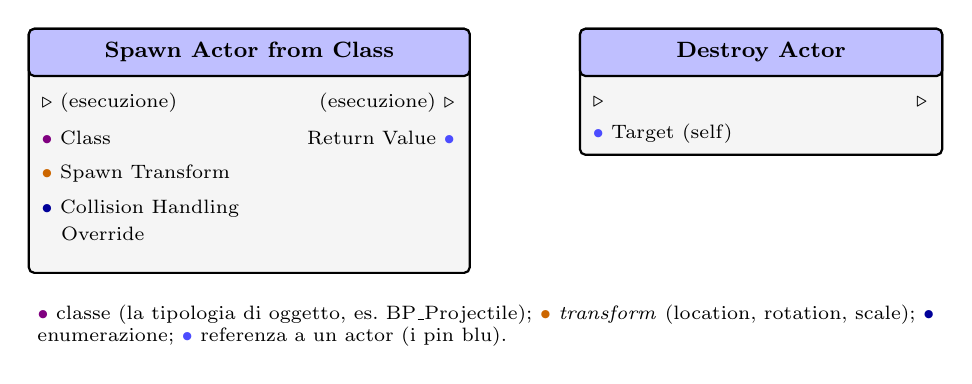
\begin{tikzpicture}[font=\footnotesize,
  ue5hdr/.style={draw, thick, fill=blue!25, minimum width=4.6cm, minimum height=0.6cm,
                 font=\footnotesize\bfseries, rounded corners=2pt},
  ue5bodyb/.style={draw, thick, fill=gray!8, minimum width=4.6cm, rounded corners=2pt},
  ue5pin/.style={font=\scriptsize, anchor=west},
  ue5pino/.style={font=\scriptsize, anchor=east}]
  % --- Spawn Actor from Class
  \node[ue5bodyb, minimum height=3.1cm, minimum width=5.6cm, anchor=north west] (sb)
    at (0,0) {};
  \node[ue5hdr, minimum width=5.6cm, anchor=north west] at (0,0) {Spawn Actor from
    Class};
  \node[ue5pin] at (0.05,-0.95) {$\triangleright$ (esecuzione)};
  \node[ue5pin] at (0.05,-1.4) {\textcolor{violet}{$\bullet$} Class};
  \node[ue5pin] at (0.05,-1.85) {\textcolor{orange!80!black}{$\bullet$} Spawn Transform};
  \node[ue5pin] at (0.05,-2.3) {\textcolor{blue!60!black}{$\bullet$} Collision Handling};
  \node[ue5pin] at (0.3,-2.62) {Override};
  \node[ue5pino] at (5.55,-0.95) {(esecuzione) $\triangleright$};
  \node[ue5pino] at (5.55,-1.4) {Return Value \textcolor{blue!70}{$\bullet$}};
  % --- Destroy Actor
  \node[ue5bodyb, minimum height=1.6cm, anchor=north west] at (7.0,0) {};
  \node[ue5hdr, anchor=north west] at (7.0,0) {Destroy Actor};
  \node[ue5pin] at (7.05,-0.95) {$\triangleright$};
  \node[ue5pin] at (7.05,-1.35) {\textcolor{blue!70}{$\bullet$} Target (self)};
  \node[ue5pino] at (11.55,-0.95) {$\triangleright$};
  % --- legenda
  \node[align=left, font=\scriptsize, anchor=north west, text width=11.4cm] at (0,-3.4)
    {\textcolor{violet}{$\bullet$} classe (la tipologia di oggetto, es.\ BP\_Projectile);
     \textcolor{orange!80!black}{$\bullet$} \emph{transform} (location, rotation,
     scale); \textcolor{blue!60!black}{$\bullet$} enumerazione;
     \textcolor{blue!70}{$\bullet$} referenza a un actor (i pin blu).};
\end{tikzpicture}
\caption{I due nodi della slide sullo spawn: in ingresso la classe da creare, il
\emph{transform} e il modo di gestire le collisioni; in uscita, la referenza all'actor
appena creato. Destroy Actor prende solo l'actor da distruggere. I colori dei pin
seguono le convenzioni dell'editor. Schema ricostruito.}
\label{ue5:fig:spawnnodes}
\end{figure}

\paragraph{Approfondimento: Collision Handling Override.} Il menù a tendina decide che
cosa fare se, nel punto di spawn, l'actor si troverebbe compenetrato con qualcos'altro.
Le opzioni sono: \emph{Default} (usa l'impostazione della classe), \emph{Always Spawn,
Ignore Collisions} (spawna comunque, anche dentro un muro), \emph{Try To Adjust
Location, But Always Spawn} (prova a spostarlo un poco, altrimenti spawna lì),
\emph{Try To Adjust Location, Don't Spawn If Still Colliding} (prova a spostarlo, e se
non trova posto non lo crea) e \emph{Do Not Spawn} (se c'è collisione, niente spawn).
Romero e Sewell (capitolo 3) suggeriscono anche di \textbf{promuovere a variabile} il
Return Value (tasto destro, \emph{Promote to Variable}) se l'oggetto creato servirà più
tardi, per esempio per distruggerlo; prima di usarla, la variabile va controllata con
un \textbf{Is Valid}, perché l'actor potrebbe essere già stato distrutto.

% ---------------------------------------------------------------------
\section{I cicli e il For Loop}
\label{ue5:sec:cicli}

``Anche un'altra cosa che andremo a vedere oggi sarà il \textbf{for loop}. Qualcuno ha
mai sentito parlare di \textbf{cicli} in programmazione?'' Uno studente che ha studiato
il C (``conosco \emph{while}, \emph{do while}, \emph{for}'') dà la definizione: ``è
ripetere un insieme di linee di codice finché una condizione è soddisfatta''. E fa un
esempio sulla torretta: ``finché il player sta in range della torretta, la torretta si
deve muovere; appena esce, quel codice non deve essere più ripetuto''. ``Sì,
assolutamente.''

Oggi, spiega il docente, si costruirà un actor che spawna dei cubetti ``in linea e in
colonne'': ``fondamentalmente andiamo a fare una \textbf{matrice}'', ``come in Excel,
ragazzi: le matrici per righe e colonne''. E lo si farà ``non uno per uno, ma tramite un
\textbf{indice}'': il For Loop è ``un modo iterativo di eseguire il codice fino a che
l'indice, quindi un numero che fa da dire OK, fatto il primo, OK, fatto il secondo, OK,
fatto il terzo\ldots{} Se arrivi a 10, smetti''. I cicli, infine, ``possono essere
innestati: cicli dentro altri cicli'', ed è esattamente ciò che servirà per righe e
colonne.

\paragraph{Approfondimento: i cicli dei Blueprint.} Nei Blueprint i cicli sono nodi di
\emph{flow control}. \textbf{For Loop} ha due ingressi interi, \textbf{First Index} e
\textbf{Last Index}, ed esegue il pin \textbf{Loop Body} una volta per ogni valore
dell'indice, dal primo all'ultimo \emph{compresi}, esponendo il valore corrente sul pin
\textbf{Index}; alla fine esegue \textbf{Completed}. \textbf{For Each Loop} fa lo stesso
scorrendo gli elementi di un array (Romero e Sewell, capitolo 13, lo usano per accendere
tutte le luci di una stanza). \textbf{While Loop} ripete finché una condizione booleana
è vera, come il \emph{while} del C. Una cosa importante, che distingue i cicli dei
Blueprint dal tempo del gioco: un For Loop si esegue \textbf{tutto nello stesso
\emph{frame}}, non ``piano piano nel tempo''. Non può contenere un Delay, e un ciclo
troppo lungo (o un While che non finisce mai) blocca il gioco; Unreal lo interrompe con
un errore di \emph{infinite loop} dopo un numero massimo di iterazioni. Per ripetere
qualcosa nel tempo si usano il Tick o i timer, come la torretta della quarta lezione.

% ---------------------------------------------------------------------
\section{Il fix della torretta: Find Relative Look at Rotation}
\label{ue5:sec:relative}

Prima dei proiettili, ``andremo a fissare una piccola cosa''. Il problema è quello visto
la volta scorsa: la torretta è fatta di tre \emph{static mesh}, e a ruotare è un solo
\emph{componente}, il Pivot, che ruota \textbf{rispetto al suo genitore}, la base. Find
Look at Rotation, invece, ``prenderà la rotazione in confronto a quella del
\textbf{mondo}, cioè di come è posizionato nel mondo''. Finché la torretta non è ruotata
nel livello le due cose coincidono; ma ``io giro la torretta a 90 gradi in engine, e poi
mi fa un offset di 90''.

\paragraph{La scoperta.} ``Ho scoperto, ed è una bellissima cosa, oserei dire, che Unreal
ci mette a disposizione il \textbf{Find Relative Look at Rotation} direttamente.'' Il
nodo ``prende il suo \emph{transform} e ci fa a quel punto un Find Look at Rotation in
relativa''. In pratica, in MoveTurret (il Custom Event chiamato dal timer):
\begin{itemize}
  \item si fa apparire \textbf{Find Relative Look at Rotation} al posto di Find Look at
        Rotation;
  \item al \textbf{Target} si collega quello che c'era già: la posizione del
        bersaglio, Get Actor Location di PlayerTarget;
  \item allo \textbf{Start Transform}, che chiede ``da che \emph{transform}
        partiamo'', si collega \textbf{Get Actor Transform} della torretta;
  \item l'uscita resta splittata, con la sola \textbf{Z} (lo \emph{yaw}) collegata al
        Target di \textbf{RInterp To}: ``questo non cambia assolutamente nulla''.
\end{itemize}
``Facendo ciò, da quel punto in poi la nostra torretta la possiamo ruotare come ci pare.
Tanto lui prenderà sempre a livello relativo.'' Il docente gira la torretta nel livello,
entra nel raggio: ``ecco che ci segue, senza cambiamenti, senza niente''
(figura~\ref{ue5:fig:relative}).

\paragraph{La velocità di interpolazione.} Il docente aveva trasformato l'Interp Speed in
una variabile e ``vi dico già che 0,01 era molto basso. Con questo find relative, ho
messo \textbf{2} e mi va più che bene. È anche più corretto''. A uno studente che non
sapeva come fosse nata la variabile: ``tira fuori dal pin, c'è scritto \emph{Promote to
Variable}''; poi si compila e, in basso a destra, nel \emph{Default Value}, si mette 2.
E, ``intanto'', il \textbf{Delta Time}: ``tira fuori dal Delta Time un pin e fai
\textbf{Get World Delta Seconds}''.

\begin{figure}[htbp]
\centering
\begin{tikzpicture}[font=\footnotesize,
  ue5node/.style={draw, thick, rounded corners=4pt, align=center, fill=gray!8,
                  minimum height=0.85cm, text width=2.4cm},
  ue5event/.style={ue5node, fill=red!12},
  ue5exec/.style={-{Stealth[length=2.5mm]}, very thick, black!80},
  ue5data/.style={-{Stealth[length=2mm]}, thick, blue!60!black},
  ue5trf/.style={-{Stealth[length=2mm]}, thick, orange!80!black},
  ue5flt/.style={-{Stealth[length=2mm]}, thick, green!50!black}]
  \node[ue5event] (mv) at (0,0) {\textbf{Custom Event}\\\textbf{MoveTurret}};
  \node[ue5node] (iv) at (3.1,0) {\textbf{Is Valid}\\PlayerTarget};
  \node[ue5node, text width=2.9cm] (srr) at (11.0,0) {\textbf{Set Relative
    Rotation}\\Target: Pivot};
  \draw[ue5exec] (mv) -- (iv);
  \draw[ue5exec] (iv) -- node[above, font=\scriptsize]{Is Valid} (srr);
  % dati
  \node[ue5node, fill=orange!12] (gat) at (0,-2.2) {\textbf{Get Actor
    Transform}\\(self)};
  \node[ue5node] (gal) at (0,-3.6) {\textbf{Get Actor Location}\\di PlayerTarget};
  \node[ue5node, text width=3.0cm, fill=yellow!20] (frl) at (3.6,-2.9)
    {\textbf{Find Relative Look at Rotation}\\Start Transform\\Target};
  \node[ue5node, text width=2.8cm] (ri) at (7.4,-2.9) {\textbf{RInterp To}\\
    Current: Get Relative Rotation (Pivot)\\Target: solo Z};
  \node[ue5node] (gwd) at (7.4,-5.0) {\textbf{Get World Delta Seconds}};
  \node[ue5node] (spd) at (4.1,-5.0) {\textbf{InterpSpeed}\\(variabile, 2)};
  \draw[ue5trf] (gat) -- (frl);
  \draw[ue5data] (gal) -- (frl);
  \draw[ue5flt] (frl) -- node[above, font=\scriptsize]{Z} (ri);
  \draw[ue5flt] (gwd) -- node[right, font=\scriptsize]{Delta Time} (ri);
  \draw[ue5flt] (spd) -- node[below, font=\scriptsize, pos=0.7]{Interp Speed} (ri);
  \draw[ue5flt] (ri.east) -| (srr.south);
\end{tikzpicture}
\caption{MoveTurret dopo il \emph{fix}. Il nodo nuovo (in giallo) calcola la rotazione
verso il bersaglio nello spazio della torretta, a partire dal suo \emph{transform}:
la torretta si può girare nel livello senza offset. Delta Time viene ora da Get World
Delta Seconds e l'Interp Speed, promosso a variabile, vale 2. Schema ricostruito.}
\label{ue5:fig:relative}
\end{figure}

\paragraph{Lo studente con la torretta che non gira.} Il primo caso in condivisione è
quello di uno studente che ha perso le lezioni precedenti per un problema al computer.
Il pivot non era stato reimportato a $-113$ (``non me l'ha fatto fare'', il re-import
non partiva). Lo si reimporta trascinando il file del materiale didattico nel
\emph{Content Browser} (attenzione a non lasciarlo cadere sopra altre cartelle); poi, in
scena, il pivot è ``storto'': lo si raddrizza con la modalità \textbf{Modeling}
(\textbf{Shift+5}), strumento \textbf{XForm}, \emph{Edit Pivot}. Nel Blueprint il pivot è
``un po' interrato'', e il cannone va staccato e riattaccato. Alla fine ruota, ``c'è un
piccolo offset, ma è importante che ruoti'', e punta ``dall'altra parte'': il caso è
rimandato alla pausa (sezione~\ref{ue5:sec:pausa}).

\paragraph{Approfondimento: perché il nodo nuovo risolve.} Find Relative Look at
Rotation (\emph{Start Transform}, \emph{Target Location}) trasforma prima il punto
bersaglio nello spazio locale del \emph{transform} di partenza, e poi calcola la
rotazione per guardarlo da lì. Il risultato è quindi già una rotazione
\textbf{relativa} all'actor, la stessa grandezza che Set Relative Rotation imposta sul
Pivot: i due spazi, che nel grafo della quarta lezione erano mescolati, ora coincidono.
Restano due avvertenze. Il punto di partenza è l'origine dell'actor, la base: va bene
per lo \emph{yaw}, ma per un \emph{pitch} preciso converrebbe partire dal
\emph{transform} del Pivot o del cannone (Get World Transform sul componente). E l'offset
dovuto alla \emph{mesh} reimportata a 113 gradi resta: il nodo presuppone che la
torretta, a rotazione zero, guardi lungo la propria X. Quanto alla velocità: con Delta
Time preso da Get World Delta Seconds e Interp Speed 2, il prodotto è circa 0,02 a 100
\emph{frame} al secondo, e la torretta insegue in modo morbido e uguale su ogni
macchina, come anticipato nella lezione precedente.

% ---------------------------------------------------------------------
\section{I trace: linee immaginarie}
\label{ue5:sec:trace}

``Abbiamo parlato di spawn, ma anche una cosa che andremo a vedere è chiamata
\textbf{line trace}.'' ``Oggi usiamo lo \textbf{sphere trace}, però in generale un trace
è una \textbf{linea immaginaria} che viene fatta dall'engine'' per scoprire che cosa c'è
lungo un percorso.

\paragraph{La dimostrazione.} Il docente lo mostra con la torretta che aveva già
preparato (``ecco qua, spawnano la marea di proiettili''). Entrando nel raggio, davanti
al cannone compare un \textbf{reticolo rosso}: ``una linea immaginaria, che non vedremo
se dovessimo avere un eseguibile''. Ma ``vedete che è rosso, rosso, rosso; se
\emph{overlappa}, diventa \textbf{verde}. Dice: ah, ho visto qualcosa! E quindi comincia
a sparare''. Poi, per confronto, trasforma al volo lo sphere trace in un \textbf{Line
Trace by Channel}: ``facciamo una linea''. All'inizio la linea non trova nulla, ``perché
è impostata male''; basta cambiarle il canale, e ``ecco che ci ha trovato'': ``fa rosso
il puntino e verde. Dice: ah, ok, ti ho beccato''.

\paragraph{A che cosa servono.} ``Sono delle linee immaginarie che servono a noi
\emph{developer} per dire: oh, c'è qualcosa che overlappa una linea invisibile?
Effettivamente sì, effettivamente no.'' Il docente racconta di averle usate per
un'intelligenza artificiale: ``tracciavo una linea tra me e il player; se c'era qualcosa
di mezzo, vuol dire che non lo vedeva; se invece non c'era niente, vuol dire che lo
vedeva''. È ``proprio una \textbf{linea di vista}''. E un avvertimento, ripetuto:
``non esagerate con il trace, perché anche esso è molto pesante'', tanto più se, come
oggi, lo si fa a ogni \emph{frame}.

\paragraph{Approfondimento: le famiglie di trace.} Romero e Sewell (capitolo 14)
definiscono i trace come test di collisione lungo un segmento. Ne esistono di due
tipi di ``filtro'': \textbf{by Channel}, che cercano gli oggetti che bloccano un
\emph{trace channel} (Visibility, Camera o un canale creato da noi), e \textbf{for
Objects}, che cercano gli oggetti di certi \emph{object type} (WorldStatic,
WorldDynamic, Pawn, PhysicsBody, Vehicle, Destructible). E di quattro forme: la
\textbf{linea}, la \textbf{sfera}, la \textbf{capsula} e il \textbf{box}, dove le forme
``spesse'' sono più costose della linea. Infine, ogni trace ha una versione singola,
che restituisce il primo oggetto colpito, e una \textbf{Multi}, che li restituisce
tutti (sezione~\ref{ue5:sec:errori}). Tutti hanno gli stessi ingressi principali:
\textbf{Start} ed \textbf{End}, il canale o i tipi, \textbf{Trace Complex} (testare
contro la \emph{mesh} vera o contro le forme di collisione semplificate), \textbf{Actors
to Ignore}, \textbf{Draw Debug Type} e \textbf{Ignore Self}. Le uscite sono un
\textbf{Out Hit} (una struttura \emph{Hit Result} con, tra l'altro, il punto d'impatto,
la normale della superficie e l'actor colpito, leggibili con \emph{Break Hit Result}) e
un \textbf{Return Value} booleano: vero se qualcosa ha bloccato il trace.

% ---------------------------------------------------------------------
\section{L'evento Shoot e i vettori del trace}
\label{ue5:sec:shoot}

``La prima cosa è che dobbiamo creare un evento \textbf{Shoot}'': un \textbf{Custom
Event} nel grafo di BP\_Turret.

\paragraph{Is Valid, per buona maniera.} ``Intanto la prima cosa che andiamo a fare è
vedere se esiste il target'': un \textbf{Is Valid} (``la macro con il punto
interrogativo'') su PlayerTarget. ``È buona maniera fare questa cosa, di vedere se
effettivamente esiste o non esiste, perché ci ottimizza i processi'': se non c'è un
bersaglio, non si esegue nulla. (Più avanti, nella sezione~\ref{ue5:sec:bocche}, questo
Is Valid verrà spostato fuori da Shoot.)

\paragraph{Lo Sphere Trace by Channel.} Poi lo \textbf{Sphere Trace by Channel}: ``una
linea immaginaria che andremo a creare in modo tale che, se il nostro character entra in
questa sfera, vuol dire che io lo sto vedendo ed è in puntamento''. Che cosa chiede?
``Un punto di \textbf{Start} e un punto di \textbf{End}'', con i pin
\textbf{gialli}. ``Chi si ricorda quali sono gli elementi gialli in Unreal?'' ``Un
vettore.'' ``Bravissimo, è un vettore. In questo caso, un vettore di locazione'': una X,
una Y e una Z.

\paragraph{Il punto di partenza: TraceSpawn.} Il trace deve partire ``più o meno dalla
canna, da questo punto qua in avanti''. Si potrebbe usare la posizione del Pivot, ``però
vi dico che è più corretto fare una cosa del genere: andiamo a creare proprio un
\textbf{punto vuoto}'' dedicato. Nei componenti si fa \emph{Add} e si scrive
\textbf{Scene}: un \emph{Scene Component}, ``solo un punto nello spazio'', senza
\emph{mesh} né collisioni. Lo si \textbf{attacca al cannone}, lo si posiziona ``in
mezzo alle due canne'', e lo si rinomina (``per rinominare le cose molto più
velocemente: cliccate sull'elemento, \textbf{F2}, e scrivete'') in
\textbf{TraceSpawn}. ``L'abbiamo attaccato al cannone perché il pivot fa ruotare il
cannone e il cannone farà ruotare il TraceSpawn: c'è questa \textbf{dipendenza a
cascata}.'' Dal componente TraceSpawn si prende \textbf{Get World Location}, ``dove è
posizionato nel mondo'', e la si collega allo \textbf{Start}.

\paragraph{Il punto d'arrivo: il forward vector.} ``Ci manca quello del punto di fine.
Dove deve arrivare?'' Qui torna la teoria dei vettori della quarta lezione. Ogni
\emph{mesh}, ogni componente, ogni actor ha dei vettori di direzione ``già prefatti'':
\begin{itemize}
  \item \textbf{Get Actor Forward Vector}, che ``punterà sempre in avanti'';
  \item \textbf{Get Actor Right Vector}, ``che punterà sempre a destra'';
  \item \textbf{Get Actor Up Vector}, ``che punterà sempre in alto'',
\end{itemize}
sempre relativi all'oggetto. ``Domanda: se io moltiplicassi per $-1$ il forward vector,
dove punterà rispetto alla mesh?'' ``Dietro.'' ``Bravissimo'': moltiplicare per $-1$
``inverte il risultato''; così si ottengono il \emph{back} vector, la sinistra e il
basso.

\paragraph{Lungo 1: moltiplicare.} Ma se si collega il forward vector così com'è ``non ci
darà assolutamente nulla, perché è molto piccolo'': ``il forward vector che ci dà Unreal
è di \textbf{lunghezza 1}'', un vettore normalizzato. ``Buona prassi è prenderlo e
moltiplicarlo, per esempio per \textbf{800}'': ``avremo un vettore 800 volte più
lungo''. (Uno studente non riesce a scrivere 800 nel Multiply: ``il pallino è giallo e
non verde''. ``Se moltiplicate un vettore, vi dà direttamente la moltiplicazione per un
altro vettore, ma potete cambiare il secondo fattore: tasto destro, \emph{To Float}.
Diventerà verde, e ci mettete 800.'')

\paragraph{Un punto non è una linea: sommare.} ``Magari vi verrebbe da dire: ok, ho
trovato il punto laggiù, lo vado a mettere nell'End. No, ancora no.'' Il forward vector
moltiplicato è ``un punto, non è una linea'': è uno spostamento di 800 in avanti,
calcolato come se si partisse dall'origine del mondo. ``Per farlo diventare una linea
dobbiamo letteralmente \textbf{sommare} due vettori'': la World Location di TraceSpawn
più il forward vector per 800. ``È un discorso che sembra strano, però effettivamente
quello che abbiamo qua è solo un punto nello spazio; con la somma ne traiamo un'effettiva
linea'' (figura~\ref{ue5:fig:vettori}).

\paragraph{Il forward vector giusto.} Alla prima prova il trace c'è, ma ``non segue il
pivot'': resta fermo mentre la torretta ruota. Il motivo: Get \emph{Actor} Forward
Vector è il vettore dell'actor intero, cioè della \textbf{base}, ``quindi sarà sempre lì.
Non girerà, perché deve girare insieme al cannone''. La correzione: ``invece di prendere
il Get Actor Forward Vector, prendiamo il \textbf{Get Forward Vector del TraceSpawn}''.
(``A me non fa collegare TraceSpawn e Get Forward Vector'': bisogna tirare il filo
\emph{dal} componente TraceSpawn e cercare \emph{Get Forward Vector}, la versione per i
componenti.)

\begin{figure}[htbp]
\centering
\begin{tikzpicture}[font=\footnotesize, >={Stealth[length=2.5mm]}]
  % assi del mondo
  \draw[->, thick, gray] (-0.3,0) -- (2.0,0) node[right]{X};
  \draw[->, thick, gray] (0,-0.3) -- (0,1.8) node[above]{Y};
  \node[below left, gray, font=\scriptsize] at (0,0) {origine del mondo};
  % torretta vista dall'alto
  \coordinate (C) at (6.0,0.4);
  \fill[gray!25, draw=black, thick] (C) circle (0.7);
  \node[font=\scriptsize, below] at ($(C)+(0,-0.7)$) {base};
  \begin{scope}[rotate around={35:(C)}]
    \fill[orange!25, draw=black, thick] ($(C)+(0,-0.2)$) rectangle ($(C)+(1.3,0.2)$);
  \end{scope}
  \coordinate (S) at ($(C)+(35:1.15)$);
  \fill[blue!60] (S) circle (0.07);
  \node[font=\scriptsize, align=center] at ($(S)+(-0.9,0.55)$) {TraceSpawn\\(Start)};
  % vettore posizione
  \draw[->, very thick, blue!60!black] (0,0) -- (S) node[pos=0.45, below, sloped,
    font=\scriptsize] {Get World Location};
  % forward unitario all'origine
  \draw[->, very thick, red!70!black] (0,0) -- (35:0.8);
  % forward x 800 all'origine (punto sbagliato)
  \draw[->, thick, red!70!black, dashed] (0,0) -- (35:3.6);
  \fill[red!70!black] (35:3.6) circle (0.06);
  \node[red!70!black, font=\scriptsize, align=left, anchor=south east] at (35:3.6)
    {Forward $\times$ 800\\(da solo: un punto\\vicino all'origine)};
  \node[red!70!black, font=\scriptsize, anchor=north west] at (0.15,-0.25)
    {Forward: lunghezza 1};
  % fine = start + forward x 800
  \coordinate (E) at ($(S)+(35:3.6)$);
  \draw[->, very thick, green!45!black] (S) -- (E);
  \fill[green!45!black] (E) circle (0.07);
  \node[right=3pt, green!45!black, align=left] at (E) {End =\\Start + Forward
    $\times$ 800};
  % sfera del trace
  \foreach \t in {0.2,0.45,0.7,0.95} {
    \draw[green!45!black, thin] ($(S)!\t!(E)$) circle (0.32);
  }
  \node[green!45!black, font=\scriptsize, anchor=west] at ($(S)!0.5!(E)+(0.45,-0.3)$)
    {Sphere Trace, Radius 80};
\end{tikzpicture}
\caption{I vettori del trace, visti dall'alto. Get World Location di TraceSpawn è un
vettore dall'origine del mondo al punto di partenza. Il Forward Vector è lungo 1;
moltiplicato per 800 diventa uno spostamento, che però, preso da solo, indica un punto
vicino all'origine (tratteggio). Sommato alla posizione di partenza, dà la fine giusta:
800 unità davanti alla canna. Lo sphere trace ``trascina'' una sfera di raggio 80 lungo
il segmento. Schema ricostruito, non in scala.}
\label{ue5:fig:vettori}
\end{figure}

\paragraph{Il raggio e il debug.} Due dettagli ancora. Il \textbf{Radius} dello sphere
trace parte da zero: ``il raggio della nostra bellissima sfera sarà zero, quindi non
esisterà''. Il docente mette \textbf{80}. E per vedere il trace in editor, ``lo vedremo
solo noi \emph{developer}'', c'è \textbf{Draw Debug Type}, da impostare su \textbf{For
One Frame}: ``perché se adesso la mettiamo \emph{For Duration}, ha una durata, sarà un
casino, perché lo fa ogni \emph{frame}'' (tabella~\ref{ue5:tab:debug}). Per provarlo,
Shoot viene chiamato dall'\textbf{Event Tick} (``prendete il Tick, scrivete Shoot,
come avete chiamato questo evento''): ``giusto per vedere effettivamente che
funzioni''.

\begin{table}[htbp]
\centering
\small
\begin{tabular}{@{}p{3.0cm}p{11.0cm}@{}}
\toprule
\textbf{Draw Debug Type} & \textbf{Che cosa disegna} \\
\midrule
None & niente: il trace c'è, ma non si vede (il valore di default) \\
For One Frame & il trace per un solo \emph{frame}: se il trace è chiamato a ogni
\emph{frame}, si vede ``in diretta''; è l'opzione usata a lezione \\
For Duration & il trace resta visibile per un certo tempo (Draw Time, nei dettagli del
nodo): chiamato a ogni \emph{frame}, accumula centinaia di disegni sovrapposti \\
Persistent & il trace resta disegnato per sempre: utile per un trace singolo, da
esaminare con calma \\
\bottomrule
\end{tabular}
\caption{Le opzioni di Draw Debug Type dei nodi di trace. I colori del disegno sono il
rosso per il tratto libero e il verde dal punto in cui il trace è stato bloccato (Trace
Color e Trace Hit Color, modificabili nel nodo).}
\label{ue5:tab:debug}
\end{table}

\paragraph{I problemi del momento.} Le condivisioni mostrano errori ricorrenti: lo
Start e l'End scambiati o collegati senza la somma (``Start è questo, solo questo; lo
attacchi così; il più va nell'End''); Draw Debug Type lasciato su \emph{None}; Shoot non
chiamato dal Tick (``l'hai messo sul Tick? Ah, no. Metti l'evento Shoot sul Tick''); e
la linea che compare ma non ruota con il cannone, per il motivo visto sopra.

% ---------------------------------------------------------------------
\section{I trace channel e le risposte di collisione}
\label{ue5:sec:canali}

Ora il trace c'è e ruota, ``ma come potete vedere non abbiamo il verdino, non ci dice
\emph{ho trovato}'': il player ci passa attraverso senza essere visto. Il motivo è il
\textbf{trace channel}. ``Di standard Unreal ci dà due canali, che sono
\textbf{Visibility} e \textbf{Camera}''; quello del docente (``questo qua al testo lo
vedete, l'ho creato io'') è un canale \textbf{custom}, che risponde ``in una certa
maniera, dipendentemente da certe opzioni''. Bisogna crearlo.

\paragraph{Creare il canale.} Dal menù \textbf{Edit}, \textbf{Project Settings}; si scende
``giù giù giù giù'' fino a \textbf{Collision} (nella sezione \emph{Engine}). Lì,
\textbf{New Trace Channel}: ``lo chiamate come volete, lo chiamiamo magari
\textbf{DetectionTurret}'', con \textbf{Default Response} su \textbf{Ignore}. Che cosa
vuol dire? ``Guarda questo trace: in risposta a tutti gli altri elementi in cui può
collidere, cosa fa di base? Ignora tutto, perché è meglio che ignori tutto, in modo tale
che tanto deve trovare solo il player.'' Se si mettesse \emph{Block}, ``ci bloccherebbe
tutto quanto'', e bisognerebbe togliere il blocco a tutti gli elementi statici e
dinamici. ``È più facile mettere ignora tutto, e poi mettiamo il \emph{tick} positivo al
nostro player.''

\paragraph{Il player risponde Block.} Si apre il \textbf{Third Person Character}, si
seleziona la \textbf{Mesh} e si cerca \emph{Collision} nei dettagli (``importante che, se
non avete compilato, compilate, perché se no non vi apparirà mai il nostro
DetectionTurret''). I \textbf{Collision Presets} sono grigi, perché è attivo un
\emph{preset}: si sceglie \textbf{Custom} dalla tendina, e nella riga di DetectionTurret
si mette la spunta su \textbf{Block}. ``In che modo reagisci al trace channel della
nostra torretta? Overlap, Block, Ignore. In questo caso andiamo a fare che blocca.''

\paragraph{Ignore, Overlap, Block.} Il docente ripassa le tre risposte con le mani:
``questa è la mia mano, l'oggetto 1, l'oggetto 2''. Con l'\textbf{Overlap}, ``se si
toccano non c'è una collisione fisica, quindi volendo si trapassano'', ma ``c'è una
\emph{detection}: l'engine dice, sono loro che collidono, quindi c'è un segnale''; è ciò
che si usa ``per i blocchi invisibili''. Il \textbf{Block}, invece, ``è proprio un
blocco fisico''. Il trace non ha un corpo, quindi per lui il Block è ``semplicemente
un'accortezza'': ``ehi, ho trovato il player, mi blocco''; ed è grazie al blocco che
appare la sfera ``parte verde, parte rossa'' (tabella~\ref{ue5:tab:risposte}).

\begin{table}[htbp]
\centering
\small
\begin{tabular}{@{}p{2.0cm}p{5.6cm}p{6.4cm}@{}}
\toprule
\textbf{Risposta} & \textbf{Tra due corpi} & \textbf{Per un trace} \\
\midrule
Ignore & si attraversano e nessuno se ne accorge & l'oggetto è invisibile per quel
trace \\
Overlap & si attraversano, ma scatta un evento di \emph{overlap} (i ``blocchi
invisibili'', la sfera della torretta) & il trace lo registra ma prosegue: lo vede solo
un trace Multi, e il Return Value resta falso \\
Block & si fermano l'uno contro l'altro: collisione fisica & il trace si ferma lì: è un
\emph{hit}, il disegno di debug diventa verde e il Return Value è vero \\
\bottomrule
\end{tabular}
\caption{Le tre risposte di collisione. Ogni componente dichiara una risposta per ogni
canale (Visibility, Camera, i canali custom) e per ogni \emph{object type}; quando due
oggetti si incontrano, vale la risposta più ``debole'' delle due.}
\label{ue5:tab:risposte}
\end{table}

\paragraph{Scegliere il canale nel trace.} Tornati in BP\_Turret, nello Sphere Trace by
Channel di Shoot si apre la tendina \textbf{Trace Channel}: ``c'è Visibility, Camera e
DetectionTurret''. Se compaiono solo Visibility e Camera, ``vai con \textbf{Compile},
qui in alto a sinistra''. In Play: ``vedete che è diventato verde. C'è il trace rosso,
viene bloccato, e da lì in poi c'è quello spazio verde'': ``è da lì in poi che il nostro
player è presente''. Avvicinandosi, il tratto verde si allunga.

\paragraph{Il Return Value.} Infine un \textbf{Print String} collegato al
\textbf{Return Value} del trace, ``che ci dice letteralmente: hai preso qualcosa? Sì,
no''. È un \textbf{booleano}: falso se non ha trovato niente, vero se ha trovato
qualcosa. In Play ``spunteranno un botto di true e false, ma è normale, sta sul Tick'':
``false, false, false\ldots{} true, true, true''.

\paragraph{Approfondimento: Mesh o Capsule?} A lezione la risposta Block al canale
DetectionTurret viene data alla \textbf{Mesh} del personaggio, e funziona. Nel Third
Person Character, però, il componente che rappresenta il corpo ai fini delle collisioni
è la \textbf{Capsule Component}, la radice; la Mesh scheletrica, di default, usa un
\emph{preset} (\emph{CharacterMesh}) pensato per non interferire con il movimento. Dare
il Block alla Mesh significa che il trace colpisce la forma del personaggio, con le sue
parti fisiche; darlo alla capsula significa colpire un cilindro più semplice. Entrambe
le scelte sono legittime; l'importante è sapere quale si è fatta, perché l'\emph{Hit
Actor} sarà lo stesso, ma l'\emph{Hit Component} e il punto d'impatto no.

% ---------------------------------------------------------------------
\section{Il proiettile: BP\_Projectile e il Projectile Movement}
\label{ue5:sec:proiettile}

``Abbiamo fatto la torretta che gira, abbiamo fatto la torretta che detecta: adesso
dobbiamo far sparare.'' Un Custom Event \textbf{SpawnProjectile}, ``ma che succede,
ragazzi? Non abbiamo un proiettile''. Lo si crea: tasto destro nel Content Browser,
\textbf{Blueprint Class}, \textbf{Actor}, e lo si chiama \textbf{BP\_Projectile}.

\paragraph{Due actor, due compiti.} Perché un Blueprint a parte, e non tutto dentro la
torretta? ``Due actor, uno che fa un compito e uno che fa un altro, è il miglior modo
per gestire i comportamenti.'' ``Perché a un certo punto magari vi arriva un
\emph{designer} e vi dice: ragazzi, non voglio che spawni più i proiettili, voglio che
spawni \textbf{banane}. Eh, se l'avete fatto dentro la torretta dovete fare un casino.
Invece, cambiare semplicemente il proiettile è molto più facile.''

\paragraph{La mesh.} Il proiettile è ``formato da due cose''. La prima è una \textbf{Static
Mesh}, rinominata \textbf{MeshProjectile}: una \textbf{sfera} di default (``se volete,
potete scaricare un modello, così ci mettete un proiettile al posto della palla'').
La si scala a \textbf{0,5}, poi a \textbf{0,3} (``mi sembra un po' grandicello''),
con il \textbf{lucchetto} della scala chiuso. ``Questo lucchetto l'abbiamo spiegato alla
prima lezione'': aperto, permette di modificare gli assi uno per uno; chiuso, ``se
modificate un singolo asse, vi scalerà anche le altre, in modo tale che rimangano
uniformi, perché sennò vengono forme stiracchiate''. Come materiale, \textbf{MI\_Solid\_Blue}
(``mi solid blue'').

\paragraph{Il Projectile Movement.} La seconda cosa è il movimento. ``Unreal ci arriva
con un regalo incredibile'': come la volta scorsa c'era il Rotating Movement per il
mulino, ``arriva la possibilità di avere un \textbf{Projectile Movement}, per quanti
giochi ormai hanno dei proiettili''. Si aggiunge il componente, e nei dettagli ci sono
``un sacco di dati in cui possiamo giocare'': ``tanti giochi ai giorni d'oggi hanno cose
molto comuni. Quanti FPS ce ne sono? Anche le armi di \emph{Borderlands}, che sono tutte
strane, alla base si parla sempre di sparare''. I valori della lezione:
\begin{itemize}
  \item \textbf{Initial Speed} 1000 e \textbf{Max Speed} 1000 (per guardarlo meglio, a
        un certo punto l'Initial Speed scende a 100, ``la lumaca'', e poi torna a 1000,
        ``una velocità da proiettile'');
  \item \textbf{Projectile Gravity Scale} a \textbf{0}: ``questo proiettile al momento
        è afflitto dalla gravità''; ``noi vogliamo che vada dritto per dritto'';
  \item \textbf{Velocity} lasciata a $(1, 0, 0)$: ``la velocità è la direzione'',
        quindi ``è 1 sull'asse X'', e il proiettile ``andrà dritto così''.
\end{itemize}
E la mesh deve essere \textbf{Movable}, ``se no vi danno errore''. Messo in scena e
avviato il Play, ``il nostro bellissimo proiettilino se ne va per la sua'' strada:
attraversa tutto, ``overlapperà, e chissà chi lo vedrà più''. (A una studentessa la
pallina ``cade semplicemente'': aveva lasciato la gravità a 1.)

\paragraph{Approfondimento: i parametri del Projectile Movement.} Romero e Sewell
(capitolo 6) modificano il proiettile del modello \emph{First Person} con gli stessi
parametri. \textbf{Initial Speed} è la velocità con cui il proiettile parte; \textbf{Max
Speed} è il limite, che conta solo se qualcos'altro lo accelera (un razzo con il motore
acceso); per un proiettile d'arma ha senso che le due coincidano. \textbf{Velocity} è
una direzione nello spazio \emph{locale} del proiettile: se Initial Speed è maggiore di
zero, Unreal ne usa solo la direzione e la moltiplica per l'Initial Speed. Per questo
è importante che lo spawn dia al proiettile la rotazione giusta: la X locale del
proiettile deve guardare fuori dalla canna. \textbf{Projectile Gravity Scale} moltiplica
la gravità del mondo (0 nessuna, 0,1 ``proiettile leggero''). La sezione \textbf{Projectile
Bounces}, con \emph{Should Bounce}, decide se rimbalza sui muri; e \textbf{Rotation Follows
Velocity} lo fa girare nella direzione del moto, utile per frecce e razzi.

% ---------------------------------------------------------------------
\section{Il proiettile che si distrugge}
\label{ue5:sec:distruzione}

``Noi vorremmo che il nostro proiettile sia molto più realistico: trova un muro e
scompare.'' E non è solo estetica: ``immaginatevi che adesso spawneremo dei proiettili
che andranno nell'infinito e oltre''; l'engine ``dirà: guarda, esiste'', e ``non
libereremo mai la memoria''.

\paragraph{Un trace attorno al proiettile.} La soluzione riusa il trace: nell'\textbf{Event
Tick} di BP\_Projectile, uno \textbf{Sphere Trace by Channel} di raggio \textbf{30},
``una sfera intorno al nostro proiettile che ci dirà: guarda, hai colpito qualcosa?''.
Start ed End sono \textbf{lo stesso punto}, \textbf{Get Actor Location} del proiettile:
``vogliamo che l'inizio e la fine siano lo stesso punto''. Con Draw Debug Type su For
One Frame, ``intorno alla nostra pallina si è creato un trace''.

\paragraph{Branch e Destroy Actor.} Poi: ``molto semplicemente, Return Value è vero? Sì?
Allora distruggete''. Un \textbf{Branch} (``tenete premuto B e cliccate'') sul Return
Value, e sul ramo True un \textbf{Destroy Actor} (figura~\ref{ue5:fig:proiettile}). In
Play, alla ``velocità della lumaca'', il proiettile arriva al muro e sparisce: ``si è
distrutto, quindi abbiamo il comportamento di base''. Il Tick, nota il docente,
``inizierà solamente quando l'oggetto esiste'': ogni proiettile controlla sé stesso
finché vive.

\begin{figure}[htbp]
\centering
\begin{tikzpicture}[font=\footnotesize,
  ue5node/.style={draw, thick, rounded corners=4pt, align=center, fill=gray!8,
                  minimum height=0.85cm, text width=2.5cm},
  ue5event/.style={ue5node, fill=red!12},
  ue5exec/.style={-{Stealth[length=2.5mm]}, very thick, black!80},
  ue5vec/.style={-{Stealth[length=2mm]}, thick, yellow!50!black},
  ue5bool/.style={-{Stealth[length=2mm]}, thick, red!60!black},
  ue5comp/.style={draw, thick, rounded corners=3pt, minimum width=3.5cm,
                  minimum height=0.55cm, align=center, font=\scriptsize}]
  % componenti
  \node[font=\scriptsize\bfseries] at (0,1.0) {BP\_Projectile: componenti};
  \node[ue5comp, fill=gray!20] (r) at (0,0.4) {DefaultSceneRoot};
  \node[ue5comp, fill=blue!20] (m) at (0.6,-0.3) {MeshProjectile (sfera, 0,3)};
  \node[ue5comp, fill=green!15] (pm) at (0,-1.0) {ProjectileMovement};
  \draw[thick, gray!60!black] ([xshift=-1.5cm]r.south) |- (m.west);
  \node[font=\scriptsize, align=left, anchor=west] at (-1.45,-1.75)
    {Initial / Max Speed 1000\\Gravity Scale 0, Velocity (1,0,0)};
  % grafo
  \node[ue5event] (tick) at (4.4,0.2) {\textbf{Event Tick}};
  \node[ue5node, text width=3.0cm] (st) at (7.9,0.2) {\textbf{Sphere Trace by
    Channel}\\Radius 30\\Channel: ProjectileTrace\\Debug: For One Frame};
  \node[ue5node, text width=1.6cm] (br) at (11.3,0.2) {\textbf{Branch}};
  \node[ue5node, text width=1.9cm] (de) at (11.3,-1.9) {\textbf{Destroy Actor}\\(self)};
  \node[ue5node] (gal) at (4.4,-1.6) {\textbf{Get Actor Location}\\(self)};
  \draw[ue5exec] (tick) -- (st);
  \draw[ue5exec] (st) -- (br);
  \draw[ue5exec] (br) -- node[right, font=\scriptsize]{True} (de);
  \draw[ue5vec] (gal.east) -| node[pos=0.75, left, font=\scriptsize, align=right]
    {Start\\e End} (st.south);
  \draw[ue5bool] ([yshift=-0.4cm]st.east) -- node[above, font=\scriptsize, pos=0.4]
    {Return Value} ([yshift=-0.4cm]br.west);
\end{tikzpicture}
\caption{Il proiettile. A sinistra i componenti: una sfera scalata e il Projectile
Movement, che fa tutto il moto. A destra il grafo: a ogni \emph{frame}, una sfera di
raggio 30 attorno al proiettile (Start ed End coincidono); se qualcosa la blocca, il
proiettile si distrugge. Il canale, all'inizio Visibility e poi Camera, diventa alla
fine ProjectileTrace. Schema ricostruito.}
\label{ue5:fig:proiettile}
\end{figure}

\paragraph{Approfondimento: altri modi di distruggere un proiettile.} Il trace sul Tick
funziona ed è istruttivo, ma non è l'unico modo, né il più economico. Il Projectile
Movement ha un proprio evento, \textbf{On Projectile Stop}, che scatta quando il
proiettile si ferma contro qualcosa che lo blocca; e un componente di collisione (una
Sphere Collision come radice del proiettile, con il Projectile Movement che la muove)
genera \textbf{Event Hit} o \textbf{On Component Hit} all'impatto. Romero e Sewell
(capitolo 6) collegano proprio all'evento di \emph{hit} il Destroy Actor, ``così che il
proiettile venga sempre distrutto quando collide''. Infine, per i proiettili che non
colpiscono nulla, l'actor ha una proprietà \textbf{Initial Life Span} (nei \emph{Class
Defaults}): se maggiore di zero, l'actor si distrugge da solo dopo quei secondi. È una
rete di sicurezza contro i proiettili che vanno ``nell'infinito e oltre''.

% ---------------------------------------------------------------------
\section{Visibility, Camera e il canale ProjectileTrace}
\label{ue5:sec:projtrace}

Il proiettile si distrugge contro il muro, ``anche il player, volendo?'' No: ``mi metto
davanti, e infatti non ce lo prende''. Con il canale \textbf{Visibility} il personaggio
non viene visto; cambiando il canale in \textbf{Camera}, ``così ci prende pure il
player''.

\paragraph{Perché.} Il docente apre le collisioni del Third Person Character: c'è la
tabella delle \textbf{Collision Responses}, con Ignore, Overlap e Block, e sotto le
\textbf{Trace Responses}, ``cioè come rispondo a questo trace''. ``Come rispondo al trace
Visibility? Vedete che c'è la spunta su Ignore; invece il Camera viene bloccato.''
``Semplicemente è un concetto di collisioni.''

\paragraph{Un canale per il proiettile.} ``Lo facciamo, ragazzi, così almeno è buona
prassi'': un secondo canale, \textbf{ProjectileTrace}. Qui il ragionamento è opposto a
quello di DetectionTurret. Il docente prima pensa a Ignore e a mettere il Block sui
quattro muri uno per uno (``però è più pesante''), poi cambia idea: ``è molto meglio
farlo in \textbf{Block}, così facciamo un Block e leviamo semplicemente quelli che non ci
interessano''. La regola generale: ``quante cose ho che devono bloccare, e quante che
devono ignorare?''. Il proiettile ``sbatte praticamente con tutto'', quindi Default
Response \textbf{Block}, e si escludono le poche eccezioni (tabella~\ref{ue5:tab:canali}):
\begin{itemize}
  \item il \emph{character}: Block (``va benissimo'');
  \item la \textbf{Sphere} della torretta, il raggio d'azione: Custom, ProjectileTrace
        su \textbf{Ignore}, altrimenti il proiettile esploderebbe appena nato, dentro la
        sfera;
  \item anche \textbf{Pivot}, \textbf{Base} e \textbf{Cannon}: ``non vogliamo che
        rimbalzi contro la stessa torretta che l'ha sparato'', quindi Custom e Ignore
        a tutti e tre.
\end{itemize}
Nel trace del proiettile si sceglie ProjectileTrace (``sempre compilato, perché se no non
vi arriva''), e in Play il proiettile si distrugge sia sul player sia sul muro.

\begin{table}[htbp]
\centering
\small
\begin{tabular}{@{}p{2.8cm}p{2.1cm}p{9.1cm}@{}}
\toprule
\textbf{Canale} & \textbf{Default} & \textbf{Eccezioni impostate a lezione} \\
\midrule
DetectionTurret & Ignore & Mesh del Third Person Character: \textbf{Block}. Il trace
della torretta vede solo il giocatore. \\
ProjectileTrace & Block & Sphere, Pivot, Base e Cannon della torretta: \textbf{Ignore};
dopo la pausa anche la sfera del proiettile stesso. Character: Block. Il proiettile si
ferma su tutto tranne che sulla torretta che lo spara. \\
\bottomrule
\end{tabular}
\caption{I due \emph{trace channel} creati in Project Settings $\rightarrow$ Engine
$\rightarrow$ Collision. Il principio: se le cose da colpire sono poche, Default
Ignore e Block sulle eccezioni; se sono molte, Default Block e Ignore sulle eccezioni.}
\label{ue5:tab:canali}
\end{table}

\paragraph{``A me passa attraverso.''} Due studenti hanno il proiettile che attraversa
player e muri (``il player me lo sposta, e i muri li attraversa''). Si controllano il
canale (Block), il nodo (ProjectileTrace), le collisioni della Mesh: tutto giusto. Il
colpevole è il \textbf{Radius}: ``era zero, quindi era invisibile''. ``Attenzione,
ragazzi, perché il radius è la grandezza: se è zero, non esiste.'' (E il raggio del
trace della torretta? ``80.'') Un'altra studentessa non trova i Collision Presets della
Sphere della torretta: bisogna selezionare proprio il componente \emph{Sphere} nella
lista dei componenti, e la sezione Collision compare.

\paragraph{Approfondimento: Ignore Self e Actors to Ignore.} Tutti i nodi di trace hanno
la casella \textbf{Ignore Self}, attiva di default: il trace ignora tutti i componenti
dell'actor che lo esegue. Il trace del proiettile, quindi, non vede la propria sfera
anche senza toccarne le collisioni, e quello della torretta non vede la torretta. Per
escludere \emph{altri} actor, senza modificare le loro collisioni, c'è l'ingresso
\textbf{Actors to Ignore}, un array: per esempio, il proiettile potrebbe ricevere allo
spawn una referenza alla torretta che l'ha sparato (i pin \emph{Owner} e \emph{Instigator}, che compaiono espandendo
Spawn Actor from Class, servono proprio a passare questo genere di informazione) e ignorarla nel trace. È la soluzione più pulita quando le torrette sono tante e
ognuna deve ignorare solo i propri colpi.

% ---------------------------------------------------------------------
\section{La pausa e i problemi degli studenti}
\label{ue5:sec:pausa}

Il docente crea il Custom Event SpawnProjectile e tira fuori \textbf{Spawn Actor from
Class}; poi guarda l'ora: ``sono le 17 e 28. Vogliamo fare pausa adesso, per fare lo
spawn dopo?'' La classe vota per la pausa, ``i classici 20 minuti'', alle 17:50. Ma chi
ha problemi resta, e la pausa diventa un lungo giro di condivisioni, utile soprattutto
per le tecniche di \emph{debug} che mostra.

\paragraph{Le collisioni della torretta.} Il primo caso è rapido: come si toglie la
collisione con il proiettile a Gun, Pivot e Base? ``Devi cliccare su ogni asset,
Collision Presets, fai Custom, Ignore a ProjectileTrace. A tutti e tre.''

\paragraph{Il Tick che non parte.} Il secondo caso è il più lungo, e resta irrisolto.
Uno studente non vede il trace della torretta in Play. Il docente prova, in ordine:
\begin{enumerate}
  \item un \textbf{breakpoint}: si seleziona il nodo Shoot e si preme \textbf{F9}, poi
        Play; se l'esecuzione arriva lì, l'editor si ferma e mostra il grafo (``quello è
        un \emph{breakpoint}; poi lo spiego in seguito''). Non si ferma: Shoot non viene
        mai eseguito;
  \item un \textbf{Print String} sul ramo \emph{Is Not Valid}, per capire se è il
        bersaglio a mancare; nel farlo, si scopre che sullo schermo compaiono già delle
        scritte, e le si insegue fino a un vecchio Print String dimenticato nel mulino;
  \item un Print String direttamente sull'\textbf{Event Tick}: dovrebbe ``spammare a
        manetta'', e invece niente. ``Si è rotto il Tick'';
  \item cancellare l'Event Tick e ricrearlo; chiudere e riaprire il Blueprint; cercare
        nei dettagli l'opzione di abilitazione del Tick (``scrivi \emph{enable}'');
        togliere l'actor dalla scena e rimetterlo;
  \item un Blueprint nuovo di prova, con solo Event Tick e Print String: quello
        funziona.
\end{enumerate}
``Diciamo che è un caso abbastanza particolare, ti posso dire la verità. Non riesco a
capire effettivamente perché il Tick non funzioni.'' La soluzione è pratica: il docente
comprime il proprio progetto e lo carica su \textbf{Classroom}, tra il materiale
didattico (``faccio tipo versione del 0406''), e lo studente riparte da quello.

\paragraph{Approfondimento: quando il Tick non parte.} Le cause più comuni, da
controllare in quest'ordine, sono: l'opzione \textbf{Start with Tick Enabled} (nei
\emph{Class Defaults}, sezione \emph{Actor Tick}) disattivata; un nodo \textbf{Set Actor
Tick Enabled} con il valore falso eseguito da qualche parte; un \textbf{Tick Interval}
diverso da zero, che fa scattare il Tick solo ogni tanto; un \emph{Event Tick} rimasto
\emph{scollegato} perché nel grafo ce n'è un altro (Unreal ne permette uno solo, e un
duplicato incollato compare come nodo disabilitato); e, nell'editor, l'istanza in scena
che non è il Blueprint modificato (una vecchia copia, o un Blueprint diverso con lo stesso
aspetto). Il test del Blueprint nuovo, fatto a lezione, è il modo giusto per separare un
problema del progetto da un problema dell'actor.

\paragraph{Il cannone che punta dall'altra parte.} Il terzo caso è lo studente della
sezione~\ref{ue5:sec:relative}: la torretta ruota, ma ``quando entra nella durezza''
(nel raggio) ``il cannone punta dall'altra parte del personaggio''. Nel grafo, Is Valid
e Find Relative Look at Rotation sono giusti. Il problema è la \emph{mesh} del pivot:
``è storto''. La reimportazione dà errore, quindi si usa il secondo metodo, la modalità
\textbf{Modeling} (\textbf{Shift+5}): nella colonna di sinistra, \textbf{XForm}, poi
\emph{Edit Pivot}, con \emph{Box Position} e la rotazione. ``Deve essere la \textbf{X}
dritta'': la freccia rossa del pivot deve puntare in avanti, lungo la canna. Attenzione
allo spazio del gizmo: ``metti il \textbf{Local} in alto a destra'' (invece di
\emph{World}). Dopo un paio di tentativi la torretta segue, ma ruotata di 180 gradi: si
corregge ruotando il cannone sull'asse \textbf{Z} (``la blu, usa la blu''). Resta il
trace che punta storto: TraceSpawn ha una rotazione di 42 gradi rimasta da qualche
spostamento; la si azzera (``la freccettina'' gialla accanto al valore, che riporta al
default), e ``è lui''.

\paragraph{Il trace che non gira e la sfera.} Il quarto caso: TraceSpawn non era figlio
del cannone (``probabilmente il TraceSpawn non è collegato al cannone, già lo vedo''): lo
si trascina sopra Cannon nella lista dei componenti. Poi la base non era la radice e la
Sphere non era figlia della base: si trascina la base sopra la radice e la sfera sopra la
base (``è la base, la dipendenza della sfera''). ``Se adesso nella viewport sposto la
torretta, si sposta anche la sfera?'' ``Sì.'' Per rendere la torretta più reattiva:
aumentare l'Interp Speed.

% ---------------------------------------------------------------------
\section{Lo spawn dei proiettili: le due bocche}
\label{ue5:sec:bocche}

Dopo il caffè, ``riprendiamo da dove abbiamo interrotto: dobbiamo spawnare i nostri
proiettili in una posizione in particolare''.

\paragraph{Due punti di spawn.} ``Il nostro cannone ha \textbf{due bocche}'', quindi due
\emph{Scene Component}: \textbf{ProjectileSpawn1} e, con Ctrl+C e Ctrl+V,
\textbf{ProjectileSpawn2} (``ne fa il numero in automatico''). Si attaccano al
\textbf{Cannon}, come TraceSpawn, e si posizionano ``all'uscita di ogni bocchetta''.

\paragraph{Spawn Actor from Class.} Nel Custom Event \textbf{SpawnProjectile}, il nodo
Spawn Actor from Class:
\begin{itemize}
  \item \textbf{Class}: dalla tendina, BP\_Projectile (``o come l'avete chiamato'');
  \item \textbf{Spawn Transform}: ``la nostra posizione, lì dove lo vogliamo far
        spawnare''. All'inizio il docente fa \emph{Split Struct Pin} (``ci dice Spawn
        Transform Location, Rotation e Scale'') e collega alla Location il \textbf{Get
        World Location} di ProjectileSpawn1; ``la rotazione non ci interessa, la scala
        non ci interessa. Anzi, no, facciamo per sicurezza'': ricombina il pin e usa
        \textbf{Get World Transform}, ``così ci diamo pure la rotation''.
\end{itemize}
La rotazione, in realtà, è essenziale: è lei a dire al proiettile dove sta ``davanti''
(la sua X locale, la direzione del Projectile Movement), quindi senza di essa i
proiettili partirebbero tutti lungo la X del mondo.

\paragraph{Collegare lo sparo: il trace decide.} ``Abbiamo la funzione, ma mettiamo:
hai trovato qualcosa?'' In Shoot, dopo lo Sphere Trace, un \textbf{Branch} sul Return
Value, e sul True la chiamata a \textbf{SpawnProjectile}. E l'Is Valid si sposta: ``prendete
questo Is Valid e spostiamolo da qui: Ctrl+X'', e lo si incolla \textbf{sull'Event
Tick}, prima della chiamata a Shoot. ``Perché è più ottimizzato? Perché la funzione di
per sé è a sé stante, ma il Tick parte a fare l'azione Shoot solamente se il player è
valido.'' In Play, i proiettili escono ``in un modo velocissimo'': uno a ogni
\emph{frame}.

\paragraph{Una bocca a caso: Select e Random Bool.} ``Dobbiamo farli spawnare da due
bocche, randomicamente.'' Si stacca ProjectileSpawn1, si tira fuori anche
ProjectileSpawn2, e si usa un \textbf{Select}: ``secondo un \emph{index}, che può essere
un intero, ma noi lo faremo booleano, selezionami l'actor da prendere''. Con l'indice
falso esce ProjectileSpawn1, con l'indice vero ProjectileSpawn2. All'indice si collega un
\textbf{Random Bool}: ``ogni volta che sparerà, tira fuori un booleano randomico tra vero
e falso''. Dall'uscita del Select si prende Get World Transform e lo si porta allo Spawn
Transform (figura~\ref{ue5:fig:sparo}).

\paragraph{Approfondimento: Select e i suoi parenti.} Il \textbf{Select} è un nodo
\emph{puro} (senza pin di esecuzione) che restituisce uno dei suoi ingressi in base a
un indice; le opzioni possono essere di qualsiasi tipo (qui referenze a componenti),
mentre l'indice può essere un intero, un booleano, un \emph{byte} o un'enumerazione
(Romero e Sewell, capitolo 15, lo usano per spawnare un boss diverso a seconda della
difficoltà). Le alternative: un \textbf{Flip Flop} alternerebbe le due bocche in modo
regolare, sinistra, destra, sinistra (Romero e Sewell lo mostrano proprio con due
pistole impugnate insieme, capitolo 13); un \textbf{Random Integer in Range} con un
Select a più opzioni servirebbe per un cannone a tre o quattro canne. Un dettaglio sui
nodi puri: vengono rivalutati ogni volta che un nodo li legge, quindi un Random Bool
collegato a due nodi diversi può dare due valori diversi nello stesso colpo; se il
risultato serve due volte, conviene salvarlo prima in una variabile.

% ---------------------------------------------------------------------
\section{Il fire rate: Do Once, Sequence e Delay}
\label{ue5:sec:firerate}

``E dargli un \textbf{fire rate}'': un proiettile al secondo, non uno per \emph{frame}.
La trascrizione di questo passaggio è frammentaria, ma i pezzi sono chiari, e così il
risultato mostrato in Play.

\paragraph{Il Delay.} Il primo strumento è un \textbf{Delay}: ``il delay sarà ogni quante
volte, cioè un secondo: ogni secondo mi spawno un proiettile''. Shoot è chiamato a ogni
\emph{frame}, ma un Delay già in corso ignora le nuove chiamate finché non è scaduto:
quindi passa al massimo uno sparo per intervallo. ``Però vi faccio vedere: se adesso io
vado davanti, aspetta un secondo e poi parte. Noi vogliamo che parta \textbf{subito},
appena mi vede.''

\paragraph{Do Once e Sequence.} Il secondo strumento è un \textbf{Do Once}, che lascia
passare l'esecuzione \emph{una sola volta} finché qualcuno non lo resetta; il terzo una
\textbf{Sequence}, che esegue in ordine le sue uscite. Il grafo che ne risulta, dopo il
Branch del trace:
\begin{itemize}
  \item \textbf{Then 0}: Do Once $\rightarrow$ SpawnProjectile, il colpo
        \emph{immediato}, appena la torretta vede il player;
  \item \textbf{Then 1}: Delay $\rightarrow$ SpawnProjectile, i colpi successivi,
        uno per intervallo.
\end{itemize}
Il Do Once va resettato quando il bersaglio sparisce, così il prossimo ingresso nel
raggio avrà di nuovo il colpo immediato: ``facciamo che si resetta il Do Once quando\ldots{}
Is Valid col player target, quando non è valido. Quindi: mi resetti''. Il ramo \textbf{Is
Not Valid} dell'Is Valid sull'Event Tick va al pin \textbf{Reset} del Do Once
(figura~\ref{ue5:fig:sparo}).

\paragraph{FireRate.} Infine la durata del Delay diventa una variabile: \emph{Promote to
Variable}, ``lo chiamo \textbf{FireRate}''. ``Vogliamo che sia più veloce? 0,5 secondi.''
``Pum, pum, pum, molto più veloce.'' ``Seguirà con lo sguardo, continuerà a spararci se
ci vede. Per adesso la torretta, con questo, è finita.'' Si potrebbero aggiungere ``un
sacco di cose, VFX, suoni, tutto quanto, però per quanto riguarda la programmazione è
completa''. (Più alto è il valore, più lungo è l'intervallo tra un proiettile e
l'altro: è una durata, non una frequenza.)

\begin{figure}[htbp]
\centering
\begin{tikzpicture}[font=\footnotesize,
  ue5node/.style={draw, thick, rounded corners=4pt, align=center, fill=gray!8,
                  minimum height=0.85cm, text width=2.2cm},
  ue5event/.style={ue5node, fill=red!12},
  ue5exec/.style={-{Stealth[length=2.5mm]}, very thick, black!80},
  ue5data/.style={-{Stealth[length=2mm]}, thick, blue!60!black},
  ue5bool/.style={-{Stealth[length=2mm]}, thick, red!60!black},
  ue5trf/.style={-{Stealth[length=2mm]}, thick, orange!80!black},
  ue5call/.style={-{Stealth[length=2mm]}, thick, dashed, gray!60!black}]
  % riga 1: tick
  \node[ue5event] (tick) at (0,0) {\textbf{Event Tick}};
  \node[ue5node] (iv) at (2.9,0) {\textbf{Is Valid}\\PlayerTarget};
  \node[ue5node] (shc) at (6.4,0) {\textbf{Shoot}\\(chiamata)};
  \draw[ue5exec] (tick) -- (iv);
  \draw[ue5exec] (iv) -- node[above, font=\scriptsize]{Is Valid} (shc);
  % riga 2: shoot
  \node[ue5event] (sh) at (0,-2.2) {\textbf{Custom Event}\\\textbf{Shoot}};
  \node[ue5node, text width=2.6cm] (st) at (3.0,-2.2) {\textbf{Sphere Trace by
    Channel}\\TraceSpawn, 800\\Radius 80\\DetectionTurret};
  \node[ue5node, text width=1.4cm] (br) at (5.6,-2.2) {\textbf{Branch}};
  \node[ue5node, text width=1.6cm] (seq) at (8.0,-2.2) {\textbf{Sequence}};
  \node[ue5node, text width=1.6cm] (do) at (10.5,-1.3) {\textbf{Do Once}};
  \node[ue5node, text width=1.9cm] (dl) at (10.5,-3.1) {\textbf{Delay}\\FireRate (0,5)};
  \node[ue5node, text width=2.4cm] (sp1) at (13.2,-1.3) {\textbf{SpawnProjectile}};
  \node[ue5node, text width=2.4cm] (sp2) at (13.2,-3.1) {\textbf{SpawnProjectile}};
  \draw[ue5exec] (sh) -- (st);
  \draw[ue5exec] (st) -- (br);
  \draw[ue5exec] (br) -- node[above, font=\scriptsize]{True} (seq);
  \draw[ue5exec] (seq.east) -- node[above, sloped, font=\scriptsize]{Then 0} (do.west);
  \draw[ue5exec] (seq.east) -- node[below, sloped, font=\scriptsize]{Then 1} (dl.west);
  \draw[ue5exec] (do) -- (sp1);
  \draw[ue5exec] (dl) -- (sp2);
  \draw[ue5bool] ([yshift=-0.35cm]st.east) -- ([yshift=-0.35cm]br.west);
  % reset
  \draw[ue5exec, red!60!black] (iv.north) -- ++(0,0.5) -| node[pos=0.25, above,
    font=\scriptsize]{Is Not Valid $\rightarrow$ Reset} (do.north);
  % riga 3: spawn projectile
  \node[ue5event, text width=2.6cm] (spe) at (0,-5.7) {\textbf{Custom Event}\\
    \textbf{SpawnProjectile}};
  \node[ue5node, text width=2.4cm] (ps1) at (3.1,-4.7) {ProjectileSpawn1};
  \node[ue5node, text width=2.4cm] (ps2) at (3.1,-5.7) {ProjectileSpawn2};
  \node[ue5node, text width=1.7cm] (rb) at (3.1,-6.7) {\textbf{Random Bool}};
  \node[ue5node, text width=1.9cm] (sel) at (6.0,-5.7) {\textbf{Select}\\False / True\\
    Index};
  \node[ue5node, text width=2.1cm] (gwt) at (8.6,-5.7) {\textbf{Get World
    Transform}};
  \node[ue5node, text width=2.9cm] (sa) at (12.1,-5.7) {\textbf{Spawn Actor from
    Class}\\Class: BP\_Projectile\\Spawn Transform};
  \draw[ue5exec] (spe.north) -- (0,-4.0) -| (sa.north);
  \draw[ue5data] (ps1.east) -- ([yshift=0.3cm]sel.west);
  \draw[ue5data] (ps2.east) -- (sel.west);
  \draw[ue5bool] (rb.east) -- ([yshift=-0.3cm]sel.west);
  \draw[ue5data] (sel) -- (gwt);
  \draw[ue5trf] (gwt) -- (sa);
\end{tikzpicture}
\caption{La torretta che spara. In alto: a ogni \emph{frame}, se c'è un bersaglio, si
chiama Shoot; se non c'è, si resetta il Do Once. In mezzo: Shoot lancia il trace; se
vede il player, spara subito una volta (Do Once) e poi una volta ogni FireRate secondi
(Delay). In basso: SpawnProjectile sceglie a caso una delle due bocche e vi crea un
proiettile, con la posizione e la rotazione della bocca. Schema ricostruito: l'ordine
esatto dei collegamenti tra Do Once, Sequence e Delay è dedotto dalla trascrizione e
dal comportamento mostrato in Play.}
\label{ue5:fig:sparo}
\end{figure}

\paragraph{Approfondimento: Delay, Do Once e i timer.} Romero e Sewell (capitolo 13)
descrivono il \textbf{Do Once} con l'esempio di un'arma caricata: alla pressione del
tasto spara una volta, e un timer chiama un evento che resetta il Do Once dopo trenta
secondi. È la stessa idea, a rovescio, del grafo della lezione. Il \textbf{Delay} è un
nodo \emph{latente}: sospende quel ramo di esecuzione e lo riprende dopo il tempo
indicato; chiamato di nuovo mentre conta, viene ignorato (a differenza del
\textbf{Retriggerable Delay}, che ricomincia a contare). I nodi latenti funzionano solo
nell'Event Graph, non nelle funzioni. L'alternativa più ``pulita'' a Delay e Do Once è
un \textbf{timer}, come quello che muove la torretta: all'ingresso del player si chiama
subito SpawnProjectile e si avvia un \textbf{Set Timer by Event} in \emph{loop} con Time
uguale a FireRate; all'uscita lo si ferma con \textbf{Clear and Invalidate Timer by
Handle}. Così niente lavora a ogni \emph{frame} se non serve.

% ---------------------------------------------------------------------
\section{Gli errori della ripresa e il Multi Sphere Trace}
\label{ue5:sec:errori}

``Adesso vediamo gli errori.''

\paragraph{Il proiettile che resta lì.} Prima della Sequence, due studenti avevano i
proiettili che restavano fermi davanti alla bocca, o sparivano appena usciti (``spara il
proiettile, però resta lì''; ``si distrugge appena esce''). Velocità: 1000, giusta.
Collisioni della torretta su Ignore: giuste. Uno dei due, con il Do Once e il Delay, se
lo vede risolto da solo: ``forse stava spawnando troppi proiettili assieme''. ``Bravissimo:
bisogna togliere la collisione a sé stesso''. Siccome ProjectileTrace blocca tutto, i
proiettili, uno per \emph{frame}, si colpivano tra loro: si va sulla sfera di
BP\_Projectile, Collision Presets \textbf{Custom}, ProjectileTrace su \textbf{Ignore},
``quindi fate ignorare anche loro stessi''. All'altra studentessa ``c'è la rete, come
se sparasse la rete del proiettile, però non c'è il proiettile'': si distrugge subito;
la causa è un componente della torretta senza Ignore su ProjectileTrace.

\paragraph{Approfondimento: perché i proiettili si distruggevano.} Ignore Self, come
visto, esclude dal trace i componenti dell'actor stesso, ma non \emph{gli altri}
proiettili. Con uno sparo per \emph{frame} e una sfera di trace di raggio 30, ogni
proiettile nasce praticamente dentro il precedente, e lo vede: si distruggono a vicenda.
Togliere a BP\_Projectile la risposta Block su ProjectileTrace li rende invisibili gli
uni agli altri, e risolve; rallentare il ritmo di fuoco, che allontana un proiettile
dall'altro, risolve anche da solo. Lo stesso accade se il raggio del trace del
proiettile (30) è più grande del proiettile stesso (una sfera di 100 unità scalata a 0,3
ha raggio 15) e la bocca è vicina a un componente che blocca: per questo il docente,
notando che ``i proiettili sono un po' più piccoli rispetto al trace'', suggerisce un
raggio ``di 10, di 20''.

\paragraph{Dove si cambia il fire rate.} ``Nella Sequence, il Delay: io l'ho fatto come
variabile, ma di base è la durata del Delay, la \emph{Duration}''. A chi manca la
variabile FireRate: dal pin Duration, \emph{Promote to Variable}, valore 0,5.

\paragraph{Sphere Trace e Multi Sphere Trace.} Uno studente si accorge di aver usato
\textbf{Multi Sphere Trace by Channel}. ``La differenza non ti cambia moltissimo, perché
è sempre uno sphere trace. Ma lo Sphere Trace si prende un oggetto; il Multi Sphere Trace
te ne prende di più: due, tre, quattro, cinque oggetti insieme'', ``una selezione a
gruppo invece di una selezione singola''. ``Se metti uno sphere trace e metti due player,
ti identificherà solo un player; se fai un multi sphere trace, ti riprende tutti e due.''
Quindi: lo Sphere Trace ``se dobbiamo prendere solamente un bersaglio, come il player'';
il Multi ``se dovessimo fare un check del tipo: ci devono essere almeno tre player per
far sì che la torretta spari''. Il riepilogo per chi si era perso: lo Start da
TraceSpawn, l'End con la somma, ``Radius a 80, Trace Channel DetectionTurret, Draw Debug
Type For One Frame''.

\paragraph{Approfondimento: che cosa restituisce un Multi.} Un trace Multi restituisce un
\textbf{array} di Hit Result, \textbf{Out Hits}, invece di uno solo. Con un canale, il
trace attraversa gli oggetti che rispondono \emph{Overlap} e li aggiunge alla lista, e si
ferma al primo che risponde \emph{Block}, che è l'ultimo elemento. Il Return Value è vero
solo se c'è stato un Block. Quindi, sul canale DetectionTurret dove il player
\emph{blocca}, due player in fila danno comunque un solo \emph{hit}, il primo: per
contarli tutti, il player dovrebbe rispondere Overlap e si dovrebbe leggere la lunghezza
dell'array (\emph{Length}). Romero e Sewell notano che le versioni Multi sono più costose
di quelle singole: si usano solo se servono davvero più risultati.

% ---------------------------------------------------------------------
\section{La torretta si ferma: On Component End Overlap}
\label{ue5:sec:endoverlap}

Uno studente fa notare che la torretta lo segue ``anche quando esco fuori'' dal raggio.
``È voluto, poi lo interrompiamo'': è il pezzo che manca dalla lezione precedente.
``Dobbiamo far sì che, quando il nostro player esce, la variabile del player target si
\textbf{svuoti}, in modo tale che non abbiamo più un target. La torretta quindi smette di
funzionare totalmente e si ferma.''

\paragraph{Il contrario del Begin Overlap.} Si seleziona la \textbf{Sphere}, si scende
nei dettagli fino agli eventi e si aggiunge (con il ``+'') \textbf{On Component End
Overlap}. È il gemello dell'evento della volta scorsa, che controllava che l'actor
entrato fosse valido e avesse il tag, e lo salvava come bersaglio. ``Adesso andremo a
fare letteralmente il contrario'': da \textbf{Other Actor}, \textbf{Actor Has Tag}
\emph{Player} (``l'abbiamo già messo''), un \textbf{Branch}, e sul True un \textbf{Set}
di \textbf{PlayerTarget} con il pin di ingresso \textbf{vuoto}: ``che vuol dire vuota?
Vuol dire che non è più valida. Così si setta una variabile vuota: semplicemente non
impostando niente'' (figura~\ref{ue5:fig:endoverlap}).

\paragraph{L'effetto a cascata.} Svuotata la variabile, tutti gli Is Valid del grafo
rispondono \emph{Is Not Valid}: MoveTurret non ruota più il Pivot, l'Event Tick non
chiama più Shoot, ``e quindi il Do Once si resetta, con il problema di prima''. In Play:
``noi usciamo, il trace scompare. E ricompare'', quando si rientra. ``Ed ecco che abbiamo
finito effettivamente la nostra torretta.''

\begin{figure}[htbp]
\centering
\begin{tikzpicture}[font=\footnotesize,
  ue5node/.style={draw, thick, rounded corners=4pt, align=center, fill=gray!8,
                  minimum height=0.85cm, text width=2.4cm},
  ue5event/.style={ue5node, fill=red!12},
  ue5exec/.style={-{Stealth[length=2.5mm]}, very thick, black!80},
  ue5data/.style={-{Stealth[length=2mm]}, thick, blue!60!black},
  ue5bool/.style={-{Stealth[length=2mm]}, thick, red!60!black}]
  \node[ue5event, text width=2.8cm] (eo) at (0,0) {\textbf{On Component End
    Overlap}\\(Sphere)};
  \node[ue5node, text width=1.5cm] (br) at (3.5,0) {\textbf{Branch}};
  \node[ue5node, text width=2.6cm] (set) at (6.6,0) {\textbf{Set PlayerTarget}\\
    (ingresso vuoto)};
  \node[ue5node] (tag) at (2.0,-1.8) {\textbf{Actor Has Tag}\\Tag: Player};
  \draw[ue5exec] (eo) -- (br);
  \draw[ue5exec] (br) -- node[above, font=\scriptsize]{True} (set);
  \draw[ue5data] (eo.south) |- node[pos=0.25, left, font=\scriptsize]{Other Actor}
    (tag.west);
  \draw[ue5bool] (tag.east) -| (br.south);
  \node[draw, dashed, rounded corners=4pt, align=left, text width=4.6cm,
        font=\scriptsize, fill=yellow!8] at (10.9,-0.6)
    {Da qui in poi PlayerTarget non è valido:\\
     $\bullet$ MoveTurret non ruota il Pivot;\\
     $\bullet$ l'Event Tick non chiama Shoot;\\
     $\bullet$ il Do Once viene resettato;\\
     $\bullet$ il timer di TrackTargetTimer, però,\\
     \phantom{$\bullet$ }continua a girare (vedi testo).};
\end{tikzpicture}
\caption{L'uscita dal raggio: se chi esce dalla sfera è il player, si svuota
PlayerTarget. Tutti i controlli Is Valid del resto del grafo fanno il resto. Schema
ricostruito.}
\label{ue5:fig:endoverlap}
\end{figure}

\paragraph{Approfondimento: svuotare una variabile, e il timer.} In un nodo \emph{Set}
di una referenza, lasciare il pin scollegato equivale ad assegnare \textbf{None}, il
valore ``nessun oggetto'': Is Valid, su None, dà Is Not Valid. Il timer avviato da
TrackTargetTimer nella quarta lezione, però, non viene fermato: continua a chiamare
MoveTurret a ogni \emph{frame}, e MoveTurret si limita a uscire subito dall'Is Valid. È
innocuo, ma è lavoro inutile, e al rientro del player il Begin Overlap ne avvia un altro
(Set Timer by Event con lo stesso evento sostituisce il timer precedente, quindi non si
accumulano). Il modo completo è salvare il \textbf{Return Value} di Set Timer by Event in
una variabile \emph{Timer Handle} e, nell'End Overlap, chiamare \textbf{Clear and
Invalidate Timer by Handle} oltre a svuotare PlayerTarget.

\paragraph{Che ne sarà della torretta.} ``Sappiate che la torretta la riuserete, perché
più in là farete delle lezioni con \textbf{Davide}'', sui \textbf{livelli}, e ``avrete
l'opportunità di usarla per fare un livellino'': ``un possibile opponente, un possibile
ostacolo''.

% ---------------------------------------------------------------------
\section{L'esercizio della matrice di cubi: il For Loop}
\label{ue5:sec:matrice}

``Abbiamo 20 minuti. Dobbiamo fare anche un altro esercizio: lo iniziamo oggi, lo
finiamo la prossima volta.'' Il docente mostra il risultato finale, già pronto: una
\textbf{matrice di cubi}, ``perfettamente allineati e spaziati tra di loro'', generata
da un actor vuoto ``usando la matematica e un ciclo \emph{for}''.

\paragraph{L'actor e l'evento.} Un nuovo Blueprint Class di tipo Actor (il nome, nella
trascrizione, è ``pp spawn più x'', qualcosa come \emph{BP\_SpawnX}), con subito un
Custom Event \textbf{SpawnerRow} e, collegato, un \textbf{For Loop} (``non For Each: For
Loop''), dalla categoria \emph{Flow Control}. \textbf{First Index} 1, \textbf{Last Index}
10, ``poi magari li cambieremo''.

\paragraph{Dall'indice alla posizione.} ``Andiamo a prendere l'\textbf{Index} e lo
moltiplichiamo per un tot'': per 100. A ogni giro l'indice cresce, ``1 per 100 diventa
100, 2 per 100 diventa 200, eccetera''. Questo numero si somma alla posizione
dell'actor: \textbf{Get Actor Location}, splittata, e la sua \textbf{X} più l'indice per
100. Il docente lo fa vedere a mano nei dettagli dell'actor: ``io adesso sto a 1975;
ci aggiungo 100, quindi sarà 2075: vedete che si muove di 100''; con l'indice 2, ``1975
più 200 sarà 2175''. ``Moltiplicando questo valore andremo a creare varie somme che sono
sequenziali.'' Con un \textbf{Make Vector} si ricompone il punto: la X nuova, la Y e la Z
dell'actor, invariate (figura~\ref{ue5:fig:matrice}).

\paragraph{Vedere i punti: un Line Trace.} Per ora non si spawna niente: si
\emph{visualizzano} le posizioni con un \textbf{Line Trace by Channel} (``questa sarà una
linea; prima era una sfera''), il cui \textbf{Start} è il Make Vector. Per l'\textbf{End}
serve un vettore che vada \emph{giù}: il docente prova prima a togliere 200 alla Z, poi
usa la rotazione dell'actor. \textbf{Get Actor Rotation}, da cui \textbf{Get Up Vector}
(``il vettore che va su''), moltiplicato per $-5000$: ``lo inverti moltiplicandolo per
meno 5000; non per meno 1, perché meno 1 è solo più piccolo''. Lo si somma al Make Vector
e lo si mette nell'End. Draw Debug Type For One Frame, e SpawnerRow chiamato dall'Event
Tick. In Play: ``guardate che abbiamo creato dei line trace perfettamente spaziati di 100
con un ciclo for''. ``Abbiamo già le posizioni dove potremmo spawnare eventualmente i
nostri cubetti.''

\begin{figure}[htbp]
\centering
\begin{tikzpicture}[font=\footnotesize,
  ue5node/.style={draw, thick, rounded corners=4pt, align=center, fill=gray!8,
                  minimum height=0.85cm, text width=2.2cm},
  ue5event/.style={ue5node, fill=red!12},
  ue5exec/.style={-{Stealth[length=2.5mm]}, very thick, black!80},
  ue5int/.style={-{Stealth[length=2mm]}, thick, cyan!60!black},
  ue5vec/.style={-{Stealth[length=2mm]}, thick, yellow!50!black}]
  % grafo
  \node[ue5event] (ev) at (0,0) {\textbf{Custom Event}\\\textbf{SpawnerRow}};
  \node[ue5node] (fl) at (2.9,0) {\textbf{For Loop}\\First 1, Last 10};
  \node[ue5node, text width=2.6cm] (lt) at (12.0,0) {\textbf{Line Trace by
    Channel}\\Debug: For One Frame};
  \draw[ue5exec] (ev) -- (fl);
  \draw[ue5exec] (fl) -- node[above, font=\scriptsize]{Loop Body} (lt);
  \node[ue5node, text width=1.7cm] (mul) at (2.9,-1.9) {Index $\times$ 100};
  \node[ue5node, text width=1.3cm] (add) at (5.4,-1.9) {+ X};
  \node[ue5node, text width=1.9cm] (mv) at (7.9,-1.9) {\textbf{Make Vector}\\X, Y, Z};
  \node[ue5node, text width=0.8cm] (sum) at (10.3,-1.9) {+};
  \node[ue5node, text width=2.2cm] (gal) at (5.4,-3.8) {\textbf{Get Actor
    Location}\\(split X, Y, Z)};
  \node[ue5node, text width=3.0cm] (up) at (10.3,-3.8) {\textbf{Get Actor Rotation}
    $\rightarrow$ \textbf{Get Up Vector} $\times(-5000)$};
  \draw[ue5int] (fl.south) -- node[right, font=\scriptsize]{Index} (mul.north);
  \draw[ue5int] (mul) -- (add);
  \draw[ue5int] (gal.north) -- node[right, font=\scriptsize]{X} (add.south);
  \draw[ue5int] (gal.east) -| node[pos=0.75, right, font=\scriptsize]{Y, Z} (mv.south);
  \draw[ue5int] (add) -- (mv);
  \draw[ue5vec] (mv) -- (sum);
  \draw[ue5vec] (mv.north) |- node[pos=0.75, below, font=\scriptsize]{Start}
    ([yshift=-0.25cm]lt.west);
  \draw[ue5vec] (up.north) -- (sum.south);
  \draw[ue5vec] (sum.east) -| node[pos=0.75, right, font=\scriptsize]{End} (lt.south);
  % vista laterale
  \begin{scope}[yshift=-6.4cm]
    \draw[thick, gray] (-0.3,-1.3) -- (11.8,-1.3);
    \node[font=\scriptsize, gray] at (11.3,-1.55) {pavimento};
    \fill[red!60] (0,0) circle (0.1);
    \node[font=\scriptsize, left] at (-0.15,0) {actor (X = 1975)};
    \foreach \i in {1,...,10} {
      \pgfmathsetmacro{\x}{\i*1.05}
      \draw[->, thick, red!70!black] (\x,0) -- (\x,-1.3);
      \fill[green!45!black] (\x,-1.3) circle (0.06);
    }
    \node[font=\scriptsize] at (1.05,0.35) {2075};
    \node[font=\scriptsize] at (2.1,0.35) {2175};
    \node[font=\scriptsize] at (10.5,0.35) {2975};
    \node[font=\scriptsize] at (6.3,0.35) {\ldots};
  \end{scope}
\end{tikzpicture}
\caption{L'esercizio della matrice, prima parte: una riga. Il For Loop conta da 1 a 10;
ogni indice, moltiplicato per 100 e sommato alla X dell'actor, dà un punto; da quel punto
parte un line trace verso il basso (l'Up Vector dell'actor invertito e allungato). Sotto,
il risultato visto di lato, con le X della lezione: dieci linee distanziate di 100 unità.
La prossima volta, al posto dei trace, i cubi, e un secondo ciclo per le colonne. Schema
ricostruito.}
\label{ue5:fig:matrice}
\end{figure}

\paragraph{I problemi.} ``A me le linee sono oblique'': bisogna usare la rotazione
dell'actor e il suo Up Vector, non un vettore qualunque. ``A me vanno verso l'alto'':
la studentessa aveva ruotato l'actor; ``non lo devi ruotare''. ``A me non si vedono
proprio'': l'actor era troppo vicino al pavimento, ``spostalo un po' più in alto'' e
guarda la scena dall'alto; ``l'importante è che vedi che i puntini sono spaziati tra di
loro''.

\paragraph{Perché proprio dieci.} ``Una cosa che non ho capito: perché ne spawnano
specificamente 10?'' ``Perché abbiamo l'indice a 10.'' Il For Loop parte dal
\textbf{First Index}, 1, e ``ogni volta che fa questa esecuzione, questo index aumenta di
1: farà 1, 2, 3''. ``Quando arriva al \textbf{Last Index}, 10, si ferma.'' Il docente
mette Last Index a 20 e conta le linee: ``sono più di 10, e sono 20''. ``Lo farà 20 volte,
fondamentalmente.'' La prossima volta: ``le righe, e per ogni riga andremo a spawnare di
nuovo altri elementi'', cioè un ciclo dentro l'altro.

\paragraph{Approfondimento: la matrice completa.} Romero e Sewell (capitolo 19) costruiscono
esattamente questa griglia nel \emph{Construction Script}, con due For Loop
\textbf{annidati}: il ciclo esterno conta le righe e calcola la X (indice $\times$
spaziatura tra le righe); il ciclo interno, eseguito per intero a ogni giro
dell'esterno, conta gli elementi della riga e calcola la Y (indice $\times$ spaziatura
tra gli elementi). Con $r$ righe e $c$ colonne il corpo interno si esegue $r \times c$
volte, e la posizione dell'elemento $(i, j)$ è
\[
  P_{ij} = P_0 + (i \cdot d_x,\; j \cdot d_y,\; 0),
\]
dove $P_0$ è la posizione dell'actor e $d_x$, $d_y$ le spaziature. Due differenze
rispetto alla lezione. La prima: il libro non spawna un actor per cubo, ma aggiunge
\emph{istanze} a un \textbf{Instanced Static Mesh Component} (nodo \emph{Add Instance}),
che disegna centinaia di copie della stessa \emph{mesh} con un costo minimo: è un
parente del \emph{pooling} visto a inizio lezione. La seconda: nel Construction Script
la griglia si aggiorna già nell'editor, cambiando righe e colonne nei dettagli; chiamare
la generazione dall'Event Tick, come per i trace di prova, va bene solo per il debug,
perché spawnare cubi a ogni \emph{frame} ne creerebbe migliaia.

% ---------------------------------------------------------------------
\section{La torretta che mira ai piedi, e la chiusura}
\label{ue5:sec:chiusura}

``Mancano 5 minuti.'' Una curiosità di uno studente, che aveva fatto muovere la canna
anche in alto e in basso: ``quando mi allontano, mira i piedi; quando mi avvicino, il
torso''. Come si mira più in alto?

\paragraph{Due soluzioni.} Il docente comincia a mostrarne una: invece di mirare
all'actor del player, aggiungere al Third Person Character un \emph{Scene Component}
vuoto, ``attaccato alla mesh'', sulla testa o sul collo, e mirare a quello (``mi sa che
ti tocca fare una referenza'' del tipo giusto, per poterne leggere i componenti). Ma uno
studente propone una soluzione più semplice, che aveva già trovato per lo stesso
problema: ``Find Relative Look at Rotation utilizza il pivot della \textbf{base}, non della
GAN''. Quindi ha misurato la differenza d'altezza tra il pivot della canna e quello della
base, e ha ``detto: prendi la location dell'actor e \textbf{abbassala}, nel mio caso di
100''. ``Ottima trovata. Bravo.'' Con una precisazione sugli assi: ``per la rotation è la
\textbf{Y}'' (il \emph{pitch}), ``ma per la location è la \textbf{Z}'' (l'altezza).

\paragraph{Approfondimento: perché la mira cambia con la distanza.} L'angolo di
\emph{pitch} calcolato da Find (Relative) Look at Rotation è quello della retta che va
dal punto di partenza al bersaglio. Se il punto di partenza è la base, più in basso della
canna di un'altezza $h$, e il bersaglio è a distanza orizzontale $d$, la canna viene
inclinata dell'angolo giusto per la base, non per sé stessa: l'errore è circa
$\arctan(h/d)$, grande quando il player è vicino e piccolo quando è lontano. Per questo
la mira ``scivola'' con la distanza. Le correzioni sono equivalenti nella sostanza: far
partire il calcolo dalla posizione della canna (il \emph{transform} del Pivot o di
TraceSpawn), oppure spostare il punto di partenza o il bersaglio della stessa differenza
d'altezza, come ha fatto lo studente. Mirare a un punto del corpo (la testa, il busto)
invece che all'origine dell'actor risolve il problema opposto: l'origine del Third Person
Character è al centro della capsula, a metà altezza.

\paragraph{La chiusura.} ``Ottimo, perfetto, ragazzi. Ci sentiamo la prossima volta.
Qualsiasi domanda in mente, potete farla tranquillamente sul \textbf{Discord}.'' Uno
studente chiede di ripartire, la volta dopo, dalla matrice: ``mi funziona tutto, ma non ho
capito il ragionamento logico dietro certi nodi''. ``Tanto la prossima volta sicuramente
partiremo un attimo dall'inizio, perché abbiamo fatto lo spawn, poi dobbiamo fare subito
un altro argomento, e diciamo che a fine lezione la mente fresca viene meglio.''
L'appuntamento è per \textbf{martedì}. ``Dai, ragazzi, buona serata.''

\begin{table}[htbp]
\centering
\small
\begin{tabular}{@{}p{5.4cm}p{8.6cm}@{}}
\toprule
\textbf{Sintomo} & \textbf{Causa e rimedio} \\
\midrule
Materiali neri dopo la riapertura & la texture del materiale manca: riassegnarla (e
salvare tutto dall'indicatore in basso a destra) \\
La torretta guarda di lato se ruotata nel livello & Find Look at Rotation lavora nel
mondo: usare Find Relative Look at Rotation con Get Actor Transform \\
La torretta punta dall'altra parte & la \emph{mesh} del pivot non guarda lungo X:
reimportarla o correggerne il pivot (Modeling, XForm, Edit Pivot, gizmo in Local) \\
Il trace non si vede & Draw Debug Type su None; Radius a 0; Shoot non chiamato
dall'Event Tick \\
Il trace non ruota con il cannone & Get Actor Forward Vector (della base) invece del
Forward Vector di TraceSpawn; TraceSpawn non figlio del Cannon; rotazione residua su
TraceSpawn \\
Il trace non diventa verde sul player & il player non risponde Block al canale: Collision
Presets Custom, DetectionTurret su Block; compilare prima \\
Il canale custom non compare nel nodo & compilare il Blueprint \\
Il Multiply non accetta 800 & il secondo pin è un vettore: tasto destro, convertirlo
in \emph{float} \\
Il proiettile cade & Projectile Gravity Scale ancora a 1 \\
Il proiettile attraversa tutto & Radius del suo trace a 0; canale sbagliato (Visibility
non vede il player) \\
Il proiettile sparisce appena nato & un componente della torretta (Sphere, Pivot, Base,
Cannon) o il proiettile stesso non ignora ProjectileTrace \\
Spawn di un proiettile per \emph{frame} & manca il \emph{fire rate}: Delay (e Do Once
per il primo colpo) \\
Il primo colpo arriva in ritardo & solo il Delay: aggiungere Do Once con Reset sull'Is
Not Valid \\
La torretta continua dopo l'uscita & manca On Component End Overlap che svuota
PlayerTarget \\
L'Event Tick non scatta & caso irrisolto a lezione: controllare Start with Tick Enabled,
Set Actor Tick Enabled, Tick Interval, l'istanza in scena \\
Le linee della matrice sono oblique o vanno su & usare Get Up Vector della rotazione
dell'actor, moltiplicato per un valore negativo; non ruotare l'actor \\
La canna mira ai piedi da lontano & il calcolo parte dalla base: abbassare la location di
partenza (o partire dalla canna) \\
\bottomrule
\end{tabular}
\caption{I problemi incontrati durante la lezione, con la causa e il rimedio.}
\label{ue5:tab:errori}
\end{table}

\begin{table}[htbp]
\centering
\small
\begin{tabular}{@{}p{4.2cm}p{9.8cm}@{}}
\toprule
\textbf{Nodo o componente} & \textbf{Che cosa fa} \\
\midrule
Spawn Actor from Class & crea un actor di una classe con un \emph{transform}; restituisce
la referenza \\
Destroy Actor & distrugge un actor (Target) \\
Find Relative Look at Rotation & la rotazione per guardare un punto, nello spazio di un
\emph{transform} di partenza \\
Get Actor Transform / Get World Transform & il \emph{transform} (location, rotation,
scale) dell'actor o di un componente nel mondo \\
Get World Location & la posizione di un componente nel mondo \\
Get (Actor) Forward / Right / Up Vector & i vettori di direzione, lunghi 1, dell'actor o
del componente; per $-1$ si invertono \\
Scene Component & un punto vuoto nella gerarchia: punto di partenza per trace e spawn \\
Line / Sphere Trace by Channel & test di collisione lungo un segmento (o con una sfera)
su un canale; Return Value vero se bloccato \\
Multi Sphere Trace by Channel & come sopra, ma restituisce tutti gli \emph{hit} \\
Trace Channel (Project Settings) & un canale di collisione custom, con una risposta di
default \\
Projectile Movement Component & muove un actor come un proiettile (Initial e Max
Speed, Gravity Scale, Velocity) \\
Branch & sceglie un ramo in base a un booleano (scorciatoia: B + clic) \\
Select & restituisce una delle opzioni in base a un indice (booleano, intero,
enumerazione) \\
Random Bool & un booleano casuale \\
Do Once (Reset) & lascia passare l'esecuzione una volta, finché non viene resettato \\
Sequence & esegue in ordine le sue uscite Then 0, Then 1, \ldots \\
Delay & aspetta un tempo prima di proseguire (ignora le chiamate mentre conta) \\
On Component End Overlap & scatta quando qualcosa esce dal volume del componente \\
For Loop & ripete il Loop Body da First Index a Last Index; Index è il contatore \\
Make Vector & costruisce un vettore da X, Y, Z \\
Breakpoint (F9) & ferma l'esecuzione su un nodo, per il debug \\
\bottomrule
\end{tabular}
\caption{I nodi e i componenti della quinta lezione.}
\label{ue5:tab:nodi}
\end{table}

% ---------------------------------------------------------------------
\section*{Punti chiave del capitolo}
\addcontentsline{toc}{section}{Punti chiave del capitolo}

\begin{itemize}
  \item Per non perdere il lavoro, salvare tutto dall'\textbf{indicatore delle modifiche
        non salvate} in basso a destra. Un materiale nero ha perso la sua texture. In un
        materiale, \textbf{Multiply} tinge una texture, \textbf{Lerp} sceglie tra due
        ingressi.
  \item \textbf{Spawnare} è allocare in memoria un oggetto e farlo apparire nel mondo, in
        un punto preciso (il punto di spawn, il falò). Costa: va fatto con parsimonia. Il
        \textbf{pooling} ricicla un insieme fisso di oggetti; il \textbf{destroy} li
        restituisce al \textbf{garbage collector}.
  \item \textbf{Spawn Actor from Class} vuole la \textbf{classe}, lo \textbf{Spawn
        Transform} e il Collision Handling Override, e restituisce la referenza (pin
        blu). \textbf{Destroy Actor} vuole solo il Target.
  \item Un \textbf{ciclo} ripete un blocco di codice finché una condizione è vera; il
        \textbf{For Loop} conta da First Index a Last Index, e i cicli si possono
        annidare (righe e colonne).
  \item \textbf{Find Relative Look at Rotation} (Start Transform: Get Actor Transform)
        calcola la rotazione nello spazio della torretta: la si può ruotare nel livello
        senza offset. Delta Time da \textbf{Get World Delta Seconds}, Interp Speed 2.
  \item Un \textbf{trace} è una linea (o una sfera) immaginaria che cerca collisioni
        lungo un segmento: serve a ``vedere'' (linee di vista, rilevamento), ed è
        costoso. Draw Debug Type \textbf{For One Frame} lo mostra: rosso, e verde dal
        punto in cui viene bloccato.
  \item Lo \textbf{Start} è la World Location di un \textbf{Scene Component} (TraceSpawn)
        figlio del cannone; l'\textbf{End} è Start + \textbf{Forward Vector} del
        componente $\times$ 800. Il forward vector è lungo 1, e un vettore moltiplicato è
        uno spostamento: va \textbf{sommato} alla posizione.
  \item I \textbf{trace channel} custom si creano in Project Settings $\rightarrow$
        Collision. \textbf{DetectionTurret}: default Ignore, Block sul player.
        \textbf{ProjectileTrace}: default Block, Ignore sulla torretta e sui proiettili.
        Le risposte sono \textbf{Ignore}, \textbf{Overlap} (si attraversano, con un
        segnale) e \textbf{Block} (si fermano).
  \item Il proiettile è un actor a parte (\textbf{due actor, due compiti}): una sfera e
        un \textbf{Projectile Movement} (Initial e Max Speed 1000, gravità 0). Uno Sphere
        Trace sul Tick, con Start ed End coincidenti, lo distrugge quando tocca qualcosa.
  \item Lo sparo: Event Tick $\rightarrow$ Is Valid $\rightarrow$ Shoot $\rightarrow$
        trace $\rightarrow$ Branch $\rightarrow$ \textbf{Do Once} (primo colpo subito) e
        \textbf{Delay} (\textbf{FireRate}, 0,5 s) $\rightarrow$ SpawnProjectile, che
        sceglie una delle \textbf{due bocche} con \textbf{Select} e \textbf{Random Bool} e
        usa il loro \textbf{Get World Transform}.
  \item \textbf{Sphere Trace} restituisce un \emph{hit}, \textbf{Multi Sphere Trace}
        tutti; il Multi serve solo se servono più risultati.
  \item \textbf{On Component End Overlap} svuota \textbf{PlayerTarget} (un Set senza
        valore): gli Is Valid fermano rotazione e sparo e resettano il Do Once.
  \item L'esercizio della \textbf{matrice}: For Loop da 1 a 10, Index $\times$ 100 sommato
        alla X dell'actor, \textbf{Make Vector}, e un \textbf{Line Trace} verso il basso
        (Up Vector $\times\,-5000$) per vedere i punti. La prossima volta: i cubi e le
        righe.
  \item Per il \emph{debug}: \textbf{Print String} sui rami, \textbf{breakpoint} con
        \textbf{F9}, e un Blueprint di prova per isolare il problema.
\end{itemize}

%
%  Tutte le etichette di questo capitolo hanno il prefisso "ue5:"
%  (ue5:cap:..., ue5:sec:..., ue5:fig:..., ue5:tab:...), e tutti gli
%  stili TikZ hanno il prefisso "ue5" (ue5node, ue5exec, ue5data, ...)
%  per non collidere con chiavi native di TikZ (come "step") né con
%  quelli delle lezioni precedenti. Il capitolo è autonomo: non contiene
%  \ref verso altri capitoli (i rimandi alle lezioni precedenti sono a
%  parole).
%  Le figure sono ricostruzioni schematiche di quanto mostrato e detto a
%  lezione, non copie delle slide o delle schermate del docente. Dove la
%  trascrizione è troppo rovinata per ricostruire un dettaglio, il
%  capitolo lo dice invece di inventarlo.
% =====================================================================

\chapter[Spawn, trace e proiettili]{Spawn, trace e proiettili: la torretta che spara}
\label{ue5:cap:spawn}

Questa è la \textbf{quinta lezione} del corso breve di \textbf{introduzione a Unreal
Engine}, e riprende esattamente da dove si era fermata la quarta: la
\textbf{torretta} in tre pezzi che, quando il giocatore entra nel suo raggio
d'azione, ``ci segue con lo sguardo''. Il docente lo dice con una domanda retorica:
``che cos'è una torretta che non difende? È una torretta che è inutile''. L'obiettivo
della giornata è quindi farla \textbf{sparare}: creare un \textbf{proiettile} con un
suo comportamento, farlo apparire nel mondo (lo \textbf{spawn}), farlo sparire quando
colpisce qualcosa (il \textbf{destroy}), e decidere \emph{quando} sparare con una
``linea immaginaria'' che cerca il giocatore, il \textbf{trace}.

La lezione ha due metà separate da una pausa. La prima metà parte dalla
\textbf{teoria}: che cosa vuol dire \emph{spawnare} (``sponare'', nel gergo della
classe) un oggetto, perché lo spawn costa memoria e va fatto ``con parsimonia'', che
cosa sono il \emph{pooling} e il \emph{garbage collector}, quali nodi lo fanno
(\textbf{Spawn Actor from Class} e \textbf{Destroy Actor}), e che cos'è un
\textbf{ciclo} (il \textbf{For Loop}). Poi un piccolo \emph{fix} della torretta, con
un nodo scoperto dal docente: \textbf{Find Relative Look at Rotation}. Quindi i
\textbf{trace}: l'evento \textbf{Shoot} lancia uno \textbf{Sphere Trace by Channel}
dalla bocca del cannone in avanti, costruito con il \textbf{forward vector}, una
moltiplicazione e una somma di vettori, e un \textbf{trace channel} creato apposta,
\textbf{DetectionTurret}, che vede solo il giocatore. Infine il proiettile,
\textbf{BP\_Projectile}: una sfera, un \textbf{Projectile Movement Component} e un
trace attorno a sé che, se tocca qualcosa, lo distrugge. La seconda metà monta i
pezzi: il proiettile esce a caso da una delle \textbf{due bocche} del cannone
(\textbf{Select} e \textbf{Random Bool}), con un \textbf{fire rate} regolato da
\textbf{Do Once}, \textbf{Sequence} e \textbf{Delay}; quando il giocatore esce dal
raggio, \textbf{On Component End Overlap} svuota il bersaglio e la torretta si ferma.
Negli ultimi venti minuti comincia un esercizio nuovo, da finire la volta dopo: una
\textbf{matrice di cubi} generata con un \textbf{For Loop}.

La lezione è \textbf{online}, su Zoom, come le precedenti; il docente è ``al momento
fuori'', in una stanza con ``splendide tende rosa'' (``la scelta stilistica non è mia''),
e lavora su due schermi. Una buona parte del tempo, come nella quarta lezione, va nella
risoluzione dei problemi degli studenti in condivisione dello schermo: prima
dell'inizio, durante tutta la pausa e dopo ogni passaggio. La pausa, proposta alle
17:28, salta per chi ha problemi; si riprende verso le 18 e un quarto, dopo un caffè
del docente, e si chiude verso le 19, ``siamo abbastanza cotti tutti quanti''.

Tre avvertenze di lettura, le stesse delle lezioni precedenti. La prima: la
trascrizione è automatica e storpia moltissimi nomi. Unreal è ``a Real'', ``Arreal'',
``Arrial'' e ``allengine''; lo \emph{spawn} è ``spon'', ``sponare'', ``sbonare'',
``spunare'', ``sfonare'' e perfino ``lo sfondo''; l'\textbf{Event Tick} è ``l'event
eek'', ``l'eventic'', ``il TIC'' e ``il kick''; il \textbf{trace} è ``tray'' e
``trace spawn'' diventa ``3-spawn'', ``tray spawn'' e ``respawn''; il \emph{trace
channel} è ``3 channel'' e ``tray channel''; lo \textbf{Sphere Trace by Channel} è
``Spear 3 Channel'' e ``spia trace''; \textbf{Get Actor Forward Vector} è
``getAct4Vector'', ``get after forward vector'' e ``getAttorFormulAVector'';
\textbf{Get World Location} è ``getWorldLocationResponse'' e ``get word location'';
\textbf{Find Look at Rotation} è ``find-on-cut rotation'' e ``findLookAddRotation'';
\textbf{RInterp To} è ``r inter 2''; \textbf{Get World Delta Seconds} è ``get word delta
seconds''; \textbf{Is Valid} è ``is va'' e ``unisvalid''; il \textbf{Delta Time} è
``delta time'' ma anche ``interfeed''; la \textbf{gun} del cannone è ancora ``GAN'' e
``ganno''; il \textbf{Pivot} è ``pivo'' e ``PIGO''; la \textbf{sphere} è ``sfiera'' e
``spiga''; \textbf{Do Once} è ``do1''; \emph{Third Person Character} è ``terzo
carattere''. Dove la ricostruzione è sicura il capitolo usa la forma corretta; dove non
lo è riporta la forma della trascrizione e lo dice. La seconda: all'inizio della
registrazione, durante la pausa e durante il caffè, il riconoscimento vocale produce
lunghi blocchi di testo senza senso e ripetuto (``qual è la risposta che ci può
essere?'', ``grazie a tutti per l'attenzione'', ``aiutarvi a aiutarvi'', ``la struttura
del giardino'', discorsi su un ``governo di Komen'', sul ``mercato del lavoro'' e su
``la migliore dal 2005'', una sfilza di ``Fine. Fine. Fine.''): sono artefatti, non
parole di nessuno, e il capitolo li ignora. La terza: gran parte della lezione è una
dimostrazione dal vivo nell'editor dei Blueprint, costruita a voce (``tirate fuori'',
``collegate'', ``splittate''). Il capitolo ricostruisce i grafi da ciò che il docente
dice mentre li costruisce, e li completa, dove serve, con i nomi esatti dei nodi e dei
pin di Unreal Engine 5; dove la trascrizione lascia un buco, lo dichiara.

\paragraph{Come leggere questo capitolo.} Il capitolo segue l'ordine della lezione. Le
figure ricostruiscono i nodi della slide sullo spawn, lo schema del \emph{pooling}, i
vettori del trace, i grafi della torretta (il \emph{fix}, l'evento Shoot, lo spawn dalle
due bocche con il \emph{fire rate}, l'uscita dal raggio), il proiettile e la riga di
trace dell'esercizio finale. Le tabelle riassumono le risposte di collisione, i canali
creati a lezione, le opzioni di debug, gli errori più comuni incontrati dagli studenti e
i nodi della giornata. Qua e là, dei paragrafi di \textbf{approfondimento} collegano la
lezione ai libri di Marcos Romero e Brenden Sewell (\emph{Blueprints Visual Scripting
for Unreal Engine 5} e la seconda edizione dello stesso testo, scritta per Unreal
Engine 4), i testi di riferimento per questa parte del libro, e a qualche nozione
tecnica generale su Unreal Engine 5; sono segnalati come tali e non fanno parte della
lezione.

Il percorso del capitolo:
\begin{enumerate}
  \item l'attesa: i \textbf{materiali spariti}, il salvataggio, un'idea per i colori
        della torretta; le sperimentazioni degli studenti (sezioni
        \ref{ue5:sec:attesa} e~\ref{ue5:sec:programma});
  \item la teoria: lo \textbf{spawn}, il \emph{pooling}, il \textbf{destroy}, i nodi
        \textbf{Spawn Actor from Class} e \textbf{Destroy Actor}, i \textbf{cicli}
        (sezioni da~\ref{ue5:sec:spawn} a~\ref{ue5:sec:cicli});
  \item il \emph{fix} della torretta: \textbf{Find Relative Look at Rotation} (sezione
        \ref{ue5:sec:relative});
  \item i \textbf{trace}: l'evento \textbf{Shoot}, i vettori, il canale
        \textbf{DetectionTurret} e le risposte di collisione (sezioni
        da~\ref{ue5:sec:trace} a~\ref{ue5:sec:canali});
  \item il \textbf{proiettile}: il Projectile Movement, la distruzione, il canale
        \textbf{ProjectileTrace} (sezioni da~\ref{ue5:sec:proiettile}
        a~\ref{ue5:sec:projtrace});
  \item la pausa e i problemi degli studenti (sezione \ref{ue5:sec:pausa});
  \item lo spawn dalle \textbf{due bocche} e il \textbf{fire rate} (sezioni
        \ref{ue5:sec:bocche} e~\ref{ue5:sec:firerate});
  \item gli errori della ripresa, \textbf{Multi Sphere Trace}, e la torretta che si
        ferma con l'\textbf{End Overlap} (sezioni \ref{ue5:sec:errori}
        e~\ref{ue5:sec:endoverlap});
  \item l'esercizio della \textbf{matrice di cubi} con il \textbf{For Loop}, la
        torretta che mira ai piedi e la chiusura (sezioni \ref{ue5:sec:matrice}
        e~\ref{ue5:sec:chiusura}).
\end{enumerate}

% ---------------------------------------------------------------------
\section{L'attesa: i materiali spariti e il salvataggio}
\label{ue5:sec:attesa}

La registrazione comincia, come sempre, con i ``soliti 5-10 minuti'' di attesa, e con
un problema portato da una studentessa: aprendo il progetto, il giorno prima, ``mi sono
spariti, mi sono cancellati i materiali che avevamo fatto per la torretta''. Unreal le
aveva mostrato un messaggio d'errore, ``dicendo che non era stato salvato'', anche se
lei era sicura di aver salvato. Risultato: ``ieri notte mi sono dovuta mettere a rifare
tutto quanto'', la \emph{static mesh} e il lavoro dell'ultima lezione. E i materiali
rimasti ``sono neri e basta'': la base, il cannone e il pivot.

\paragraph{Come si salva.} La studentessa salva ``quando apriamo il Blueprint'', poi
``sotto, dove c'è scritto non salvato'', e poi la mappa. Il docente ammette che ``questi
sono un po' gli arcani di Unreal'': può dipendere da come si è chiuso l'editor, da una
referenza rotta, da un file spostato. Il consiglio pratico è uno: usare
l'\textbf{indicatore in basso a destra} dell'editor, quello che dice quante modifiche
non sono salvate. ``Quello è tipo l'elenco di tutte le cose salvate. Quindi qualsiasi
cosa tocchi, vai là, salvi tutto da lì e non ci sono problemi.''

\paragraph{Perché i materiali sono neri.} ``Se il materiale è presente e sono neri, vuol
dire che non ha solamente la texture sopra'': il materiale esiste, ma la
\textbf{texture} a cui puntava non c'è più. La cura è aprire il materiale e
riassegnargli la texture; la studentessa, nel frattempo, aveva già reimportato le
texture \emph{Turret\_01} e \emph{Turret\_02}. L'editor, in condivisione, si blocca più
volte (``forse con la condivisione a volte un po' peggiora''), e il caso viene rimandato
``verso fine lezione''.

\paragraph{La torretta ``interista''.} La torretta rifatta in fretta ha colori nero e
blu (``una torretta molto interista, oserei dire''). Il docente coglie l'occasione per
un'idea: nel materiale c'è un blocco di colore costante (il ``blocco 000'', cioè un
colore nero, $(0,0,0)$); facendo doppio clic sul blocchetto nero appare la
\textbf{ruota dei colori}, e cambiando colore cambia la torretta. Ma attenzione a che
cosa fa il nodo che lo usa: ``questo non te lo \emph{blenda}, perché fa un
\textbf{Lerp}; dovrebbe fare un \textbf{Multiply}''. Il consiglio: duplicare il
materiale, assegnare la copia alla \emph{static mesh} della torretta nuova e poi vedere
insieme ``come moltiplicare due colori assieme, cioè la texture è un colore,
fondamentalmente''.

\paragraph{Approfondimento: Lerp e Multiply in un materiale.} Nel \emph{Material Editor}
di Unreal i due nodi fanno cose diverse. \textbf{Multiply} moltiplica canale per canale:
una texture moltiplicata per un colore costante viene ``tinta'' di quel colore (il
bianco diventa il colore, il nero resta nero), ed è il modo standard per colorare una
texture in scala di grigi. \textbf{Lerp} (\emph{Linear Interpolate}) invece
\emph{sceglie} tra due ingressi A e B in base a un terzo, Alpha: con Alpha 0 dà A, con
Alpha 1 dà B, in mezzo una miscela. Usato con una maschera come Alpha, serve a
``blendare due colori'' in zone diverse della \emph{mesh}; ma se l'Alpha è fisso, il
colore costante non tinge la texture, la sostituisce in parte. Da qui la differenza che
il docente fa notare.

% ---------------------------------------------------------------------
\section{Le sperimentazioni e il programma}
\label{ue5:sec:programma}

``Domanda: avete fatto qualche cosa? Avete sperimentato? Giocato?'' Uno studente ha
provato, oltre a far ruotare la torretta in orizzontale, a muovere la sola canna
(``la GAN'') \textbf{in verticale}, ``in modo che indichi il personaggio''. Funziona
verso l'alto; ``verso il basso mi mira un po' troppo in alto''. Il docente promette una
possibile soluzione, che arriva subito con il \emph{fix} di
sezione~\ref{ue5:sec:relative}; il problema tornerà, ribaltato (la torretta che mira ai
piedi), nel finale della lezione.

Il programma, annunciato prima della teoria: ``prima di addentrarci nello
\textbf{spawning} dei proiettili, che faremo oggi, andremo a fissare una piccola cosa'',
cioè il Find Look at Rotation della volta scorsa; poi lo spawn, il trace, il proiettile;
e un esercizio con il \textbf{For Loop}. In collegamento ci sono otto studenti (``siete
ocho''), e il docente, per chi seguirà la registrazione, ``lascia il messaggio ai
posteri''.

% ---------------------------------------------------------------------
\section{Che cos'è lo spawn}
\label{ue5:sec:spawn}

``Allora, ragazzi, domanda: prima di tutto, qualcuno di voi sa cosa si intende per
sponare un qualcosa all'interno di uno spazio di gioco?'' Le risposte della classe sono
tutte buone, e il docente le raccoglie una per una.
\begin{itemize}
  \item ``Non dovrebbe essere il punto dove si crea quella cosa effettiva?'' Più che un
        punto, ``è un'azione effettiva''.
  \item ``Forse perché noi su \textbf{Minecraft} usiamo lo \emph{spawn} come la zona
        dove spawniamo'': in Minecraft c'è proprio il \emph{punto di spawn}, e
        nell'editor si danno le coordinate X, Y, Z di dove far apparire qualcosa.
  \item ``Il \textbf{falò}'' di \emph{Dark Souls}: ``dove ti siedi, e poi tu appena
        muori ritorni lì, perché è il tuo punto di salvataggio''.
  \item ``Tutti i \textbf{bullet hell}: proprio lo spawn del \emph{bullet}''.
\end{itemize}

\paragraph{La definizione.} ``Lo spawning è tutto quello che avete detto.'' In termini
tecnici è ``l'azione dell'engine di \textbf{allocare in memoria} un elemento di gioco'',
cioè ``farlo apparire all'interno del nostro mondo di gioco''. Spesso allo spawn si
associa un \textbf{dove}: il falò è un punto nello spazio, e quando ci si siede il gioco
``salva le coordinate di quel falò'' e ne fa il nuovo punto di spawn: ``se muori,
ritornerai a quel punto prefissato nello spazio''. L'azione, vista dal programmatore, è
``prendo il player e ti rimetto là, in una coordinata precisa''; vista dall'hardware, è
``dare uno spazio alla memoria, allocato per quel player''.

\paragraph{Lo spawn costa.} Proprio perché ogni spawn occupa memoria, i \textbf{bullet
hell}, che ``si basano su spawnare un botto di cose'', sono l'esempio perfetto di ciò
che succede quando si esagera: ``se avete poca memoria, a un certo punto il gioco
comincia a \emph{laggare} perché ci sono troppi elementi a schermo'' e ``vedrete i
\emph{frame} calare piano piano''. Il docente cita un gioco (``tipo \emph{risk frame}'',
il titolo nella trascrizione è incerto) che ci gioca apposta: ``non ce la faccio più,
però mi sto divertendo, perché vedo questa massa informe di pixel davanti a me''. La
regola: ``sponare va fatto con \textbf{parsimonia}''.

\paragraph{Il pooling.} ``C'è anche un metodo per sponare in modo più giusto, che è il
metodo della \textbf{pool}'': ``creiamo una piscina di elementi sponabili che si
ripetono'', cioè sono sempre gli stessi; ``non sono tipo 100 e oltre, ma sono gli stessi
che girano tra quei 100. È un \textbf{riciclo}''. Lo si vedrà più avanti nel corso; oggi
si fanno ``cose più semplici'' (figura~\ref{ue5:fig:pool}).

\paragraph{Il destroy e il garbage collector.} Il contrario dello spawn è il
\textbf{destroy}, ``la distruzione di un oggetto'': quando il proiettile andrà a
sbattere contro un muro, ``andiamo a liberare lo spawn, andiamo ad aggiungerlo al
\textbf{garbage collector}''. ``Se lo sentirete mai, è il programma di Unreal che prende
proprio gli scarti, i \emph{garbage}, e li colleziona'', per rimaneggiare la memoria.

\begin{figure}[htbp]
\centering
\begin{tikzpicture}[font=\footnotesize,
  ue5box/.style={draw, thick, rounded corners=3pt, align=center, minimum height=0.8cm,
                 text width=2.3cm, fill=gray!8},
  ue5ball/.style={circle, draw, thick, fill=blue!25, minimum size=0.42cm, inner sep=0pt},
  ue5dead/.style={circle, draw, thick, dashed, fill=gray!15, minimum size=0.42cm,
                  inner sep=0pt},
  ue5arr/.style={-{Stealth[length=2.2mm]}, thick}]
  % --- sinistra: spawn e destroy
  \node[font=\small\bfseries] at (2.6,1.4) {Spawn e Destroy};
  \node[ue5box, fill=orange!15] (sp) at (0,0) {\textbf{Spawn}\\alloca memoria};
  \node[ue5ball] (b1) at (2.0,0.45) {};
  \node[ue5ball] (b2) at (2.6,0) {};
  \node[ue5ball] (b3) at (3.2,-0.45) {};
  \node[ue5box, fill=red!12] (de) at (5.2,0) {\textbf{Destroy}\\al \emph{garbage
    collector}};
  \draw[ue5arr] (sp) -- (b2);
  \draw[ue5arr] (b2) -- (de);
  \node[align=center, font=\scriptsize] at (2.6,-1.4) {ogni colpo: un oggetto nuovo,\\
    poi liberato; con molti colpi, \emph{lag}};
  % --- destra: pool
  \begin{scope}[xshift=8.3cm]
    \node[font=\small\bfseries] at (1.5,1.4) {Pool};
    \draw[thick, rounded corners=6pt, fill=blue!5] (-0.6,-0.9) rectangle (3.6,0.9);
    \node[ue5ball] (p1) at (0,0.35) {};
    \node[ue5ball] (p2) at (0.75,0.35) {};
    \node[ue5dead] (p3) at (1.5,0.35) {};
    \node[ue5dead] (p4) at (2.25,0.35) {};
    \node[ue5dead] (p5) at (3.0,0.35) {};
    \node[ue5dead] (p6) at (0,-0.35) {};
    \node[ue5ball] (p7) at (0.75,-0.35) {};
    \node[ue5dead] (p8) at (1.5,-0.35) {};
    \node[ue5dead] (p9) at (2.25,-0.35) {};
    \node[ue5dead] (p10) at (3.0,-0.35) {};
    \draw[ue5arr, bend left=40] (p3.north) to node[above, font=\scriptsize]
      {attiva} (p2.north);
    \draw[ue5arr, bend left=40] (p7.south) to node[below, font=\scriptsize]
      {disattiva} (p8.south);
    \node[align=center, font=\scriptsize] at (1.5,-1.4) {gli stessi oggetti, creati una
      volta,\\attivati e disattivati: un riciclo};
  \end{scope}
\end{tikzpicture}
\caption{Due modi di gestire i proiettili. A sinistra, quello della lezione: ogni colpo
è uno spawn (memoria allocata) e ogni impatto un destroy (memoria restituita al
\emph{garbage collector}). A destra il \emph{pooling} annunciato per le lezioni future:
una ``piscina'' di oggetti creati una sola volta, che vengono attivati (pieni) e
disattivati (tratteggiati) a turno. Schema ricostruito.}
\label{ue5:fig:pool}
\end{figure}

\paragraph{Approfondimento: perché il pooling conviene.} In Unreal lo spawn di un actor
non è solo un'allocazione: l'engine costruisce l'oggetto e tutti i suoi componenti, li
registra nel mondo, esegue il \emph{Construction Script} e il \emph{Begin Play}. Il
destroy, a sua volta, non libera subito la memoria: segna l'actor come ``in attesa di
distruzione'', e il \emph{garbage collector} lo raccoglie più tardi, a intervalli, con
un piccolo costo a ogni passata. Per una manciata di proiettili non conta nulla; per
centinaia al secondo sì. Il \emph{pooling} evita entrambi i costi: si spawna in anticipo
un certo numero di proiettili, li si nasconde e disattiva (visibilità, collisione,
movimento), e a ogni colpo se ne prende uno libero, lo si riposiziona e lo si
riattiva; all'impatto torna nella piscina invece di essere distrutto.

% ---------------------------------------------------------------------
\section{Spawn Actor from Class e Destroy Actor}
\label{ue5:sec:nodispawn}

Sulla slide ci sono i due nodi della giornata (figura~\ref{ue5:fig:spawnnodes}).

\paragraph{Spawn Actor from Class.} Il nodo ``ci chiederà una \textbf{classe}'', e ``la
classe che si intende è la tipologia di oggetto''. ``Vi ricordate, abbiamo visto il
discorso delle classi'': c'è la classe del Blueprint che abbiamo creato noi,
BP\_Turret, e allo stesso modo un BP\_Projectile ``sarà una classe''. Poi chiede uno
\textbf{Spawn Transform}, che ``ricordo è la formazione di \emph{location},
\emph{rotation} e \emph{scale}'': dove, con che orientamento e con che scala far
apparire l'oggetto. Infine il \textbf{Collision Handling Override}, per decidere come
gestire le collisioni al momento dello spawn: ``queste collisioni le vediamo un po' più
avanti, oggi non ci interessa''.

\paragraph{Il Return Value.} ``All'input noi gli diamo tutte queste cose; all'output il
nostro spawn ci ridà il \textbf{Return Value}, che sarà l'oggetto stesso.'' ``Ricordiamoci:
i pin \textbf{blu} sono dedicati agli actor'', cioè alle referenze a oggetti; è lo stesso
colore dell'Other Actor visto la volta scorsa con l'overlap.

\paragraph{Destroy Actor.} ``È semplicissimo: ci dice letteralmente distruggi
quell'attore.'' Ha un solo ingresso, il \textbf{Target}: l'actor da distruggere (di
default \emph{self}, l'actor che esegue il grafo).

\begin{figure}[htbp]
\centering
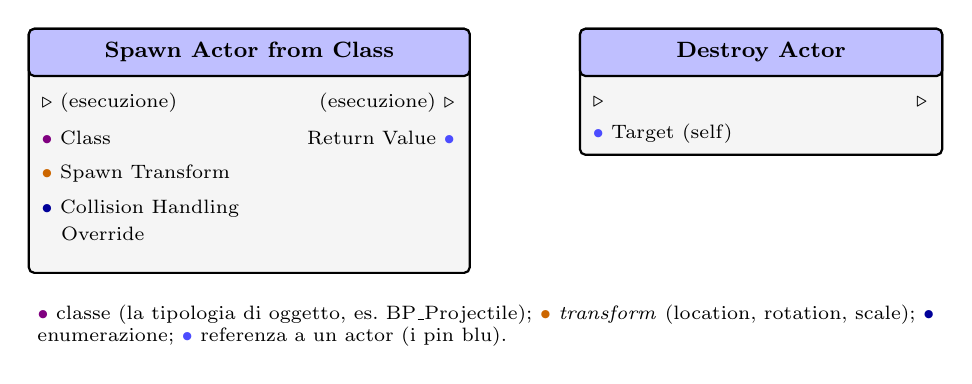
\begin{tikzpicture}[font=\footnotesize,
  ue5hdr/.style={draw, thick, fill=blue!25, minimum width=4.6cm, minimum height=0.6cm,
                 font=\footnotesize\bfseries, rounded corners=2pt},
  ue5bodyb/.style={draw, thick, fill=gray!8, minimum width=4.6cm, rounded corners=2pt},
  ue5pin/.style={font=\scriptsize, anchor=west},
  ue5pino/.style={font=\scriptsize, anchor=east}]
  % --- Spawn Actor from Class
  \node[ue5bodyb, minimum height=3.1cm, minimum width=5.6cm, anchor=north west] (sb)
    at (0,0) {};
  \node[ue5hdr, minimum width=5.6cm, anchor=north west] at (0,0) {Spawn Actor from
    Class};
  \node[ue5pin] at (0.05,-0.95) {$\triangleright$ (esecuzione)};
  \node[ue5pin] at (0.05,-1.4) {\textcolor{violet}{$\bullet$} Class};
  \node[ue5pin] at (0.05,-1.85) {\textcolor{orange!80!black}{$\bullet$} Spawn Transform};
  \node[ue5pin] at (0.05,-2.3) {\textcolor{blue!60!black}{$\bullet$} Collision Handling};
  \node[ue5pin] at (0.3,-2.62) {Override};
  \node[ue5pino] at (5.55,-0.95) {(esecuzione) $\triangleright$};
  \node[ue5pino] at (5.55,-1.4) {Return Value \textcolor{blue!70}{$\bullet$}};
  % --- Destroy Actor
  \node[ue5bodyb, minimum height=1.6cm, anchor=north west] at (7.0,0) {};
  \node[ue5hdr, anchor=north west] at (7.0,0) {Destroy Actor};
  \node[ue5pin] at (7.05,-0.95) {$\triangleright$};
  \node[ue5pin] at (7.05,-1.35) {\textcolor{blue!70}{$\bullet$} Target (self)};
  \node[ue5pino] at (11.55,-0.95) {$\triangleright$};
  % --- legenda
  \node[align=left, font=\scriptsize, anchor=north west, text width=11.4cm] at (0,-3.4)
    {\textcolor{violet}{$\bullet$} classe (la tipologia di oggetto, es.\ BP\_Projectile);
     \textcolor{orange!80!black}{$\bullet$} \emph{transform} (location, rotation,
     scale); \textcolor{blue!60!black}{$\bullet$} enumerazione;
     \textcolor{blue!70}{$\bullet$} referenza a un actor (i pin blu).};
\end{tikzpicture}
\caption{I due nodi della slide sullo spawn: in ingresso la classe da creare, il
\emph{transform} e il modo di gestire le collisioni; in uscita, la referenza all'actor
appena creato. Destroy Actor prende solo l'actor da distruggere. I colori dei pin
seguono le convenzioni dell'editor. Schema ricostruito.}
\label{ue5:fig:spawnnodes}
\end{figure}

\paragraph{Approfondimento: Collision Handling Override.} Il menù a tendina decide che
cosa fare se, nel punto di spawn, l'actor si troverebbe compenetrato con qualcos'altro.
Le opzioni sono: \emph{Default} (usa l'impostazione della classe), \emph{Always Spawn,
Ignore Collisions} (spawna comunque, anche dentro un muro), \emph{Try To Adjust
Location, But Always Spawn} (prova a spostarlo un poco, altrimenti spawna lì),
\emph{Try To Adjust Location, Don't Spawn If Still Colliding} (prova a spostarlo, e se
non trova posto non lo crea) e \emph{Do Not Spawn} (se c'è collisione, niente spawn).
Romero e Sewell (capitolo 3) suggeriscono anche di \textbf{promuovere a variabile} il
Return Value (tasto destro, \emph{Promote to Variable}) se l'oggetto creato servirà più
tardi, per esempio per distruggerlo; prima di usarla, la variabile va controllata con
un \textbf{Is Valid}, perché l'actor potrebbe essere già stato distrutto.

% ---------------------------------------------------------------------
\section{I cicli e il For Loop}
\label{ue5:sec:cicli}

``Anche un'altra cosa che andremo a vedere oggi sarà il \textbf{for loop}. Qualcuno ha
mai sentito parlare di \textbf{cicli} in programmazione?'' Uno studente che ha studiato
il C (``conosco \emph{while}, \emph{do while}, \emph{for}'') dà la definizione: ``è
ripetere un insieme di linee di codice finché una condizione è soddisfatta''. E fa un
esempio sulla torretta: ``finché il player sta in range della torretta, la torretta si
deve muovere; appena esce, quel codice non deve essere più ripetuto''. ``Sì,
assolutamente.''

Oggi, spiega il docente, si costruirà un actor che spawna dei cubetti ``in linea e in
colonne'': ``fondamentalmente andiamo a fare una \textbf{matrice}'', ``come in Excel,
ragazzi: le matrici per righe e colonne''. E lo si farà ``non uno per uno, ma tramite un
\textbf{indice}'': il For Loop è ``un modo iterativo di eseguire il codice fino a che
l'indice, quindi un numero che fa da dire OK, fatto il primo, OK, fatto il secondo, OK,
fatto il terzo\ldots{} Se arrivi a 10, smetti''. I cicli, infine, ``possono essere
innestati: cicli dentro altri cicli'', ed è esattamente ciò che servirà per righe e
colonne.

\paragraph{Approfondimento: i cicli dei Blueprint.} Nei Blueprint i cicli sono nodi di
\emph{flow control}. \textbf{For Loop} ha due ingressi interi, \textbf{First Index} e
\textbf{Last Index}, ed esegue il pin \textbf{Loop Body} una volta per ogni valore
dell'indice, dal primo all'ultimo \emph{compresi}, esponendo il valore corrente sul pin
\textbf{Index}; alla fine esegue \textbf{Completed}. \textbf{For Each Loop} fa lo stesso
scorrendo gli elementi di un array (Romero e Sewell, capitolo 13, lo usano per accendere
tutte le luci di una stanza). \textbf{While Loop} ripete finché una condizione booleana
è vera, come il \emph{while} del C. Una cosa importante, che distingue i cicli dei
Blueprint dal tempo del gioco: un For Loop si esegue \textbf{tutto nello stesso
\emph{frame}}, non ``piano piano nel tempo''. Non può contenere un Delay, e un ciclo
troppo lungo (o un While che non finisce mai) blocca il gioco; Unreal lo interrompe con
un errore di \emph{infinite loop} dopo un numero massimo di iterazioni. Per ripetere
qualcosa nel tempo si usano il Tick o i timer, come la torretta della quarta lezione.

% ---------------------------------------------------------------------
\section{Il fix della torretta: Find Relative Look at Rotation}
\label{ue5:sec:relative}

Prima dei proiettili, ``andremo a fissare una piccola cosa''. Il problema è quello visto
la volta scorsa: la torretta è fatta di tre \emph{static mesh}, e a ruotare è un solo
\emph{componente}, il Pivot, che ruota \textbf{rispetto al suo genitore}, la base. Find
Look at Rotation, invece, ``prenderà la rotazione in confronto a quella del
\textbf{mondo}, cioè di come è posizionato nel mondo''. Finché la torretta non è ruotata
nel livello le due cose coincidono; ma ``io giro la torretta a 90 gradi in engine, e poi
mi fa un offset di 90''.

\paragraph{La scoperta.} ``Ho scoperto, ed è una bellissima cosa, oserei dire, che Unreal
ci mette a disposizione il \textbf{Find Relative Look at Rotation} direttamente.'' Il
nodo ``prende il suo \emph{transform} e ci fa a quel punto un Find Look at Rotation in
relativa''. In pratica, in MoveTurret (il Custom Event chiamato dal timer):
\begin{itemize}
  \item si fa apparire \textbf{Find Relative Look at Rotation} al posto di Find Look at
        Rotation;
  \item al \textbf{Target} si collega quello che c'era già: la posizione del
        bersaglio, Get Actor Location di PlayerTarget;
  \item allo \textbf{Start Transform}, che chiede ``da che \emph{transform}
        partiamo'', si collega \textbf{Get Actor Transform} della torretta;
  \item l'uscita resta splittata, con la sola \textbf{Z} (lo \emph{yaw}) collegata al
        Target di \textbf{RInterp To}: ``questo non cambia assolutamente nulla''.
\end{itemize}
``Facendo ciò, da quel punto in poi la nostra torretta la possiamo ruotare come ci pare.
Tanto lui prenderà sempre a livello relativo.'' Il docente gira la torretta nel livello,
entra nel raggio: ``ecco che ci segue, senza cambiamenti, senza niente''
(figura~\ref{ue5:fig:relative}).

\paragraph{La velocità di interpolazione.} Il docente aveva trasformato l'Interp Speed in
una variabile e ``vi dico già che 0,01 era molto basso. Con questo find relative, ho
messo \textbf{2} e mi va più che bene. È anche più corretto''. A uno studente che non
sapeva come fosse nata la variabile: ``tira fuori dal pin, c'è scritto \emph{Promote to
Variable}''; poi si compila e, in basso a destra, nel \emph{Default Value}, si mette 2.
E, ``intanto'', il \textbf{Delta Time}: ``tira fuori dal Delta Time un pin e fai
\textbf{Get World Delta Seconds}''.

\begin{figure}[htbp]
\centering
\begin{tikzpicture}[font=\footnotesize,
  ue5node/.style={draw, thick, rounded corners=4pt, align=center, fill=gray!8,
                  minimum height=0.85cm, text width=2.4cm},
  ue5event/.style={ue5node, fill=red!12},
  ue5exec/.style={-{Stealth[length=2.5mm]}, very thick, black!80},
  ue5data/.style={-{Stealth[length=2mm]}, thick, blue!60!black},
  ue5trf/.style={-{Stealth[length=2mm]}, thick, orange!80!black},
  ue5flt/.style={-{Stealth[length=2mm]}, thick, green!50!black}]
  \node[ue5event] (mv) at (0,0) {\textbf{Custom Event}\\\textbf{MoveTurret}};
  \node[ue5node] (iv) at (3.1,0) {\textbf{Is Valid}\\PlayerTarget};
  \node[ue5node, text width=2.9cm] (srr) at (11.0,0) {\textbf{Set Relative
    Rotation}\\Target: Pivot};
  \draw[ue5exec] (mv) -- (iv);
  \draw[ue5exec] (iv) -- node[above, font=\scriptsize]{Is Valid} (srr);
  % dati
  \node[ue5node, fill=orange!12] (gat) at (0,-2.2) {\textbf{Get Actor
    Transform}\\(self)};
  \node[ue5node] (gal) at (0,-3.6) {\textbf{Get Actor Location}\\di PlayerTarget};
  \node[ue5node, text width=3.0cm, fill=yellow!20] (frl) at (3.6,-2.9)
    {\textbf{Find Relative Look at Rotation}\\Start Transform\\Target};
  \node[ue5node, text width=2.8cm] (ri) at (7.4,-2.9) {\textbf{RInterp To}\\
    Current: Get Relative Rotation (Pivot)\\Target: solo Z};
  \node[ue5node] (gwd) at (7.4,-5.0) {\textbf{Get World Delta Seconds}};
  \node[ue5node] (spd) at (4.1,-5.0) {\textbf{InterpSpeed}\\(variabile, 2)};
  \draw[ue5trf] (gat) -- (frl);
  \draw[ue5data] (gal) -- (frl);
  \draw[ue5flt] (frl) -- node[above, font=\scriptsize]{Z} (ri);
  \draw[ue5flt] (gwd) -- node[right, font=\scriptsize]{Delta Time} (ri);
  \draw[ue5flt] (spd) -- node[below, font=\scriptsize, pos=0.7]{Interp Speed} (ri);
  \draw[ue5flt] (ri.east) -| (srr.south);
\end{tikzpicture}
\caption{MoveTurret dopo il \emph{fix}. Il nodo nuovo (in giallo) calcola la rotazione
verso il bersaglio nello spazio della torretta, a partire dal suo \emph{transform}:
la torretta si può girare nel livello senza offset. Delta Time viene ora da Get World
Delta Seconds e l'Interp Speed, promosso a variabile, vale 2. Schema ricostruito.}
\label{ue5:fig:relative}
\end{figure}

\paragraph{Lo studente con la torretta che non gira.} Il primo caso in condivisione è
quello di uno studente che ha perso le lezioni precedenti per un problema al computer.
Il pivot non era stato reimportato a $-113$ (``non me l'ha fatto fare'', il re-import
non partiva). Lo si reimporta trascinando il file del materiale didattico nel
\emph{Content Browser} (attenzione a non lasciarlo cadere sopra altre cartelle); poi, in
scena, il pivot è ``storto'': lo si raddrizza con la modalità \textbf{Modeling}
(\textbf{Shift+5}), strumento \textbf{XForm}, \emph{Edit Pivot}. Nel Blueprint il pivot è
``un po' interrato'', e il cannone va staccato e riattaccato. Alla fine ruota, ``c'è un
piccolo offset, ma è importante che ruoti'', e punta ``dall'altra parte'': il caso è
rimandato alla pausa (sezione~\ref{ue5:sec:pausa}).

\paragraph{Approfondimento: perché il nodo nuovo risolve.} Find Relative Look at
Rotation (\emph{Start Transform}, \emph{Target Location}) trasforma prima il punto
bersaglio nello spazio locale del \emph{transform} di partenza, e poi calcola la
rotazione per guardarlo da lì. Il risultato è quindi già una rotazione
\textbf{relativa} all'actor, la stessa grandezza che Set Relative Rotation imposta sul
Pivot: i due spazi, che nel grafo della quarta lezione erano mescolati, ora coincidono.
Restano due avvertenze. Il punto di partenza è l'origine dell'actor, la base: va bene
per lo \emph{yaw}, ma per un \emph{pitch} preciso converrebbe partire dal
\emph{transform} del Pivot o del cannone (Get World Transform sul componente). E l'offset
dovuto alla \emph{mesh} reimportata a 113 gradi resta: il nodo presuppone che la
torretta, a rotazione zero, guardi lungo la propria X. Quanto alla velocità: con Delta
Time preso da Get World Delta Seconds e Interp Speed 2, il prodotto è circa 0,02 a 100
\emph{frame} al secondo, e la torretta insegue in modo morbido e uguale su ogni
macchina, come anticipato nella lezione precedente.

% ---------------------------------------------------------------------
\section{I trace: linee immaginarie}
\label{ue5:sec:trace}

``Abbiamo parlato di spawn, ma anche una cosa che andremo a vedere è chiamata
\textbf{line trace}.'' ``Oggi usiamo lo \textbf{sphere trace}, però in generale un trace
è una \textbf{linea immaginaria} che viene fatta dall'engine'' per scoprire che cosa c'è
lungo un percorso.

\paragraph{La dimostrazione.} Il docente lo mostra con la torretta che aveva già
preparato (``ecco qua, spawnano la marea di proiettili''). Entrando nel raggio, davanti
al cannone compare un \textbf{reticolo rosso}: ``una linea immaginaria, che non vedremo
se dovessimo avere un eseguibile''. Ma ``vedete che è rosso, rosso, rosso; se
\emph{overlappa}, diventa \textbf{verde}. Dice: ah, ho visto qualcosa! E quindi comincia
a sparare''. Poi, per confronto, trasforma al volo lo sphere trace in un \textbf{Line
Trace by Channel}: ``facciamo una linea''. All'inizio la linea non trova nulla, ``perché
è impostata male''; basta cambiarle il canale, e ``ecco che ci ha trovato'': ``fa rosso
il puntino e verde. Dice: ah, ok, ti ho beccato''.

\paragraph{A che cosa servono.} ``Sono delle linee immaginarie che servono a noi
\emph{developer} per dire: oh, c'è qualcosa che overlappa una linea invisibile?
Effettivamente sì, effettivamente no.'' Il docente racconta di averle usate per
un'intelligenza artificiale: ``tracciavo una linea tra me e il player; se c'era qualcosa
di mezzo, vuol dire che non lo vedeva; se invece non c'era niente, vuol dire che lo
vedeva''. È ``proprio una \textbf{linea di vista}''. E un avvertimento, ripetuto:
``non esagerate con il trace, perché anche esso è molto pesante'', tanto più se, come
oggi, lo si fa a ogni \emph{frame}.

\paragraph{Approfondimento: le famiglie di trace.} Romero e Sewell (capitolo 14)
definiscono i trace come test di collisione lungo un segmento. Ne esistono di due
tipi di ``filtro'': \textbf{by Channel}, che cercano gli oggetti che bloccano un
\emph{trace channel} (Visibility, Camera o un canale creato da noi), e \textbf{for
Objects}, che cercano gli oggetti di certi \emph{object type} (WorldStatic,
WorldDynamic, Pawn, PhysicsBody, Vehicle, Destructible). E di quattro forme: la
\textbf{linea}, la \textbf{sfera}, la \textbf{capsula} e il \textbf{box}, dove le forme
``spesse'' sono più costose della linea. Infine, ogni trace ha una versione singola,
che restituisce il primo oggetto colpito, e una \textbf{Multi}, che li restituisce
tutti (sezione~\ref{ue5:sec:errori}). Tutti hanno gli stessi ingressi principali:
\textbf{Start} ed \textbf{End}, il canale o i tipi, \textbf{Trace Complex} (testare
contro la \emph{mesh} vera o contro le forme di collisione semplificate), \textbf{Actors
to Ignore}, \textbf{Draw Debug Type} e \textbf{Ignore Self}. Le uscite sono un
\textbf{Out Hit} (una struttura \emph{Hit Result} con, tra l'altro, il punto d'impatto,
la normale della superficie e l'actor colpito, leggibili con \emph{Break Hit Result}) e
un \textbf{Return Value} booleano: vero se qualcosa ha bloccato il trace.

% ---------------------------------------------------------------------
\section{L'evento Shoot e i vettori del trace}
\label{ue5:sec:shoot}

``La prima cosa è che dobbiamo creare un evento \textbf{Shoot}'': un \textbf{Custom
Event} nel grafo di BP\_Turret.

\paragraph{Is Valid, per buona maniera.} ``Intanto la prima cosa che andiamo a fare è
vedere se esiste il target'': un \textbf{Is Valid} (``la macro con il punto
interrogativo'') su PlayerTarget. ``È buona maniera fare questa cosa, di vedere se
effettivamente esiste o non esiste, perché ci ottimizza i processi'': se non c'è un
bersaglio, non si esegue nulla. (Più avanti, nella sezione~\ref{ue5:sec:bocche}, questo
Is Valid verrà spostato fuori da Shoot.)

\paragraph{Lo Sphere Trace by Channel.} Poi lo \textbf{Sphere Trace by Channel}: ``una
linea immaginaria che andremo a creare in modo tale che, se il nostro character entra in
questa sfera, vuol dire che io lo sto vedendo ed è in puntamento''. Che cosa chiede?
``Un punto di \textbf{Start} e un punto di \textbf{End}'', con i pin
\textbf{gialli}. ``Chi si ricorda quali sono gli elementi gialli in Unreal?'' ``Un
vettore.'' ``Bravissimo, è un vettore. In questo caso, un vettore di locazione'': una X,
una Y e una Z.

\paragraph{Il punto di partenza: TraceSpawn.} Il trace deve partire ``più o meno dalla
canna, da questo punto qua in avanti''. Si potrebbe usare la posizione del Pivot, ``però
vi dico che è più corretto fare una cosa del genere: andiamo a creare proprio un
\textbf{punto vuoto}'' dedicato. Nei componenti si fa \emph{Add} e si scrive
\textbf{Scene}: un \emph{Scene Component}, ``solo un punto nello spazio'', senza
\emph{mesh} né collisioni. Lo si \textbf{attacca al cannone}, lo si posiziona ``in
mezzo alle due canne'', e lo si rinomina (``per rinominare le cose molto più
velocemente: cliccate sull'elemento, \textbf{F2}, e scrivete'') in
\textbf{TraceSpawn}. ``L'abbiamo attaccato al cannone perché il pivot fa ruotare il
cannone e il cannone farà ruotare il TraceSpawn: c'è questa \textbf{dipendenza a
cascata}.'' Dal componente TraceSpawn si prende \textbf{Get World Location}, ``dove è
posizionato nel mondo'', e la si collega allo \textbf{Start}.

\paragraph{Il punto d'arrivo: il forward vector.} ``Ci manca quello del punto di fine.
Dove deve arrivare?'' Qui torna la teoria dei vettori della quarta lezione. Ogni
\emph{mesh}, ogni componente, ogni actor ha dei vettori di direzione ``già prefatti'':
\begin{itemize}
  \item \textbf{Get Actor Forward Vector}, che ``punterà sempre in avanti'';
  \item \textbf{Get Actor Right Vector}, ``che punterà sempre a destra'';
  \item \textbf{Get Actor Up Vector}, ``che punterà sempre in alto'',
\end{itemize}
sempre relativi all'oggetto. ``Domanda: se io moltiplicassi per $-1$ il forward vector,
dove punterà rispetto alla mesh?'' ``Dietro.'' ``Bravissimo'': moltiplicare per $-1$
``inverte il risultato''; così si ottengono il \emph{back} vector, la sinistra e il
basso.

\paragraph{Lungo 1: moltiplicare.} Ma se si collega il forward vector così com'è ``non ci
darà assolutamente nulla, perché è molto piccolo'': ``il forward vector che ci dà Unreal
è di \textbf{lunghezza 1}'', un vettore normalizzato. ``Buona prassi è prenderlo e
moltiplicarlo, per esempio per \textbf{800}'': ``avremo un vettore 800 volte più
lungo''. (Uno studente non riesce a scrivere 800 nel Multiply: ``il pallino è giallo e
non verde''. ``Se moltiplicate un vettore, vi dà direttamente la moltiplicazione per un
altro vettore, ma potete cambiare il secondo fattore: tasto destro, \emph{To Float}.
Diventerà verde, e ci mettete 800.'')

\paragraph{Un punto non è una linea: sommare.} ``Magari vi verrebbe da dire: ok, ho
trovato il punto laggiù, lo vado a mettere nell'End. No, ancora no.'' Il forward vector
moltiplicato è ``un punto, non è una linea'': è uno spostamento di 800 in avanti,
calcolato come se si partisse dall'origine del mondo. ``Per farlo diventare una linea
dobbiamo letteralmente \textbf{sommare} due vettori'': la World Location di TraceSpawn
più il forward vector per 800. ``È un discorso che sembra strano, però effettivamente
quello che abbiamo qua è solo un punto nello spazio; con la somma ne traiamo un'effettiva
linea'' (figura~\ref{ue5:fig:vettori}).

\paragraph{Il forward vector giusto.} Alla prima prova il trace c'è, ma ``non segue il
pivot'': resta fermo mentre la torretta ruota. Il motivo: Get \emph{Actor} Forward
Vector è il vettore dell'actor intero, cioè della \textbf{base}, ``quindi sarà sempre lì.
Non girerà, perché deve girare insieme al cannone''. La correzione: ``invece di prendere
il Get Actor Forward Vector, prendiamo il \textbf{Get Forward Vector del TraceSpawn}''.
(``A me non fa collegare TraceSpawn e Get Forward Vector'': bisogna tirare il filo
\emph{dal} componente TraceSpawn e cercare \emph{Get Forward Vector}, la versione per i
componenti.)

\begin{figure}[htbp]
\centering
\begin{tikzpicture}[font=\footnotesize, >={Stealth[length=2.5mm]}]
  % assi del mondo
  \draw[->, thick, gray] (-0.3,0) -- (2.0,0) node[right]{X};
  \draw[->, thick, gray] (0,-0.3) -- (0,1.8) node[above]{Y};
  \node[below left, gray, font=\scriptsize] at (0,0) {origine del mondo};
  % torretta vista dall'alto
  \coordinate (C) at (6.0,0.4);
  \fill[gray!25, draw=black, thick] (C) circle (0.7);
  \node[font=\scriptsize, below] at ($(C)+(0,-0.7)$) {base};
  \begin{scope}[rotate around={35:(C)}]
    \fill[orange!25, draw=black, thick] ($(C)+(0,-0.2)$) rectangle ($(C)+(1.3,0.2)$);
  \end{scope}
  \coordinate (S) at ($(C)+(35:1.15)$);
  \fill[blue!60] (S) circle (0.07);
  \node[font=\scriptsize, align=center] at ($(S)+(-0.9,0.55)$) {TraceSpawn\\(Start)};
  % vettore posizione
  \draw[->, very thick, blue!60!black] (0,0) -- (S) node[pos=0.45, below, sloped,
    font=\scriptsize] {Get World Location};
  % forward unitario all'origine
  \draw[->, very thick, red!70!black] (0,0) -- (35:0.8);
  % forward x 800 all'origine (punto sbagliato)
  \draw[->, thick, red!70!black, dashed] (0,0) -- (35:3.6);
  \fill[red!70!black] (35:3.6) circle (0.06);
  \node[red!70!black, font=\scriptsize, align=left, anchor=south east] at (35:3.6)
    {Forward $\times$ 800\\(da solo: un punto\\vicino all'origine)};
  \node[red!70!black, font=\scriptsize, anchor=north west] at (0.15,-0.25)
    {Forward: lunghezza 1};
  % fine = start + forward x 800
  \coordinate (E) at ($(S)+(35:3.6)$);
  \draw[->, very thick, green!45!black] (S) -- (E);
  \fill[green!45!black] (E) circle (0.07);
  \node[right=3pt, green!45!black, align=left] at (E) {End =\\Start + Forward
    $\times$ 800};
  % sfera del trace
  \foreach \t in {0.2,0.45,0.7,0.95} {
    \draw[green!45!black, thin] ($(S)!\t!(E)$) circle (0.32);
  }
  \node[green!45!black, font=\scriptsize, anchor=west] at ($(S)!0.5!(E)+(0.45,-0.3)$)
    {Sphere Trace, Radius 80};
\end{tikzpicture}
\caption{I vettori del trace, visti dall'alto. Get World Location di TraceSpawn è un
vettore dall'origine del mondo al punto di partenza. Il Forward Vector è lungo 1;
moltiplicato per 800 diventa uno spostamento, che però, preso da solo, indica un punto
vicino all'origine (tratteggio). Sommato alla posizione di partenza, dà la fine giusta:
800 unità davanti alla canna. Lo sphere trace ``trascina'' una sfera di raggio 80 lungo
il segmento. Schema ricostruito, non in scala.}
\label{ue5:fig:vettori}
\end{figure}

\paragraph{Il raggio e il debug.} Due dettagli ancora. Il \textbf{Radius} dello sphere
trace parte da zero: ``il raggio della nostra bellissima sfera sarà zero, quindi non
esisterà''. Il docente mette \textbf{80}. E per vedere il trace in editor, ``lo vedremo
solo noi \emph{developer}'', c'è \textbf{Draw Debug Type}, da impostare su \textbf{For
One Frame}: ``perché se adesso la mettiamo \emph{For Duration}, ha una durata, sarà un
casino, perché lo fa ogni \emph{frame}'' (tabella~\ref{ue5:tab:debug}). Per provarlo,
Shoot viene chiamato dall'\textbf{Event Tick} (``prendete il Tick, scrivete Shoot,
come avete chiamato questo evento''): ``giusto per vedere effettivamente che
funzioni''.

\begin{table}[htbp]
\centering
\small
\begin{tabular}{@{}p{3.0cm}p{11.0cm}@{}}
\toprule
\textbf{Draw Debug Type} & \textbf{Che cosa disegna} \\
\midrule
None & niente: il trace c'è, ma non si vede (il valore di default) \\
For One Frame & il trace per un solo \emph{frame}: se il trace è chiamato a ogni
\emph{frame}, si vede ``in diretta''; è l'opzione usata a lezione \\
For Duration & il trace resta visibile per un certo tempo (Draw Time, nei dettagli del
nodo): chiamato a ogni \emph{frame}, accumula centinaia di disegni sovrapposti \\
Persistent & il trace resta disegnato per sempre: utile per un trace singolo, da
esaminare con calma \\
\bottomrule
\end{tabular}
\caption{Le opzioni di Draw Debug Type dei nodi di trace. I colori del disegno sono il
rosso per il tratto libero e il verde dal punto in cui il trace è stato bloccato (Trace
Color e Trace Hit Color, modificabili nel nodo).}
\label{ue5:tab:debug}
\end{table}

\paragraph{I problemi del momento.} Le condivisioni mostrano errori ricorrenti: lo
Start e l'End scambiati o collegati senza la somma (``Start è questo, solo questo; lo
attacchi così; il più va nell'End''); Draw Debug Type lasciato su \emph{None}; Shoot non
chiamato dal Tick (``l'hai messo sul Tick? Ah, no. Metti l'evento Shoot sul Tick''); e
la linea che compare ma non ruota con il cannone, per il motivo visto sopra.

% ---------------------------------------------------------------------
\section{I trace channel e le risposte di collisione}
\label{ue5:sec:canali}

Ora il trace c'è e ruota, ``ma come potete vedere non abbiamo il verdino, non ci dice
\emph{ho trovato}'': il player ci passa attraverso senza essere visto. Il motivo è il
\textbf{trace channel}. ``Di standard Unreal ci dà due canali, che sono
\textbf{Visibility} e \textbf{Camera}''; quello del docente (``questo qua al testo lo
vedete, l'ho creato io'') è un canale \textbf{custom}, che risponde ``in una certa
maniera, dipendentemente da certe opzioni''. Bisogna crearlo.

\paragraph{Creare il canale.} Dal menù \textbf{Edit}, \textbf{Project Settings}; si scende
``giù giù giù giù'' fino a \textbf{Collision} (nella sezione \emph{Engine}). Lì,
\textbf{New Trace Channel}: ``lo chiamate come volete, lo chiamiamo magari
\textbf{DetectionTurret}'', con \textbf{Default Response} su \textbf{Ignore}. Che cosa
vuol dire? ``Guarda questo trace: in risposta a tutti gli altri elementi in cui può
collidere, cosa fa di base? Ignora tutto, perché è meglio che ignori tutto, in modo tale
che tanto deve trovare solo il player.'' Se si mettesse \emph{Block}, ``ci bloccherebbe
tutto quanto'', e bisognerebbe togliere il blocco a tutti gli elementi statici e
dinamici. ``È più facile mettere ignora tutto, e poi mettiamo il \emph{tick} positivo al
nostro player.''

\paragraph{Il player risponde Block.} Si apre il \textbf{Third Person Character}, si
seleziona la \textbf{Mesh} e si cerca \emph{Collision} nei dettagli (``importante che, se
non avete compilato, compilate, perché se no non vi apparirà mai il nostro
DetectionTurret''). I \textbf{Collision Presets} sono grigi, perché è attivo un
\emph{preset}: si sceglie \textbf{Custom} dalla tendina, e nella riga di DetectionTurret
si mette la spunta su \textbf{Block}. ``In che modo reagisci al trace channel della
nostra torretta? Overlap, Block, Ignore. In questo caso andiamo a fare che blocca.''

\paragraph{Ignore, Overlap, Block.} Il docente ripassa le tre risposte con le mani:
``questa è la mia mano, l'oggetto 1, l'oggetto 2''. Con l'\textbf{Overlap}, ``se si
toccano non c'è una collisione fisica, quindi volendo si trapassano'', ma ``c'è una
\emph{detection}: l'engine dice, sono loro che collidono, quindi c'è un segnale''; è ciò
che si usa ``per i blocchi invisibili''. Il \textbf{Block}, invece, ``è proprio un
blocco fisico''. Il trace non ha un corpo, quindi per lui il Block è ``semplicemente
un'accortezza'': ``ehi, ho trovato il player, mi blocco''; ed è grazie al blocco che
appare la sfera ``parte verde, parte rossa'' (tabella~\ref{ue5:tab:risposte}).

\begin{table}[htbp]
\centering
\small
\begin{tabular}{@{}p{2.0cm}p{5.6cm}p{6.4cm}@{}}
\toprule
\textbf{Risposta} & \textbf{Tra due corpi} & \textbf{Per un trace} \\
\midrule
Ignore & si attraversano e nessuno se ne accorge & l'oggetto è invisibile per quel
trace \\
Overlap & si attraversano, ma scatta un evento di \emph{overlap} (i ``blocchi
invisibili'', la sfera della torretta) & il trace lo registra ma prosegue: lo vede solo
un trace Multi, e il Return Value resta falso \\
Block & si fermano l'uno contro l'altro: collisione fisica & il trace si ferma lì: è un
\emph{hit}, il disegno di debug diventa verde e il Return Value è vero \\
\bottomrule
\end{tabular}
\caption{Le tre risposte di collisione. Ogni componente dichiara una risposta per ogni
canale (Visibility, Camera, i canali custom) e per ogni \emph{object type}; quando due
oggetti si incontrano, vale la risposta più ``debole'' delle due.}
\label{ue5:tab:risposte}
\end{table}

\paragraph{Scegliere il canale nel trace.} Tornati in BP\_Turret, nello Sphere Trace by
Channel di Shoot si apre la tendina \textbf{Trace Channel}: ``c'è Visibility, Camera e
DetectionTurret''. Se compaiono solo Visibility e Camera, ``vai con \textbf{Compile},
qui in alto a sinistra''. In Play: ``vedete che è diventato verde. C'è il trace rosso,
viene bloccato, e da lì in poi c'è quello spazio verde'': ``è da lì in poi che il nostro
player è presente''. Avvicinandosi, il tratto verde si allunga.

\paragraph{Il Return Value.} Infine un \textbf{Print String} collegato al
\textbf{Return Value} del trace, ``che ci dice letteralmente: hai preso qualcosa? Sì,
no''. È un \textbf{booleano}: falso se non ha trovato niente, vero se ha trovato
qualcosa. In Play ``spunteranno un botto di true e false, ma è normale, sta sul Tick'':
``false, false, false\ldots{} true, true, true''.

\paragraph{Approfondimento: Mesh o Capsule?} A lezione la risposta Block al canale
DetectionTurret viene data alla \textbf{Mesh} del personaggio, e funziona. Nel Third
Person Character, però, il componente che rappresenta il corpo ai fini delle collisioni
è la \textbf{Capsule Component}, la radice; la Mesh scheletrica, di default, usa un
\emph{preset} (\emph{CharacterMesh}) pensato per non interferire con il movimento. Dare
il Block alla Mesh significa che il trace colpisce la forma del personaggio, con le sue
parti fisiche; darlo alla capsula significa colpire un cilindro più semplice. Entrambe
le scelte sono legittime; l'importante è sapere quale si è fatta, perché l'\emph{Hit
Actor} sarà lo stesso, ma l'\emph{Hit Component} e il punto d'impatto no.

% ---------------------------------------------------------------------
\section{Il proiettile: BP\_Projectile e il Projectile Movement}
\label{ue5:sec:proiettile}

``Abbiamo fatto la torretta che gira, abbiamo fatto la torretta che detecta: adesso
dobbiamo far sparare.'' Un Custom Event \textbf{SpawnProjectile}, ``ma che succede,
ragazzi? Non abbiamo un proiettile''. Lo si crea: tasto destro nel Content Browser,
\textbf{Blueprint Class}, \textbf{Actor}, e lo si chiama \textbf{BP\_Projectile}.

\paragraph{Due actor, due compiti.} Perché un Blueprint a parte, e non tutto dentro la
torretta? ``Due actor, uno che fa un compito e uno che fa un altro, è il miglior modo
per gestire i comportamenti.'' ``Perché a un certo punto magari vi arriva un
\emph{designer} e vi dice: ragazzi, non voglio che spawni più i proiettili, voglio che
spawni \textbf{banane}. Eh, se l'avete fatto dentro la torretta dovete fare un casino.
Invece, cambiare semplicemente il proiettile è molto più facile.''

\paragraph{La mesh.} Il proiettile è ``formato da due cose''. La prima è una \textbf{Static
Mesh}, rinominata \textbf{MeshProjectile}: una \textbf{sfera} di default (``se volete,
potete scaricare un modello, così ci mettete un proiettile al posto della palla'').
La si scala a \textbf{0,5}, poi a \textbf{0,3} (``mi sembra un po' grandicello''),
con il \textbf{lucchetto} della scala chiuso. ``Questo lucchetto l'abbiamo spiegato alla
prima lezione'': aperto, permette di modificare gli assi uno per uno; chiuso, ``se
modificate un singolo asse, vi scalerà anche le altre, in modo tale che rimangano
uniformi, perché sennò vengono forme stiracchiate''. Come materiale, \textbf{MI\_Solid\_Blue}
(``mi solid blue'').

\paragraph{Il Projectile Movement.} La seconda cosa è il movimento. ``Unreal ci arriva
con un regalo incredibile'': come la volta scorsa c'era il Rotating Movement per il
mulino, ``arriva la possibilità di avere un \textbf{Projectile Movement}, per quanti
giochi ormai hanno dei proiettili''. Si aggiunge il componente, e nei dettagli ci sono
``un sacco di dati in cui possiamo giocare'': ``tanti giochi ai giorni d'oggi hanno cose
molto comuni. Quanti FPS ce ne sono? Anche le armi di \emph{Borderlands}, che sono tutte
strane, alla base si parla sempre di sparare''. I valori della lezione:
\begin{itemize}
  \item \textbf{Initial Speed} 1000 e \textbf{Max Speed} 1000 (per guardarlo meglio, a
        un certo punto l'Initial Speed scende a 100, ``la lumaca'', e poi torna a 1000,
        ``una velocità da proiettile'');
  \item \textbf{Projectile Gravity Scale} a \textbf{0}: ``questo proiettile al momento
        è afflitto dalla gravità''; ``noi vogliamo che vada dritto per dritto'';
  \item \textbf{Velocity} lasciata a $(1, 0, 0)$: ``la velocità è la direzione'',
        quindi ``è 1 sull'asse X'', e il proiettile ``andrà dritto così''.
\end{itemize}
E la mesh deve essere \textbf{Movable}, ``se no vi danno errore''. Messo in scena e
avviato il Play, ``il nostro bellissimo proiettilino se ne va per la sua'' strada:
attraversa tutto, ``overlapperà, e chissà chi lo vedrà più''. (A una studentessa la
pallina ``cade semplicemente'': aveva lasciato la gravità a 1.)

\paragraph{Approfondimento: i parametri del Projectile Movement.} Romero e Sewell
(capitolo 6) modificano il proiettile del modello \emph{First Person} con gli stessi
parametri. \textbf{Initial Speed} è la velocità con cui il proiettile parte; \textbf{Max
Speed} è il limite, che conta solo se qualcos'altro lo accelera (un razzo con il motore
acceso); per un proiettile d'arma ha senso che le due coincidano. \textbf{Velocity} è
una direzione nello spazio \emph{locale} del proiettile: se Initial Speed è maggiore di
zero, Unreal ne usa solo la direzione e la moltiplica per l'Initial Speed. Per questo
è importante che lo spawn dia al proiettile la rotazione giusta: la X locale del
proiettile deve guardare fuori dalla canna. \textbf{Projectile Gravity Scale} moltiplica
la gravità del mondo (0 nessuna, 0,1 ``proiettile leggero''). La sezione \textbf{Projectile
Bounces}, con \emph{Should Bounce}, decide se rimbalza sui muri; e \textbf{Rotation Follows
Velocity} lo fa girare nella direzione del moto, utile per frecce e razzi.

% ---------------------------------------------------------------------
\section{Il proiettile che si distrugge}
\label{ue5:sec:distruzione}

``Noi vorremmo che il nostro proiettile sia molto più realistico: trova un muro e
scompare.'' E non è solo estetica: ``immaginatevi che adesso spawneremo dei proiettili
che andranno nell'infinito e oltre''; l'engine ``dirà: guarda, esiste'', e ``non
libereremo mai la memoria''.

\paragraph{Un trace attorno al proiettile.} La soluzione riusa il trace: nell'\textbf{Event
Tick} di BP\_Projectile, uno \textbf{Sphere Trace by Channel} di raggio \textbf{30},
``una sfera intorno al nostro proiettile che ci dirà: guarda, hai colpito qualcosa?''.
Start ed End sono \textbf{lo stesso punto}, \textbf{Get Actor Location} del proiettile:
``vogliamo che l'inizio e la fine siano lo stesso punto''. Con Draw Debug Type su For
One Frame, ``intorno alla nostra pallina si è creato un trace''.

\paragraph{Branch e Destroy Actor.} Poi: ``molto semplicemente, Return Value è vero? Sì?
Allora distruggete''. Un \textbf{Branch} (``tenete premuto B e cliccate'') sul Return
Value, e sul ramo True un \textbf{Destroy Actor} (figura~\ref{ue5:fig:proiettile}). In
Play, alla ``velocità della lumaca'', il proiettile arriva al muro e sparisce: ``si è
distrutto, quindi abbiamo il comportamento di base''. Il Tick, nota il docente,
``inizierà solamente quando l'oggetto esiste'': ogni proiettile controlla sé stesso
finché vive.

\begin{figure}[htbp]
\centering
\begin{tikzpicture}[font=\footnotesize,
  ue5node/.style={draw, thick, rounded corners=4pt, align=center, fill=gray!8,
                  minimum height=0.85cm, text width=2.5cm},
  ue5event/.style={ue5node, fill=red!12},
  ue5exec/.style={-{Stealth[length=2.5mm]}, very thick, black!80},
  ue5vec/.style={-{Stealth[length=2mm]}, thick, yellow!50!black},
  ue5bool/.style={-{Stealth[length=2mm]}, thick, red!60!black},
  ue5comp/.style={draw, thick, rounded corners=3pt, minimum width=3.5cm,
                  minimum height=0.55cm, align=center, font=\scriptsize}]
  % componenti
  \node[font=\scriptsize\bfseries] at (0,1.0) {BP\_Projectile: componenti};
  \node[ue5comp, fill=gray!20] (r) at (0,0.4) {DefaultSceneRoot};
  \node[ue5comp, fill=blue!20] (m) at (0.6,-0.3) {MeshProjectile (sfera, 0,3)};
  \node[ue5comp, fill=green!15] (pm) at (0,-1.0) {ProjectileMovement};
  \draw[thick, gray!60!black] ([xshift=-1.5cm]r.south) |- (m.west);
  \node[font=\scriptsize, align=left, anchor=west] at (-1.45,-1.75)
    {Initial / Max Speed 1000\\Gravity Scale 0, Velocity (1,0,0)};
  % grafo
  \node[ue5event] (tick) at (4.4,0.2) {\textbf{Event Tick}};
  \node[ue5node, text width=3.0cm] (st) at (7.9,0.2) {\textbf{Sphere Trace by
    Channel}\\Radius 30\\Channel: ProjectileTrace\\Debug: For One Frame};
  \node[ue5node, text width=1.6cm] (br) at (11.3,0.2) {\textbf{Branch}};
  \node[ue5node, text width=1.9cm] (de) at (11.3,-1.9) {\textbf{Destroy Actor}\\(self)};
  \node[ue5node] (gal) at (4.4,-1.6) {\textbf{Get Actor Location}\\(self)};
  \draw[ue5exec] (tick) -- (st);
  \draw[ue5exec] (st) -- (br);
  \draw[ue5exec] (br) -- node[right, font=\scriptsize]{True} (de);
  \draw[ue5vec] (gal.east) -| node[pos=0.75, left, font=\scriptsize, align=right]
    {Start\\e End} (st.south);
  \draw[ue5bool] ([yshift=-0.4cm]st.east) -- node[above, font=\scriptsize, pos=0.4]
    {Return Value} ([yshift=-0.4cm]br.west);
\end{tikzpicture}
\caption{Il proiettile. A sinistra i componenti: una sfera scalata e il Projectile
Movement, che fa tutto il moto. A destra il grafo: a ogni \emph{frame}, una sfera di
raggio 30 attorno al proiettile (Start ed End coincidono); se qualcosa la blocca, il
proiettile si distrugge. Il canale, all'inizio Visibility e poi Camera, diventa alla
fine ProjectileTrace. Schema ricostruito.}
\label{ue5:fig:proiettile}
\end{figure}

\paragraph{Approfondimento: altri modi di distruggere un proiettile.} Il trace sul Tick
funziona ed è istruttivo, ma non è l'unico modo, né il più economico. Il Projectile
Movement ha un proprio evento, \textbf{On Projectile Stop}, che scatta quando il
proiettile si ferma contro qualcosa che lo blocca; e un componente di collisione (una
Sphere Collision come radice del proiettile, con il Projectile Movement che la muove)
genera \textbf{Event Hit} o \textbf{On Component Hit} all'impatto. Romero e Sewell
(capitolo 6) collegano proprio all'evento di \emph{hit} il Destroy Actor, ``così che il
proiettile venga sempre distrutto quando collide''. Infine, per i proiettili che non
colpiscono nulla, l'actor ha una proprietà \textbf{Initial Life Span} (nei \emph{Class
Defaults}): se maggiore di zero, l'actor si distrugge da solo dopo quei secondi. È una
rete di sicurezza contro i proiettili che vanno ``nell'infinito e oltre''.

% ---------------------------------------------------------------------
\section{Visibility, Camera e il canale ProjectileTrace}
\label{ue5:sec:projtrace}

Il proiettile si distrugge contro il muro, ``anche il player, volendo?'' No: ``mi metto
davanti, e infatti non ce lo prende''. Con il canale \textbf{Visibility} il personaggio
non viene visto; cambiando il canale in \textbf{Camera}, ``così ci prende pure il
player''.

\paragraph{Perché.} Il docente apre le collisioni del Third Person Character: c'è la
tabella delle \textbf{Collision Responses}, con Ignore, Overlap e Block, e sotto le
\textbf{Trace Responses}, ``cioè come rispondo a questo trace''. ``Come rispondo al trace
Visibility? Vedete che c'è la spunta su Ignore; invece il Camera viene bloccato.''
``Semplicemente è un concetto di collisioni.''

\paragraph{Un canale per il proiettile.} ``Lo facciamo, ragazzi, così almeno è buona
prassi'': un secondo canale, \textbf{ProjectileTrace}. Qui il ragionamento è opposto a
quello di DetectionTurret. Il docente prima pensa a Ignore e a mettere il Block sui
quattro muri uno per uno (``però è più pesante''), poi cambia idea: ``è molto meglio
farlo in \textbf{Block}, così facciamo un Block e leviamo semplicemente quelli che non ci
interessano''. La regola generale: ``quante cose ho che devono bloccare, e quante che
devono ignorare?''. Il proiettile ``sbatte praticamente con tutto'', quindi Default
Response \textbf{Block}, e si escludono le poche eccezioni (tabella~\ref{ue5:tab:canali}):
\begin{itemize}
  \item il \emph{character}: Block (``va benissimo'');
  \item la \textbf{Sphere} della torretta, il raggio d'azione: Custom, ProjectileTrace
        su \textbf{Ignore}, altrimenti il proiettile esploderebbe appena nato, dentro la
        sfera;
  \item anche \textbf{Pivot}, \textbf{Base} e \textbf{Cannon}: ``non vogliamo che
        rimbalzi contro la stessa torretta che l'ha sparato'', quindi Custom e Ignore
        a tutti e tre.
\end{itemize}
Nel trace del proiettile si sceglie ProjectileTrace (``sempre compilato, perché se no non
vi arriva''), e in Play il proiettile si distrugge sia sul player sia sul muro.

\begin{table}[htbp]
\centering
\small
\begin{tabular}{@{}p{2.8cm}p{2.1cm}p{9.1cm}@{}}
\toprule
\textbf{Canale} & \textbf{Default} & \textbf{Eccezioni impostate a lezione} \\
\midrule
DetectionTurret & Ignore & Mesh del Third Person Character: \textbf{Block}. Il trace
della torretta vede solo il giocatore. \\
ProjectileTrace & Block & Sphere, Pivot, Base e Cannon della torretta: \textbf{Ignore};
dopo la pausa anche la sfera del proiettile stesso. Character: Block. Il proiettile si
ferma su tutto tranne che sulla torretta che lo spara. \\
\bottomrule
\end{tabular}
\caption{I due \emph{trace channel} creati in Project Settings $\rightarrow$ Engine
$\rightarrow$ Collision. Il principio: se le cose da colpire sono poche, Default
Ignore e Block sulle eccezioni; se sono molte, Default Block e Ignore sulle eccezioni.}
\label{ue5:tab:canali}
\end{table}

\paragraph{``A me passa attraverso.''} Due studenti hanno il proiettile che attraversa
player e muri (``il player me lo sposta, e i muri li attraversa''). Si controllano il
canale (Block), il nodo (ProjectileTrace), le collisioni della Mesh: tutto giusto. Il
colpevole è il \textbf{Radius}: ``era zero, quindi era invisibile''. ``Attenzione,
ragazzi, perché il radius è la grandezza: se è zero, non esiste.'' (E il raggio del
trace della torretta? ``80.'') Un'altra studentessa non trova i Collision Presets della
Sphere della torretta: bisogna selezionare proprio il componente \emph{Sphere} nella
lista dei componenti, e la sezione Collision compare.

\paragraph{Approfondimento: Ignore Self e Actors to Ignore.} Tutti i nodi di trace hanno
la casella \textbf{Ignore Self}, attiva di default: il trace ignora tutti i componenti
dell'actor che lo esegue. Il trace del proiettile, quindi, non vede la propria sfera
anche senza toccarne le collisioni, e quello della torretta non vede la torretta. Per
escludere \emph{altri} actor, senza modificare le loro collisioni, c'è l'ingresso
\textbf{Actors to Ignore}, un array: per esempio, il proiettile potrebbe ricevere allo
spawn una referenza alla torretta che l'ha sparato (i pin \emph{Owner} e \emph{Instigator}, che compaiono espandendo
Spawn Actor from Class, servono proprio a passare questo genere di informazione) e ignorarla nel trace. È la soluzione più pulita quando le torrette sono tante e
ognuna deve ignorare solo i propri colpi.

% ---------------------------------------------------------------------
\section{La pausa e i problemi degli studenti}
\label{ue5:sec:pausa}

Il docente crea il Custom Event SpawnProjectile e tira fuori \textbf{Spawn Actor from
Class}; poi guarda l'ora: ``sono le 17 e 28. Vogliamo fare pausa adesso, per fare lo
spawn dopo?'' La classe vota per la pausa, ``i classici 20 minuti'', alle 17:50. Ma chi
ha problemi resta, e la pausa diventa un lungo giro di condivisioni, utile soprattutto
per le tecniche di \emph{debug} che mostra.

\paragraph{Le collisioni della torretta.} Il primo caso è rapido: come si toglie la
collisione con il proiettile a Gun, Pivot e Base? ``Devi cliccare su ogni asset,
Collision Presets, fai Custom, Ignore a ProjectileTrace. A tutti e tre.''

\paragraph{Il Tick che non parte.} Il secondo caso è il più lungo, e resta irrisolto.
Uno studente non vede il trace della torretta in Play. Il docente prova, in ordine:
\begin{enumerate}
  \item un \textbf{breakpoint}: si seleziona il nodo Shoot e si preme \textbf{F9}, poi
        Play; se l'esecuzione arriva lì, l'editor si ferma e mostra il grafo (``quello è
        un \emph{breakpoint}; poi lo spiego in seguito''). Non si ferma: Shoot non viene
        mai eseguito;
  \item un \textbf{Print String} sul ramo \emph{Is Not Valid}, per capire se è il
        bersaglio a mancare; nel farlo, si scopre che sullo schermo compaiono già delle
        scritte, e le si insegue fino a un vecchio Print String dimenticato nel mulino;
  \item un Print String direttamente sull'\textbf{Event Tick}: dovrebbe ``spammare a
        manetta'', e invece niente. ``Si è rotto il Tick'';
  \item cancellare l'Event Tick e ricrearlo; chiudere e riaprire il Blueprint; cercare
        nei dettagli l'opzione di abilitazione del Tick (``scrivi \emph{enable}'');
        togliere l'actor dalla scena e rimetterlo;
  \item un Blueprint nuovo di prova, con solo Event Tick e Print String: quello
        funziona.
\end{enumerate}
``Diciamo che è un caso abbastanza particolare, ti posso dire la verità. Non riesco a
capire effettivamente perché il Tick non funzioni.'' La soluzione è pratica: il docente
comprime il proprio progetto e lo carica su \textbf{Classroom}, tra il materiale
didattico (``faccio tipo versione del 0406''), e lo studente riparte da quello.

\paragraph{Approfondimento: quando il Tick non parte.} Le cause più comuni, da
controllare in quest'ordine, sono: l'opzione \textbf{Start with Tick Enabled} (nei
\emph{Class Defaults}, sezione \emph{Actor Tick}) disattivata; un nodo \textbf{Set Actor
Tick Enabled} con il valore falso eseguito da qualche parte; un \textbf{Tick Interval}
diverso da zero, che fa scattare il Tick solo ogni tanto; un \emph{Event Tick} rimasto
\emph{scollegato} perché nel grafo ce n'è un altro (Unreal ne permette uno solo, e un
duplicato incollato compare come nodo disabilitato); e, nell'editor, l'istanza in scena
che non è il Blueprint modificato (una vecchia copia, o un Blueprint diverso con lo stesso
aspetto). Il test del Blueprint nuovo, fatto a lezione, è il modo giusto per separare un
problema del progetto da un problema dell'actor.

\paragraph{Il cannone che punta dall'altra parte.} Il terzo caso è lo studente della
sezione~\ref{ue5:sec:relative}: la torretta ruota, ma ``quando entra nella durezza''
(nel raggio) ``il cannone punta dall'altra parte del personaggio''. Nel grafo, Is Valid
e Find Relative Look at Rotation sono giusti. Il problema è la \emph{mesh} del pivot:
``è storto''. La reimportazione dà errore, quindi si usa il secondo metodo, la modalità
\textbf{Modeling} (\textbf{Shift+5}): nella colonna di sinistra, \textbf{XForm}, poi
\emph{Edit Pivot}, con \emph{Box Position} e la rotazione. ``Deve essere la \textbf{X}
dritta'': la freccia rossa del pivot deve puntare in avanti, lungo la canna. Attenzione
allo spazio del gizmo: ``metti il \textbf{Local} in alto a destra'' (invece di
\emph{World}). Dopo un paio di tentativi la torretta segue, ma ruotata di 180 gradi: si
corregge ruotando il cannone sull'asse \textbf{Z} (``la blu, usa la blu''). Resta il
trace che punta storto: TraceSpawn ha una rotazione di 42 gradi rimasta da qualche
spostamento; la si azzera (``la freccettina'' gialla accanto al valore, che riporta al
default), e ``è lui''.

\paragraph{Il trace che non gira e la sfera.} Il quarto caso: TraceSpawn non era figlio
del cannone (``probabilmente il TraceSpawn non è collegato al cannone, già lo vedo''): lo
si trascina sopra Cannon nella lista dei componenti. Poi la base non era la radice e la
Sphere non era figlia della base: si trascina la base sopra la radice e la sfera sopra la
base (``è la base, la dipendenza della sfera''). ``Se adesso nella viewport sposto la
torretta, si sposta anche la sfera?'' ``Sì.'' Per rendere la torretta più reattiva:
aumentare l'Interp Speed.

% ---------------------------------------------------------------------
\section{Lo spawn dei proiettili: le due bocche}
\label{ue5:sec:bocche}

Dopo il caffè, ``riprendiamo da dove abbiamo interrotto: dobbiamo spawnare i nostri
proiettili in una posizione in particolare''.

\paragraph{Due punti di spawn.} ``Il nostro cannone ha \textbf{due bocche}'', quindi due
\emph{Scene Component}: \textbf{ProjectileSpawn1} e, con Ctrl+C e Ctrl+V,
\textbf{ProjectileSpawn2} (``ne fa il numero in automatico''). Si attaccano al
\textbf{Cannon}, come TraceSpawn, e si posizionano ``all'uscita di ogni bocchetta''.

\paragraph{Spawn Actor from Class.} Nel Custom Event \textbf{SpawnProjectile}, il nodo
Spawn Actor from Class:
\begin{itemize}
  \item \textbf{Class}: dalla tendina, BP\_Projectile (``o come l'avete chiamato'');
  \item \textbf{Spawn Transform}: ``la nostra posizione, lì dove lo vogliamo far
        spawnare''. All'inizio il docente fa \emph{Split Struct Pin} (``ci dice Spawn
        Transform Location, Rotation e Scale'') e collega alla Location il \textbf{Get
        World Location} di ProjectileSpawn1; ``la rotazione non ci interessa, la scala
        non ci interessa. Anzi, no, facciamo per sicurezza'': ricombina il pin e usa
        \textbf{Get World Transform}, ``così ci diamo pure la rotation''.
\end{itemize}
La rotazione, in realtà, è essenziale: è lei a dire al proiettile dove sta ``davanti''
(la sua X locale, la direzione del Projectile Movement), quindi senza di essa i
proiettili partirebbero tutti lungo la X del mondo.

\paragraph{Collegare lo sparo: il trace decide.} ``Abbiamo la funzione, ma mettiamo:
hai trovato qualcosa?'' In Shoot, dopo lo Sphere Trace, un \textbf{Branch} sul Return
Value, e sul True la chiamata a \textbf{SpawnProjectile}. E l'Is Valid si sposta: ``prendete
questo Is Valid e spostiamolo da qui: Ctrl+X'', e lo si incolla \textbf{sull'Event
Tick}, prima della chiamata a Shoot. ``Perché è più ottimizzato? Perché la funzione di
per sé è a sé stante, ma il Tick parte a fare l'azione Shoot solamente se il player è
valido.'' In Play, i proiettili escono ``in un modo velocissimo'': uno a ogni
\emph{frame}.

\paragraph{Una bocca a caso: Select e Random Bool.} ``Dobbiamo farli spawnare da due
bocche, randomicamente.'' Si stacca ProjectileSpawn1, si tira fuori anche
ProjectileSpawn2, e si usa un \textbf{Select}: ``secondo un \emph{index}, che può essere
un intero, ma noi lo faremo booleano, selezionami l'actor da prendere''. Con l'indice
falso esce ProjectileSpawn1, con l'indice vero ProjectileSpawn2. All'indice si collega un
\textbf{Random Bool}: ``ogni volta che sparerà, tira fuori un booleano randomico tra vero
e falso''. Dall'uscita del Select si prende Get World Transform e lo si porta allo Spawn
Transform (figura~\ref{ue5:fig:sparo}).

\paragraph{Approfondimento: Select e i suoi parenti.} Il \textbf{Select} è un nodo
\emph{puro} (senza pin di esecuzione) che restituisce uno dei suoi ingressi in base a
un indice; le opzioni possono essere di qualsiasi tipo (qui referenze a componenti),
mentre l'indice può essere un intero, un booleano, un \emph{byte} o un'enumerazione
(Romero e Sewell, capitolo 15, lo usano per spawnare un boss diverso a seconda della
difficoltà). Le alternative: un \textbf{Flip Flop} alternerebbe le due bocche in modo
regolare, sinistra, destra, sinistra (Romero e Sewell lo mostrano proprio con due
pistole impugnate insieme, capitolo 13); un \textbf{Random Integer in Range} con un
Select a più opzioni servirebbe per un cannone a tre o quattro canne. Un dettaglio sui
nodi puri: vengono rivalutati ogni volta che un nodo li legge, quindi un Random Bool
collegato a due nodi diversi può dare due valori diversi nello stesso colpo; se il
risultato serve due volte, conviene salvarlo prima in una variabile.

% ---------------------------------------------------------------------
\section{Il fire rate: Do Once, Sequence e Delay}
\label{ue5:sec:firerate}

``E dargli un \textbf{fire rate}'': un proiettile al secondo, non uno per \emph{frame}.
La trascrizione di questo passaggio è frammentaria, ma i pezzi sono chiari, e così il
risultato mostrato in Play.

\paragraph{Il Delay.} Il primo strumento è un \textbf{Delay}: ``il delay sarà ogni quante
volte, cioè un secondo: ogni secondo mi spawno un proiettile''. Shoot è chiamato a ogni
\emph{frame}, ma un Delay già in corso ignora le nuove chiamate finché non è scaduto:
quindi passa al massimo uno sparo per intervallo. ``Però vi faccio vedere: se adesso io
vado davanti, aspetta un secondo e poi parte. Noi vogliamo che parta \textbf{subito},
appena mi vede.''

\paragraph{Do Once e Sequence.} Il secondo strumento è un \textbf{Do Once}, che lascia
passare l'esecuzione \emph{una sola volta} finché qualcuno non lo resetta; il terzo una
\textbf{Sequence}, che esegue in ordine le sue uscite. Il grafo che ne risulta, dopo il
Branch del trace:
\begin{itemize}
  \item \textbf{Then 0}: Do Once $\rightarrow$ SpawnProjectile, il colpo
        \emph{immediato}, appena la torretta vede il player;
  \item \textbf{Then 1}: Delay $\rightarrow$ SpawnProjectile, i colpi successivi,
        uno per intervallo.
\end{itemize}
Il Do Once va resettato quando il bersaglio sparisce, così il prossimo ingresso nel
raggio avrà di nuovo il colpo immediato: ``facciamo che si resetta il Do Once quando\ldots{}
Is Valid col player target, quando non è valido. Quindi: mi resetti''. Il ramo \textbf{Is
Not Valid} dell'Is Valid sull'Event Tick va al pin \textbf{Reset} del Do Once
(figura~\ref{ue5:fig:sparo}).

\paragraph{FireRate.} Infine la durata del Delay diventa una variabile: \emph{Promote to
Variable}, ``lo chiamo \textbf{FireRate}''. ``Vogliamo che sia più veloce? 0,5 secondi.''
``Pum, pum, pum, molto più veloce.'' ``Seguirà con lo sguardo, continuerà a spararci se
ci vede. Per adesso la torretta, con questo, è finita.'' Si potrebbero aggiungere ``un
sacco di cose, VFX, suoni, tutto quanto, però per quanto riguarda la programmazione è
completa''. (Più alto è il valore, più lungo è l'intervallo tra un proiettile e
l'altro: è una durata, non una frequenza.)

\begin{figure}[htbp]
\centering
\begin{tikzpicture}[font=\footnotesize,
  ue5node/.style={draw, thick, rounded corners=4pt, align=center, fill=gray!8,
                  minimum height=0.85cm, text width=2.2cm},
  ue5event/.style={ue5node, fill=red!12},
  ue5exec/.style={-{Stealth[length=2.5mm]}, very thick, black!80},
  ue5data/.style={-{Stealth[length=2mm]}, thick, blue!60!black},
  ue5bool/.style={-{Stealth[length=2mm]}, thick, red!60!black},
  ue5trf/.style={-{Stealth[length=2mm]}, thick, orange!80!black},
  ue5call/.style={-{Stealth[length=2mm]}, thick, dashed, gray!60!black}]
  % riga 1: tick
  \node[ue5event] (tick) at (0,0) {\textbf{Event Tick}};
  \node[ue5node] (iv) at (2.9,0) {\textbf{Is Valid}\\PlayerTarget};
  \node[ue5node] (shc) at (6.4,0) {\textbf{Shoot}\\(chiamata)};
  \draw[ue5exec] (tick) -- (iv);
  \draw[ue5exec] (iv) -- node[above, font=\scriptsize]{Is Valid} (shc);
  % riga 2: shoot
  \node[ue5event] (sh) at (0,-2.2) {\textbf{Custom Event}\\\textbf{Shoot}};
  \node[ue5node, text width=2.6cm] (st) at (3.0,-2.2) {\textbf{Sphere Trace by
    Channel}\\TraceSpawn, 800\\Radius 80\\DetectionTurret};
  \node[ue5node, text width=1.4cm] (br) at (5.6,-2.2) {\textbf{Branch}};
  \node[ue5node, text width=1.6cm] (seq) at (8.0,-2.2) {\textbf{Sequence}};
  \node[ue5node, text width=1.6cm] (do) at (10.5,-1.3) {\textbf{Do Once}};
  \node[ue5node, text width=1.9cm] (dl) at (10.5,-3.1) {\textbf{Delay}\\FireRate (0,5)};
  \node[ue5node, text width=2.4cm] (sp1) at (13.2,-1.3) {\textbf{SpawnProjectile}};
  \node[ue5node, text width=2.4cm] (sp2) at (13.2,-3.1) {\textbf{SpawnProjectile}};
  \draw[ue5exec] (sh) -- (st);
  \draw[ue5exec] (st) -- (br);
  \draw[ue5exec] (br) -- node[above, font=\scriptsize]{True} (seq);
  \draw[ue5exec] (seq.east) -- node[above, sloped, font=\scriptsize]{Then 0} (do.west);
  \draw[ue5exec] (seq.east) -- node[below, sloped, font=\scriptsize]{Then 1} (dl.west);
  \draw[ue5exec] (do) -- (sp1);
  \draw[ue5exec] (dl) -- (sp2);
  \draw[ue5bool] ([yshift=-0.35cm]st.east) -- ([yshift=-0.35cm]br.west);
  % reset
  \draw[ue5exec, red!60!black] (iv.north) -- ++(0,0.5) -| node[pos=0.25, above,
    font=\scriptsize]{Is Not Valid $\rightarrow$ Reset} (do.north);
  % riga 3: spawn projectile
  \node[ue5event, text width=2.6cm] (spe) at (0,-5.7) {\textbf{Custom Event}\\
    \textbf{SpawnProjectile}};
  \node[ue5node, text width=2.4cm] (ps1) at (3.1,-4.7) {ProjectileSpawn1};
  \node[ue5node, text width=2.4cm] (ps2) at (3.1,-5.7) {ProjectileSpawn2};
  \node[ue5node, text width=1.7cm] (rb) at (3.1,-6.7) {\textbf{Random Bool}};
  \node[ue5node, text width=1.9cm] (sel) at (6.0,-5.7) {\textbf{Select}\\False / True\\
    Index};
  \node[ue5node, text width=2.1cm] (gwt) at (8.6,-5.7) {\textbf{Get World
    Transform}};
  \node[ue5node, text width=2.9cm] (sa) at (12.1,-5.7) {\textbf{Spawn Actor from
    Class}\\Class: BP\_Projectile\\Spawn Transform};
  \draw[ue5exec] (spe.north) -- (0,-4.0) -| (sa.north);
  \draw[ue5data] (ps1.east) -- ([yshift=0.3cm]sel.west);
  \draw[ue5data] (ps2.east) -- (sel.west);
  \draw[ue5bool] (rb.east) -- ([yshift=-0.3cm]sel.west);
  \draw[ue5data] (sel) -- (gwt);
  \draw[ue5trf] (gwt) -- (sa);
\end{tikzpicture}
\caption{La torretta che spara. In alto: a ogni \emph{frame}, se c'è un bersaglio, si
chiama Shoot; se non c'è, si resetta il Do Once. In mezzo: Shoot lancia il trace; se
vede il player, spara subito una volta (Do Once) e poi una volta ogni FireRate secondi
(Delay). In basso: SpawnProjectile sceglie a caso una delle due bocche e vi crea un
proiettile, con la posizione e la rotazione della bocca. Schema ricostruito: l'ordine
esatto dei collegamenti tra Do Once, Sequence e Delay è dedotto dalla trascrizione e
dal comportamento mostrato in Play.}
\label{ue5:fig:sparo}
\end{figure}

\paragraph{Approfondimento: Delay, Do Once e i timer.} Romero e Sewell (capitolo 13)
descrivono il \textbf{Do Once} con l'esempio di un'arma caricata: alla pressione del
tasto spara una volta, e un timer chiama un evento che resetta il Do Once dopo trenta
secondi. È la stessa idea, a rovescio, del grafo della lezione. Il \textbf{Delay} è un
nodo \emph{latente}: sospende quel ramo di esecuzione e lo riprende dopo il tempo
indicato; chiamato di nuovo mentre conta, viene ignorato (a differenza del
\textbf{Retriggerable Delay}, che ricomincia a contare). I nodi latenti funzionano solo
nell'Event Graph, non nelle funzioni. L'alternativa più ``pulita'' a Delay e Do Once è
un \textbf{timer}, come quello che muove la torretta: all'ingresso del player si chiama
subito SpawnProjectile e si avvia un \textbf{Set Timer by Event} in \emph{loop} con Time
uguale a FireRate; all'uscita lo si ferma con \textbf{Clear and Invalidate Timer by
Handle}. Così niente lavora a ogni \emph{frame} se non serve.

% ---------------------------------------------------------------------
\section{Gli errori della ripresa e il Multi Sphere Trace}
\label{ue5:sec:errori}

``Adesso vediamo gli errori.''

\paragraph{Il proiettile che resta lì.} Prima della Sequence, due studenti avevano i
proiettili che restavano fermi davanti alla bocca, o sparivano appena usciti (``spara il
proiettile, però resta lì''; ``si distrugge appena esce''). Velocità: 1000, giusta.
Collisioni della torretta su Ignore: giuste. Uno dei due, con il Do Once e il Delay, se
lo vede risolto da solo: ``forse stava spawnando troppi proiettili assieme''. ``Bravissimo:
bisogna togliere la collisione a sé stesso''. Siccome ProjectileTrace blocca tutto, i
proiettili, uno per \emph{frame}, si colpivano tra loro: si va sulla sfera di
BP\_Projectile, Collision Presets \textbf{Custom}, ProjectileTrace su \textbf{Ignore},
``quindi fate ignorare anche loro stessi''. All'altra studentessa ``c'è la rete, come
se sparasse la rete del proiettile, però non c'è il proiettile'': si distrugge subito;
la causa è un componente della torretta senza Ignore su ProjectileTrace.

\paragraph{Approfondimento: perché i proiettili si distruggevano.} Ignore Self, come
visto, esclude dal trace i componenti dell'actor stesso, ma non \emph{gli altri}
proiettili. Con uno sparo per \emph{frame} e una sfera di trace di raggio 30, ogni
proiettile nasce praticamente dentro il precedente, e lo vede: si distruggono a vicenda.
Togliere a BP\_Projectile la risposta Block su ProjectileTrace li rende invisibili gli
uni agli altri, e risolve; rallentare il ritmo di fuoco, che allontana un proiettile
dall'altro, risolve anche da solo. Lo stesso accade se il raggio del trace del
proiettile (30) è più grande del proiettile stesso (una sfera di 100 unità scalata a 0,3
ha raggio 15) e la bocca è vicina a un componente che blocca: per questo il docente,
notando che ``i proiettili sono un po' più piccoli rispetto al trace'', suggerisce un
raggio ``di 10, di 20''.

\paragraph{Dove si cambia il fire rate.} ``Nella Sequence, il Delay: io l'ho fatto come
variabile, ma di base è la durata del Delay, la \emph{Duration}''. A chi manca la
variabile FireRate: dal pin Duration, \emph{Promote to Variable}, valore 0,5.

\paragraph{Sphere Trace e Multi Sphere Trace.} Uno studente si accorge di aver usato
\textbf{Multi Sphere Trace by Channel}. ``La differenza non ti cambia moltissimo, perché
è sempre uno sphere trace. Ma lo Sphere Trace si prende un oggetto; il Multi Sphere Trace
te ne prende di più: due, tre, quattro, cinque oggetti insieme'', ``una selezione a
gruppo invece di una selezione singola''. ``Se metti uno sphere trace e metti due player,
ti identificherà solo un player; se fai un multi sphere trace, ti riprende tutti e due.''
Quindi: lo Sphere Trace ``se dobbiamo prendere solamente un bersaglio, come il player'';
il Multi ``se dovessimo fare un check del tipo: ci devono essere almeno tre player per
far sì che la torretta spari''. Il riepilogo per chi si era perso: lo Start da
TraceSpawn, l'End con la somma, ``Radius a 80, Trace Channel DetectionTurret, Draw Debug
Type For One Frame''.

\paragraph{Approfondimento: che cosa restituisce un Multi.} Un trace Multi restituisce un
\textbf{array} di Hit Result, \textbf{Out Hits}, invece di uno solo. Con un canale, il
trace attraversa gli oggetti che rispondono \emph{Overlap} e li aggiunge alla lista, e si
ferma al primo che risponde \emph{Block}, che è l'ultimo elemento. Il Return Value è vero
solo se c'è stato un Block. Quindi, sul canale DetectionTurret dove il player
\emph{blocca}, due player in fila danno comunque un solo \emph{hit}, il primo: per
contarli tutti, il player dovrebbe rispondere Overlap e si dovrebbe leggere la lunghezza
dell'array (\emph{Length}). Romero e Sewell notano che le versioni Multi sono più costose
di quelle singole: si usano solo se servono davvero più risultati.

% ---------------------------------------------------------------------
\section{La torretta si ferma: On Component End Overlap}
\label{ue5:sec:endoverlap}

Uno studente fa notare che la torretta lo segue ``anche quando esco fuori'' dal raggio.
``È voluto, poi lo interrompiamo'': è il pezzo che manca dalla lezione precedente.
``Dobbiamo far sì che, quando il nostro player esce, la variabile del player target si
\textbf{svuoti}, in modo tale che non abbiamo più un target. La torretta quindi smette di
funzionare totalmente e si ferma.''

\paragraph{Il contrario del Begin Overlap.} Si seleziona la \textbf{Sphere}, si scende
nei dettagli fino agli eventi e si aggiunge (con il ``+'') \textbf{On Component End
Overlap}. È il gemello dell'evento della volta scorsa, che controllava che l'actor
entrato fosse valido e avesse il tag, e lo salvava come bersaglio. ``Adesso andremo a
fare letteralmente il contrario'': da \textbf{Other Actor}, \textbf{Actor Has Tag}
\emph{Player} (``l'abbiamo già messo''), un \textbf{Branch}, e sul True un \textbf{Set}
di \textbf{PlayerTarget} con il pin di ingresso \textbf{vuoto}: ``che vuol dire vuota?
Vuol dire che non è più valida. Così si setta una variabile vuota: semplicemente non
impostando niente'' (figura~\ref{ue5:fig:endoverlap}).

\paragraph{L'effetto a cascata.} Svuotata la variabile, tutti gli Is Valid del grafo
rispondono \emph{Is Not Valid}: MoveTurret non ruota più il Pivot, l'Event Tick non
chiama più Shoot, ``e quindi il Do Once si resetta, con il problema di prima''. In Play:
``noi usciamo, il trace scompare. E ricompare'', quando si rientra. ``Ed ecco che abbiamo
finito effettivamente la nostra torretta.''

\begin{figure}[htbp]
\centering
\begin{tikzpicture}[font=\footnotesize,
  ue5node/.style={draw, thick, rounded corners=4pt, align=center, fill=gray!8,
                  minimum height=0.85cm, text width=2.4cm},
  ue5event/.style={ue5node, fill=red!12},
  ue5exec/.style={-{Stealth[length=2.5mm]}, very thick, black!80},
  ue5data/.style={-{Stealth[length=2mm]}, thick, blue!60!black},
  ue5bool/.style={-{Stealth[length=2mm]}, thick, red!60!black}]
  \node[ue5event, text width=2.8cm] (eo) at (0,0) {\textbf{On Component End
    Overlap}\\(Sphere)};
  \node[ue5node, text width=1.5cm] (br) at (3.5,0) {\textbf{Branch}};
  \node[ue5node, text width=2.6cm] (set) at (6.6,0) {\textbf{Set PlayerTarget}\\
    (ingresso vuoto)};
  \node[ue5node] (tag) at (2.0,-1.8) {\textbf{Actor Has Tag}\\Tag: Player};
  \draw[ue5exec] (eo) -- (br);
  \draw[ue5exec] (br) -- node[above, font=\scriptsize]{True} (set);
  \draw[ue5data] (eo.south) |- node[pos=0.25, left, font=\scriptsize]{Other Actor}
    (tag.west);
  \draw[ue5bool] (tag.east) -| (br.south);
  \node[draw, dashed, rounded corners=4pt, align=left, text width=4.6cm,
        font=\scriptsize, fill=yellow!8] at (10.9,-0.6)
    {Da qui in poi PlayerTarget non è valido:\\
     $\bullet$ MoveTurret non ruota il Pivot;\\
     $\bullet$ l'Event Tick non chiama Shoot;\\
     $\bullet$ il Do Once viene resettato;\\
     $\bullet$ il timer di TrackTargetTimer, però,\\
     \phantom{$\bullet$ }continua a girare (vedi testo).};
\end{tikzpicture}
\caption{L'uscita dal raggio: se chi esce dalla sfera è il player, si svuota
PlayerTarget. Tutti i controlli Is Valid del resto del grafo fanno il resto. Schema
ricostruito.}
\label{ue5:fig:endoverlap}
\end{figure}

\paragraph{Approfondimento: svuotare una variabile, e il timer.} In un nodo \emph{Set}
di una referenza, lasciare il pin scollegato equivale ad assegnare \textbf{None}, il
valore ``nessun oggetto'': Is Valid, su None, dà Is Not Valid. Il timer avviato da
TrackTargetTimer nella quarta lezione, però, non viene fermato: continua a chiamare
MoveTurret a ogni \emph{frame}, e MoveTurret si limita a uscire subito dall'Is Valid. È
innocuo, ma è lavoro inutile, e al rientro del player il Begin Overlap ne avvia un altro
(Set Timer by Event con lo stesso evento sostituisce il timer precedente, quindi non si
accumulano). Il modo completo è salvare il \textbf{Return Value} di Set Timer by Event in
una variabile \emph{Timer Handle} e, nell'End Overlap, chiamare \textbf{Clear and
Invalidate Timer by Handle} oltre a svuotare PlayerTarget.

\paragraph{Che ne sarà della torretta.} ``Sappiate che la torretta la riuserete, perché
più in là farete delle lezioni con \textbf{Davide}'', sui \textbf{livelli}, e ``avrete
l'opportunità di usarla per fare un livellino'': ``un possibile opponente, un possibile
ostacolo''.

% ---------------------------------------------------------------------
\section{L'esercizio della matrice di cubi: il For Loop}
\label{ue5:sec:matrice}

``Abbiamo 20 minuti. Dobbiamo fare anche un altro esercizio: lo iniziamo oggi, lo
finiamo la prossima volta.'' Il docente mostra il risultato finale, già pronto: una
\textbf{matrice di cubi}, ``perfettamente allineati e spaziati tra di loro'', generata
da un actor vuoto ``usando la matematica e un ciclo \emph{for}''.

\paragraph{L'actor e l'evento.} Un nuovo Blueprint Class di tipo Actor (il nome, nella
trascrizione, è ``pp spawn più x'', qualcosa come \emph{BP\_SpawnX}), con subito un
Custom Event \textbf{SpawnerRow} e, collegato, un \textbf{For Loop} (``non For Each: For
Loop''), dalla categoria \emph{Flow Control}. \textbf{First Index} 1, \textbf{Last Index}
10, ``poi magari li cambieremo''.

\paragraph{Dall'indice alla posizione.} ``Andiamo a prendere l'\textbf{Index} e lo
moltiplichiamo per un tot'': per 100. A ogni giro l'indice cresce, ``1 per 100 diventa
100, 2 per 100 diventa 200, eccetera''. Questo numero si somma alla posizione
dell'actor: \textbf{Get Actor Location}, splittata, e la sua \textbf{X} più l'indice per
100. Il docente lo fa vedere a mano nei dettagli dell'actor: ``io adesso sto a 1975;
ci aggiungo 100, quindi sarà 2075: vedete che si muove di 100''; con l'indice 2, ``1975
più 200 sarà 2175''. ``Moltiplicando questo valore andremo a creare varie somme che sono
sequenziali.'' Con un \textbf{Make Vector} si ricompone il punto: la X nuova, la Y e la Z
dell'actor, invariate (figura~\ref{ue5:fig:matrice}).

\paragraph{Vedere i punti: un Line Trace.} Per ora non si spawna niente: si
\emph{visualizzano} le posizioni con un \textbf{Line Trace by Channel} (``questa sarà una
linea; prima era una sfera''), il cui \textbf{Start} è il Make Vector. Per l'\textbf{End}
serve un vettore che vada \emph{giù}: il docente prova prima a togliere 200 alla Z, poi
usa la rotazione dell'actor. \textbf{Get Actor Rotation}, da cui \textbf{Get Up Vector}
(``il vettore che va su''), moltiplicato per $-5000$: ``lo inverti moltiplicandolo per
meno 5000; non per meno 1, perché meno 1 è solo più piccolo''. Lo si somma al Make Vector
e lo si mette nell'End. Draw Debug Type For One Frame, e SpawnerRow chiamato dall'Event
Tick. In Play: ``guardate che abbiamo creato dei line trace perfettamente spaziati di 100
con un ciclo for''. ``Abbiamo già le posizioni dove potremmo spawnare eventualmente i
nostri cubetti.''

\begin{figure}[htbp]
\centering
\begin{tikzpicture}[font=\footnotesize,
  ue5node/.style={draw, thick, rounded corners=4pt, align=center, fill=gray!8,
                  minimum height=0.85cm, text width=2.2cm},
  ue5event/.style={ue5node, fill=red!12},
  ue5exec/.style={-{Stealth[length=2.5mm]}, very thick, black!80},
  ue5int/.style={-{Stealth[length=2mm]}, thick, cyan!60!black},
  ue5vec/.style={-{Stealth[length=2mm]}, thick, yellow!50!black}]
  % grafo
  \node[ue5event] (ev) at (0,0) {\textbf{Custom Event}\\\textbf{SpawnerRow}};
  \node[ue5node] (fl) at (2.9,0) {\textbf{For Loop}\\First 1, Last 10};
  \node[ue5node, text width=2.6cm] (lt) at (12.0,0) {\textbf{Line Trace by
    Channel}\\Debug: For One Frame};
  \draw[ue5exec] (ev) -- (fl);
  \draw[ue5exec] (fl) -- node[above, font=\scriptsize]{Loop Body} (lt);
  \node[ue5node, text width=1.7cm] (mul) at (2.9,-1.9) {Index $\times$ 100};
  \node[ue5node, text width=1.3cm] (add) at (5.4,-1.9) {+ X};
  \node[ue5node, text width=1.9cm] (mv) at (7.9,-1.9) {\textbf{Make Vector}\\X, Y, Z};
  \node[ue5node, text width=0.8cm] (sum) at (10.3,-1.9) {+};
  \node[ue5node, text width=2.2cm] (gal) at (5.4,-3.8) {\textbf{Get Actor
    Location}\\(split X, Y, Z)};
  \node[ue5node, text width=3.0cm] (up) at (10.3,-3.8) {\textbf{Get Actor Rotation}
    $\rightarrow$ \textbf{Get Up Vector} $\times(-5000)$};
  \draw[ue5int] (fl.south) -- node[right, font=\scriptsize]{Index} (mul.north);
  \draw[ue5int] (mul) -- (add);
  \draw[ue5int] (gal.north) -- node[right, font=\scriptsize]{X} (add.south);
  \draw[ue5int] (gal.east) -| node[pos=0.75, right, font=\scriptsize]{Y, Z} (mv.south);
  \draw[ue5int] (add) -- (mv);
  \draw[ue5vec] (mv) -- (sum);
  \draw[ue5vec] (mv.north) |- node[pos=0.75, below, font=\scriptsize]{Start}
    ([yshift=-0.25cm]lt.west);
  \draw[ue5vec] (up.north) -- (sum.south);
  \draw[ue5vec] (sum.east) -| node[pos=0.75, right, font=\scriptsize]{End} (lt.south);
  % vista laterale
  \begin{scope}[yshift=-6.4cm]
    \draw[thick, gray] (-0.3,-1.3) -- (11.8,-1.3);
    \node[font=\scriptsize, gray] at (11.3,-1.55) {pavimento};
    \fill[red!60] (0,0) circle (0.1);
    \node[font=\scriptsize, left] at (-0.15,0) {actor (X = 1975)};
    \foreach \i in {1,...,10} {
      \pgfmathsetmacro{\x}{\i*1.05}
      \draw[->, thick, red!70!black] (\x,0) -- (\x,-1.3);
      \fill[green!45!black] (\x,-1.3) circle (0.06);
    }
    \node[font=\scriptsize] at (1.05,0.35) {2075};
    \node[font=\scriptsize] at (2.1,0.35) {2175};
    \node[font=\scriptsize] at (10.5,0.35) {2975};
    \node[font=\scriptsize] at (6.3,0.35) {\ldots};
  \end{scope}
\end{tikzpicture}
\caption{L'esercizio della matrice, prima parte: una riga. Il For Loop conta da 1 a 10;
ogni indice, moltiplicato per 100 e sommato alla X dell'actor, dà un punto; da quel punto
parte un line trace verso il basso (l'Up Vector dell'actor invertito e allungato). Sotto,
il risultato visto di lato, con le X della lezione: dieci linee distanziate di 100 unità.
La prossima volta, al posto dei trace, i cubi, e un secondo ciclo per le colonne. Schema
ricostruito.}
\label{ue5:fig:matrice}
\end{figure}

\paragraph{I problemi.} ``A me le linee sono oblique'': bisogna usare la rotazione
dell'actor e il suo Up Vector, non un vettore qualunque. ``A me vanno verso l'alto'':
la studentessa aveva ruotato l'actor; ``non lo devi ruotare''. ``A me non si vedono
proprio'': l'actor era troppo vicino al pavimento, ``spostalo un po' più in alto'' e
guarda la scena dall'alto; ``l'importante è che vedi che i puntini sono spaziati tra di
loro''.

\paragraph{Perché proprio dieci.} ``Una cosa che non ho capito: perché ne spawnano
specificamente 10?'' ``Perché abbiamo l'indice a 10.'' Il For Loop parte dal
\textbf{First Index}, 1, e ``ogni volta che fa questa esecuzione, questo index aumenta di
1: farà 1, 2, 3''. ``Quando arriva al \textbf{Last Index}, 10, si ferma.'' Il docente
mette Last Index a 20 e conta le linee: ``sono più di 10, e sono 20''. ``Lo farà 20 volte,
fondamentalmente.'' La prossima volta: ``le righe, e per ogni riga andremo a spawnare di
nuovo altri elementi'', cioè un ciclo dentro l'altro.

\paragraph{Approfondimento: la matrice completa.} Romero e Sewell (capitolo 19) costruiscono
esattamente questa griglia nel \emph{Construction Script}, con due For Loop
\textbf{annidati}: il ciclo esterno conta le righe e calcola la X (indice $\times$
spaziatura tra le righe); il ciclo interno, eseguito per intero a ogni giro
dell'esterno, conta gli elementi della riga e calcola la Y (indice $\times$ spaziatura
tra gli elementi). Con $r$ righe e $c$ colonne il corpo interno si esegue $r \times c$
volte, e la posizione dell'elemento $(i, j)$ è
\[
  P_{ij} = P_0 + (i \cdot d_x,\; j \cdot d_y,\; 0),
\]
dove $P_0$ è la posizione dell'actor e $d_x$, $d_y$ le spaziature. Due differenze
rispetto alla lezione. La prima: il libro non spawna un actor per cubo, ma aggiunge
\emph{istanze} a un \textbf{Instanced Static Mesh Component} (nodo \emph{Add Instance}),
che disegna centinaia di copie della stessa \emph{mesh} con un costo minimo: è un
parente del \emph{pooling} visto a inizio lezione. La seconda: nel Construction Script
la griglia si aggiorna già nell'editor, cambiando righe e colonne nei dettagli; chiamare
la generazione dall'Event Tick, come per i trace di prova, va bene solo per il debug,
perché spawnare cubi a ogni \emph{frame} ne creerebbe migliaia.

% ---------------------------------------------------------------------
\section{La torretta che mira ai piedi, e la chiusura}
\label{ue5:sec:chiusura}

``Mancano 5 minuti.'' Una curiosità di uno studente, che aveva fatto muovere la canna
anche in alto e in basso: ``quando mi allontano, mira i piedi; quando mi avvicino, il
torso''. Come si mira più in alto?

\paragraph{Due soluzioni.} Il docente comincia a mostrarne una: invece di mirare
all'actor del player, aggiungere al Third Person Character un \emph{Scene Component}
vuoto, ``attaccato alla mesh'', sulla testa o sul collo, e mirare a quello (``mi sa che
ti tocca fare una referenza'' del tipo giusto, per poterne leggere i componenti). Ma uno
studente propone una soluzione più semplice, che aveva già trovato per lo stesso
problema: ``Find Relative Look at Rotation utilizza il pivot della \textbf{base}, non della
GAN''. Quindi ha misurato la differenza d'altezza tra il pivot della canna e quello della
base, e ha ``detto: prendi la location dell'actor e \textbf{abbassala}, nel mio caso di
100''. ``Ottima trovata. Bravo.'' Con una precisazione sugli assi: ``per la rotation è la
\textbf{Y}'' (il \emph{pitch}), ``ma per la location è la \textbf{Z}'' (l'altezza).

\paragraph{Approfondimento: perché la mira cambia con la distanza.} L'angolo di
\emph{pitch} calcolato da Find (Relative) Look at Rotation è quello della retta che va
dal punto di partenza al bersaglio. Se il punto di partenza è la base, più in basso della
canna di un'altezza $h$, e il bersaglio è a distanza orizzontale $d$, la canna viene
inclinata dell'angolo giusto per la base, non per sé stessa: l'errore è circa
$\arctan(h/d)$, grande quando il player è vicino e piccolo quando è lontano. Per questo
la mira ``scivola'' con la distanza. Le correzioni sono equivalenti nella sostanza: far
partire il calcolo dalla posizione della canna (il \emph{transform} del Pivot o di
TraceSpawn), oppure spostare il punto di partenza o il bersaglio della stessa differenza
d'altezza, come ha fatto lo studente. Mirare a un punto del corpo (la testa, il busto)
invece che all'origine dell'actor risolve il problema opposto: l'origine del Third Person
Character è al centro della capsula, a metà altezza.

\paragraph{La chiusura.} ``Ottimo, perfetto, ragazzi. Ci sentiamo la prossima volta.
Qualsiasi domanda in mente, potete farla tranquillamente sul \textbf{Discord}.'' Uno
studente chiede di ripartire, la volta dopo, dalla matrice: ``mi funziona tutto, ma non ho
capito il ragionamento logico dietro certi nodi''. ``Tanto la prossima volta sicuramente
partiremo un attimo dall'inizio, perché abbiamo fatto lo spawn, poi dobbiamo fare subito
un altro argomento, e diciamo che a fine lezione la mente fresca viene meglio.''
L'appuntamento è per \textbf{martedì}. ``Dai, ragazzi, buona serata.''

\begin{table}[htbp]
\centering
\small
\begin{tabular}{@{}p{5.4cm}p{8.6cm}@{}}
\toprule
\textbf{Sintomo} & \textbf{Causa e rimedio} \\
\midrule
Materiali neri dopo la riapertura & la texture del materiale manca: riassegnarla (e
salvare tutto dall'indicatore in basso a destra) \\
La torretta guarda di lato se ruotata nel livello & Find Look at Rotation lavora nel
mondo: usare Find Relative Look at Rotation con Get Actor Transform \\
La torretta punta dall'altra parte & la \emph{mesh} del pivot non guarda lungo X:
reimportarla o correggerne il pivot (Modeling, XForm, Edit Pivot, gizmo in Local) \\
Il trace non si vede & Draw Debug Type su None; Radius a 0; Shoot non chiamato
dall'Event Tick \\
Il trace non ruota con il cannone & Get Actor Forward Vector (della base) invece del
Forward Vector di TraceSpawn; TraceSpawn non figlio del Cannon; rotazione residua su
TraceSpawn \\
Il trace non diventa verde sul player & il player non risponde Block al canale: Collision
Presets Custom, DetectionTurret su Block; compilare prima \\
Il canale custom non compare nel nodo & compilare il Blueprint \\
Il Multiply non accetta 800 & il secondo pin è un vettore: tasto destro, convertirlo
in \emph{float} \\
Il proiettile cade & Projectile Gravity Scale ancora a 1 \\
Il proiettile attraversa tutto & Radius del suo trace a 0; canale sbagliato (Visibility
non vede il player) \\
Il proiettile sparisce appena nato & un componente della torretta (Sphere, Pivot, Base,
Cannon) o il proiettile stesso non ignora ProjectileTrace \\
Spawn di un proiettile per \emph{frame} & manca il \emph{fire rate}: Delay (e Do Once
per il primo colpo) \\
Il primo colpo arriva in ritardo & solo il Delay: aggiungere Do Once con Reset sull'Is
Not Valid \\
La torretta continua dopo l'uscita & manca On Component End Overlap che svuota
PlayerTarget \\
L'Event Tick non scatta & caso irrisolto a lezione: controllare Start with Tick Enabled,
Set Actor Tick Enabled, Tick Interval, l'istanza in scena \\
Le linee della matrice sono oblique o vanno su & usare Get Up Vector della rotazione
dell'actor, moltiplicato per un valore negativo; non ruotare l'actor \\
La canna mira ai piedi da lontano & il calcolo parte dalla base: abbassare la location di
partenza (o partire dalla canna) \\
\bottomrule
\end{tabular}
\caption{I problemi incontrati durante la lezione, con la causa e il rimedio.}
\label{ue5:tab:errori}
\end{table}

\begin{table}[htbp]
\centering
\small
\begin{tabular}{@{}p{4.2cm}p{9.8cm}@{}}
\toprule
\textbf{Nodo o componente} & \textbf{Che cosa fa} \\
\midrule
Spawn Actor from Class & crea un actor di una classe con un \emph{transform}; restituisce
la referenza \\
Destroy Actor & distrugge un actor (Target) \\
Find Relative Look at Rotation & la rotazione per guardare un punto, nello spazio di un
\emph{transform} di partenza \\
Get Actor Transform / Get World Transform & il \emph{transform} (location, rotation,
scale) dell'actor o di un componente nel mondo \\
Get World Location & la posizione di un componente nel mondo \\
Get (Actor) Forward / Right / Up Vector & i vettori di direzione, lunghi 1, dell'actor o
del componente; per $-1$ si invertono \\
Scene Component & un punto vuoto nella gerarchia: punto di partenza per trace e spawn \\
Line / Sphere Trace by Channel & test di collisione lungo un segmento (o con una sfera)
su un canale; Return Value vero se bloccato \\
Multi Sphere Trace by Channel & come sopra, ma restituisce tutti gli \emph{hit} \\
Trace Channel (Project Settings) & un canale di collisione custom, con una risposta di
default \\
Projectile Movement Component & muove un actor come un proiettile (Initial e Max
Speed, Gravity Scale, Velocity) \\
Branch & sceglie un ramo in base a un booleano (scorciatoia: B + clic) \\
Select & restituisce una delle opzioni in base a un indice (booleano, intero,
enumerazione) \\
Random Bool & un booleano casuale \\
Do Once (Reset) & lascia passare l'esecuzione una volta, finché non viene resettato \\
Sequence & esegue in ordine le sue uscite Then 0, Then 1, \ldots \\
Delay & aspetta un tempo prima di proseguire (ignora le chiamate mentre conta) \\
On Component End Overlap & scatta quando qualcosa esce dal volume del componente \\
For Loop & ripete il Loop Body da First Index a Last Index; Index è il contatore \\
Make Vector & costruisce un vettore da X, Y, Z \\
Breakpoint (F9) & ferma l'esecuzione su un nodo, per il debug \\
\bottomrule
\end{tabular}
\caption{I nodi e i componenti della quinta lezione.}
\label{ue5:tab:nodi}
\end{table}

% ---------------------------------------------------------------------
\section*{Punti chiave del capitolo}
\addcontentsline{toc}{section}{Punti chiave del capitolo}

\begin{itemize}
  \item Per non perdere il lavoro, salvare tutto dall'\textbf{indicatore delle modifiche
        non salvate} in basso a destra. Un materiale nero ha perso la sua texture. In un
        materiale, \textbf{Multiply} tinge una texture, \textbf{Lerp} sceglie tra due
        ingressi.
  \item \textbf{Spawnare} è allocare in memoria un oggetto e farlo apparire nel mondo, in
        un punto preciso (il punto di spawn, il falò). Costa: va fatto con parsimonia. Il
        \textbf{pooling} ricicla un insieme fisso di oggetti; il \textbf{destroy} li
        restituisce al \textbf{garbage collector}.
  \item \textbf{Spawn Actor from Class} vuole la \textbf{classe}, lo \textbf{Spawn
        Transform} e il Collision Handling Override, e restituisce la referenza (pin
        blu). \textbf{Destroy Actor} vuole solo il Target.
  \item Un \textbf{ciclo} ripete un blocco di codice finché una condizione è vera; il
        \textbf{For Loop} conta da First Index a Last Index, e i cicli si possono
        annidare (righe e colonne).
  \item \textbf{Find Relative Look at Rotation} (Start Transform: Get Actor Transform)
        calcola la rotazione nello spazio della torretta: la si può ruotare nel livello
        senza offset. Delta Time da \textbf{Get World Delta Seconds}, Interp Speed 2.
  \item Un \textbf{trace} è una linea (o una sfera) immaginaria che cerca collisioni
        lungo un segmento: serve a ``vedere'' (linee di vista, rilevamento), ed è
        costoso. Draw Debug Type \textbf{For One Frame} lo mostra: rosso, e verde dal
        punto in cui viene bloccato.
  \item Lo \textbf{Start} è la World Location di un \textbf{Scene Component} (TraceSpawn)
        figlio del cannone; l'\textbf{End} è Start + \textbf{Forward Vector} del
        componente $\times$ 800. Il forward vector è lungo 1, e un vettore moltiplicato è
        uno spostamento: va \textbf{sommato} alla posizione.
  \item I \textbf{trace channel} custom si creano in Project Settings $\rightarrow$
        Collision. \textbf{DetectionTurret}: default Ignore, Block sul player.
        \textbf{ProjectileTrace}: default Block, Ignore sulla torretta e sui proiettili.
        Le risposte sono \textbf{Ignore}, \textbf{Overlap} (si attraversano, con un
        segnale) e \textbf{Block} (si fermano).
  \item Il proiettile è un actor a parte (\textbf{due actor, due compiti}): una sfera e
        un \textbf{Projectile Movement} (Initial e Max Speed 1000, gravità 0). Uno Sphere
        Trace sul Tick, con Start ed End coincidenti, lo distrugge quando tocca qualcosa.
  \item Lo sparo: Event Tick $\rightarrow$ Is Valid $\rightarrow$ Shoot $\rightarrow$
        trace $\rightarrow$ Branch $\rightarrow$ \textbf{Do Once} (primo colpo subito) e
        \textbf{Delay} (\textbf{FireRate}, 0,5 s) $\rightarrow$ SpawnProjectile, che
        sceglie una delle \textbf{due bocche} con \textbf{Select} e \textbf{Random Bool} e
        usa il loro \textbf{Get World Transform}.
  \item \textbf{Sphere Trace} restituisce un \emph{hit}, \textbf{Multi Sphere Trace}
        tutti; il Multi serve solo se servono più risultati.
  \item \textbf{On Component End Overlap} svuota \textbf{PlayerTarget} (un Set senza
        valore): gli Is Valid fermano rotazione e sparo e resettano il Do Once.
  \item L'esercizio della \textbf{matrice}: For Loop da 1 a 10, Index $\times$ 100 sommato
        alla X dell'actor, \textbf{Make Vector}, e un \textbf{Line Trace} verso il basso
        (Up Vector $\times\,-5000$) per vedere i punti. La prossima volta: i cubi e le
        righe.
  \item Per il \emph{debug}: \textbf{Print String} sui rami, \textbf{breakpoint} con
        \textbf{F9}, e un Blueprint di prova per isolare il problema.
\end{itemize}

%
%  Tutte le etichette di questo capitolo hanno il prefisso "ue5:"
%  (ue5:cap:..., ue5:sec:..., ue5:fig:..., ue5:tab:...), e tutti gli
%  stili TikZ hanno il prefisso "ue5" (ue5node, ue5exec, ue5data, ...)
%  per non collidere con chiavi native di TikZ (come "step") né con
%  quelli delle lezioni precedenti. Il capitolo è autonomo: non contiene
%  \ref verso altri capitoli (i rimandi alle lezioni precedenti sono a
%  parole).
%  Le figure sono ricostruzioni schematiche di quanto mostrato e detto a
%  lezione, non copie delle slide o delle schermate del docente. Dove la
%  trascrizione è troppo rovinata per ricostruire un dettaglio, il
%  capitolo lo dice invece di inventarlo.
% =====================================================================

\chapter[Spawn, trace e proiettili]{Spawn, trace e proiettili: la torretta che spara}
\label{ue5:cap:spawn}

Questa è la \textbf{quinta lezione} del corso breve di \textbf{introduzione a Unreal
Engine}, e riprende esattamente da dove si era fermata la quarta: la
\textbf{torretta} in tre pezzi che, quando il giocatore entra nel suo raggio
d'azione, ``ci segue con lo sguardo''. Il docente lo dice con una domanda retorica:
``che cos'è una torretta che non difende? È una torretta che è inutile''. L'obiettivo
della giornata è quindi farla \textbf{sparare}: creare un \textbf{proiettile} con un
suo comportamento, farlo apparire nel mondo (lo \textbf{spawn}), farlo sparire quando
colpisce qualcosa (il \textbf{destroy}), e decidere \emph{quando} sparare con una
``linea immaginaria'' che cerca il giocatore, il \textbf{trace}.

La lezione ha due metà separate da una pausa. La prima metà parte dalla
\textbf{teoria}: che cosa vuol dire \emph{spawnare} (``sponare'', nel gergo della
classe) un oggetto, perché lo spawn costa memoria e va fatto ``con parsimonia'', che
cosa sono il \emph{pooling} e il \emph{garbage collector}, quali nodi lo fanno
(\textbf{Spawn Actor from Class} e \textbf{Destroy Actor}), e che cos'è un
\textbf{ciclo} (il \textbf{For Loop}). Poi un piccolo \emph{fix} della torretta, con
un nodo scoperto dal docente: \textbf{Find Relative Look at Rotation}. Quindi i
\textbf{trace}: l'evento \textbf{Shoot} lancia uno \textbf{Sphere Trace by Channel}
dalla bocca del cannone in avanti, costruito con il \textbf{forward vector}, una
moltiplicazione e una somma di vettori, e un \textbf{trace channel} creato apposta,
\textbf{DetectionTurret}, che vede solo il giocatore. Infine il proiettile,
\textbf{BP\_Projectile}: una sfera, un \textbf{Projectile Movement Component} e un
trace attorno a sé che, se tocca qualcosa, lo distrugge. La seconda metà monta i
pezzi: il proiettile esce a caso da una delle \textbf{due bocche} del cannone
(\textbf{Select} e \textbf{Random Bool}), con un \textbf{fire rate} regolato da
\textbf{Do Once}, \textbf{Sequence} e \textbf{Delay}; quando il giocatore esce dal
raggio, \textbf{On Component End Overlap} svuota il bersaglio e la torretta si ferma.
Negli ultimi venti minuti comincia un esercizio nuovo, da finire la volta dopo: una
\textbf{matrice di cubi} generata con un \textbf{For Loop}.

La lezione è \textbf{online}, su Zoom, come le precedenti; il docente è ``al momento
fuori'', in una stanza con ``splendide tende rosa'' (``la scelta stilistica non è mia''),
e lavora su due schermi. Una buona parte del tempo, come nella quarta lezione, va nella
risoluzione dei problemi degli studenti in condivisione dello schermo: prima
dell'inizio, durante tutta la pausa e dopo ogni passaggio. La pausa, proposta alle
17:28, salta per chi ha problemi; si riprende verso le 18 e un quarto, dopo un caffè
del docente, e si chiude verso le 19, ``siamo abbastanza cotti tutti quanti''.

Tre avvertenze di lettura, le stesse delle lezioni precedenti. La prima: la
trascrizione è automatica e storpia moltissimi nomi. Unreal è ``a Real'', ``Arreal'',
``Arrial'' e ``allengine''; lo \emph{spawn} è ``spon'', ``sponare'', ``sbonare'',
``spunare'', ``sfonare'' e perfino ``lo sfondo''; l'\textbf{Event Tick} è ``l'event
eek'', ``l'eventic'', ``il TIC'' e ``il kick''; il \textbf{trace} è ``tray'' e
``trace spawn'' diventa ``3-spawn'', ``tray spawn'' e ``respawn''; il \emph{trace
channel} è ``3 channel'' e ``tray channel''; lo \textbf{Sphere Trace by Channel} è
``Spear 3 Channel'' e ``spia trace''; \textbf{Get Actor Forward Vector} è
``getAct4Vector'', ``get after forward vector'' e ``getAttorFormulAVector'';
\textbf{Get World Location} è ``getWorldLocationResponse'' e ``get word location'';
\textbf{Find Look at Rotation} è ``find-on-cut rotation'' e ``findLookAddRotation'';
\textbf{RInterp To} è ``r inter 2''; \textbf{Get World Delta Seconds} è ``get word delta
seconds''; \textbf{Is Valid} è ``is va'' e ``unisvalid''; il \textbf{Delta Time} è
``delta time'' ma anche ``interfeed''; la \textbf{gun} del cannone è ancora ``GAN'' e
``ganno''; il \textbf{Pivot} è ``pivo'' e ``PIGO''; la \textbf{sphere} è ``sfiera'' e
``spiga''; \textbf{Do Once} è ``do1''; \emph{Third Person Character} è ``terzo
carattere''. Dove la ricostruzione è sicura il capitolo usa la forma corretta; dove non
lo è riporta la forma della trascrizione e lo dice. La seconda: all'inizio della
registrazione, durante la pausa e durante il caffè, il riconoscimento vocale produce
lunghi blocchi di testo senza senso e ripetuto (``qual è la risposta che ci può
essere?'', ``grazie a tutti per l'attenzione'', ``aiutarvi a aiutarvi'', ``la struttura
del giardino'', discorsi su un ``governo di Komen'', sul ``mercato del lavoro'' e su
``la migliore dal 2005'', una sfilza di ``Fine. Fine. Fine.''): sono artefatti, non
parole di nessuno, e il capitolo li ignora. La terza: gran parte della lezione è una
dimostrazione dal vivo nell'editor dei Blueprint, costruita a voce (``tirate fuori'',
``collegate'', ``splittate''). Il capitolo ricostruisce i grafi da ciò che il docente
dice mentre li costruisce, e li completa, dove serve, con i nomi esatti dei nodi e dei
pin di Unreal Engine 5; dove la trascrizione lascia un buco, lo dichiara.

\paragraph{Come leggere questo capitolo.} Il capitolo segue l'ordine della lezione. Le
figure ricostruiscono i nodi della slide sullo spawn, lo schema del \emph{pooling}, i
vettori del trace, i grafi della torretta (il \emph{fix}, l'evento Shoot, lo spawn dalle
due bocche con il \emph{fire rate}, l'uscita dal raggio), il proiettile e la riga di
trace dell'esercizio finale. Le tabelle riassumono le risposte di collisione, i canali
creati a lezione, le opzioni di debug, gli errori più comuni incontrati dagli studenti e
i nodi della giornata. Qua e là, dei paragrafi di \textbf{approfondimento} collegano la
lezione ai libri di Marcos Romero e Brenden Sewell (\emph{Blueprints Visual Scripting
for Unreal Engine 5} e la seconda edizione dello stesso testo, scritta per Unreal
Engine 4), i testi di riferimento per questa parte del libro, e a qualche nozione
tecnica generale su Unreal Engine 5; sono segnalati come tali e non fanno parte della
lezione.

Il percorso del capitolo:
\begin{enumerate}
  \item l'attesa: i \textbf{materiali spariti}, il salvataggio, un'idea per i colori
        della torretta; le sperimentazioni degli studenti (sezioni
        \ref{ue5:sec:attesa} e~\ref{ue5:sec:programma});
  \item la teoria: lo \textbf{spawn}, il \emph{pooling}, il \textbf{destroy}, i nodi
        \textbf{Spawn Actor from Class} e \textbf{Destroy Actor}, i \textbf{cicli}
        (sezioni da~\ref{ue5:sec:spawn} a~\ref{ue5:sec:cicli});
  \item il \emph{fix} della torretta: \textbf{Find Relative Look at Rotation} (sezione
        \ref{ue5:sec:relative});
  \item i \textbf{trace}: l'evento \textbf{Shoot}, i vettori, il canale
        \textbf{DetectionTurret} e le risposte di collisione (sezioni
        da~\ref{ue5:sec:trace} a~\ref{ue5:sec:canali});
  \item il \textbf{proiettile}: il Projectile Movement, la distruzione, il canale
        \textbf{ProjectileTrace} (sezioni da~\ref{ue5:sec:proiettile}
        a~\ref{ue5:sec:projtrace});
  \item la pausa e i problemi degli studenti (sezione \ref{ue5:sec:pausa});
  \item lo spawn dalle \textbf{due bocche} e il \textbf{fire rate} (sezioni
        \ref{ue5:sec:bocche} e~\ref{ue5:sec:firerate});
  \item gli errori della ripresa, \textbf{Multi Sphere Trace}, e la torretta che si
        ferma con l'\textbf{End Overlap} (sezioni \ref{ue5:sec:errori}
        e~\ref{ue5:sec:endoverlap});
  \item l'esercizio della \textbf{matrice di cubi} con il \textbf{For Loop}, la
        torretta che mira ai piedi e la chiusura (sezioni \ref{ue5:sec:matrice}
        e~\ref{ue5:sec:chiusura}).
\end{enumerate}

% ---------------------------------------------------------------------
\section{L'attesa: i materiali spariti e il salvataggio}
\label{ue5:sec:attesa}

La registrazione comincia, come sempre, con i ``soliti 5-10 minuti'' di attesa, e con
un problema portato da una studentessa: aprendo il progetto, il giorno prima, ``mi sono
spariti, mi sono cancellati i materiali che avevamo fatto per la torretta''. Unreal le
aveva mostrato un messaggio d'errore, ``dicendo che non era stato salvato'', anche se
lei era sicura di aver salvato. Risultato: ``ieri notte mi sono dovuta mettere a rifare
tutto quanto'', la \emph{static mesh} e il lavoro dell'ultima lezione. E i materiali
rimasti ``sono neri e basta'': la base, il cannone e il pivot.

\paragraph{Come si salva.} La studentessa salva ``quando apriamo il Blueprint'', poi
``sotto, dove c'è scritto non salvato'', e poi la mappa. Il docente ammette che ``questi
sono un po' gli arcani di Unreal'': può dipendere da come si è chiuso l'editor, da una
referenza rotta, da un file spostato. Il consiglio pratico è uno: usare
l'\textbf{indicatore in basso a destra} dell'editor, quello che dice quante modifiche
non sono salvate. ``Quello è tipo l'elenco di tutte le cose salvate. Quindi qualsiasi
cosa tocchi, vai là, salvi tutto da lì e non ci sono problemi.''

\paragraph{Perché i materiali sono neri.} ``Se il materiale è presente e sono neri, vuol
dire che non ha solamente la texture sopra'': il materiale esiste, ma la
\textbf{texture} a cui puntava non c'è più. La cura è aprire il materiale e
riassegnargli la texture; la studentessa, nel frattempo, aveva già reimportato le
texture \emph{Turret\_01} e \emph{Turret\_02}. L'editor, in condivisione, si blocca più
volte (``forse con la condivisione a volte un po' peggiora''), e il caso viene rimandato
``verso fine lezione''.

\paragraph{La torretta ``interista''.} La torretta rifatta in fretta ha colori nero e
blu (``una torretta molto interista, oserei dire''). Il docente coglie l'occasione per
un'idea: nel materiale c'è un blocco di colore costante (il ``blocco 000'', cioè un
colore nero, $(0,0,0)$); facendo doppio clic sul blocchetto nero appare la
\textbf{ruota dei colori}, e cambiando colore cambia la torretta. Ma attenzione a che
cosa fa il nodo che lo usa: ``questo non te lo \emph{blenda}, perché fa un
\textbf{Lerp}; dovrebbe fare un \textbf{Multiply}''. Il consiglio: duplicare il
materiale, assegnare la copia alla \emph{static mesh} della torretta nuova e poi vedere
insieme ``come moltiplicare due colori assieme, cioè la texture è un colore,
fondamentalmente''.

\paragraph{Approfondimento: Lerp e Multiply in un materiale.} Nel \emph{Material Editor}
di Unreal i due nodi fanno cose diverse. \textbf{Multiply} moltiplica canale per canale:
una texture moltiplicata per un colore costante viene ``tinta'' di quel colore (il
bianco diventa il colore, il nero resta nero), ed è il modo standard per colorare una
texture in scala di grigi. \textbf{Lerp} (\emph{Linear Interpolate}) invece
\emph{sceglie} tra due ingressi A e B in base a un terzo, Alpha: con Alpha 0 dà A, con
Alpha 1 dà B, in mezzo una miscela. Usato con una maschera come Alpha, serve a
``blendare due colori'' in zone diverse della \emph{mesh}; ma se l'Alpha è fisso, il
colore costante non tinge la texture, la sostituisce in parte. Da qui la differenza che
il docente fa notare.

% ---------------------------------------------------------------------
\section{Le sperimentazioni e il programma}
\label{ue5:sec:programma}

``Domanda: avete fatto qualche cosa? Avete sperimentato? Giocato?'' Uno studente ha
provato, oltre a far ruotare la torretta in orizzontale, a muovere la sola canna
(``la GAN'') \textbf{in verticale}, ``in modo che indichi il personaggio''. Funziona
verso l'alto; ``verso il basso mi mira un po' troppo in alto''. Il docente promette una
possibile soluzione, che arriva subito con il \emph{fix} di
sezione~\ref{ue5:sec:relative}; il problema tornerà, ribaltato (la torretta che mira ai
piedi), nel finale della lezione.

Il programma, annunciato prima della teoria: ``prima di addentrarci nello
\textbf{spawning} dei proiettili, che faremo oggi, andremo a fissare una piccola cosa'',
cioè il Find Look at Rotation della volta scorsa; poi lo spawn, il trace, il proiettile;
e un esercizio con il \textbf{For Loop}. In collegamento ci sono otto studenti (``siete
ocho''), e il docente, per chi seguirà la registrazione, ``lascia il messaggio ai
posteri''.

% ---------------------------------------------------------------------
\section{Che cos'è lo spawn}
\label{ue5:sec:spawn}

``Allora, ragazzi, domanda: prima di tutto, qualcuno di voi sa cosa si intende per
sponare un qualcosa all'interno di uno spazio di gioco?'' Le risposte della classe sono
tutte buone, e il docente le raccoglie una per una.
\begin{itemize}
  \item ``Non dovrebbe essere il punto dove si crea quella cosa effettiva?'' Più che un
        punto, ``è un'azione effettiva''.
  \item ``Forse perché noi su \textbf{Minecraft} usiamo lo \emph{spawn} come la zona
        dove spawniamo'': in Minecraft c'è proprio il \emph{punto di spawn}, e
        nell'editor si danno le coordinate X, Y, Z di dove far apparire qualcosa.
  \item ``Il \textbf{falò}'' di \emph{Dark Souls}: ``dove ti siedi, e poi tu appena
        muori ritorni lì, perché è il tuo punto di salvataggio''.
  \item ``Tutti i \textbf{bullet hell}: proprio lo spawn del \emph{bullet}''.
\end{itemize}

\paragraph{La definizione.} ``Lo spawning è tutto quello che avete detto.'' In termini
tecnici è ``l'azione dell'engine di \textbf{allocare in memoria} un elemento di gioco'',
cioè ``farlo apparire all'interno del nostro mondo di gioco''. Spesso allo spawn si
associa un \textbf{dove}: il falò è un punto nello spazio, e quando ci si siede il gioco
``salva le coordinate di quel falò'' e ne fa il nuovo punto di spawn: ``se muori,
ritornerai a quel punto prefissato nello spazio''. L'azione, vista dal programmatore, è
``prendo il player e ti rimetto là, in una coordinata precisa''; vista dall'hardware, è
``dare uno spazio alla memoria, allocato per quel player''.

\paragraph{Lo spawn costa.} Proprio perché ogni spawn occupa memoria, i \textbf{bullet
hell}, che ``si basano su spawnare un botto di cose'', sono l'esempio perfetto di ciò
che succede quando si esagera: ``se avete poca memoria, a un certo punto il gioco
comincia a \emph{laggare} perché ci sono troppi elementi a schermo'' e ``vedrete i
\emph{frame} calare piano piano''. Il docente cita un gioco (``tipo \emph{risk frame}'',
il titolo nella trascrizione è incerto) che ci gioca apposta: ``non ce la faccio più,
però mi sto divertendo, perché vedo questa massa informe di pixel davanti a me''. La
regola: ``sponare va fatto con \textbf{parsimonia}''.

\paragraph{Il pooling.} ``C'è anche un metodo per sponare in modo più giusto, che è il
metodo della \textbf{pool}'': ``creiamo una piscina di elementi sponabili che si
ripetono'', cioè sono sempre gli stessi; ``non sono tipo 100 e oltre, ma sono gli stessi
che girano tra quei 100. È un \textbf{riciclo}''. Lo si vedrà più avanti nel corso; oggi
si fanno ``cose più semplici'' (figura~\ref{ue5:fig:pool}).

\paragraph{Il destroy e il garbage collector.} Il contrario dello spawn è il
\textbf{destroy}, ``la distruzione di un oggetto'': quando il proiettile andrà a
sbattere contro un muro, ``andiamo a liberare lo spawn, andiamo ad aggiungerlo al
\textbf{garbage collector}''. ``Se lo sentirete mai, è il programma di Unreal che prende
proprio gli scarti, i \emph{garbage}, e li colleziona'', per rimaneggiare la memoria.

\begin{figure}[htbp]
\centering
\begin{tikzpicture}[font=\footnotesize,
  ue5box/.style={draw, thick, rounded corners=3pt, align=center, minimum height=0.8cm,
                 text width=2.3cm, fill=gray!8},
  ue5ball/.style={circle, draw, thick, fill=blue!25, minimum size=0.42cm, inner sep=0pt},
  ue5dead/.style={circle, draw, thick, dashed, fill=gray!15, minimum size=0.42cm,
                  inner sep=0pt},
  ue5arr/.style={-{Stealth[length=2.2mm]}, thick}]
  % --- sinistra: spawn e destroy
  \node[font=\small\bfseries] at (2.6,1.4) {Spawn e Destroy};
  \node[ue5box, fill=orange!15] (sp) at (0,0) {\textbf{Spawn}\\alloca memoria};
  \node[ue5ball] (b1) at (2.0,0.45) {};
  \node[ue5ball] (b2) at (2.6,0) {};
  \node[ue5ball] (b3) at (3.2,-0.45) {};
  \node[ue5box, fill=red!12] (de) at (5.2,0) {\textbf{Destroy}\\al \emph{garbage
    collector}};
  \draw[ue5arr] (sp) -- (b2);
  \draw[ue5arr] (b2) -- (de);
  \node[align=center, font=\scriptsize] at (2.6,-1.4) {ogni colpo: un oggetto nuovo,\\
    poi liberato; con molti colpi, \emph{lag}};
  % --- destra: pool
  \begin{scope}[xshift=8.3cm]
    \node[font=\small\bfseries] at (1.5,1.4) {Pool};
    \draw[thick, rounded corners=6pt, fill=blue!5] (-0.6,-0.9) rectangle (3.6,0.9);
    \node[ue5ball] (p1) at (0,0.35) {};
    \node[ue5ball] (p2) at (0.75,0.35) {};
    \node[ue5dead] (p3) at (1.5,0.35) {};
    \node[ue5dead] (p4) at (2.25,0.35) {};
    \node[ue5dead] (p5) at (3.0,0.35) {};
    \node[ue5dead] (p6) at (0,-0.35) {};
    \node[ue5ball] (p7) at (0.75,-0.35) {};
    \node[ue5dead] (p8) at (1.5,-0.35) {};
    \node[ue5dead] (p9) at (2.25,-0.35) {};
    \node[ue5dead] (p10) at (3.0,-0.35) {};
    \draw[ue5arr, bend left=40] (p3.north) to node[above, font=\scriptsize]
      {attiva} (p2.north);
    \draw[ue5arr, bend left=40] (p7.south) to node[below, font=\scriptsize]
      {disattiva} (p8.south);
    \node[align=center, font=\scriptsize] at (1.5,-1.4) {gli stessi oggetti, creati una
      volta,\\attivati e disattivati: un riciclo};
  \end{scope}
\end{tikzpicture}
\caption{Due modi di gestire i proiettili. A sinistra, quello della lezione: ogni colpo
è uno spawn (memoria allocata) e ogni impatto un destroy (memoria restituita al
\emph{garbage collector}). A destra il \emph{pooling} annunciato per le lezioni future:
una ``piscina'' di oggetti creati una sola volta, che vengono attivati (pieni) e
disattivati (tratteggiati) a turno. Schema ricostruito.}
\label{ue5:fig:pool}
\end{figure}

\paragraph{Approfondimento: perché il pooling conviene.} In Unreal lo spawn di un actor
non è solo un'allocazione: l'engine costruisce l'oggetto e tutti i suoi componenti, li
registra nel mondo, esegue il \emph{Construction Script} e il \emph{Begin Play}. Il
destroy, a sua volta, non libera subito la memoria: segna l'actor come ``in attesa di
distruzione'', e il \emph{garbage collector} lo raccoglie più tardi, a intervalli, con
un piccolo costo a ogni passata. Per una manciata di proiettili non conta nulla; per
centinaia al secondo sì. Il \emph{pooling} evita entrambi i costi: si spawna in anticipo
un certo numero di proiettili, li si nasconde e disattiva (visibilità, collisione,
movimento), e a ogni colpo se ne prende uno libero, lo si riposiziona e lo si
riattiva; all'impatto torna nella piscina invece di essere distrutto.

% ---------------------------------------------------------------------
\section{Spawn Actor from Class e Destroy Actor}
\label{ue5:sec:nodispawn}

Sulla slide ci sono i due nodi della giornata (figura~\ref{ue5:fig:spawnnodes}).

\paragraph{Spawn Actor from Class.} Il nodo ``ci chiederà una \textbf{classe}'', e ``la
classe che si intende è la tipologia di oggetto''. ``Vi ricordate, abbiamo visto il
discorso delle classi'': c'è la classe del Blueprint che abbiamo creato noi,
BP\_Turret, e allo stesso modo un BP\_Projectile ``sarà una classe''. Poi chiede uno
\textbf{Spawn Transform}, che ``ricordo è la formazione di \emph{location},
\emph{rotation} e \emph{scale}'': dove, con che orientamento e con che scala far
apparire l'oggetto. Infine il \textbf{Collision Handling Override}, per decidere come
gestire le collisioni al momento dello spawn: ``queste collisioni le vediamo un po' più
avanti, oggi non ci interessa''.

\paragraph{Il Return Value.} ``All'input noi gli diamo tutte queste cose; all'output il
nostro spawn ci ridà il \textbf{Return Value}, che sarà l'oggetto stesso.'' ``Ricordiamoci:
i pin \textbf{blu} sono dedicati agli actor'', cioè alle referenze a oggetti; è lo stesso
colore dell'Other Actor visto la volta scorsa con l'overlap.

\paragraph{Destroy Actor.} ``È semplicissimo: ci dice letteralmente distruggi
quell'attore.'' Ha un solo ingresso, il \textbf{Target}: l'actor da distruggere (di
default \emph{self}, l'actor che esegue il grafo).

\begin{figure}[htbp]
\centering
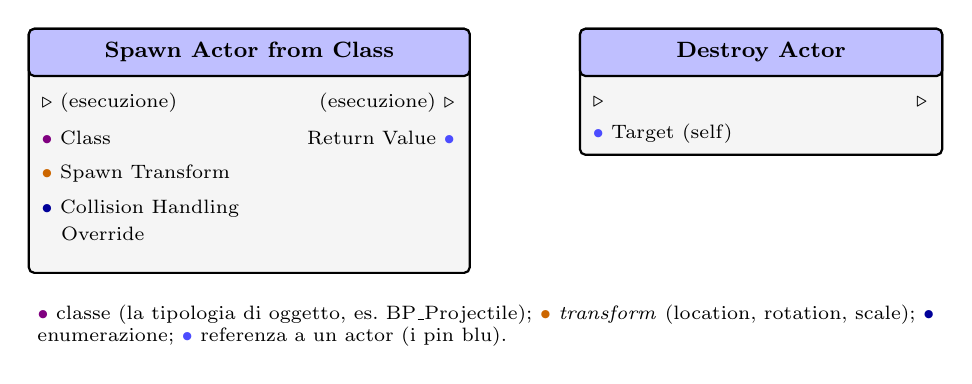
\begin{tikzpicture}[font=\footnotesize,
  ue5hdr/.style={draw, thick, fill=blue!25, minimum width=4.6cm, minimum height=0.6cm,
                 font=\footnotesize\bfseries, rounded corners=2pt},
  ue5bodyb/.style={draw, thick, fill=gray!8, minimum width=4.6cm, rounded corners=2pt},
  ue5pin/.style={font=\scriptsize, anchor=west},
  ue5pino/.style={font=\scriptsize, anchor=east}]
  % --- Spawn Actor from Class
  \node[ue5bodyb, minimum height=3.1cm, minimum width=5.6cm, anchor=north west] (sb)
    at (0,0) {};
  \node[ue5hdr, minimum width=5.6cm, anchor=north west] at (0,0) {Spawn Actor from
    Class};
  \node[ue5pin] at (0.05,-0.95) {$\triangleright$ (esecuzione)};
  \node[ue5pin] at (0.05,-1.4) {\textcolor{violet}{$\bullet$} Class};
  \node[ue5pin] at (0.05,-1.85) {\textcolor{orange!80!black}{$\bullet$} Spawn Transform};
  \node[ue5pin] at (0.05,-2.3) {\textcolor{blue!60!black}{$\bullet$} Collision Handling};
  \node[ue5pin] at (0.3,-2.62) {Override};
  \node[ue5pino] at (5.55,-0.95) {(esecuzione) $\triangleright$};
  \node[ue5pino] at (5.55,-1.4) {Return Value \textcolor{blue!70}{$\bullet$}};
  % --- Destroy Actor
  \node[ue5bodyb, minimum height=1.6cm, anchor=north west] at (7.0,0) {};
  \node[ue5hdr, anchor=north west] at (7.0,0) {Destroy Actor};
  \node[ue5pin] at (7.05,-0.95) {$\triangleright$};
  \node[ue5pin] at (7.05,-1.35) {\textcolor{blue!70}{$\bullet$} Target (self)};
  \node[ue5pino] at (11.55,-0.95) {$\triangleright$};
  % --- legenda
  \node[align=left, font=\scriptsize, anchor=north west, text width=11.4cm] at (0,-3.4)
    {\textcolor{violet}{$\bullet$} classe (la tipologia di oggetto, es.\ BP\_Projectile);
     \textcolor{orange!80!black}{$\bullet$} \emph{transform} (location, rotation,
     scale); \textcolor{blue!60!black}{$\bullet$} enumerazione;
     \textcolor{blue!70}{$\bullet$} referenza a un actor (i pin blu).};
\end{tikzpicture}
\caption{I due nodi della slide sullo spawn: in ingresso la classe da creare, il
\emph{transform} e il modo di gestire le collisioni; in uscita, la referenza all'actor
appena creato. Destroy Actor prende solo l'actor da distruggere. I colori dei pin
seguono le convenzioni dell'editor. Schema ricostruito.}
\label{ue5:fig:spawnnodes}
\end{figure}

\paragraph{Approfondimento: Collision Handling Override.} Il menù a tendina decide che
cosa fare se, nel punto di spawn, l'actor si troverebbe compenetrato con qualcos'altro.
Le opzioni sono: \emph{Default} (usa l'impostazione della classe), \emph{Always Spawn,
Ignore Collisions} (spawna comunque, anche dentro un muro), \emph{Try To Adjust
Location, But Always Spawn} (prova a spostarlo un poco, altrimenti spawna lì),
\emph{Try To Adjust Location, Don't Spawn If Still Colliding} (prova a spostarlo, e se
non trova posto non lo crea) e \emph{Do Not Spawn} (se c'è collisione, niente spawn).
Romero e Sewell (capitolo 3) suggeriscono anche di \textbf{promuovere a variabile} il
Return Value (tasto destro, \emph{Promote to Variable}) se l'oggetto creato servirà più
tardi, per esempio per distruggerlo; prima di usarla, la variabile va controllata con
un \textbf{Is Valid}, perché l'actor potrebbe essere già stato distrutto.

% ---------------------------------------------------------------------
\section{I cicli e il For Loop}
\label{ue5:sec:cicli}

``Anche un'altra cosa che andremo a vedere oggi sarà il \textbf{for loop}. Qualcuno ha
mai sentito parlare di \textbf{cicli} in programmazione?'' Uno studente che ha studiato
il C (``conosco \emph{while}, \emph{do while}, \emph{for}'') dà la definizione: ``è
ripetere un insieme di linee di codice finché una condizione è soddisfatta''. E fa un
esempio sulla torretta: ``finché il player sta in range della torretta, la torretta si
deve muovere; appena esce, quel codice non deve essere più ripetuto''. ``Sì,
assolutamente.''

Oggi, spiega il docente, si costruirà un actor che spawna dei cubetti ``in linea e in
colonne'': ``fondamentalmente andiamo a fare una \textbf{matrice}'', ``come in Excel,
ragazzi: le matrici per righe e colonne''. E lo si farà ``non uno per uno, ma tramite un
\textbf{indice}'': il For Loop è ``un modo iterativo di eseguire il codice fino a che
l'indice, quindi un numero che fa da dire OK, fatto il primo, OK, fatto il secondo, OK,
fatto il terzo\ldots{} Se arrivi a 10, smetti''. I cicli, infine, ``possono essere
innestati: cicli dentro altri cicli'', ed è esattamente ciò che servirà per righe e
colonne.

\paragraph{Approfondimento: i cicli dei Blueprint.} Nei Blueprint i cicli sono nodi di
\emph{flow control}. \textbf{For Loop} ha due ingressi interi, \textbf{First Index} e
\textbf{Last Index}, ed esegue il pin \textbf{Loop Body} una volta per ogni valore
dell'indice, dal primo all'ultimo \emph{compresi}, esponendo il valore corrente sul pin
\textbf{Index}; alla fine esegue \textbf{Completed}. \textbf{For Each Loop} fa lo stesso
scorrendo gli elementi di un array (Romero e Sewell, capitolo 13, lo usano per accendere
tutte le luci di una stanza). \textbf{While Loop} ripete finché una condizione booleana
è vera, come il \emph{while} del C. Una cosa importante, che distingue i cicli dei
Blueprint dal tempo del gioco: un For Loop si esegue \textbf{tutto nello stesso
\emph{frame}}, non ``piano piano nel tempo''. Non può contenere un Delay, e un ciclo
troppo lungo (o un While che non finisce mai) blocca il gioco; Unreal lo interrompe con
un errore di \emph{infinite loop} dopo un numero massimo di iterazioni. Per ripetere
qualcosa nel tempo si usano il Tick o i timer, come la torretta della quarta lezione.

% ---------------------------------------------------------------------
\section{Il fix della torretta: Find Relative Look at Rotation}
\label{ue5:sec:relative}

Prima dei proiettili, ``andremo a fissare una piccola cosa''. Il problema è quello visto
la volta scorsa: la torretta è fatta di tre \emph{static mesh}, e a ruotare è un solo
\emph{componente}, il Pivot, che ruota \textbf{rispetto al suo genitore}, la base. Find
Look at Rotation, invece, ``prenderà la rotazione in confronto a quella del
\textbf{mondo}, cioè di come è posizionato nel mondo''. Finché la torretta non è ruotata
nel livello le due cose coincidono; ma ``io giro la torretta a 90 gradi in engine, e poi
mi fa un offset di 90''.

\paragraph{La scoperta.} ``Ho scoperto, ed è una bellissima cosa, oserei dire, che Unreal
ci mette a disposizione il \textbf{Find Relative Look at Rotation} direttamente.'' Il
nodo ``prende il suo \emph{transform} e ci fa a quel punto un Find Look at Rotation in
relativa''. In pratica, in MoveTurret (il Custom Event chiamato dal timer):
\begin{itemize}
  \item si fa apparire \textbf{Find Relative Look at Rotation} al posto di Find Look at
        Rotation;
  \item al \textbf{Target} si collega quello che c'era già: la posizione del
        bersaglio, Get Actor Location di PlayerTarget;
  \item allo \textbf{Start Transform}, che chiede ``da che \emph{transform}
        partiamo'', si collega \textbf{Get Actor Transform} della torretta;
  \item l'uscita resta splittata, con la sola \textbf{Z} (lo \emph{yaw}) collegata al
        Target di \textbf{RInterp To}: ``questo non cambia assolutamente nulla''.
\end{itemize}
``Facendo ciò, da quel punto in poi la nostra torretta la possiamo ruotare come ci pare.
Tanto lui prenderà sempre a livello relativo.'' Il docente gira la torretta nel livello,
entra nel raggio: ``ecco che ci segue, senza cambiamenti, senza niente''
(figura~\ref{ue5:fig:relative}).

\paragraph{La velocità di interpolazione.} Il docente aveva trasformato l'Interp Speed in
una variabile e ``vi dico già che 0,01 era molto basso. Con questo find relative, ho
messo \textbf{2} e mi va più che bene. È anche più corretto''. A uno studente che non
sapeva come fosse nata la variabile: ``tira fuori dal pin, c'è scritto \emph{Promote to
Variable}''; poi si compila e, in basso a destra, nel \emph{Default Value}, si mette 2.
E, ``intanto'', il \textbf{Delta Time}: ``tira fuori dal Delta Time un pin e fai
\textbf{Get World Delta Seconds}''.

\begin{figure}[htbp]
\centering
\begin{tikzpicture}[font=\footnotesize,
  ue5node/.style={draw, thick, rounded corners=4pt, align=center, fill=gray!8,
                  minimum height=0.85cm, text width=2.4cm},
  ue5event/.style={ue5node, fill=red!12},
  ue5exec/.style={-{Stealth[length=2.5mm]}, very thick, black!80},
  ue5data/.style={-{Stealth[length=2mm]}, thick, blue!60!black},
  ue5trf/.style={-{Stealth[length=2mm]}, thick, orange!80!black},
  ue5flt/.style={-{Stealth[length=2mm]}, thick, green!50!black}]
  \node[ue5event] (mv) at (0,0) {\textbf{Custom Event}\\\textbf{MoveTurret}};
  \node[ue5node] (iv) at (3.1,0) {\textbf{Is Valid}\\PlayerTarget};
  \node[ue5node, text width=2.9cm] (srr) at (11.0,0) {\textbf{Set Relative
    Rotation}\\Target: Pivot};
  \draw[ue5exec] (mv) -- (iv);
  \draw[ue5exec] (iv) -- node[above, font=\scriptsize]{Is Valid} (srr);
  % dati
  \node[ue5node, fill=orange!12] (gat) at (0,-2.2) {\textbf{Get Actor
    Transform}\\(self)};
  \node[ue5node] (gal) at (0,-3.6) {\textbf{Get Actor Location}\\di PlayerTarget};
  \node[ue5node, text width=3.0cm, fill=yellow!20] (frl) at (3.6,-2.9)
    {\textbf{Find Relative Look at Rotation}\\Start Transform\\Target};
  \node[ue5node, text width=2.8cm] (ri) at (7.4,-2.9) {\textbf{RInterp To}\\
    Current: Get Relative Rotation (Pivot)\\Target: solo Z};
  \node[ue5node] (gwd) at (7.4,-5.0) {\textbf{Get World Delta Seconds}};
  \node[ue5node] (spd) at (4.1,-5.0) {\textbf{InterpSpeed}\\(variabile, 2)};
  \draw[ue5trf] (gat) -- (frl);
  \draw[ue5data] (gal) -- (frl);
  \draw[ue5flt] (frl) -- node[above, font=\scriptsize]{Z} (ri);
  \draw[ue5flt] (gwd) -- node[right, font=\scriptsize]{Delta Time} (ri);
  \draw[ue5flt] (spd) -- node[below, font=\scriptsize, pos=0.7]{Interp Speed} (ri);
  \draw[ue5flt] (ri.east) -| (srr.south);
\end{tikzpicture}
\caption{MoveTurret dopo il \emph{fix}. Il nodo nuovo (in giallo) calcola la rotazione
verso il bersaglio nello spazio della torretta, a partire dal suo \emph{transform}:
la torretta si può girare nel livello senza offset. Delta Time viene ora da Get World
Delta Seconds e l'Interp Speed, promosso a variabile, vale 2. Schema ricostruito.}
\label{ue5:fig:relative}
\end{figure}

\paragraph{Lo studente con la torretta che non gira.} Il primo caso in condivisione è
quello di uno studente che ha perso le lezioni precedenti per un problema al computer.
Il pivot non era stato reimportato a $-113$ (``non me l'ha fatto fare'', il re-import
non partiva). Lo si reimporta trascinando il file del materiale didattico nel
\emph{Content Browser} (attenzione a non lasciarlo cadere sopra altre cartelle); poi, in
scena, il pivot è ``storto'': lo si raddrizza con la modalità \textbf{Modeling}
(\textbf{Shift+5}), strumento \textbf{XForm}, \emph{Edit Pivot}. Nel Blueprint il pivot è
``un po' interrato'', e il cannone va staccato e riattaccato. Alla fine ruota, ``c'è un
piccolo offset, ma è importante che ruoti'', e punta ``dall'altra parte'': il caso è
rimandato alla pausa (sezione~\ref{ue5:sec:pausa}).

\paragraph{Approfondimento: perché il nodo nuovo risolve.} Find Relative Look at
Rotation (\emph{Start Transform}, \emph{Target Location}) trasforma prima il punto
bersaglio nello spazio locale del \emph{transform} di partenza, e poi calcola la
rotazione per guardarlo da lì. Il risultato è quindi già una rotazione
\textbf{relativa} all'actor, la stessa grandezza che Set Relative Rotation imposta sul
Pivot: i due spazi, che nel grafo della quarta lezione erano mescolati, ora coincidono.
Restano due avvertenze. Il punto di partenza è l'origine dell'actor, la base: va bene
per lo \emph{yaw}, ma per un \emph{pitch} preciso converrebbe partire dal
\emph{transform} del Pivot o del cannone (Get World Transform sul componente). E l'offset
dovuto alla \emph{mesh} reimportata a 113 gradi resta: il nodo presuppone che la
torretta, a rotazione zero, guardi lungo la propria X. Quanto alla velocità: con Delta
Time preso da Get World Delta Seconds e Interp Speed 2, il prodotto è circa 0,02 a 100
\emph{frame} al secondo, e la torretta insegue in modo morbido e uguale su ogni
macchina, come anticipato nella lezione precedente.

% ---------------------------------------------------------------------
\section{I trace: linee immaginarie}
\label{ue5:sec:trace}

``Abbiamo parlato di spawn, ma anche una cosa che andremo a vedere è chiamata
\textbf{line trace}.'' ``Oggi usiamo lo \textbf{sphere trace}, però in generale un trace
è una \textbf{linea immaginaria} che viene fatta dall'engine'' per scoprire che cosa c'è
lungo un percorso.

\paragraph{La dimostrazione.} Il docente lo mostra con la torretta che aveva già
preparato (``ecco qua, spawnano la marea di proiettili''). Entrando nel raggio, davanti
al cannone compare un \textbf{reticolo rosso}: ``una linea immaginaria, che non vedremo
se dovessimo avere un eseguibile''. Ma ``vedete che è rosso, rosso, rosso; se
\emph{overlappa}, diventa \textbf{verde}. Dice: ah, ho visto qualcosa! E quindi comincia
a sparare''. Poi, per confronto, trasforma al volo lo sphere trace in un \textbf{Line
Trace by Channel}: ``facciamo una linea''. All'inizio la linea non trova nulla, ``perché
è impostata male''; basta cambiarle il canale, e ``ecco che ci ha trovato'': ``fa rosso
il puntino e verde. Dice: ah, ok, ti ho beccato''.

\paragraph{A che cosa servono.} ``Sono delle linee immaginarie che servono a noi
\emph{developer} per dire: oh, c'è qualcosa che overlappa una linea invisibile?
Effettivamente sì, effettivamente no.'' Il docente racconta di averle usate per
un'intelligenza artificiale: ``tracciavo una linea tra me e il player; se c'era qualcosa
di mezzo, vuol dire che non lo vedeva; se invece non c'era niente, vuol dire che lo
vedeva''. È ``proprio una \textbf{linea di vista}''. E un avvertimento, ripetuto:
``non esagerate con il trace, perché anche esso è molto pesante'', tanto più se, come
oggi, lo si fa a ogni \emph{frame}.

\paragraph{Approfondimento: le famiglie di trace.} Romero e Sewell (capitolo 14)
definiscono i trace come test di collisione lungo un segmento. Ne esistono di due
tipi di ``filtro'': \textbf{by Channel}, che cercano gli oggetti che bloccano un
\emph{trace channel} (Visibility, Camera o un canale creato da noi), e \textbf{for
Objects}, che cercano gli oggetti di certi \emph{object type} (WorldStatic,
WorldDynamic, Pawn, PhysicsBody, Vehicle, Destructible). E di quattro forme: la
\textbf{linea}, la \textbf{sfera}, la \textbf{capsula} e il \textbf{box}, dove le forme
``spesse'' sono più costose della linea. Infine, ogni trace ha una versione singola,
che restituisce il primo oggetto colpito, e una \textbf{Multi}, che li restituisce
tutti (sezione~\ref{ue5:sec:errori}). Tutti hanno gli stessi ingressi principali:
\textbf{Start} ed \textbf{End}, il canale o i tipi, \textbf{Trace Complex} (testare
contro la \emph{mesh} vera o contro le forme di collisione semplificate), \textbf{Actors
to Ignore}, \textbf{Draw Debug Type} e \textbf{Ignore Self}. Le uscite sono un
\textbf{Out Hit} (una struttura \emph{Hit Result} con, tra l'altro, il punto d'impatto,
la normale della superficie e l'actor colpito, leggibili con \emph{Break Hit Result}) e
un \textbf{Return Value} booleano: vero se qualcosa ha bloccato il trace.

% ---------------------------------------------------------------------
\section{L'evento Shoot e i vettori del trace}
\label{ue5:sec:shoot}

``La prima cosa è che dobbiamo creare un evento \textbf{Shoot}'': un \textbf{Custom
Event} nel grafo di BP\_Turret.

\paragraph{Is Valid, per buona maniera.} ``Intanto la prima cosa che andiamo a fare è
vedere se esiste il target'': un \textbf{Is Valid} (``la macro con il punto
interrogativo'') su PlayerTarget. ``È buona maniera fare questa cosa, di vedere se
effettivamente esiste o non esiste, perché ci ottimizza i processi'': se non c'è un
bersaglio, non si esegue nulla. (Più avanti, nella sezione~\ref{ue5:sec:bocche}, questo
Is Valid verrà spostato fuori da Shoot.)

\paragraph{Lo Sphere Trace by Channel.} Poi lo \textbf{Sphere Trace by Channel}: ``una
linea immaginaria che andremo a creare in modo tale che, se il nostro character entra in
questa sfera, vuol dire che io lo sto vedendo ed è in puntamento''. Che cosa chiede?
``Un punto di \textbf{Start} e un punto di \textbf{End}'', con i pin
\textbf{gialli}. ``Chi si ricorda quali sono gli elementi gialli in Unreal?'' ``Un
vettore.'' ``Bravissimo, è un vettore. In questo caso, un vettore di locazione'': una X,
una Y e una Z.

\paragraph{Il punto di partenza: TraceSpawn.} Il trace deve partire ``più o meno dalla
canna, da questo punto qua in avanti''. Si potrebbe usare la posizione del Pivot, ``però
vi dico che è più corretto fare una cosa del genere: andiamo a creare proprio un
\textbf{punto vuoto}'' dedicato. Nei componenti si fa \emph{Add} e si scrive
\textbf{Scene}: un \emph{Scene Component}, ``solo un punto nello spazio'', senza
\emph{mesh} né collisioni. Lo si \textbf{attacca al cannone}, lo si posiziona ``in
mezzo alle due canne'', e lo si rinomina (``per rinominare le cose molto più
velocemente: cliccate sull'elemento, \textbf{F2}, e scrivete'') in
\textbf{TraceSpawn}. ``L'abbiamo attaccato al cannone perché il pivot fa ruotare il
cannone e il cannone farà ruotare il TraceSpawn: c'è questa \textbf{dipendenza a
cascata}.'' Dal componente TraceSpawn si prende \textbf{Get World Location}, ``dove è
posizionato nel mondo'', e la si collega allo \textbf{Start}.

\paragraph{Il punto d'arrivo: il forward vector.} ``Ci manca quello del punto di fine.
Dove deve arrivare?'' Qui torna la teoria dei vettori della quarta lezione. Ogni
\emph{mesh}, ogni componente, ogni actor ha dei vettori di direzione ``già prefatti'':
\begin{itemize}
  \item \textbf{Get Actor Forward Vector}, che ``punterà sempre in avanti'';
  \item \textbf{Get Actor Right Vector}, ``che punterà sempre a destra'';
  \item \textbf{Get Actor Up Vector}, ``che punterà sempre in alto'',
\end{itemize}
sempre relativi all'oggetto. ``Domanda: se io moltiplicassi per $-1$ il forward vector,
dove punterà rispetto alla mesh?'' ``Dietro.'' ``Bravissimo'': moltiplicare per $-1$
``inverte il risultato''; così si ottengono il \emph{back} vector, la sinistra e il
basso.

\paragraph{Lungo 1: moltiplicare.} Ma se si collega il forward vector così com'è ``non ci
darà assolutamente nulla, perché è molto piccolo'': ``il forward vector che ci dà Unreal
è di \textbf{lunghezza 1}'', un vettore normalizzato. ``Buona prassi è prenderlo e
moltiplicarlo, per esempio per \textbf{800}'': ``avremo un vettore 800 volte più
lungo''. (Uno studente non riesce a scrivere 800 nel Multiply: ``il pallino è giallo e
non verde''. ``Se moltiplicate un vettore, vi dà direttamente la moltiplicazione per un
altro vettore, ma potete cambiare il secondo fattore: tasto destro, \emph{To Float}.
Diventerà verde, e ci mettete 800.'')

\paragraph{Un punto non è una linea: sommare.} ``Magari vi verrebbe da dire: ok, ho
trovato il punto laggiù, lo vado a mettere nell'End. No, ancora no.'' Il forward vector
moltiplicato è ``un punto, non è una linea'': è uno spostamento di 800 in avanti,
calcolato come se si partisse dall'origine del mondo. ``Per farlo diventare una linea
dobbiamo letteralmente \textbf{sommare} due vettori'': la World Location di TraceSpawn
più il forward vector per 800. ``È un discorso che sembra strano, però effettivamente
quello che abbiamo qua è solo un punto nello spazio; con la somma ne traiamo un'effettiva
linea'' (figura~\ref{ue5:fig:vettori}).

\paragraph{Il forward vector giusto.} Alla prima prova il trace c'è, ma ``non segue il
pivot'': resta fermo mentre la torretta ruota. Il motivo: Get \emph{Actor} Forward
Vector è il vettore dell'actor intero, cioè della \textbf{base}, ``quindi sarà sempre lì.
Non girerà, perché deve girare insieme al cannone''. La correzione: ``invece di prendere
il Get Actor Forward Vector, prendiamo il \textbf{Get Forward Vector del TraceSpawn}''.
(``A me non fa collegare TraceSpawn e Get Forward Vector'': bisogna tirare il filo
\emph{dal} componente TraceSpawn e cercare \emph{Get Forward Vector}, la versione per i
componenti.)

\begin{figure}[htbp]
\centering
\begin{tikzpicture}[font=\footnotesize, >={Stealth[length=2.5mm]}]
  % assi del mondo
  \draw[->, thick, gray] (-0.3,0) -- (2.0,0) node[right]{X};
  \draw[->, thick, gray] (0,-0.3) -- (0,1.8) node[above]{Y};
  \node[below left, gray, font=\scriptsize] at (0,0) {origine del mondo};
  % torretta vista dall'alto
  \coordinate (C) at (6.0,0.4);
  \fill[gray!25, draw=black, thick] (C) circle (0.7);
  \node[font=\scriptsize, below] at ($(C)+(0,-0.7)$) {base};
  \begin{scope}[rotate around={35:(C)}]
    \fill[orange!25, draw=black, thick] ($(C)+(0,-0.2)$) rectangle ($(C)+(1.3,0.2)$);
  \end{scope}
  \coordinate (S) at ($(C)+(35:1.15)$);
  \fill[blue!60] (S) circle (0.07);
  \node[font=\scriptsize, align=center] at ($(S)+(-0.9,0.55)$) {TraceSpawn\\(Start)};
  % vettore posizione
  \draw[->, very thick, blue!60!black] (0,0) -- (S) node[pos=0.45, below, sloped,
    font=\scriptsize] {Get World Location};
  % forward unitario all'origine
  \draw[->, very thick, red!70!black] (0,0) -- (35:0.8);
  % forward x 800 all'origine (punto sbagliato)
  \draw[->, thick, red!70!black, dashed] (0,0) -- (35:3.6);
  \fill[red!70!black] (35:3.6) circle (0.06);
  \node[red!70!black, font=\scriptsize, align=left, anchor=south east] at (35:3.6)
    {Forward $\times$ 800\\(da solo: un punto\\vicino all'origine)};
  \node[red!70!black, font=\scriptsize, anchor=north west] at (0.15,-0.25)
    {Forward: lunghezza 1};
  % fine = start + forward x 800
  \coordinate (E) at ($(S)+(35:3.6)$);
  \draw[->, very thick, green!45!black] (S) -- (E);
  \fill[green!45!black] (E) circle (0.07);
  \node[right=3pt, green!45!black, align=left] at (E) {End =\\Start + Forward
    $\times$ 800};
  % sfera del trace
  \foreach \t in {0.2,0.45,0.7,0.95} {
    \draw[green!45!black, thin] ($(S)!\t!(E)$) circle (0.32);
  }
  \node[green!45!black, font=\scriptsize, anchor=west] at ($(S)!0.5!(E)+(0.45,-0.3)$)
    {Sphere Trace, Radius 80};
\end{tikzpicture}
\caption{I vettori del trace, visti dall'alto. Get World Location di TraceSpawn è un
vettore dall'origine del mondo al punto di partenza. Il Forward Vector è lungo 1;
moltiplicato per 800 diventa uno spostamento, che però, preso da solo, indica un punto
vicino all'origine (tratteggio). Sommato alla posizione di partenza, dà la fine giusta:
800 unità davanti alla canna. Lo sphere trace ``trascina'' una sfera di raggio 80 lungo
il segmento. Schema ricostruito, non in scala.}
\label{ue5:fig:vettori}
\end{figure}

\paragraph{Il raggio e il debug.} Due dettagli ancora. Il \textbf{Radius} dello sphere
trace parte da zero: ``il raggio della nostra bellissima sfera sarà zero, quindi non
esisterà''. Il docente mette \textbf{80}. E per vedere il trace in editor, ``lo vedremo
solo noi \emph{developer}'', c'è \textbf{Draw Debug Type}, da impostare su \textbf{For
One Frame}: ``perché se adesso la mettiamo \emph{For Duration}, ha una durata, sarà un
casino, perché lo fa ogni \emph{frame}'' (tabella~\ref{ue5:tab:debug}). Per provarlo,
Shoot viene chiamato dall'\textbf{Event Tick} (``prendete il Tick, scrivete Shoot,
come avete chiamato questo evento''): ``giusto per vedere effettivamente che
funzioni''.

\begin{table}[htbp]
\centering
\small
\begin{tabular}{@{}p{3.0cm}p{11.0cm}@{}}
\toprule
\textbf{Draw Debug Type} & \textbf{Che cosa disegna} \\
\midrule
None & niente: il trace c'è, ma non si vede (il valore di default) \\
For One Frame & il trace per un solo \emph{frame}: se il trace è chiamato a ogni
\emph{frame}, si vede ``in diretta''; è l'opzione usata a lezione \\
For Duration & il trace resta visibile per un certo tempo (Draw Time, nei dettagli del
nodo): chiamato a ogni \emph{frame}, accumula centinaia di disegni sovrapposti \\
Persistent & il trace resta disegnato per sempre: utile per un trace singolo, da
esaminare con calma \\
\bottomrule
\end{tabular}
\caption{Le opzioni di Draw Debug Type dei nodi di trace. I colori del disegno sono il
rosso per il tratto libero e il verde dal punto in cui il trace è stato bloccato (Trace
Color e Trace Hit Color, modificabili nel nodo).}
\label{ue5:tab:debug}
\end{table}

\paragraph{I problemi del momento.} Le condivisioni mostrano errori ricorrenti: lo
Start e l'End scambiati o collegati senza la somma (``Start è questo, solo questo; lo
attacchi così; il più va nell'End''); Draw Debug Type lasciato su \emph{None}; Shoot non
chiamato dal Tick (``l'hai messo sul Tick? Ah, no. Metti l'evento Shoot sul Tick''); e
la linea che compare ma non ruota con il cannone, per il motivo visto sopra.

% ---------------------------------------------------------------------
\section{I trace channel e le risposte di collisione}
\label{ue5:sec:canali}

Ora il trace c'è e ruota, ``ma come potete vedere non abbiamo il verdino, non ci dice
\emph{ho trovato}'': il player ci passa attraverso senza essere visto. Il motivo è il
\textbf{trace channel}. ``Di standard Unreal ci dà due canali, che sono
\textbf{Visibility} e \textbf{Camera}''; quello del docente (``questo qua al testo lo
vedete, l'ho creato io'') è un canale \textbf{custom}, che risponde ``in una certa
maniera, dipendentemente da certe opzioni''. Bisogna crearlo.

\paragraph{Creare il canale.} Dal menù \textbf{Edit}, \textbf{Project Settings}; si scende
``giù giù giù giù'' fino a \textbf{Collision} (nella sezione \emph{Engine}). Lì,
\textbf{New Trace Channel}: ``lo chiamate come volete, lo chiamiamo magari
\textbf{DetectionTurret}'', con \textbf{Default Response} su \textbf{Ignore}. Che cosa
vuol dire? ``Guarda questo trace: in risposta a tutti gli altri elementi in cui può
collidere, cosa fa di base? Ignora tutto, perché è meglio che ignori tutto, in modo tale
che tanto deve trovare solo il player.'' Se si mettesse \emph{Block}, ``ci bloccherebbe
tutto quanto'', e bisognerebbe togliere il blocco a tutti gli elementi statici e
dinamici. ``È più facile mettere ignora tutto, e poi mettiamo il \emph{tick} positivo al
nostro player.''

\paragraph{Il player risponde Block.} Si apre il \textbf{Third Person Character}, si
seleziona la \textbf{Mesh} e si cerca \emph{Collision} nei dettagli (``importante che, se
non avete compilato, compilate, perché se no non vi apparirà mai il nostro
DetectionTurret''). I \textbf{Collision Presets} sono grigi, perché è attivo un
\emph{preset}: si sceglie \textbf{Custom} dalla tendina, e nella riga di DetectionTurret
si mette la spunta su \textbf{Block}. ``In che modo reagisci al trace channel della
nostra torretta? Overlap, Block, Ignore. In questo caso andiamo a fare che blocca.''

\paragraph{Ignore, Overlap, Block.} Il docente ripassa le tre risposte con le mani:
``questa è la mia mano, l'oggetto 1, l'oggetto 2''. Con l'\textbf{Overlap}, ``se si
toccano non c'è una collisione fisica, quindi volendo si trapassano'', ma ``c'è una
\emph{detection}: l'engine dice, sono loro che collidono, quindi c'è un segnale''; è ciò
che si usa ``per i blocchi invisibili''. Il \textbf{Block}, invece, ``è proprio un
blocco fisico''. Il trace non ha un corpo, quindi per lui il Block è ``semplicemente
un'accortezza'': ``ehi, ho trovato il player, mi blocco''; ed è grazie al blocco che
appare la sfera ``parte verde, parte rossa'' (tabella~\ref{ue5:tab:risposte}).

\begin{table}[htbp]
\centering
\small
\begin{tabular}{@{}p{2.0cm}p{5.6cm}p{6.4cm}@{}}
\toprule
\textbf{Risposta} & \textbf{Tra due corpi} & \textbf{Per un trace} \\
\midrule
Ignore & si attraversano e nessuno se ne accorge & l'oggetto è invisibile per quel
trace \\
Overlap & si attraversano, ma scatta un evento di \emph{overlap} (i ``blocchi
invisibili'', la sfera della torretta) & il trace lo registra ma prosegue: lo vede solo
un trace Multi, e il Return Value resta falso \\
Block & si fermano l'uno contro l'altro: collisione fisica & il trace si ferma lì: è un
\emph{hit}, il disegno di debug diventa verde e il Return Value è vero \\
\bottomrule
\end{tabular}
\caption{Le tre risposte di collisione. Ogni componente dichiara una risposta per ogni
canale (Visibility, Camera, i canali custom) e per ogni \emph{object type}; quando due
oggetti si incontrano, vale la risposta più ``debole'' delle due.}
\label{ue5:tab:risposte}
\end{table}

\paragraph{Scegliere il canale nel trace.} Tornati in BP\_Turret, nello Sphere Trace by
Channel di Shoot si apre la tendina \textbf{Trace Channel}: ``c'è Visibility, Camera e
DetectionTurret''. Se compaiono solo Visibility e Camera, ``vai con \textbf{Compile},
qui in alto a sinistra''. In Play: ``vedete che è diventato verde. C'è il trace rosso,
viene bloccato, e da lì in poi c'è quello spazio verde'': ``è da lì in poi che il nostro
player è presente''. Avvicinandosi, il tratto verde si allunga.

\paragraph{Il Return Value.} Infine un \textbf{Print String} collegato al
\textbf{Return Value} del trace, ``che ci dice letteralmente: hai preso qualcosa? Sì,
no''. È un \textbf{booleano}: falso se non ha trovato niente, vero se ha trovato
qualcosa. In Play ``spunteranno un botto di true e false, ma è normale, sta sul Tick'':
``false, false, false\ldots{} true, true, true''.

\paragraph{Approfondimento: Mesh o Capsule?} A lezione la risposta Block al canale
DetectionTurret viene data alla \textbf{Mesh} del personaggio, e funziona. Nel Third
Person Character, però, il componente che rappresenta il corpo ai fini delle collisioni
è la \textbf{Capsule Component}, la radice; la Mesh scheletrica, di default, usa un
\emph{preset} (\emph{CharacterMesh}) pensato per non interferire con il movimento. Dare
il Block alla Mesh significa che il trace colpisce la forma del personaggio, con le sue
parti fisiche; darlo alla capsula significa colpire un cilindro più semplice. Entrambe
le scelte sono legittime; l'importante è sapere quale si è fatta, perché l'\emph{Hit
Actor} sarà lo stesso, ma l'\emph{Hit Component} e il punto d'impatto no.

% ---------------------------------------------------------------------
\section{Il proiettile: BP\_Projectile e il Projectile Movement}
\label{ue5:sec:proiettile}

``Abbiamo fatto la torretta che gira, abbiamo fatto la torretta che detecta: adesso
dobbiamo far sparare.'' Un Custom Event \textbf{SpawnProjectile}, ``ma che succede,
ragazzi? Non abbiamo un proiettile''. Lo si crea: tasto destro nel Content Browser,
\textbf{Blueprint Class}, \textbf{Actor}, e lo si chiama \textbf{BP\_Projectile}.

\paragraph{Due actor, due compiti.} Perché un Blueprint a parte, e non tutto dentro la
torretta? ``Due actor, uno che fa un compito e uno che fa un altro, è il miglior modo
per gestire i comportamenti.'' ``Perché a un certo punto magari vi arriva un
\emph{designer} e vi dice: ragazzi, non voglio che spawni più i proiettili, voglio che
spawni \textbf{banane}. Eh, se l'avete fatto dentro la torretta dovete fare un casino.
Invece, cambiare semplicemente il proiettile è molto più facile.''

\paragraph{La mesh.} Il proiettile è ``formato da due cose''. La prima è una \textbf{Static
Mesh}, rinominata \textbf{MeshProjectile}: una \textbf{sfera} di default (``se volete,
potete scaricare un modello, così ci mettete un proiettile al posto della palla'').
La si scala a \textbf{0,5}, poi a \textbf{0,3} (``mi sembra un po' grandicello''),
con il \textbf{lucchetto} della scala chiuso. ``Questo lucchetto l'abbiamo spiegato alla
prima lezione'': aperto, permette di modificare gli assi uno per uno; chiuso, ``se
modificate un singolo asse, vi scalerà anche le altre, in modo tale che rimangano
uniformi, perché sennò vengono forme stiracchiate''. Come materiale, \textbf{MI\_Solid\_Blue}
(``mi solid blue'').

\paragraph{Il Projectile Movement.} La seconda cosa è il movimento. ``Unreal ci arriva
con un regalo incredibile'': come la volta scorsa c'era il Rotating Movement per il
mulino, ``arriva la possibilità di avere un \textbf{Projectile Movement}, per quanti
giochi ormai hanno dei proiettili''. Si aggiunge il componente, e nei dettagli ci sono
``un sacco di dati in cui possiamo giocare'': ``tanti giochi ai giorni d'oggi hanno cose
molto comuni. Quanti FPS ce ne sono? Anche le armi di \emph{Borderlands}, che sono tutte
strane, alla base si parla sempre di sparare''. I valori della lezione:
\begin{itemize}
  \item \textbf{Initial Speed} 1000 e \textbf{Max Speed} 1000 (per guardarlo meglio, a
        un certo punto l'Initial Speed scende a 100, ``la lumaca'', e poi torna a 1000,
        ``una velocità da proiettile'');
  \item \textbf{Projectile Gravity Scale} a \textbf{0}: ``questo proiettile al momento
        è afflitto dalla gravità''; ``noi vogliamo che vada dritto per dritto'';
  \item \textbf{Velocity} lasciata a $(1, 0, 0)$: ``la velocità è la direzione'',
        quindi ``è 1 sull'asse X'', e il proiettile ``andrà dritto così''.
\end{itemize}
E la mesh deve essere \textbf{Movable}, ``se no vi danno errore''. Messo in scena e
avviato il Play, ``il nostro bellissimo proiettilino se ne va per la sua'' strada:
attraversa tutto, ``overlapperà, e chissà chi lo vedrà più''. (A una studentessa la
pallina ``cade semplicemente'': aveva lasciato la gravità a 1.)

\paragraph{Approfondimento: i parametri del Projectile Movement.} Romero e Sewell
(capitolo 6) modificano il proiettile del modello \emph{First Person} con gli stessi
parametri. \textbf{Initial Speed} è la velocità con cui il proiettile parte; \textbf{Max
Speed} è il limite, che conta solo se qualcos'altro lo accelera (un razzo con il motore
acceso); per un proiettile d'arma ha senso che le due coincidano. \textbf{Velocity} è
una direzione nello spazio \emph{locale} del proiettile: se Initial Speed è maggiore di
zero, Unreal ne usa solo la direzione e la moltiplica per l'Initial Speed. Per questo
è importante che lo spawn dia al proiettile la rotazione giusta: la X locale del
proiettile deve guardare fuori dalla canna. \textbf{Projectile Gravity Scale} moltiplica
la gravità del mondo (0 nessuna, 0,1 ``proiettile leggero''). La sezione \textbf{Projectile
Bounces}, con \emph{Should Bounce}, decide se rimbalza sui muri; e \textbf{Rotation Follows
Velocity} lo fa girare nella direzione del moto, utile per frecce e razzi.

% ---------------------------------------------------------------------
\section{Il proiettile che si distrugge}
\label{ue5:sec:distruzione}

``Noi vorremmo che il nostro proiettile sia molto più realistico: trova un muro e
scompare.'' E non è solo estetica: ``immaginatevi che adesso spawneremo dei proiettili
che andranno nell'infinito e oltre''; l'engine ``dirà: guarda, esiste'', e ``non
libereremo mai la memoria''.

\paragraph{Un trace attorno al proiettile.} La soluzione riusa il trace: nell'\textbf{Event
Tick} di BP\_Projectile, uno \textbf{Sphere Trace by Channel} di raggio \textbf{30},
``una sfera intorno al nostro proiettile che ci dirà: guarda, hai colpito qualcosa?''.
Start ed End sono \textbf{lo stesso punto}, \textbf{Get Actor Location} del proiettile:
``vogliamo che l'inizio e la fine siano lo stesso punto''. Con Draw Debug Type su For
One Frame, ``intorno alla nostra pallina si è creato un trace''.

\paragraph{Branch e Destroy Actor.} Poi: ``molto semplicemente, Return Value è vero? Sì?
Allora distruggete''. Un \textbf{Branch} (``tenete premuto B e cliccate'') sul Return
Value, e sul ramo True un \textbf{Destroy Actor} (figura~\ref{ue5:fig:proiettile}). In
Play, alla ``velocità della lumaca'', il proiettile arriva al muro e sparisce: ``si è
distrutto, quindi abbiamo il comportamento di base''. Il Tick, nota il docente,
``inizierà solamente quando l'oggetto esiste'': ogni proiettile controlla sé stesso
finché vive.

\begin{figure}[htbp]
\centering
\begin{tikzpicture}[font=\footnotesize,
  ue5node/.style={draw, thick, rounded corners=4pt, align=center, fill=gray!8,
                  minimum height=0.85cm, text width=2.5cm},
  ue5event/.style={ue5node, fill=red!12},
  ue5exec/.style={-{Stealth[length=2.5mm]}, very thick, black!80},
  ue5vec/.style={-{Stealth[length=2mm]}, thick, yellow!50!black},
  ue5bool/.style={-{Stealth[length=2mm]}, thick, red!60!black},
  ue5comp/.style={draw, thick, rounded corners=3pt, minimum width=3.5cm,
                  minimum height=0.55cm, align=center, font=\scriptsize}]
  % componenti
  \node[font=\scriptsize\bfseries] at (0,1.0) {BP\_Projectile: componenti};
  \node[ue5comp, fill=gray!20] (r) at (0,0.4) {DefaultSceneRoot};
  \node[ue5comp, fill=blue!20] (m) at (0.6,-0.3) {MeshProjectile (sfera, 0,3)};
  \node[ue5comp, fill=green!15] (pm) at (0,-1.0) {ProjectileMovement};
  \draw[thick, gray!60!black] ([xshift=-1.5cm]r.south) |- (m.west);
  \node[font=\scriptsize, align=left, anchor=west] at (-1.45,-1.75)
    {Initial / Max Speed 1000\\Gravity Scale 0, Velocity (1,0,0)};
  % grafo
  \node[ue5event] (tick) at (4.4,0.2) {\textbf{Event Tick}};
  \node[ue5node, text width=3.0cm] (st) at (7.9,0.2) {\textbf{Sphere Trace by
    Channel}\\Radius 30\\Channel: ProjectileTrace\\Debug: For One Frame};
  \node[ue5node, text width=1.6cm] (br) at (11.3,0.2) {\textbf{Branch}};
  \node[ue5node, text width=1.9cm] (de) at (11.3,-1.9) {\textbf{Destroy Actor}\\(self)};
  \node[ue5node] (gal) at (4.4,-1.6) {\textbf{Get Actor Location}\\(self)};
  \draw[ue5exec] (tick) -- (st);
  \draw[ue5exec] (st) -- (br);
  \draw[ue5exec] (br) -- node[right, font=\scriptsize]{True} (de);
  \draw[ue5vec] (gal.east) -| node[pos=0.75, left, font=\scriptsize, align=right]
    {Start\\e End} (st.south);
  \draw[ue5bool] ([yshift=-0.4cm]st.east) -- node[above, font=\scriptsize, pos=0.4]
    {Return Value} ([yshift=-0.4cm]br.west);
\end{tikzpicture}
\caption{Il proiettile. A sinistra i componenti: una sfera scalata e il Projectile
Movement, che fa tutto il moto. A destra il grafo: a ogni \emph{frame}, una sfera di
raggio 30 attorno al proiettile (Start ed End coincidono); se qualcosa la blocca, il
proiettile si distrugge. Il canale, all'inizio Visibility e poi Camera, diventa alla
fine ProjectileTrace. Schema ricostruito.}
\label{ue5:fig:proiettile}
\end{figure}

\paragraph{Approfondimento: altri modi di distruggere un proiettile.} Il trace sul Tick
funziona ed è istruttivo, ma non è l'unico modo, né il più economico. Il Projectile
Movement ha un proprio evento, \textbf{On Projectile Stop}, che scatta quando il
proiettile si ferma contro qualcosa che lo blocca; e un componente di collisione (una
Sphere Collision come radice del proiettile, con il Projectile Movement che la muove)
genera \textbf{Event Hit} o \textbf{On Component Hit} all'impatto. Romero e Sewell
(capitolo 6) collegano proprio all'evento di \emph{hit} il Destroy Actor, ``così che il
proiettile venga sempre distrutto quando collide''. Infine, per i proiettili che non
colpiscono nulla, l'actor ha una proprietà \textbf{Initial Life Span} (nei \emph{Class
Defaults}): se maggiore di zero, l'actor si distrugge da solo dopo quei secondi. È una
rete di sicurezza contro i proiettili che vanno ``nell'infinito e oltre''.

% ---------------------------------------------------------------------
\section{Visibility, Camera e il canale ProjectileTrace}
\label{ue5:sec:projtrace}

Il proiettile si distrugge contro il muro, ``anche il player, volendo?'' No: ``mi metto
davanti, e infatti non ce lo prende''. Con il canale \textbf{Visibility} il personaggio
non viene visto; cambiando il canale in \textbf{Camera}, ``così ci prende pure il
player''.

\paragraph{Perché.} Il docente apre le collisioni del Third Person Character: c'è la
tabella delle \textbf{Collision Responses}, con Ignore, Overlap e Block, e sotto le
\textbf{Trace Responses}, ``cioè come rispondo a questo trace''. ``Come rispondo al trace
Visibility? Vedete che c'è la spunta su Ignore; invece il Camera viene bloccato.''
``Semplicemente è un concetto di collisioni.''

\paragraph{Un canale per il proiettile.} ``Lo facciamo, ragazzi, così almeno è buona
prassi'': un secondo canale, \textbf{ProjectileTrace}. Qui il ragionamento è opposto a
quello di DetectionTurret. Il docente prima pensa a Ignore e a mettere il Block sui
quattro muri uno per uno (``però è più pesante''), poi cambia idea: ``è molto meglio
farlo in \textbf{Block}, così facciamo un Block e leviamo semplicemente quelli che non ci
interessano''. La regola generale: ``quante cose ho che devono bloccare, e quante che
devono ignorare?''. Il proiettile ``sbatte praticamente con tutto'', quindi Default
Response \textbf{Block}, e si escludono le poche eccezioni (tabella~\ref{ue5:tab:canali}):
\begin{itemize}
  \item il \emph{character}: Block (``va benissimo'');
  \item la \textbf{Sphere} della torretta, il raggio d'azione: Custom, ProjectileTrace
        su \textbf{Ignore}, altrimenti il proiettile esploderebbe appena nato, dentro la
        sfera;
  \item anche \textbf{Pivot}, \textbf{Base} e \textbf{Cannon}: ``non vogliamo che
        rimbalzi contro la stessa torretta che l'ha sparato'', quindi Custom e Ignore
        a tutti e tre.
\end{itemize}
Nel trace del proiettile si sceglie ProjectileTrace (``sempre compilato, perché se no non
vi arriva''), e in Play il proiettile si distrugge sia sul player sia sul muro.

\begin{table}[htbp]
\centering
\small
\begin{tabular}{@{}p{2.8cm}p{2.1cm}p{9.1cm}@{}}
\toprule
\textbf{Canale} & \textbf{Default} & \textbf{Eccezioni impostate a lezione} \\
\midrule
DetectionTurret & Ignore & Mesh del Third Person Character: \textbf{Block}. Il trace
della torretta vede solo il giocatore. \\
ProjectileTrace & Block & Sphere, Pivot, Base e Cannon della torretta: \textbf{Ignore};
dopo la pausa anche la sfera del proiettile stesso. Character: Block. Il proiettile si
ferma su tutto tranne che sulla torretta che lo spara. \\
\bottomrule
\end{tabular}
\caption{I due \emph{trace channel} creati in Project Settings $\rightarrow$ Engine
$\rightarrow$ Collision. Il principio: se le cose da colpire sono poche, Default
Ignore e Block sulle eccezioni; se sono molte, Default Block e Ignore sulle eccezioni.}
\label{ue5:tab:canali}
\end{table}

\paragraph{``A me passa attraverso.''} Due studenti hanno il proiettile che attraversa
player e muri (``il player me lo sposta, e i muri li attraversa''). Si controllano il
canale (Block), il nodo (ProjectileTrace), le collisioni della Mesh: tutto giusto. Il
colpevole è il \textbf{Radius}: ``era zero, quindi era invisibile''. ``Attenzione,
ragazzi, perché il radius è la grandezza: se è zero, non esiste.'' (E il raggio del
trace della torretta? ``80.'') Un'altra studentessa non trova i Collision Presets della
Sphere della torretta: bisogna selezionare proprio il componente \emph{Sphere} nella
lista dei componenti, e la sezione Collision compare.

\paragraph{Approfondimento: Ignore Self e Actors to Ignore.} Tutti i nodi di trace hanno
la casella \textbf{Ignore Self}, attiva di default: il trace ignora tutti i componenti
dell'actor che lo esegue. Il trace del proiettile, quindi, non vede la propria sfera
anche senza toccarne le collisioni, e quello della torretta non vede la torretta. Per
escludere \emph{altri} actor, senza modificare le loro collisioni, c'è l'ingresso
\textbf{Actors to Ignore}, un array: per esempio, il proiettile potrebbe ricevere allo
spawn una referenza alla torretta che l'ha sparato (i pin \emph{Owner} e \emph{Instigator}, che compaiono espandendo
Spawn Actor from Class, servono proprio a passare questo genere di informazione) e ignorarla nel trace. È la soluzione più pulita quando le torrette sono tante e
ognuna deve ignorare solo i propri colpi.

% ---------------------------------------------------------------------
\section{La pausa e i problemi degli studenti}
\label{ue5:sec:pausa}

Il docente crea il Custom Event SpawnProjectile e tira fuori \textbf{Spawn Actor from
Class}; poi guarda l'ora: ``sono le 17 e 28. Vogliamo fare pausa adesso, per fare lo
spawn dopo?'' La classe vota per la pausa, ``i classici 20 minuti'', alle 17:50. Ma chi
ha problemi resta, e la pausa diventa un lungo giro di condivisioni, utile soprattutto
per le tecniche di \emph{debug} che mostra.

\paragraph{Le collisioni della torretta.} Il primo caso è rapido: come si toglie la
collisione con il proiettile a Gun, Pivot e Base? ``Devi cliccare su ogni asset,
Collision Presets, fai Custom, Ignore a ProjectileTrace. A tutti e tre.''

\paragraph{Il Tick che non parte.} Il secondo caso è il più lungo, e resta irrisolto.
Uno studente non vede il trace della torretta in Play. Il docente prova, in ordine:
\begin{enumerate}
  \item un \textbf{breakpoint}: si seleziona il nodo Shoot e si preme \textbf{F9}, poi
        Play; se l'esecuzione arriva lì, l'editor si ferma e mostra il grafo (``quello è
        un \emph{breakpoint}; poi lo spiego in seguito''). Non si ferma: Shoot non viene
        mai eseguito;
  \item un \textbf{Print String} sul ramo \emph{Is Not Valid}, per capire se è il
        bersaglio a mancare; nel farlo, si scopre che sullo schermo compaiono già delle
        scritte, e le si insegue fino a un vecchio Print String dimenticato nel mulino;
  \item un Print String direttamente sull'\textbf{Event Tick}: dovrebbe ``spammare a
        manetta'', e invece niente. ``Si è rotto il Tick'';
  \item cancellare l'Event Tick e ricrearlo; chiudere e riaprire il Blueprint; cercare
        nei dettagli l'opzione di abilitazione del Tick (``scrivi \emph{enable}'');
        togliere l'actor dalla scena e rimetterlo;
  \item un Blueprint nuovo di prova, con solo Event Tick e Print String: quello
        funziona.
\end{enumerate}
``Diciamo che è un caso abbastanza particolare, ti posso dire la verità. Non riesco a
capire effettivamente perché il Tick non funzioni.'' La soluzione è pratica: il docente
comprime il proprio progetto e lo carica su \textbf{Classroom}, tra il materiale
didattico (``faccio tipo versione del 0406''), e lo studente riparte da quello.

\paragraph{Approfondimento: quando il Tick non parte.} Le cause più comuni, da
controllare in quest'ordine, sono: l'opzione \textbf{Start with Tick Enabled} (nei
\emph{Class Defaults}, sezione \emph{Actor Tick}) disattivata; un nodo \textbf{Set Actor
Tick Enabled} con il valore falso eseguito da qualche parte; un \textbf{Tick Interval}
diverso da zero, che fa scattare il Tick solo ogni tanto; un \emph{Event Tick} rimasto
\emph{scollegato} perché nel grafo ce n'è un altro (Unreal ne permette uno solo, e un
duplicato incollato compare come nodo disabilitato); e, nell'editor, l'istanza in scena
che non è il Blueprint modificato (una vecchia copia, o un Blueprint diverso con lo stesso
aspetto). Il test del Blueprint nuovo, fatto a lezione, è il modo giusto per separare un
problema del progetto da un problema dell'actor.

\paragraph{Il cannone che punta dall'altra parte.} Il terzo caso è lo studente della
sezione~\ref{ue5:sec:relative}: la torretta ruota, ma ``quando entra nella durezza''
(nel raggio) ``il cannone punta dall'altra parte del personaggio''. Nel grafo, Is Valid
e Find Relative Look at Rotation sono giusti. Il problema è la \emph{mesh} del pivot:
``è storto''. La reimportazione dà errore, quindi si usa il secondo metodo, la modalità
\textbf{Modeling} (\textbf{Shift+5}): nella colonna di sinistra, \textbf{XForm}, poi
\emph{Edit Pivot}, con \emph{Box Position} e la rotazione. ``Deve essere la \textbf{X}
dritta'': la freccia rossa del pivot deve puntare in avanti, lungo la canna. Attenzione
allo spazio del gizmo: ``metti il \textbf{Local} in alto a destra'' (invece di
\emph{World}). Dopo un paio di tentativi la torretta segue, ma ruotata di 180 gradi: si
corregge ruotando il cannone sull'asse \textbf{Z} (``la blu, usa la blu''). Resta il
trace che punta storto: TraceSpawn ha una rotazione di 42 gradi rimasta da qualche
spostamento; la si azzera (``la freccettina'' gialla accanto al valore, che riporta al
default), e ``è lui''.

\paragraph{Il trace che non gira e la sfera.} Il quarto caso: TraceSpawn non era figlio
del cannone (``probabilmente il TraceSpawn non è collegato al cannone, già lo vedo''): lo
si trascina sopra Cannon nella lista dei componenti. Poi la base non era la radice e la
Sphere non era figlia della base: si trascina la base sopra la radice e la sfera sopra la
base (``è la base, la dipendenza della sfera''). ``Se adesso nella viewport sposto la
torretta, si sposta anche la sfera?'' ``Sì.'' Per rendere la torretta più reattiva:
aumentare l'Interp Speed.

% ---------------------------------------------------------------------
\section{Lo spawn dei proiettili: le due bocche}
\label{ue5:sec:bocche}

Dopo il caffè, ``riprendiamo da dove abbiamo interrotto: dobbiamo spawnare i nostri
proiettili in una posizione in particolare''.

\paragraph{Due punti di spawn.} ``Il nostro cannone ha \textbf{due bocche}'', quindi due
\emph{Scene Component}: \textbf{ProjectileSpawn1} e, con Ctrl+C e Ctrl+V,
\textbf{ProjectileSpawn2} (``ne fa il numero in automatico''). Si attaccano al
\textbf{Cannon}, come TraceSpawn, e si posizionano ``all'uscita di ogni bocchetta''.

\paragraph{Spawn Actor from Class.} Nel Custom Event \textbf{SpawnProjectile}, il nodo
Spawn Actor from Class:
\begin{itemize}
  \item \textbf{Class}: dalla tendina, BP\_Projectile (``o come l'avete chiamato'');
  \item \textbf{Spawn Transform}: ``la nostra posizione, lì dove lo vogliamo far
        spawnare''. All'inizio il docente fa \emph{Split Struct Pin} (``ci dice Spawn
        Transform Location, Rotation e Scale'') e collega alla Location il \textbf{Get
        World Location} di ProjectileSpawn1; ``la rotazione non ci interessa, la scala
        non ci interessa. Anzi, no, facciamo per sicurezza'': ricombina il pin e usa
        \textbf{Get World Transform}, ``così ci diamo pure la rotation''.
\end{itemize}
La rotazione, in realtà, è essenziale: è lei a dire al proiettile dove sta ``davanti''
(la sua X locale, la direzione del Projectile Movement), quindi senza di essa i
proiettili partirebbero tutti lungo la X del mondo.

\paragraph{Collegare lo sparo: il trace decide.} ``Abbiamo la funzione, ma mettiamo:
hai trovato qualcosa?'' In Shoot, dopo lo Sphere Trace, un \textbf{Branch} sul Return
Value, e sul True la chiamata a \textbf{SpawnProjectile}. E l'Is Valid si sposta: ``prendete
questo Is Valid e spostiamolo da qui: Ctrl+X'', e lo si incolla \textbf{sull'Event
Tick}, prima della chiamata a Shoot. ``Perché è più ottimizzato? Perché la funzione di
per sé è a sé stante, ma il Tick parte a fare l'azione Shoot solamente se il player è
valido.'' In Play, i proiettili escono ``in un modo velocissimo'': uno a ogni
\emph{frame}.

\paragraph{Una bocca a caso: Select e Random Bool.} ``Dobbiamo farli spawnare da due
bocche, randomicamente.'' Si stacca ProjectileSpawn1, si tira fuori anche
ProjectileSpawn2, e si usa un \textbf{Select}: ``secondo un \emph{index}, che può essere
un intero, ma noi lo faremo booleano, selezionami l'actor da prendere''. Con l'indice
falso esce ProjectileSpawn1, con l'indice vero ProjectileSpawn2. All'indice si collega un
\textbf{Random Bool}: ``ogni volta che sparerà, tira fuori un booleano randomico tra vero
e falso''. Dall'uscita del Select si prende Get World Transform e lo si porta allo Spawn
Transform (figura~\ref{ue5:fig:sparo}).

\paragraph{Approfondimento: Select e i suoi parenti.} Il \textbf{Select} è un nodo
\emph{puro} (senza pin di esecuzione) che restituisce uno dei suoi ingressi in base a
un indice; le opzioni possono essere di qualsiasi tipo (qui referenze a componenti),
mentre l'indice può essere un intero, un booleano, un \emph{byte} o un'enumerazione
(Romero e Sewell, capitolo 15, lo usano per spawnare un boss diverso a seconda della
difficoltà). Le alternative: un \textbf{Flip Flop} alternerebbe le due bocche in modo
regolare, sinistra, destra, sinistra (Romero e Sewell lo mostrano proprio con due
pistole impugnate insieme, capitolo 13); un \textbf{Random Integer in Range} con un
Select a più opzioni servirebbe per un cannone a tre o quattro canne. Un dettaglio sui
nodi puri: vengono rivalutati ogni volta che un nodo li legge, quindi un Random Bool
collegato a due nodi diversi può dare due valori diversi nello stesso colpo; se il
risultato serve due volte, conviene salvarlo prima in una variabile.

% ---------------------------------------------------------------------
\section{Il fire rate: Do Once, Sequence e Delay}
\label{ue5:sec:firerate}

``E dargli un \textbf{fire rate}'': un proiettile al secondo, non uno per \emph{frame}.
La trascrizione di questo passaggio è frammentaria, ma i pezzi sono chiari, e così il
risultato mostrato in Play.

\paragraph{Il Delay.} Il primo strumento è un \textbf{Delay}: ``il delay sarà ogni quante
volte, cioè un secondo: ogni secondo mi spawno un proiettile''. Shoot è chiamato a ogni
\emph{frame}, ma un Delay già in corso ignora le nuove chiamate finché non è scaduto:
quindi passa al massimo uno sparo per intervallo. ``Però vi faccio vedere: se adesso io
vado davanti, aspetta un secondo e poi parte. Noi vogliamo che parta \textbf{subito},
appena mi vede.''

\paragraph{Do Once e Sequence.} Il secondo strumento è un \textbf{Do Once}, che lascia
passare l'esecuzione \emph{una sola volta} finché qualcuno non lo resetta; il terzo una
\textbf{Sequence}, che esegue in ordine le sue uscite. Il grafo che ne risulta, dopo il
Branch del trace:
\begin{itemize}
  \item \textbf{Then 0}: Do Once $\rightarrow$ SpawnProjectile, il colpo
        \emph{immediato}, appena la torretta vede il player;
  \item \textbf{Then 1}: Delay $\rightarrow$ SpawnProjectile, i colpi successivi,
        uno per intervallo.
\end{itemize}
Il Do Once va resettato quando il bersaglio sparisce, così il prossimo ingresso nel
raggio avrà di nuovo il colpo immediato: ``facciamo che si resetta il Do Once quando\ldots{}
Is Valid col player target, quando non è valido. Quindi: mi resetti''. Il ramo \textbf{Is
Not Valid} dell'Is Valid sull'Event Tick va al pin \textbf{Reset} del Do Once
(figura~\ref{ue5:fig:sparo}).

\paragraph{FireRate.} Infine la durata del Delay diventa una variabile: \emph{Promote to
Variable}, ``lo chiamo \textbf{FireRate}''. ``Vogliamo che sia più veloce? 0,5 secondi.''
``Pum, pum, pum, molto più veloce.'' ``Seguirà con lo sguardo, continuerà a spararci se
ci vede. Per adesso la torretta, con questo, è finita.'' Si potrebbero aggiungere ``un
sacco di cose, VFX, suoni, tutto quanto, però per quanto riguarda la programmazione è
completa''. (Più alto è il valore, più lungo è l'intervallo tra un proiettile e
l'altro: è una durata, non una frequenza.)

\begin{figure}[htbp]
\centering
\begin{tikzpicture}[font=\footnotesize,
  ue5node/.style={draw, thick, rounded corners=4pt, align=center, fill=gray!8,
                  minimum height=0.85cm, text width=2.2cm},
  ue5event/.style={ue5node, fill=red!12},
  ue5exec/.style={-{Stealth[length=2.5mm]}, very thick, black!80},
  ue5data/.style={-{Stealth[length=2mm]}, thick, blue!60!black},
  ue5bool/.style={-{Stealth[length=2mm]}, thick, red!60!black},
  ue5trf/.style={-{Stealth[length=2mm]}, thick, orange!80!black},
  ue5call/.style={-{Stealth[length=2mm]}, thick, dashed, gray!60!black}]
  % riga 1: tick
  \node[ue5event] (tick) at (0,0) {\textbf{Event Tick}};
  \node[ue5node] (iv) at (2.9,0) {\textbf{Is Valid}\\PlayerTarget};
  \node[ue5node] (shc) at (6.4,0) {\textbf{Shoot}\\(chiamata)};
  \draw[ue5exec] (tick) -- (iv);
  \draw[ue5exec] (iv) -- node[above, font=\scriptsize]{Is Valid} (shc);
  % riga 2: shoot
  \node[ue5event] (sh) at (0,-2.2) {\textbf{Custom Event}\\\textbf{Shoot}};
  \node[ue5node, text width=2.6cm] (st) at (3.0,-2.2) {\textbf{Sphere Trace by
    Channel}\\TraceSpawn, 800\\Radius 80\\DetectionTurret};
  \node[ue5node, text width=1.4cm] (br) at (5.6,-2.2) {\textbf{Branch}};
  \node[ue5node, text width=1.6cm] (seq) at (8.0,-2.2) {\textbf{Sequence}};
  \node[ue5node, text width=1.6cm] (do) at (10.5,-1.3) {\textbf{Do Once}};
  \node[ue5node, text width=1.9cm] (dl) at (10.5,-3.1) {\textbf{Delay}\\FireRate (0,5)};
  \node[ue5node, text width=2.4cm] (sp1) at (13.2,-1.3) {\textbf{SpawnProjectile}};
  \node[ue5node, text width=2.4cm] (sp2) at (13.2,-3.1) {\textbf{SpawnProjectile}};
  \draw[ue5exec] (sh) -- (st);
  \draw[ue5exec] (st) -- (br);
  \draw[ue5exec] (br) -- node[above, font=\scriptsize]{True} (seq);
  \draw[ue5exec] (seq.east) -- node[above, sloped, font=\scriptsize]{Then 0} (do.west);
  \draw[ue5exec] (seq.east) -- node[below, sloped, font=\scriptsize]{Then 1} (dl.west);
  \draw[ue5exec] (do) -- (sp1);
  \draw[ue5exec] (dl) -- (sp2);
  \draw[ue5bool] ([yshift=-0.35cm]st.east) -- ([yshift=-0.35cm]br.west);
  % reset
  \draw[ue5exec, red!60!black] (iv.north) -- ++(0,0.5) -| node[pos=0.25, above,
    font=\scriptsize]{Is Not Valid $\rightarrow$ Reset} (do.north);
  % riga 3: spawn projectile
  \node[ue5event, text width=2.6cm] (spe) at (0,-5.7) {\textbf{Custom Event}\\
    \textbf{SpawnProjectile}};
  \node[ue5node, text width=2.4cm] (ps1) at (3.1,-4.7) {ProjectileSpawn1};
  \node[ue5node, text width=2.4cm] (ps2) at (3.1,-5.7) {ProjectileSpawn2};
  \node[ue5node, text width=1.7cm] (rb) at (3.1,-6.7) {\textbf{Random Bool}};
  \node[ue5node, text width=1.9cm] (sel) at (6.0,-5.7) {\textbf{Select}\\False / True\\
    Index};
  \node[ue5node, text width=2.1cm] (gwt) at (8.6,-5.7) {\textbf{Get World
    Transform}};
  \node[ue5node, text width=2.9cm] (sa) at (12.1,-5.7) {\textbf{Spawn Actor from
    Class}\\Class: BP\_Projectile\\Spawn Transform};
  \draw[ue5exec] (spe.north) -- (0,-4.0) -| (sa.north);
  \draw[ue5data] (ps1.east) -- ([yshift=0.3cm]sel.west);
  \draw[ue5data] (ps2.east) -- (sel.west);
  \draw[ue5bool] (rb.east) -- ([yshift=-0.3cm]sel.west);
  \draw[ue5data] (sel) -- (gwt);
  \draw[ue5trf] (gwt) -- (sa);
\end{tikzpicture}
\caption{La torretta che spara. In alto: a ogni \emph{frame}, se c'è un bersaglio, si
chiama Shoot; se non c'è, si resetta il Do Once. In mezzo: Shoot lancia il trace; se
vede il player, spara subito una volta (Do Once) e poi una volta ogni FireRate secondi
(Delay). In basso: SpawnProjectile sceglie a caso una delle due bocche e vi crea un
proiettile, con la posizione e la rotazione della bocca. Schema ricostruito: l'ordine
esatto dei collegamenti tra Do Once, Sequence e Delay è dedotto dalla trascrizione e
dal comportamento mostrato in Play.}
\label{ue5:fig:sparo}
\end{figure}

\paragraph{Approfondimento: Delay, Do Once e i timer.} Romero e Sewell (capitolo 13)
descrivono il \textbf{Do Once} con l'esempio di un'arma caricata: alla pressione del
tasto spara una volta, e un timer chiama un evento che resetta il Do Once dopo trenta
secondi. È la stessa idea, a rovescio, del grafo della lezione. Il \textbf{Delay} è un
nodo \emph{latente}: sospende quel ramo di esecuzione e lo riprende dopo il tempo
indicato; chiamato di nuovo mentre conta, viene ignorato (a differenza del
\textbf{Retriggerable Delay}, che ricomincia a contare). I nodi latenti funzionano solo
nell'Event Graph, non nelle funzioni. L'alternativa più ``pulita'' a Delay e Do Once è
un \textbf{timer}, come quello che muove la torretta: all'ingresso del player si chiama
subito SpawnProjectile e si avvia un \textbf{Set Timer by Event} in \emph{loop} con Time
uguale a FireRate; all'uscita lo si ferma con \textbf{Clear and Invalidate Timer by
Handle}. Così niente lavora a ogni \emph{frame} se non serve.

% ---------------------------------------------------------------------
\section{Gli errori della ripresa e il Multi Sphere Trace}
\label{ue5:sec:errori}

``Adesso vediamo gli errori.''

\paragraph{Il proiettile che resta lì.} Prima della Sequence, due studenti avevano i
proiettili che restavano fermi davanti alla bocca, o sparivano appena usciti (``spara il
proiettile, però resta lì''; ``si distrugge appena esce''). Velocità: 1000, giusta.
Collisioni della torretta su Ignore: giuste. Uno dei due, con il Do Once e il Delay, se
lo vede risolto da solo: ``forse stava spawnando troppi proiettili assieme''. ``Bravissimo:
bisogna togliere la collisione a sé stesso''. Siccome ProjectileTrace blocca tutto, i
proiettili, uno per \emph{frame}, si colpivano tra loro: si va sulla sfera di
BP\_Projectile, Collision Presets \textbf{Custom}, ProjectileTrace su \textbf{Ignore},
``quindi fate ignorare anche loro stessi''. All'altra studentessa ``c'è la rete, come
se sparasse la rete del proiettile, però non c'è il proiettile'': si distrugge subito;
la causa è un componente della torretta senza Ignore su ProjectileTrace.

\paragraph{Approfondimento: perché i proiettili si distruggevano.} Ignore Self, come
visto, esclude dal trace i componenti dell'actor stesso, ma non \emph{gli altri}
proiettili. Con uno sparo per \emph{frame} e una sfera di trace di raggio 30, ogni
proiettile nasce praticamente dentro il precedente, e lo vede: si distruggono a vicenda.
Togliere a BP\_Projectile la risposta Block su ProjectileTrace li rende invisibili gli
uni agli altri, e risolve; rallentare il ritmo di fuoco, che allontana un proiettile
dall'altro, risolve anche da solo. Lo stesso accade se il raggio del trace del
proiettile (30) è più grande del proiettile stesso (una sfera di 100 unità scalata a 0,3
ha raggio 15) e la bocca è vicina a un componente che blocca: per questo il docente,
notando che ``i proiettili sono un po' più piccoli rispetto al trace'', suggerisce un
raggio ``di 10, di 20''.

\paragraph{Dove si cambia il fire rate.} ``Nella Sequence, il Delay: io l'ho fatto come
variabile, ma di base è la durata del Delay, la \emph{Duration}''. A chi manca la
variabile FireRate: dal pin Duration, \emph{Promote to Variable}, valore 0,5.

\paragraph{Sphere Trace e Multi Sphere Trace.} Uno studente si accorge di aver usato
\textbf{Multi Sphere Trace by Channel}. ``La differenza non ti cambia moltissimo, perché
è sempre uno sphere trace. Ma lo Sphere Trace si prende un oggetto; il Multi Sphere Trace
te ne prende di più: due, tre, quattro, cinque oggetti insieme'', ``una selezione a
gruppo invece di una selezione singola''. ``Se metti uno sphere trace e metti due player,
ti identificherà solo un player; se fai un multi sphere trace, ti riprende tutti e due.''
Quindi: lo Sphere Trace ``se dobbiamo prendere solamente un bersaglio, come il player'';
il Multi ``se dovessimo fare un check del tipo: ci devono essere almeno tre player per
far sì che la torretta spari''. Il riepilogo per chi si era perso: lo Start da
TraceSpawn, l'End con la somma, ``Radius a 80, Trace Channel DetectionTurret, Draw Debug
Type For One Frame''.

\paragraph{Approfondimento: che cosa restituisce un Multi.} Un trace Multi restituisce un
\textbf{array} di Hit Result, \textbf{Out Hits}, invece di uno solo. Con un canale, il
trace attraversa gli oggetti che rispondono \emph{Overlap} e li aggiunge alla lista, e si
ferma al primo che risponde \emph{Block}, che è l'ultimo elemento. Il Return Value è vero
solo se c'è stato un Block. Quindi, sul canale DetectionTurret dove il player
\emph{blocca}, due player in fila danno comunque un solo \emph{hit}, il primo: per
contarli tutti, il player dovrebbe rispondere Overlap e si dovrebbe leggere la lunghezza
dell'array (\emph{Length}). Romero e Sewell notano che le versioni Multi sono più costose
di quelle singole: si usano solo se servono davvero più risultati.

% ---------------------------------------------------------------------
\section{La torretta si ferma: On Component End Overlap}
\label{ue5:sec:endoverlap}

Uno studente fa notare che la torretta lo segue ``anche quando esco fuori'' dal raggio.
``È voluto, poi lo interrompiamo'': è il pezzo che manca dalla lezione precedente.
``Dobbiamo far sì che, quando il nostro player esce, la variabile del player target si
\textbf{svuoti}, in modo tale che non abbiamo più un target. La torretta quindi smette di
funzionare totalmente e si ferma.''

\paragraph{Il contrario del Begin Overlap.} Si seleziona la \textbf{Sphere}, si scende
nei dettagli fino agli eventi e si aggiunge (con il ``+'') \textbf{On Component End
Overlap}. È il gemello dell'evento della volta scorsa, che controllava che l'actor
entrato fosse valido e avesse il tag, e lo salvava come bersaglio. ``Adesso andremo a
fare letteralmente il contrario'': da \textbf{Other Actor}, \textbf{Actor Has Tag}
\emph{Player} (``l'abbiamo già messo''), un \textbf{Branch}, e sul True un \textbf{Set}
di \textbf{PlayerTarget} con il pin di ingresso \textbf{vuoto}: ``che vuol dire vuota?
Vuol dire che non è più valida. Così si setta una variabile vuota: semplicemente non
impostando niente'' (figura~\ref{ue5:fig:endoverlap}).

\paragraph{L'effetto a cascata.} Svuotata la variabile, tutti gli Is Valid del grafo
rispondono \emph{Is Not Valid}: MoveTurret non ruota più il Pivot, l'Event Tick non
chiama più Shoot, ``e quindi il Do Once si resetta, con il problema di prima''. In Play:
``noi usciamo, il trace scompare. E ricompare'', quando si rientra. ``Ed ecco che abbiamo
finito effettivamente la nostra torretta.''

\begin{figure}[htbp]
\centering
\begin{tikzpicture}[font=\footnotesize,
  ue5node/.style={draw, thick, rounded corners=4pt, align=center, fill=gray!8,
                  minimum height=0.85cm, text width=2.4cm},
  ue5event/.style={ue5node, fill=red!12},
  ue5exec/.style={-{Stealth[length=2.5mm]}, very thick, black!80},
  ue5data/.style={-{Stealth[length=2mm]}, thick, blue!60!black},
  ue5bool/.style={-{Stealth[length=2mm]}, thick, red!60!black}]
  \node[ue5event, text width=2.8cm] (eo) at (0,0) {\textbf{On Component End
    Overlap}\\(Sphere)};
  \node[ue5node, text width=1.5cm] (br) at (3.5,0) {\textbf{Branch}};
  \node[ue5node, text width=2.6cm] (set) at (6.6,0) {\textbf{Set PlayerTarget}\\
    (ingresso vuoto)};
  \node[ue5node] (tag) at (2.0,-1.8) {\textbf{Actor Has Tag}\\Tag: Player};
  \draw[ue5exec] (eo) -- (br);
  \draw[ue5exec] (br) -- node[above, font=\scriptsize]{True} (set);
  \draw[ue5data] (eo.south) |- node[pos=0.25, left, font=\scriptsize]{Other Actor}
    (tag.west);
  \draw[ue5bool] (tag.east) -| (br.south);
  \node[draw, dashed, rounded corners=4pt, align=left, text width=4.6cm,
        font=\scriptsize, fill=yellow!8] at (10.9,-0.6)
    {Da qui in poi PlayerTarget non è valido:\\
     $\bullet$ MoveTurret non ruota il Pivot;\\
     $\bullet$ l'Event Tick non chiama Shoot;\\
     $\bullet$ il Do Once viene resettato;\\
     $\bullet$ il timer di TrackTargetTimer, però,\\
     \phantom{$\bullet$ }continua a girare (vedi testo).};
\end{tikzpicture}
\caption{L'uscita dal raggio: se chi esce dalla sfera è il player, si svuota
PlayerTarget. Tutti i controlli Is Valid del resto del grafo fanno il resto. Schema
ricostruito.}
\label{ue5:fig:endoverlap}
\end{figure}

\paragraph{Approfondimento: svuotare una variabile, e il timer.} In un nodo \emph{Set}
di una referenza, lasciare il pin scollegato equivale ad assegnare \textbf{None}, il
valore ``nessun oggetto'': Is Valid, su None, dà Is Not Valid. Il timer avviato da
TrackTargetTimer nella quarta lezione, però, non viene fermato: continua a chiamare
MoveTurret a ogni \emph{frame}, e MoveTurret si limita a uscire subito dall'Is Valid. È
innocuo, ma è lavoro inutile, e al rientro del player il Begin Overlap ne avvia un altro
(Set Timer by Event con lo stesso evento sostituisce il timer precedente, quindi non si
accumulano). Il modo completo è salvare il \textbf{Return Value} di Set Timer by Event in
una variabile \emph{Timer Handle} e, nell'End Overlap, chiamare \textbf{Clear and
Invalidate Timer by Handle} oltre a svuotare PlayerTarget.

\paragraph{Che ne sarà della torretta.} ``Sappiate che la torretta la riuserete, perché
più in là farete delle lezioni con \textbf{Davide}'', sui \textbf{livelli}, e ``avrete
l'opportunità di usarla per fare un livellino'': ``un possibile opponente, un possibile
ostacolo''.

% ---------------------------------------------------------------------
\section{L'esercizio della matrice di cubi: il For Loop}
\label{ue5:sec:matrice}

``Abbiamo 20 minuti. Dobbiamo fare anche un altro esercizio: lo iniziamo oggi, lo
finiamo la prossima volta.'' Il docente mostra il risultato finale, già pronto: una
\textbf{matrice di cubi}, ``perfettamente allineati e spaziati tra di loro'', generata
da un actor vuoto ``usando la matematica e un ciclo \emph{for}''.

\paragraph{L'actor e l'evento.} Un nuovo Blueprint Class di tipo Actor (il nome, nella
trascrizione, è ``pp spawn più x'', qualcosa come \emph{BP\_SpawnX}), con subito un
Custom Event \textbf{SpawnerRow} e, collegato, un \textbf{For Loop} (``non For Each: For
Loop''), dalla categoria \emph{Flow Control}. \textbf{First Index} 1, \textbf{Last Index}
10, ``poi magari li cambieremo''.

\paragraph{Dall'indice alla posizione.} ``Andiamo a prendere l'\textbf{Index} e lo
moltiplichiamo per un tot'': per 100. A ogni giro l'indice cresce, ``1 per 100 diventa
100, 2 per 100 diventa 200, eccetera''. Questo numero si somma alla posizione
dell'actor: \textbf{Get Actor Location}, splittata, e la sua \textbf{X} più l'indice per
100. Il docente lo fa vedere a mano nei dettagli dell'actor: ``io adesso sto a 1975;
ci aggiungo 100, quindi sarà 2075: vedete che si muove di 100''; con l'indice 2, ``1975
più 200 sarà 2175''. ``Moltiplicando questo valore andremo a creare varie somme che sono
sequenziali.'' Con un \textbf{Make Vector} si ricompone il punto: la X nuova, la Y e la Z
dell'actor, invariate (figura~\ref{ue5:fig:matrice}).

\paragraph{Vedere i punti: un Line Trace.} Per ora non si spawna niente: si
\emph{visualizzano} le posizioni con un \textbf{Line Trace by Channel} (``questa sarà una
linea; prima era una sfera''), il cui \textbf{Start} è il Make Vector. Per l'\textbf{End}
serve un vettore che vada \emph{giù}: il docente prova prima a togliere 200 alla Z, poi
usa la rotazione dell'actor. \textbf{Get Actor Rotation}, da cui \textbf{Get Up Vector}
(``il vettore che va su''), moltiplicato per $-5000$: ``lo inverti moltiplicandolo per
meno 5000; non per meno 1, perché meno 1 è solo più piccolo''. Lo si somma al Make Vector
e lo si mette nell'End. Draw Debug Type For One Frame, e SpawnerRow chiamato dall'Event
Tick. In Play: ``guardate che abbiamo creato dei line trace perfettamente spaziati di 100
con un ciclo for''. ``Abbiamo già le posizioni dove potremmo spawnare eventualmente i
nostri cubetti.''

\begin{figure}[htbp]
\centering
\begin{tikzpicture}[font=\footnotesize,
  ue5node/.style={draw, thick, rounded corners=4pt, align=center, fill=gray!8,
                  minimum height=0.85cm, text width=2.2cm},
  ue5event/.style={ue5node, fill=red!12},
  ue5exec/.style={-{Stealth[length=2.5mm]}, very thick, black!80},
  ue5int/.style={-{Stealth[length=2mm]}, thick, cyan!60!black},
  ue5vec/.style={-{Stealth[length=2mm]}, thick, yellow!50!black}]
  % grafo
  \node[ue5event] (ev) at (0,0) {\textbf{Custom Event}\\\textbf{SpawnerRow}};
  \node[ue5node] (fl) at (2.9,0) {\textbf{For Loop}\\First 1, Last 10};
  \node[ue5node, text width=2.6cm] (lt) at (12.0,0) {\textbf{Line Trace by
    Channel}\\Debug: For One Frame};
  \draw[ue5exec] (ev) -- (fl);
  \draw[ue5exec] (fl) -- node[above, font=\scriptsize]{Loop Body} (lt);
  \node[ue5node, text width=1.7cm] (mul) at (2.9,-1.9) {Index $\times$ 100};
  \node[ue5node, text width=1.3cm] (add) at (5.4,-1.9) {+ X};
  \node[ue5node, text width=1.9cm] (mv) at (7.9,-1.9) {\textbf{Make Vector}\\X, Y, Z};
  \node[ue5node, text width=0.8cm] (sum) at (10.3,-1.9) {+};
  \node[ue5node, text width=2.2cm] (gal) at (5.4,-3.8) {\textbf{Get Actor
    Location}\\(split X, Y, Z)};
  \node[ue5node, text width=3.0cm] (up) at (10.3,-3.8) {\textbf{Get Actor Rotation}
    $\rightarrow$ \textbf{Get Up Vector} $\times(-5000)$};
  \draw[ue5int] (fl.south) -- node[right, font=\scriptsize]{Index} (mul.north);
  \draw[ue5int] (mul) -- (add);
  \draw[ue5int] (gal.north) -- node[right, font=\scriptsize]{X} (add.south);
  \draw[ue5int] (gal.east) -| node[pos=0.75, right, font=\scriptsize]{Y, Z} (mv.south);
  \draw[ue5int] (add) -- (mv);
  \draw[ue5vec] (mv) -- (sum);
  \draw[ue5vec] (mv.north) |- node[pos=0.75, below, font=\scriptsize]{Start}
    ([yshift=-0.25cm]lt.west);
  \draw[ue5vec] (up.north) -- (sum.south);
  \draw[ue5vec] (sum.east) -| node[pos=0.75, right, font=\scriptsize]{End} (lt.south);
  % vista laterale
  \begin{scope}[yshift=-6.4cm]
    \draw[thick, gray] (-0.3,-1.3) -- (11.8,-1.3);
    \node[font=\scriptsize, gray] at (11.3,-1.55) {pavimento};
    \fill[red!60] (0,0) circle (0.1);
    \node[font=\scriptsize, left] at (-0.15,0) {actor (X = 1975)};
    \foreach \i in {1,...,10} {
      \pgfmathsetmacro{\x}{\i*1.05}
      \draw[->, thick, red!70!black] (\x,0) -- (\x,-1.3);
      \fill[green!45!black] (\x,-1.3) circle (0.06);
    }
    \node[font=\scriptsize] at (1.05,0.35) {2075};
    \node[font=\scriptsize] at (2.1,0.35) {2175};
    \node[font=\scriptsize] at (10.5,0.35) {2975};
    \node[font=\scriptsize] at (6.3,0.35) {\ldots};
  \end{scope}
\end{tikzpicture}
\caption{L'esercizio della matrice, prima parte: una riga. Il For Loop conta da 1 a 10;
ogni indice, moltiplicato per 100 e sommato alla X dell'actor, dà un punto; da quel punto
parte un line trace verso il basso (l'Up Vector dell'actor invertito e allungato). Sotto,
il risultato visto di lato, con le X della lezione: dieci linee distanziate di 100 unità.
La prossima volta, al posto dei trace, i cubi, e un secondo ciclo per le colonne. Schema
ricostruito.}
\label{ue5:fig:matrice}
\end{figure}

\paragraph{I problemi.} ``A me le linee sono oblique'': bisogna usare la rotazione
dell'actor e il suo Up Vector, non un vettore qualunque. ``A me vanno verso l'alto'':
la studentessa aveva ruotato l'actor; ``non lo devi ruotare''. ``A me non si vedono
proprio'': l'actor era troppo vicino al pavimento, ``spostalo un po' più in alto'' e
guarda la scena dall'alto; ``l'importante è che vedi che i puntini sono spaziati tra di
loro''.

\paragraph{Perché proprio dieci.} ``Una cosa che non ho capito: perché ne spawnano
specificamente 10?'' ``Perché abbiamo l'indice a 10.'' Il For Loop parte dal
\textbf{First Index}, 1, e ``ogni volta che fa questa esecuzione, questo index aumenta di
1: farà 1, 2, 3''. ``Quando arriva al \textbf{Last Index}, 10, si ferma.'' Il docente
mette Last Index a 20 e conta le linee: ``sono più di 10, e sono 20''. ``Lo farà 20 volte,
fondamentalmente.'' La prossima volta: ``le righe, e per ogni riga andremo a spawnare di
nuovo altri elementi'', cioè un ciclo dentro l'altro.

\paragraph{Approfondimento: la matrice completa.} Romero e Sewell (capitolo 19) costruiscono
esattamente questa griglia nel \emph{Construction Script}, con due For Loop
\textbf{annidati}: il ciclo esterno conta le righe e calcola la X (indice $\times$
spaziatura tra le righe); il ciclo interno, eseguito per intero a ogni giro
dell'esterno, conta gli elementi della riga e calcola la Y (indice $\times$ spaziatura
tra gli elementi). Con $r$ righe e $c$ colonne il corpo interno si esegue $r \times c$
volte, e la posizione dell'elemento $(i, j)$ è
\[
  P_{ij} = P_0 + (i \cdot d_x,\; j \cdot d_y,\; 0),
\]
dove $P_0$ è la posizione dell'actor e $d_x$, $d_y$ le spaziature. Due differenze
rispetto alla lezione. La prima: il libro non spawna un actor per cubo, ma aggiunge
\emph{istanze} a un \textbf{Instanced Static Mesh Component} (nodo \emph{Add Instance}),
che disegna centinaia di copie della stessa \emph{mesh} con un costo minimo: è un
parente del \emph{pooling} visto a inizio lezione. La seconda: nel Construction Script
la griglia si aggiorna già nell'editor, cambiando righe e colonne nei dettagli; chiamare
la generazione dall'Event Tick, come per i trace di prova, va bene solo per il debug,
perché spawnare cubi a ogni \emph{frame} ne creerebbe migliaia.

% ---------------------------------------------------------------------
\section{La torretta che mira ai piedi, e la chiusura}
\label{ue5:sec:chiusura}

``Mancano 5 minuti.'' Una curiosità di uno studente, che aveva fatto muovere la canna
anche in alto e in basso: ``quando mi allontano, mira i piedi; quando mi avvicino, il
torso''. Come si mira più in alto?

\paragraph{Due soluzioni.} Il docente comincia a mostrarne una: invece di mirare
all'actor del player, aggiungere al Third Person Character un \emph{Scene Component}
vuoto, ``attaccato alla mesh'', sulla testa o sul collo, e mirare a quello (``mi sa che
ti tocca fare una referenza'' del tipo giusto, per poterne leggere i componenti). Ma uno
studente propone una soluzione più semplice, che aveva già trovato per lo stesso
problema: ``Find Relative Look at Rotation utilizza il pivot della \textbf{base}, non della
GAN''. Quindi ha misurato la differenza d'altezza tra il pivot della canna e quello della
base, e ha ``detto: prendi la location dell'actor e \textbf{abbassala}, nel mio caso di
100''. ``Ottima trovata. Bravo.'' Con una precisazione sugli assi: ``per la rotation è la
\textbf{Y}'' (il \emph{pitch}), ``ma per la location è la \textbf{Z}'' (l'altezza).

\paragraph{Approfondimento: perché la mira cambia con la distanza.} L'angolo di
\emph{pitch} calcolato da Find (Relative) Look at Rotation è quello della retta che va
dal punto di partenza al bersaglio. Se il punto di partenza è la base, più in basso della
canna di un'altezza $h$, e il bersaglio è a distanza orizzontale $d$, la canna viene
inclinata dell'angolo giusto per la base, non per sé stessa: l'errore è circa
$\arctan(h/d)$, grande quando il player è vicino e piccolo quando è lontano. Per questo
la mira ``scivola'' con la distanza. Le correzioni sono equivalenti nella sostanza: far
partire il calcolo dalla posizione della canna (il \emph{transform} del Pivot o di
TraceSpawn), oppure spostare il punto di partenza o il bersaglio della stessa differenza
d'altezza, come ha fatto lo studente. Mirare a un punto del corpo (la testa, il busto)
invece che all'origine dell'actor risolve il problema opposto: l'origine del Third Person
Character è al centro della capsula, a metà altezza.

\paragraph{La chiusura.} ``Ottimo, perfetto, ragazzi. Ci sentiamo la prossima volta.
Qualsiasi domanda in mente, potete farla tranquillamente sul \textbf{Discord}.'' Uno
studente chiede di ripartire, la volta dopo, dalla matrice: ``mi funziona tutto, ma non ho
capito il ragionamento logico dietro certi nodi''. ``Tanto la prossima volta sicuramente
partiremo un attimo dall'inizio, perché abbiamo fatto lo spawn, poi dobbiamo fare subito
un altro argomento, e diciamo che a fine lezione la mente fresca viene meglio.''
L'appuntamento è per \textbf{martedì}. ``Dai, ragazzi, buona serata.''

\begin{table}[htbp]
\centering
\small
\begin{tabular}{@{}p{5.4cm}p{8.6cm}@{}}
\toprule
\textbf{Sintomo} & \textbf{Causa e rimedio} \\
\midrule
Materiali neri dopo la riapertura & la texture del materiale manca: riassegnarla (e
salvare tutto dall'indicatore in basso a destra) \\
La torretta guarda di lato se ruotata nel livello & Find Look at Rotation lavora nel
mondo: usare Find Relative Look at Rotation con Get Actor Transform \\
La torretta punta dall'altra parte & la \emph{mesh} del pivot non guarda lungo X:
reimportarla o correggerne il pivot (Modeling, XForm, Edit Pivot, gizmo in Local) \\
Il trace non si vede & Draw Debug Type su None; Radius a 0; Shoot non chiamato
dall'Event Tick \\
Il trace non ruota con il cannone & Get Actor Forward Vector (della base) invece del
Forward Vector di TraceSpawn; TraceSpawn non figlio del Cannon; rotazione residua su
TraceSpawn \\
Il trace non diventa verde sul player & il player non risponde Block al canale: Collision
Presets Custom, DetectionTurret su Block; compilare prima \\
Il canale custom non compare nel nodo & compilare il Blueprint \\
Il Multiply non accetta 800 & il secondo pin è un vettore: tasto destro, convertirlo
in \emph{float} \\
Il proiettile cade & Projectile Gravity Scale ancora a 1 \\
Il proiettile attraversa tutto & Radius del suo trace a 0; canale sbagliato (Visibility
non vede il player) \\
Il proiettile sparisce appena nato & un componente della torretta (Sphere, Pivot, Base,
Cannon) o il proiettile stesso non ignora ProjectileTrace \\
Spawn di un proiettile per \emph{frame} & manca il \emph{fire rate}: Delay (e Do Once
per il primo colpo) \\
Il primo colpo arriva in ritardo & solo il Delay: aggiungere Do Once con Reset sull'Is
Not Valid \\
La torretta continua dopo l'uscita & manca On Component End Overlap che svuota
PlayerTarget \\
L'Event Tick non scatta & caso irrisolto a lezione: controllare Start with Tick Enabled,
Set Actor Tick Enabled, Tick Interval, l'istanza in scena \\
Le linee della matrice sono oblique o vanno su & usare Get Up Vector della rotazione
dell'actor, moltiplicato per un valore negativo; non ruotare l'actor \\
La canna mira ai piedi da lontano & il calcolo parte dalla base: abbassare la location di
partenza (o partire dalla canna) \\
\bottomrule
\end{tabular}
\caption{I problemi incontrati durante la lezione, con la causa e il rimedio.}
\label{ue5:tab:errori}
\end{table}

\begin{table}[htbp]
\centering
\small
\begin{tabular}{@{}p{4.2cm}p{9.8cm}@{}}
\toprule
\textbf{Nodo o componente} & \textbf{Che cosa fa} \\
\midrule
Spawn Actor from Class & crea un actor di una classe con un \emph{transform}; restituisce
la referenza \\
Destroy Actor & distrugge un actor (Target) \\
Find Relative Look at Rotation & la rotazione per guardare un punto, nello spazio di un
\emph{transform} di partenza \\
Get Actor Transform / Get World Transform & il \emph{transform} (location, rotation,
scale) dell'actor o di un componente nel mondo \\
Get World Location & la posizione di un componente nel mondo \\
Get (Actor) Forward / Right / Up Vector & i vettori di direzione, lunghi 1, dell'actor o
del componente; per $-1$ si invertono \\
Scene Component & un punto vuoto nella gerarchia: punto di partenza per trace e spawn \\
Line / Sphere Trace by Channel & test di collisione lungo un segmento (o con una sfera)
su un canale; Return Value vero se bloccato \\
Multi Sphere Trace by Channel & come sopra, ma restituisce tutti gli \emph{hit} \\
Trace Channel (Project Settings) & un canale di collisione custom, con una risposta di
default \\
Projectile Movement Component & muove un actor come un proiettile (Initial e Max
Speed, Gravity Scale, Velocity) \\
Branch & sceglie un ramo in base a un booleano (scorciatoia: B + clic) \\
Select & restituisce una delle opzioni in base a un indice (booleano, intero,
enumerazione) \\
Random Bool & un booleano casuale \\
Do Once (Reset) & lascia passare l'esecuzione una volta, finché non viene resettato \\
Sequence & esegue in ordine le sue uscite Then 0, Then 1, \ldots \\
Delay & aspetta un tempo prima di proseguire (ignora le chiamate mentre conta) \\
On Component End Overlap & scatta quando qualcosa esce dal volume del componente \\
For Loop & ripete il Loop Body da First Index a Last Index; Index è il contatore \\
Make Vector & costruisce un vettore da X, Y, Z \\
Breakpoint (F9) & ferma l'esecuzione su un nodo, per il debug \\
\bottomrule
\end{tabular}
\caption{I nodi e i componenti della quinta lezione.}
\label{ue5:tab:nodi}
\end{table}

% ---------------------------------------------------------------------
\section*{Punti chiave del capitolo}
\addcontentsline{toc}{section}{Punti chiave del capitolo}

\begin{itemize}
  \item Per non perdere il lavoro, salvare tutto dall'\textbf{indicatore delle modifiche
        non salvate} in basso a destra. Un materiale nero ha perso la sua texture. In un
        materiale, \textbf{Multiply} tinge una texture, \textbf{Lerp} sceglie tra due
        ingressi.
  \item \textbf{Spawnare} è allocare in memoria un oggetto e farlo apparire nel mondo, in
        un punto preciso (il punto di spawn, il falò). Costa: va fatto con parsimonia. Il
        \textbf{pooling} ricicla un insieme fisso di oggetti; il \textbf{destroy} li
        restituisce al \textbf{garbage collector}.
  \item \textbf{Spawn Actor from Class} vuole la \textbf{classe}, lo \textbf{Spawn
        Transform} e il Collision Handling Override, e restituisce la referenza (pin
        blu). \textbf{Destroy Actor} vuole solo il Target.
  \item Un \textbf{ciclo} ripete un blocco di codice finché una condizione è vera; il
        \textbf{For Loop} conta da First Index a Last Index, e i cicli si possono
        annidare (righe e colonne).
  \item \textbf{Find Relative Look at Rotation} (Start Transform: Get Actor Transform)
        calcola la rotazione nello spazio della torretta: la si può ruotare nel livello
        senza offset. Delta Time da \textbf{Get World Delta Seconds}, Interp Speed 2.
  \item Un \textbf{trace} è una linea (o una sfera) immaginaria che cerca collisioni
        lungo un segmento: serve a ``vedere'' (linee di vista, rilevamento), ed è
        costoso. Draw Debug Type \textbf{For One Frame} lo mostra: rosso, e verde dal
        punto in cui viene bloccato.
  \item Lo \textbf{Start} è la World Location di un \textbf{Scene Component} (TraceSpawn)
        figlio del cannone; l'\textbf{End} è Start + \textbf{Forward Vector} del
        componente $\times$ 800. Il forward vector è lungo 1, e un vettore moltiplicato è
        uno spostamento: va \textbf{sommato} alla posizione.
  \item I \textbf{trace channel} custom si creano in Project Settings $\rightarrow$
        Collision. \textbf{DetectionTurret}: default Ignore, Block sul player.
        \textbf{ProjectileTrace}: default Block, Ignore sulla torretta e sui proiettili.
        Le risposte sono \textbf{Ignore}, \textbf{Overlap} (si attraversano, con un
        segnale) e \textbf{Block} (si fermano).
  \item Il proiettile è un actor a parte (\textbf{due actor, due compiti}): una sfera e
        un \textbf{Projectile Movement} (Initial e Max Speed 1000, gravità 0). Uno Sphere
        Trace sul Tick, con Start ed End coincidenti, lo distrugge quando tocca qualcosa.
  \item Lo sparo: Event Tick $\rightarrow$ Is Valid $\rightarrow$ Shoot $\rightarrow$
        trace $\rightarrow$ Branch $\rightarrow$ \textbf{Do Once} (primo colpo subito) e
        \textbf{Delay} (\textbf{FireRate}, 0,5 s) $\rightarrow$ SpawnProjectile, che
        sceglie una delle \textbf{due bocche} con \textbf{Select} e \textbf{Random Bool} e
        usa il loro \textbf{Get World Transform}.
  \item \textbf{Sphere Trace} restituisce un \emph{hit}, \textbf{Multi Sphere Trace}
        tutti; il Multi serve solo se servono più risultati.
  \item \textbf{On Component End Overlap} svuota \textbf{PlayerTarget} (un Set senza
        valore): gli Is Valid fermano rotazione e sparo e resettano il Do Once.
  \item L'esercizio della \textbf{matrice}: For Loop da 1 a 10, Index $\times$ 100 sommato
        alla X dell'actor, \textbf{Make Vector}, e un \textbf{Line Trace} verso il basso
        (Up Vector $\times\,-5000$) per vedere i punti. La prossima volta: i cubi e le
        righe.
  \item Per il \emph{debug}: \textbf{Print String} sui rami, \textbf{breakpoint} con
        \textbf{F9}, e un Blueprint di prova per isolare il problema.
\end{itemize}
